\documentclass[10pt, fleqn, aspectratio=1610,usenames,dvipsnames]{beamer}
% Preamble for `beamer' slides
% -- Preamble --
\usepackage{xcolor}
\usepackage{colortbl}
\usepackage{multicol}
\usepackage{multirow}
\usepackage{starfont}
\usepackage{hyperref}
\usepackage{etoolbox}	% for TOC spacing fix
\usepackage{parskip}

% reduce spacing between TOC entries
\makeatletter
\patchcmd{\beamer@sectionintoc}
	{\vskip1.5em}{\vskip0.5em}{}{}
\makeatother

% template settings
\usetheme[progressbar=frametitle]{metropolis}
\setbeamertemplate{frame numbering}[fraction]
\useoutertheme{metropolis}
\useinnertheme{metropolis}
\usefonttheme{metropolis}
\usecolortheme{spruce}

\setbeamercolor{background canvas}{bg=white}
\metroset{block=fill}  % formats `block' display
\hypersetup{
    colorlinks=true,
    linkcolor=blue}
    
% left margin width
\setbeamersize
{text margin left=0.75em, text margin right=0.75em}

% alignment 
\defbeamertemplate{description item}{align left}{\insertdescriptionitem\hfill}
\setbeamertemplate{description item}[align left]

% customize default block display
\setbeamertemplate{blocks}[rounded][shadow=true]
\setbeamercolor{block body}{bg=mLightBrown!08}

% -- Macros
\newcommand{\fsc}[1]{\normalfont\scshape{#1}}
\newcommand{\ul}{\rule[0.1in]{\textwidth}{0.2mm}\\ \vspace{-8pt}}
\newcommand*\red{\color{red}}
\newcommand*\dgreen{\color{OliveGreen}}

% -- Variable values for title page
\author{}  % will mess up template if commented out
\date{}     % omit or add your your own date, default is `today'

% -- Override errors
\vfuzz=30pt		% suppress Overfull vbox in Outline
\hypersetup{
	pdfpagelayout=SinglePage,
	pdfauthor={janegca},
	pdfsubject={Hellenistic Astrology},
    pdfkeywords={astrology, Greek astrology, Hellenistic astrology},
    pdfcreator={TeXworks with pdfLatex, beamer}
}
% -- The Title Slide --
\title{US Elections}
\subtitle{An astrological study of past presidential elections}
	\institute{This study is based on an article on Lee Lehman's site: \href{http://leelehman.com/wp/index.php/2000/09/21/atlanta-group-predicting-future-presidential-elections-from-past-ones/}{Atlanta Group:Predicting Future Presidential Elections from Past Ones}.
\vspace{1em}

One of the Atlanta Group participants, Penny Shelton, chose Profections as a means of analyzing  candidate charts, the following relies on the same study criteria but uses Placidus vs Regiomontanus houses and Equal House profections vs Regiomontanus House profections. 
\vspace{1em}

The original study covered 16 elections from 1864 until 2000; I've extended the study to 2024. }

% -- The Presentation Slides --
\begin{document}
% slides are contained in frames
\begin{frame}
\centering
\begin{minipage}{0.75\textwidth}
\titlepage
\end{minipage}
\end{frame}

% table of contents
\AtBeginSection[]{
	\begin{frame}[t, allowframebreaks]{Outline}
		\fontsize{7pt}{5pt}\selectfont
   		\tableofcontents[
   	  		currentsection,
   	  		sectionstyle=show/show,
   	  		subsectionstyle=show/show/hide,
   	  		subsubsectionstyle=show/show/show/hide] 
	\end{frame}
}
% -------------------------------------------------------------------------
\section{Criteria}
\begin{frame}[t]{Study Criteria (from the original article)}
\centering
\begin{minipage}{0.8\textwidth}
\textsl{“We have restricted this study to presidents and candidates whose data meets the Rodden AA-B criteria. These strictures result in a total of sixteen elections which we can study....''}

\vspace{2em}
\textsl{``Penny picked profections. Profections are a classical technique in which the Ascendant is moved one house for each year of life. Accordingly: the 1 House gives the first year of life, the 2 House the 2 (age one), etc. A chart may be drawn with the profected Ascendant as the 1 House cusp, and the twelve houses interpreted accordingly. Because of the importance of angularity,''}

\vspace{2em}
\textsl{``Penny looked at the Profected 1st and its respective Natal House, the Profected 10th and its respective Natal House, and the Profected Election (based upon November date) from the Profected 1st. House. Then we will look for any combinations which repeat with emphasis on the natal 10th.”}

\end{minipage}
\end{frame}
\section{Chart Page Layout}
\begin{frame}[t]{Chart Page Layout and Abbreviations}
\centering
\begin{minipage}{0.8\textwidth}
The Election pages display the candidates radix and profected charts. An asterick (*) denotes the winning candidate. 
\vspace{1em}

In the profected chart, the Profected 1st (P1) and its ruler are circled in {\dgreen green}.
\vspace{1em}

The Profected 10th (P10) and its ruler are circled in {\red red}.
\vspace{1em}

The house corresponding to the election period (PE) and its ruler are circled in \color {orange} orange. \color{black}
\vspace{1em}

A coloured dot beside a house or planet indicates the element is a repeat of one triggered at another level.
\vspace{1em}

The profected and radix house correspondences are indicated below the radix chart, where an `Nn' references the radix (natal) house.
\end{minipage}
\end{frame}
\section{Elections}
%\subsection{Election November 8, 1864: *Lincoln vs McClellan}
\begin{frame}[t]{Election November 8, 1864: *Abraham Lincoln}
\small
% Lincoln
\begin{columns}[T, onlytextwidth]
\column{0.48\textwidth}
\vspace{-1em}
{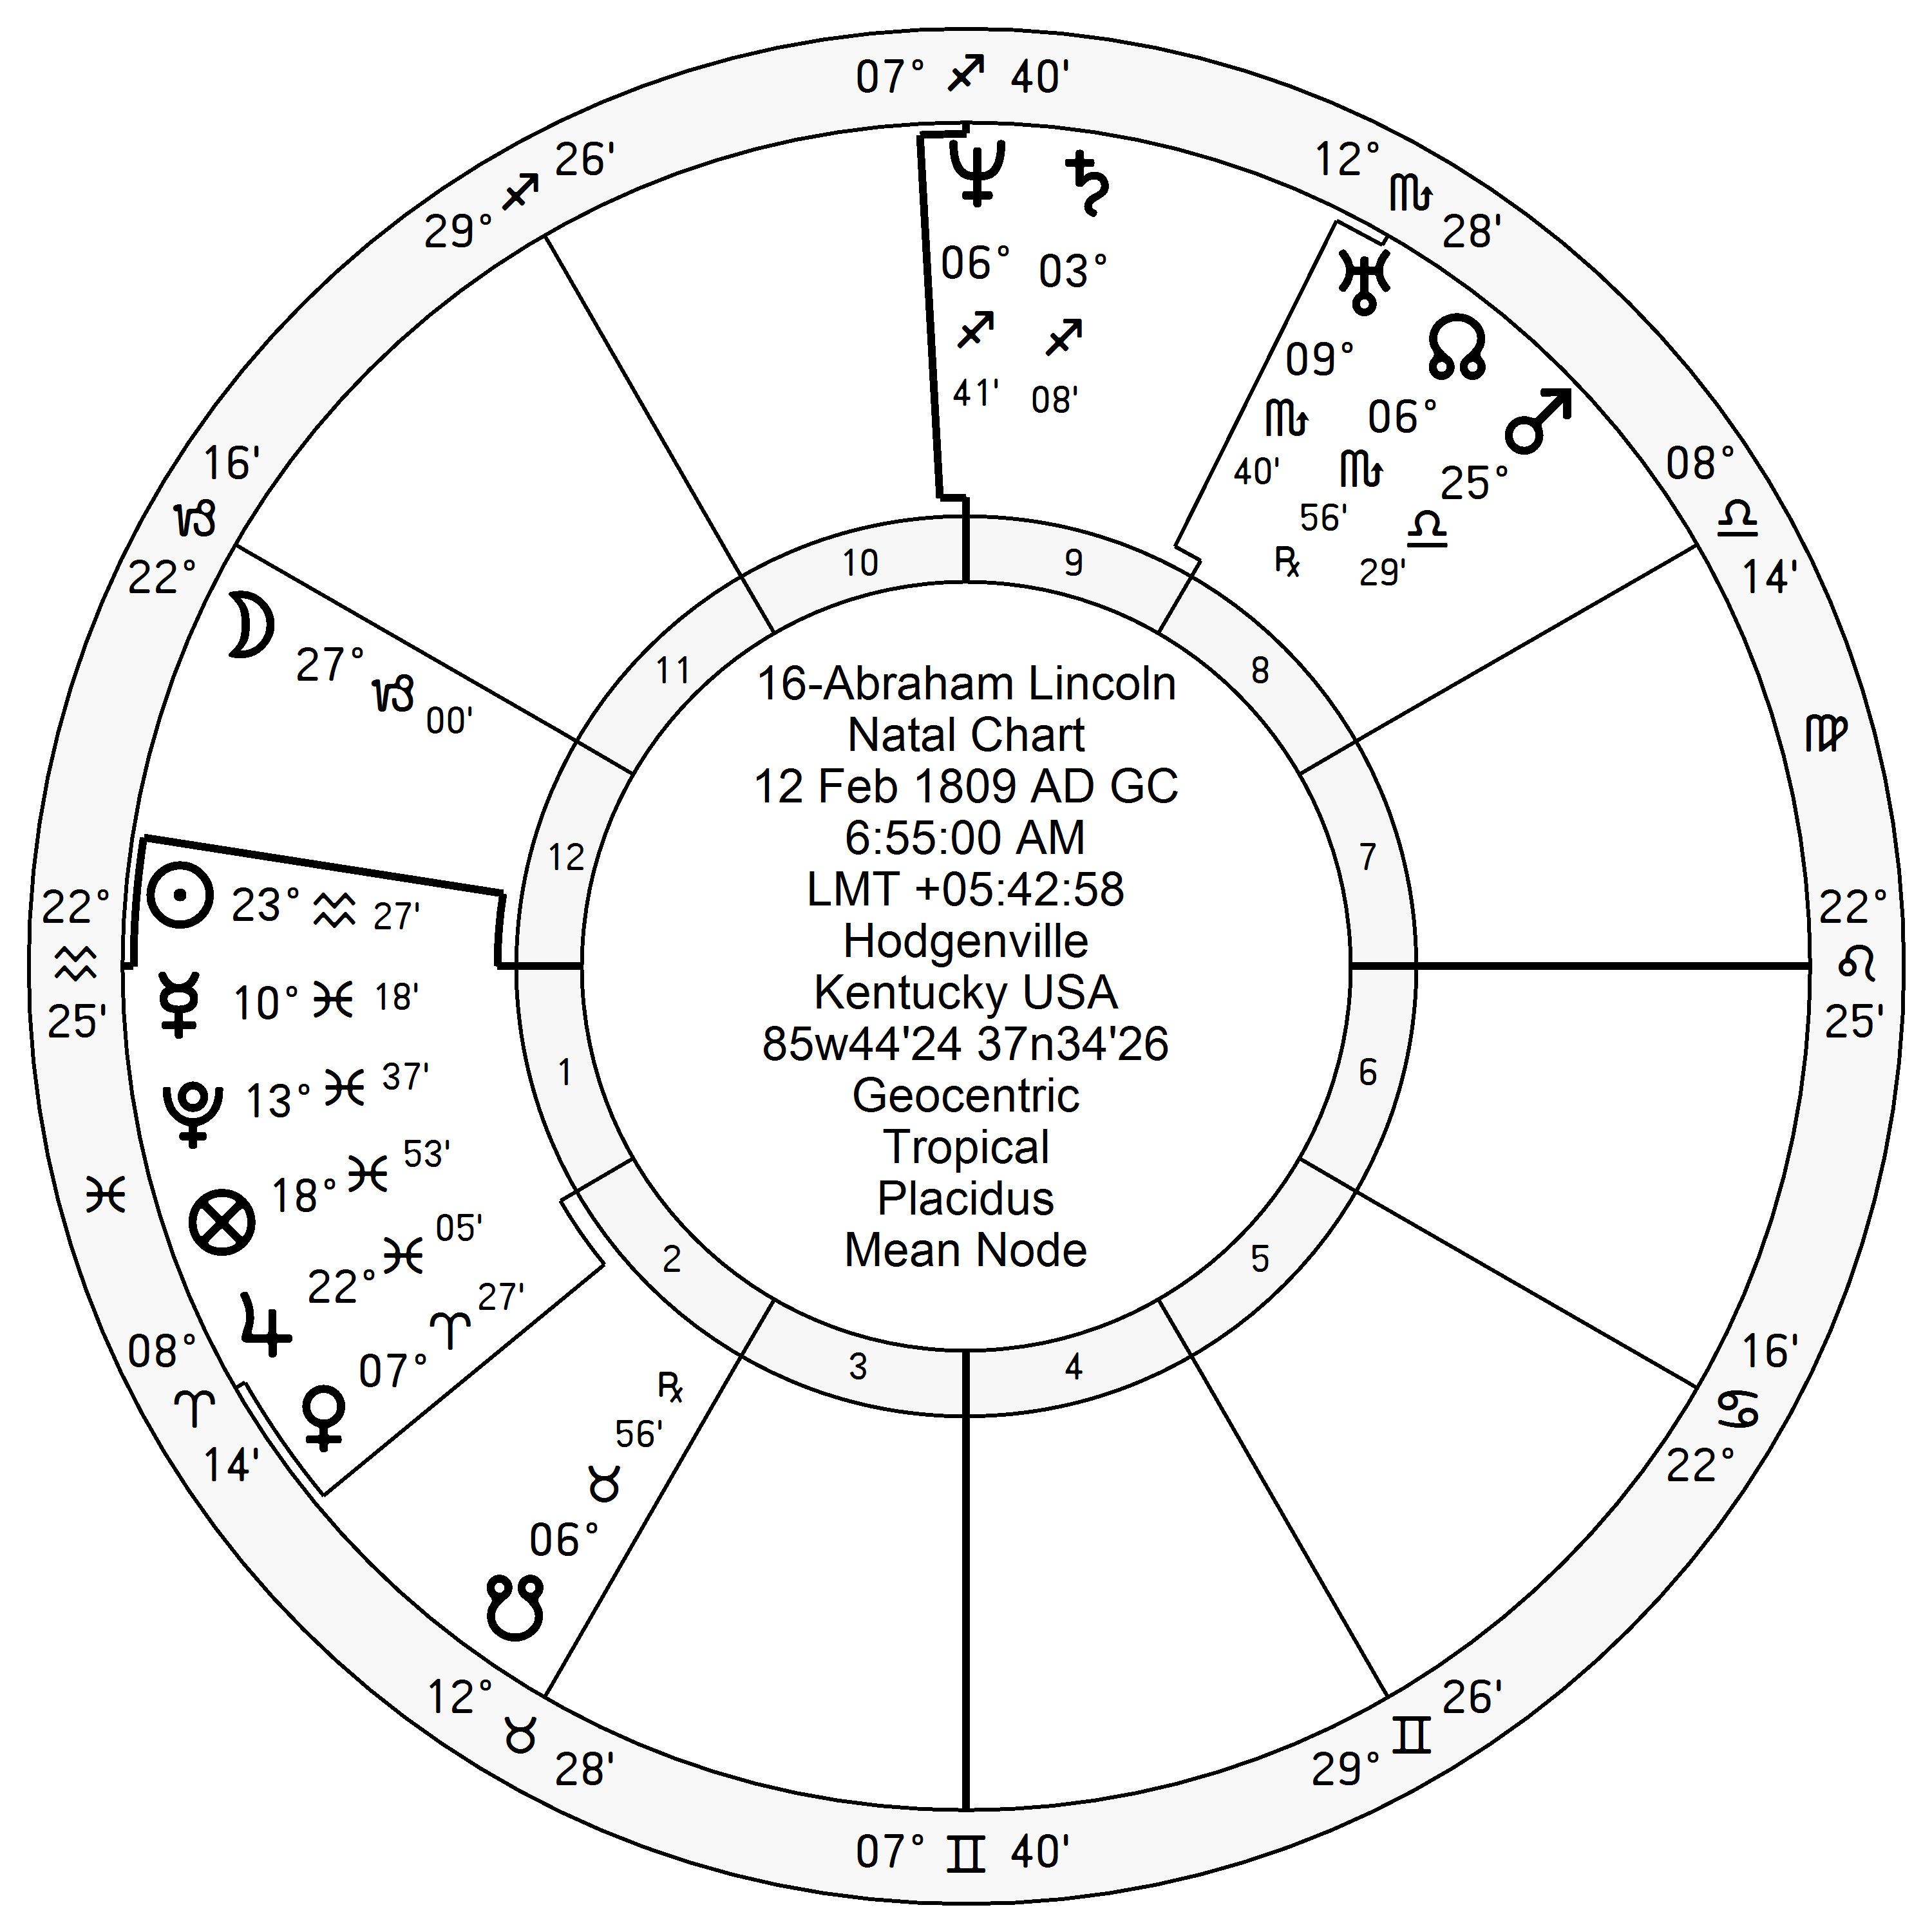
\includegraphics[width=0.9\textwidth]{charts/Lincoln.png}}
\fontsize{7pt}{8pt}\selectfont

\Mercury\, \Trine\, P10, \textbf{\Square\, N10} \\
\Venus\, \textbf{\Square\, P10}; in N1 partile \Trine\, MC

\column{0.48\textwidth}
\vspace{-1em}
{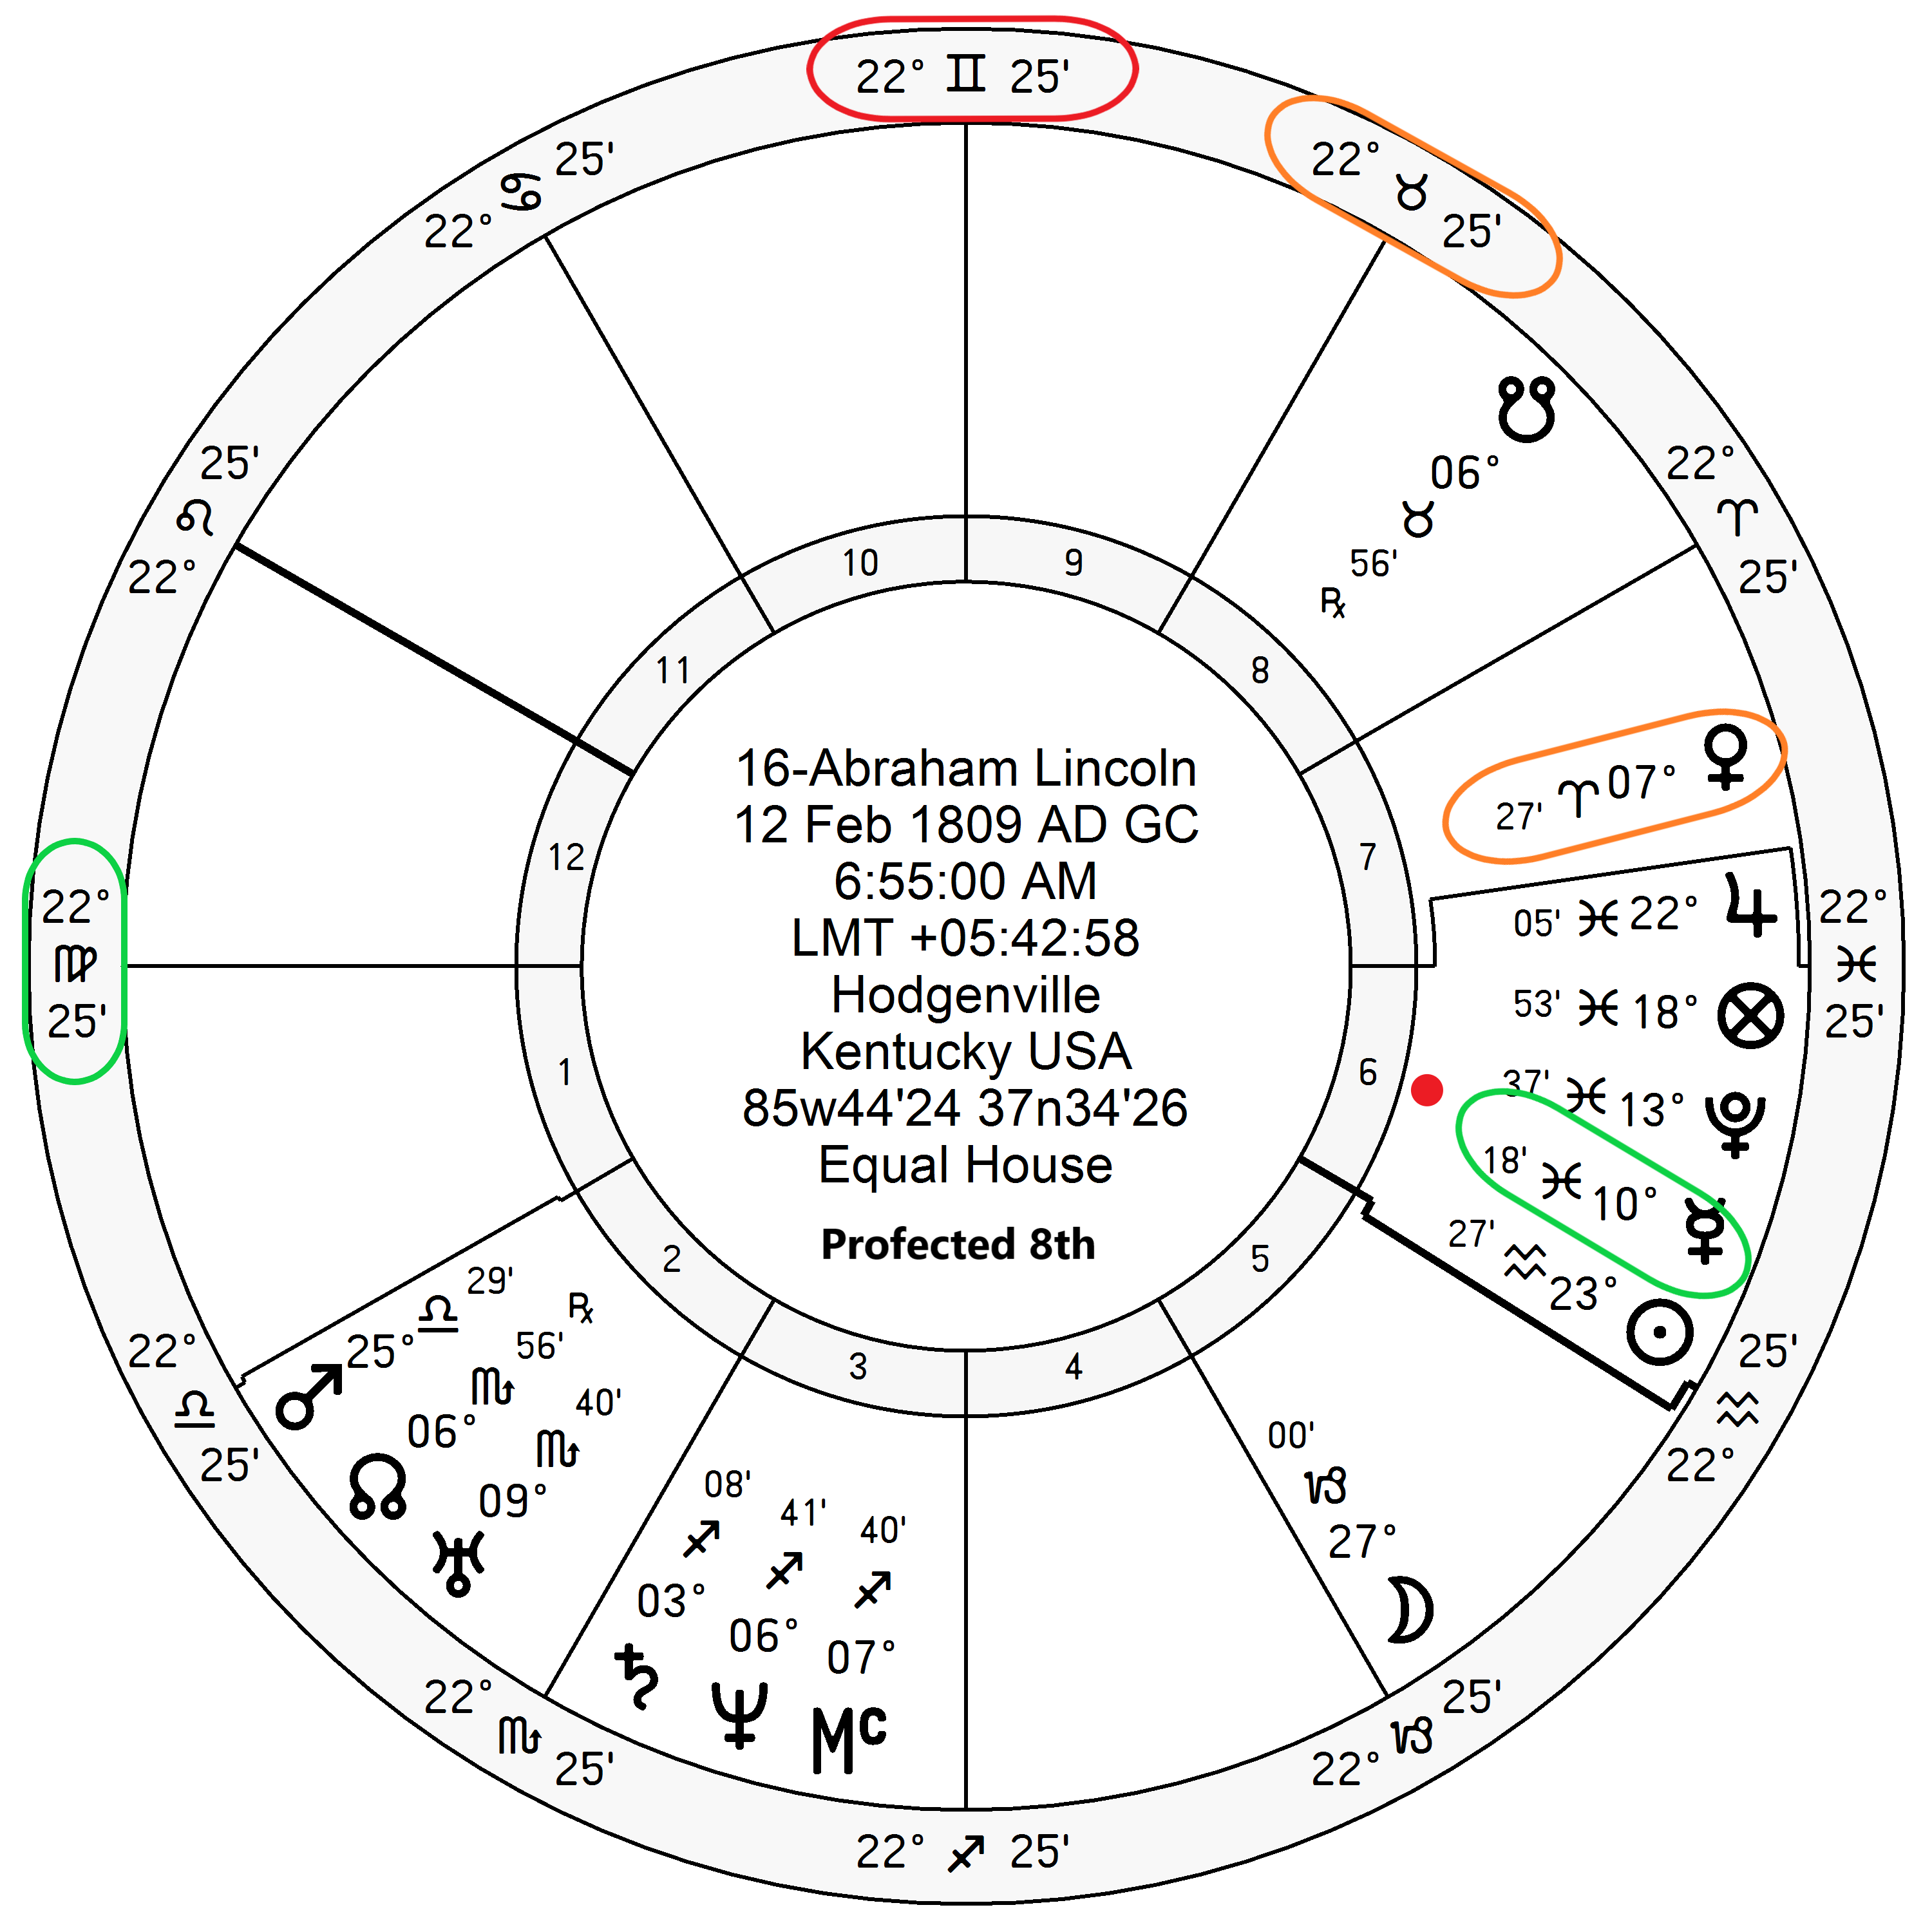
\includegraphics[width=0.9\textwidth]{charts/Lincoln-Prof-8th.png}}
\textbf{\dgreen P1=N7} $\Rightarrow$ \Mercury\, $\Rightarrow$ \textbf{\dgreen P6/N1} \\
\textbf{\red{P10}}=N4 $\Rightarrow$  \Mercury\, $\Rightarrow$  \textbf{\dgreen{P6/N1}} \\
PE=P9/N3 $\Rightarrow$  \Venus\, $\Rightarrow$  \textbf{\dgreen{P7/N1}}

\end{columns}
\end{frame}

% McClellan
\begin{frame}[t]{Election November 8, 1864: George McClellan}
\small
\begin{columns}[T, onlytextwidth]
\column{0.48\textwidth}
\vspace{-1em}
{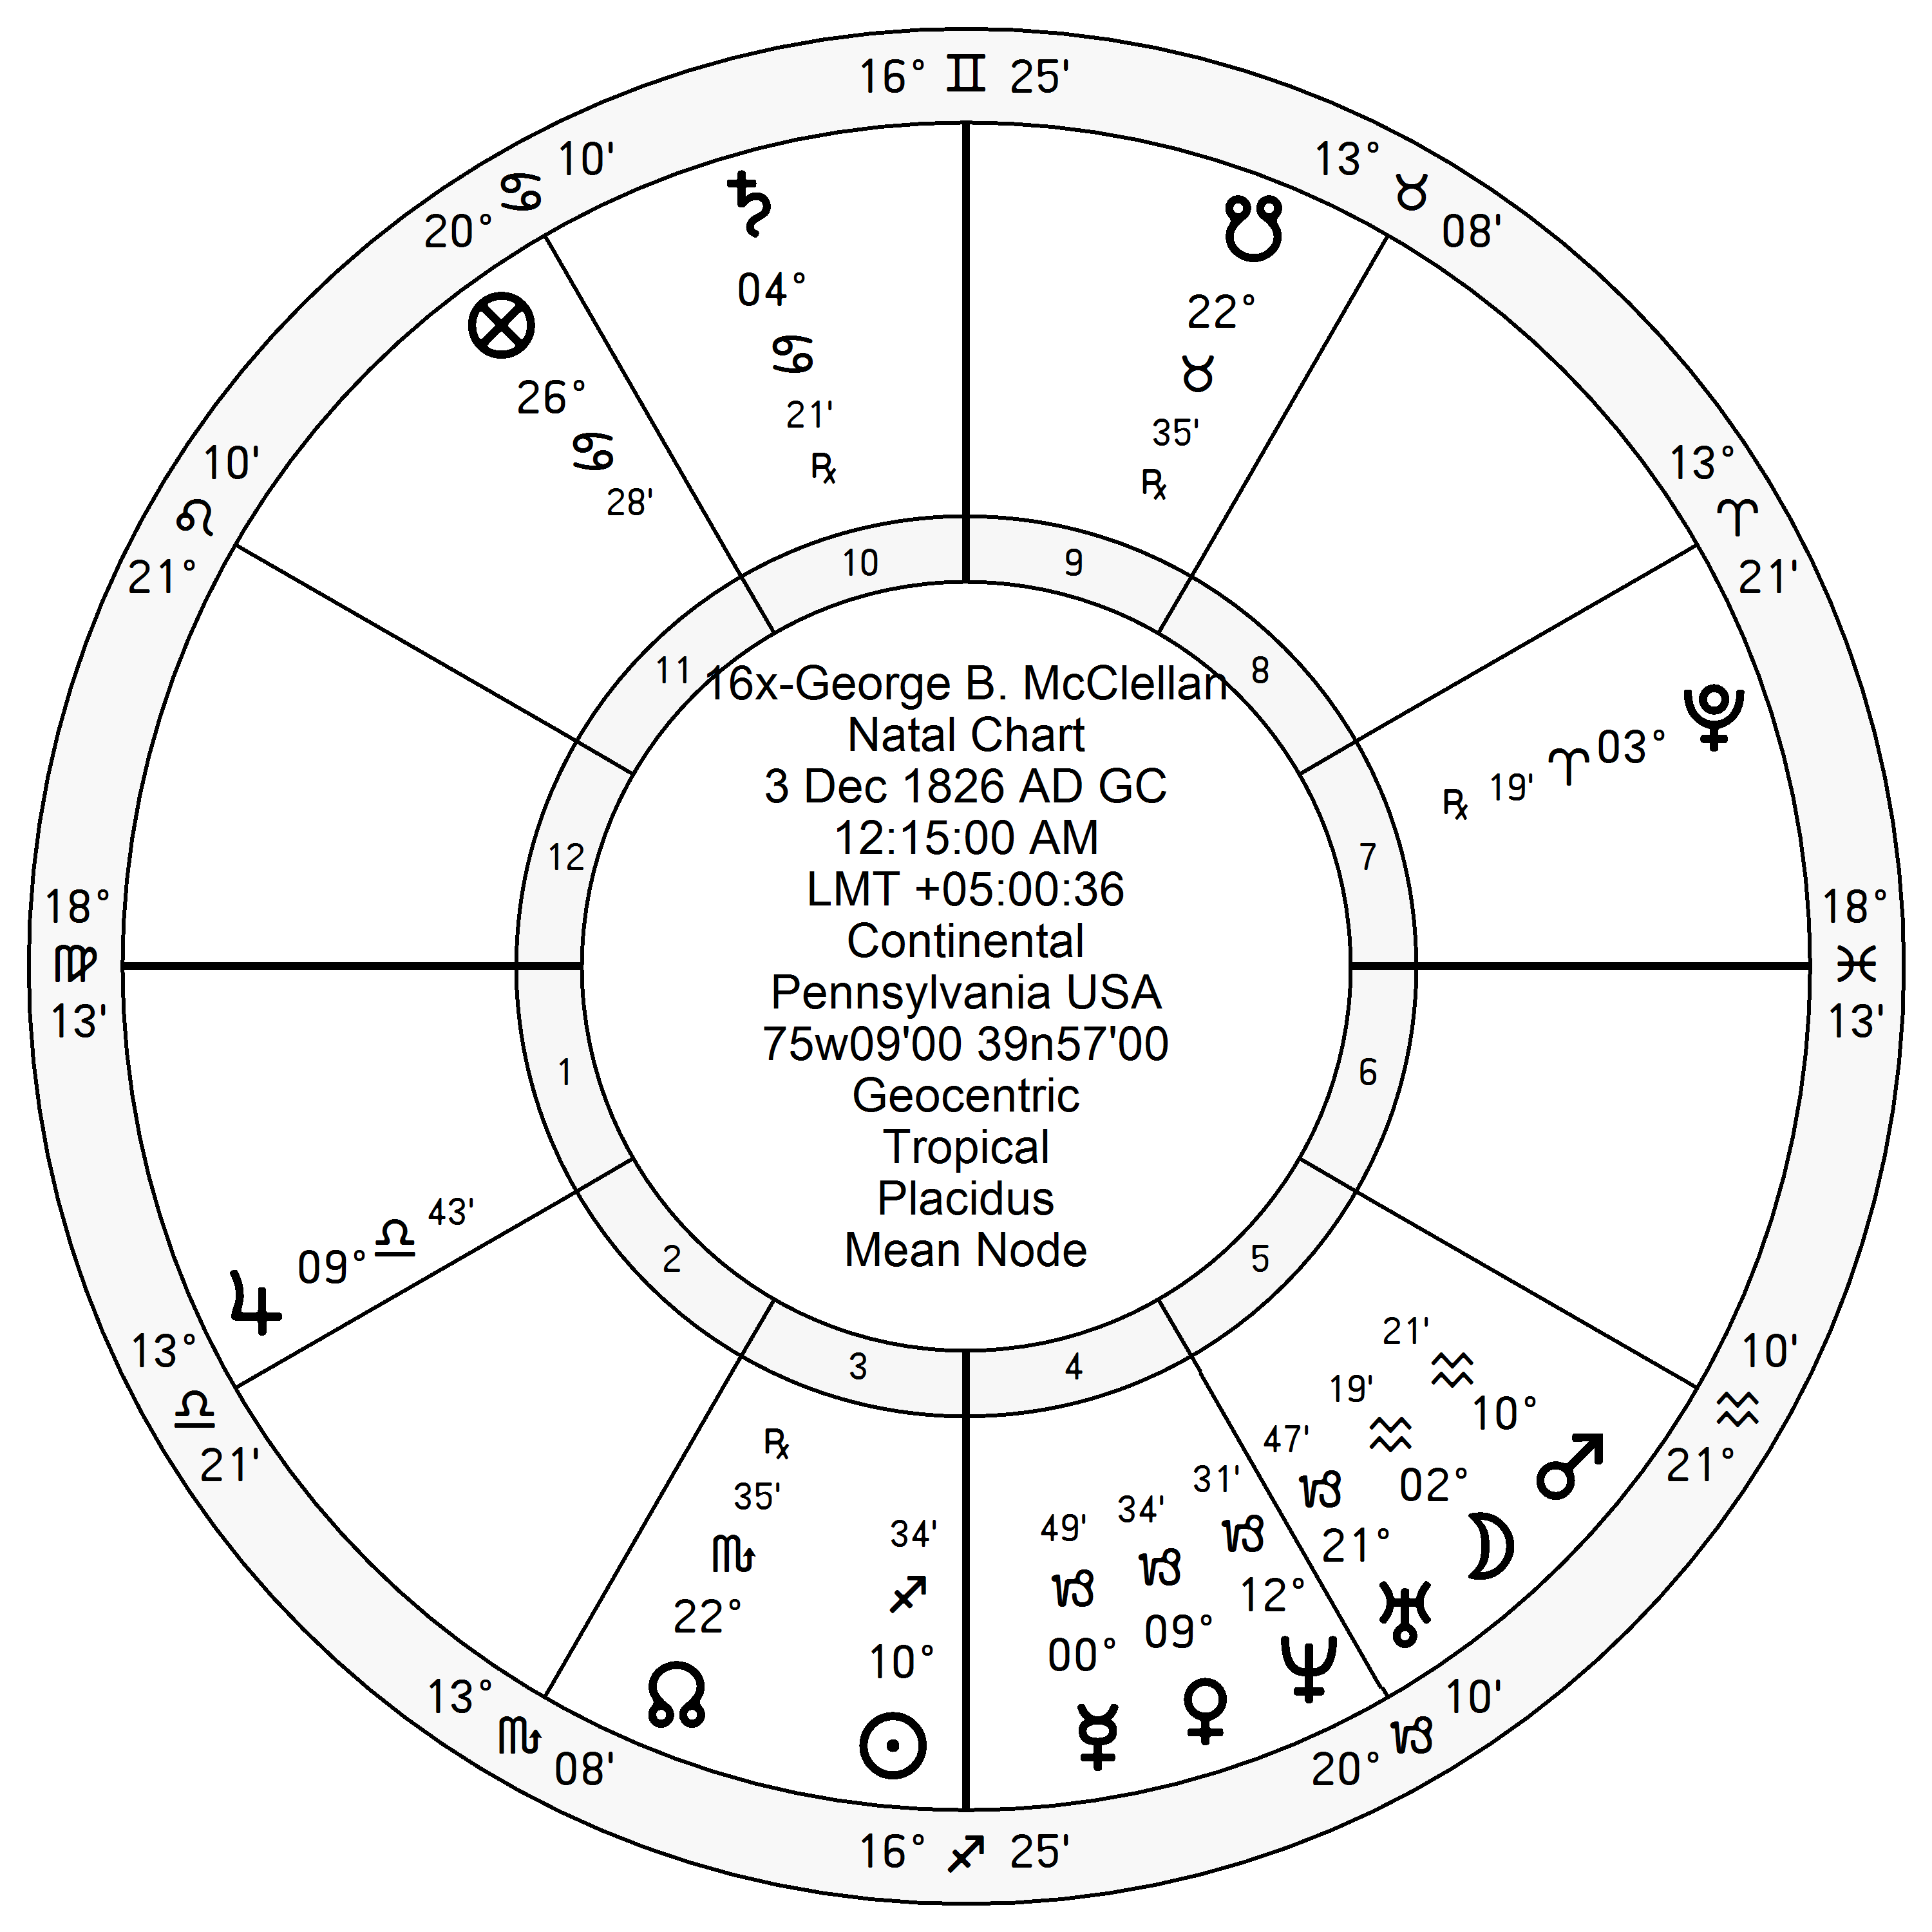
\includegraphics[width=0.9\textwidth]{charts/McClellan.png}}
\fontsize{8pt}{9pt}\selectfont

\Venus\, \Sextile\, P1, N1 \\
\Moon\, \textbf{\Opposition\, P10} \\
\Mercury\, \Sextile\, P1, N1 \\


\column{0.48\textwidth}
\vspace{-1em}
{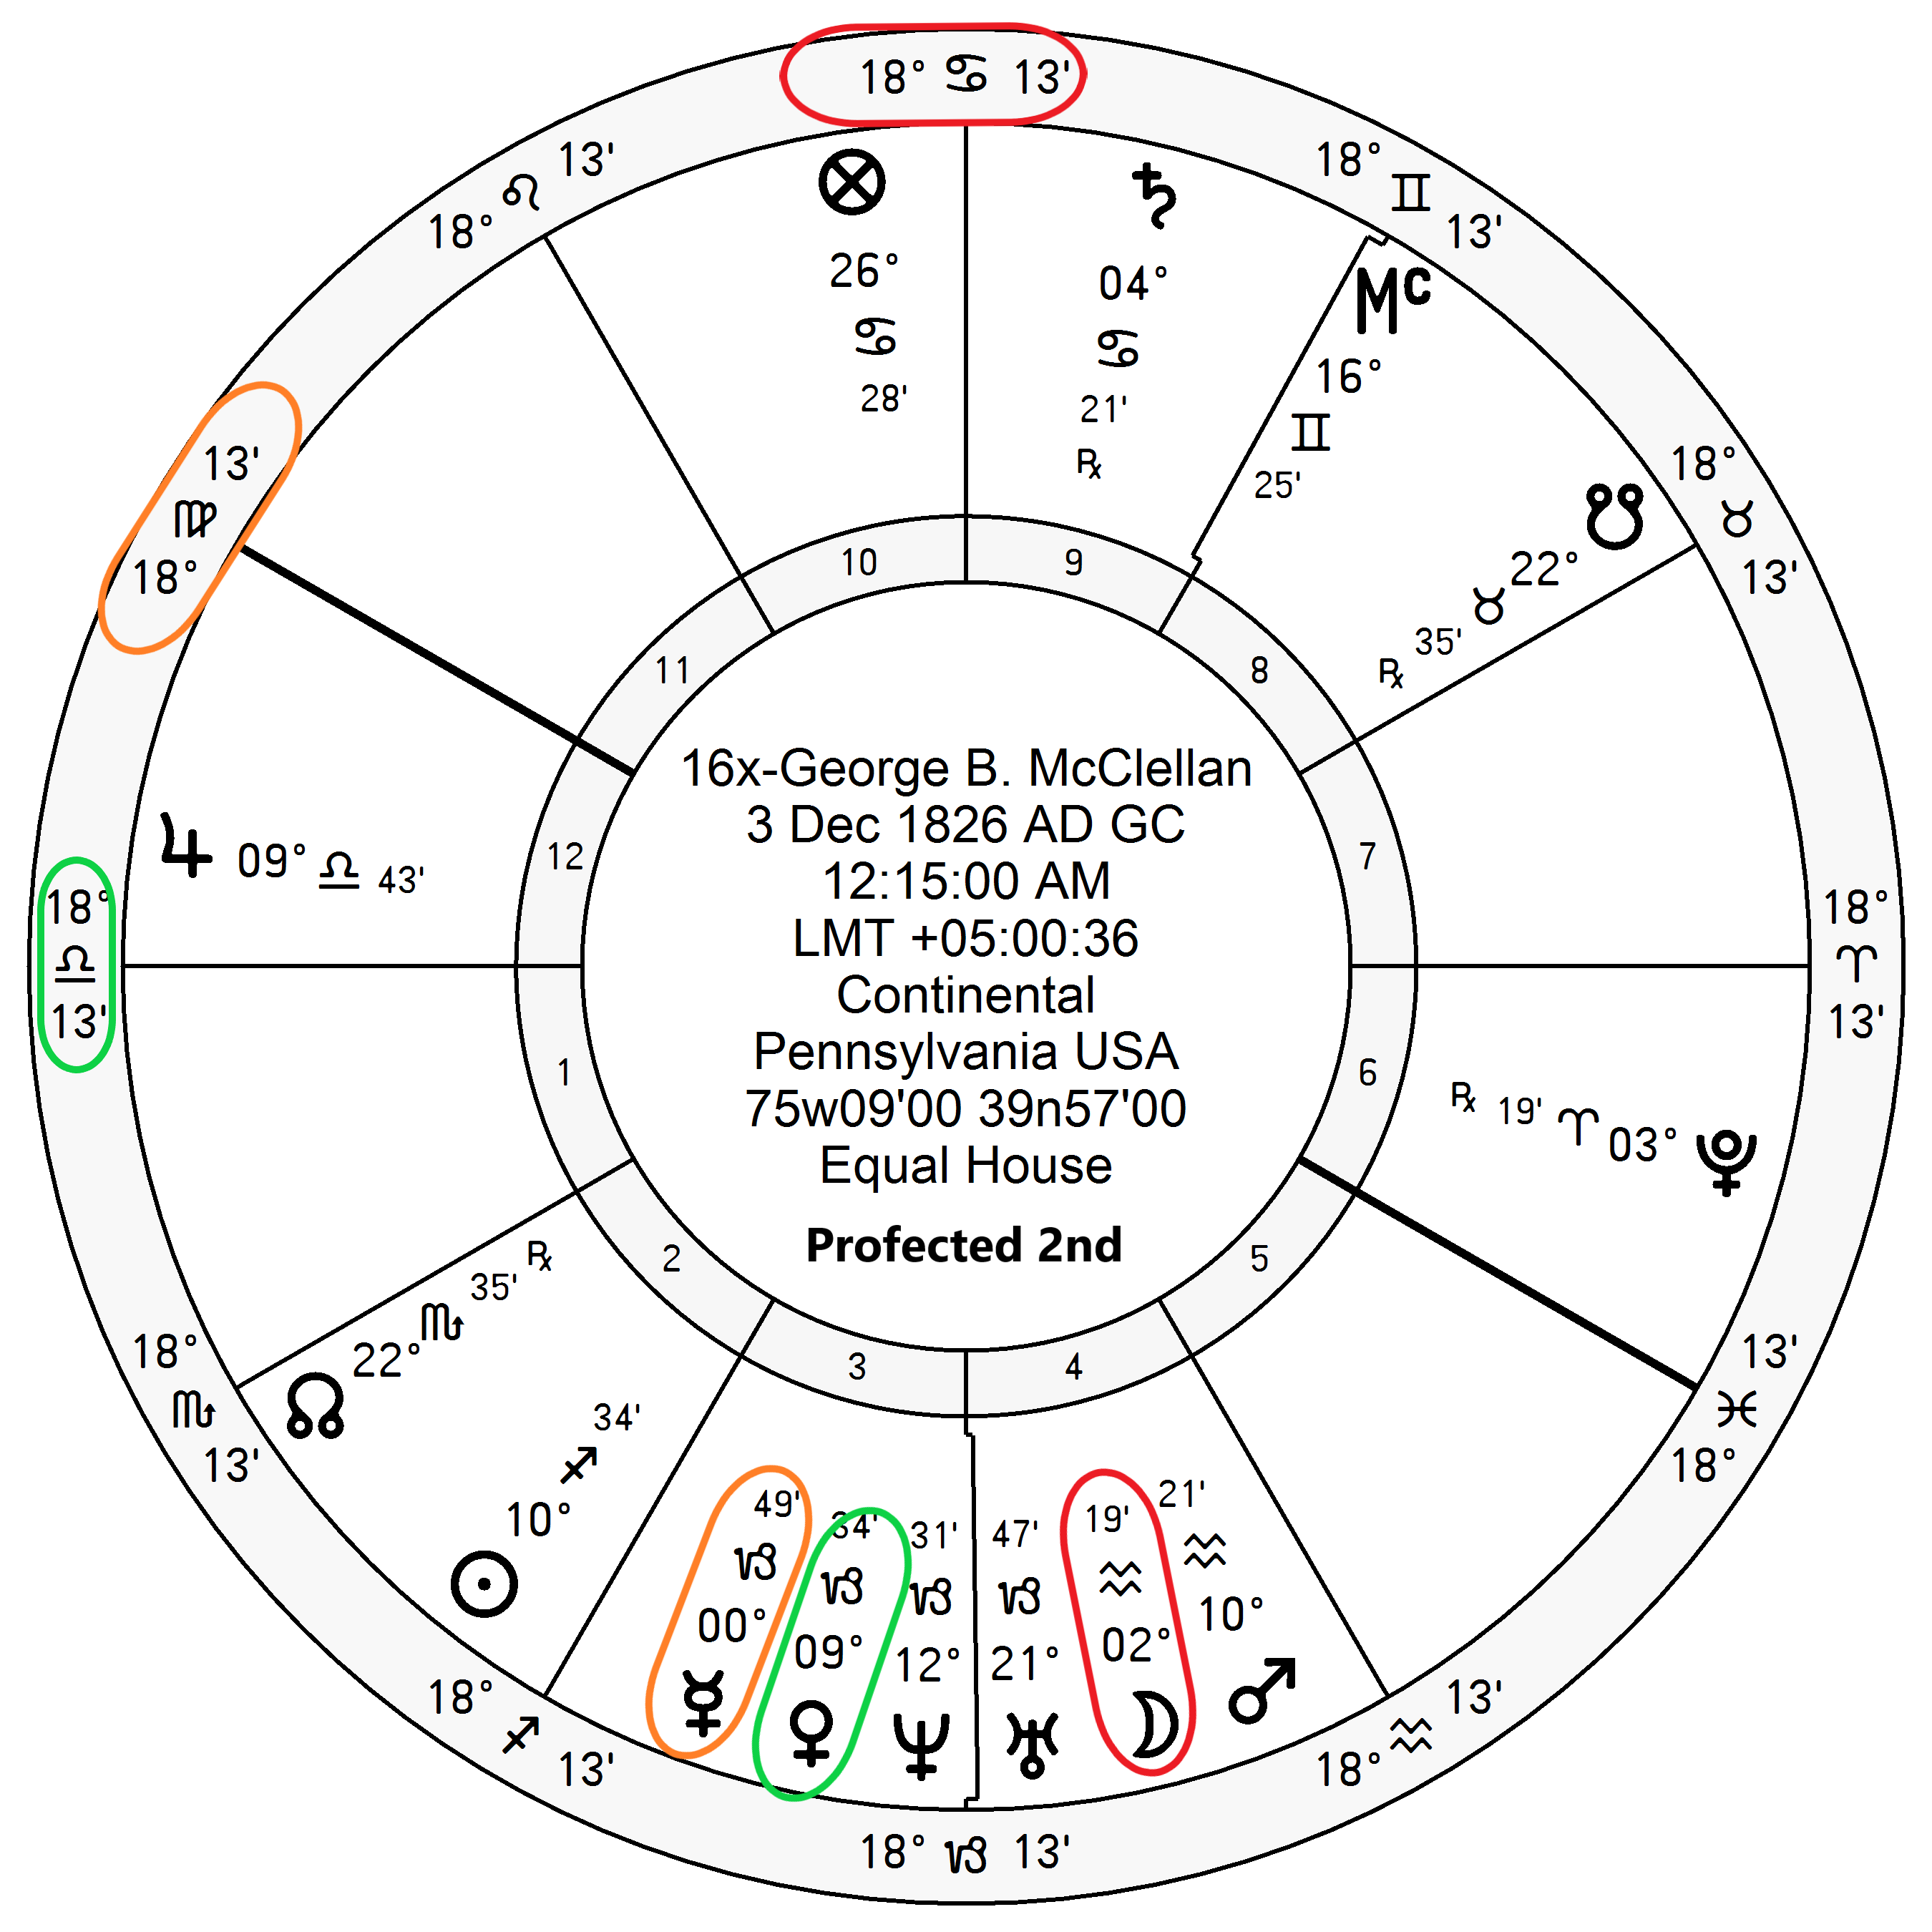
\includegraphics[width=0.9\textwidth]{charts/McClellan-Prof-2nd.png}}
\textbf{\dgreen P1}=N2 $\Rightarrow$ \Venus\, $\Rightarrow$ \textbf{\dgreen P3/N4}\\
\textbf{\red P10}=N11 $\Rightarrow$ \Moon\, $\Rightarrow$ \textbf{\dgreen P4}/N5\\
PE=P12/\textbf{\dgreen N1} $\Rightarrow$ \Mercury\, $\Rightarrow$ \textbf{\dgreen P3/N4}

\end{columns}
\end{frame}

%\subsection{Election November 3, 1896: *McKinley vs Bryan}
\begin{frame}[t]{Election November 3, 1896: *William McKinley}
\small
% Lincoln
\begin{columns}[T, onlytextwidth]
\column{0.48\textwidth}
\vspace{-1em}
{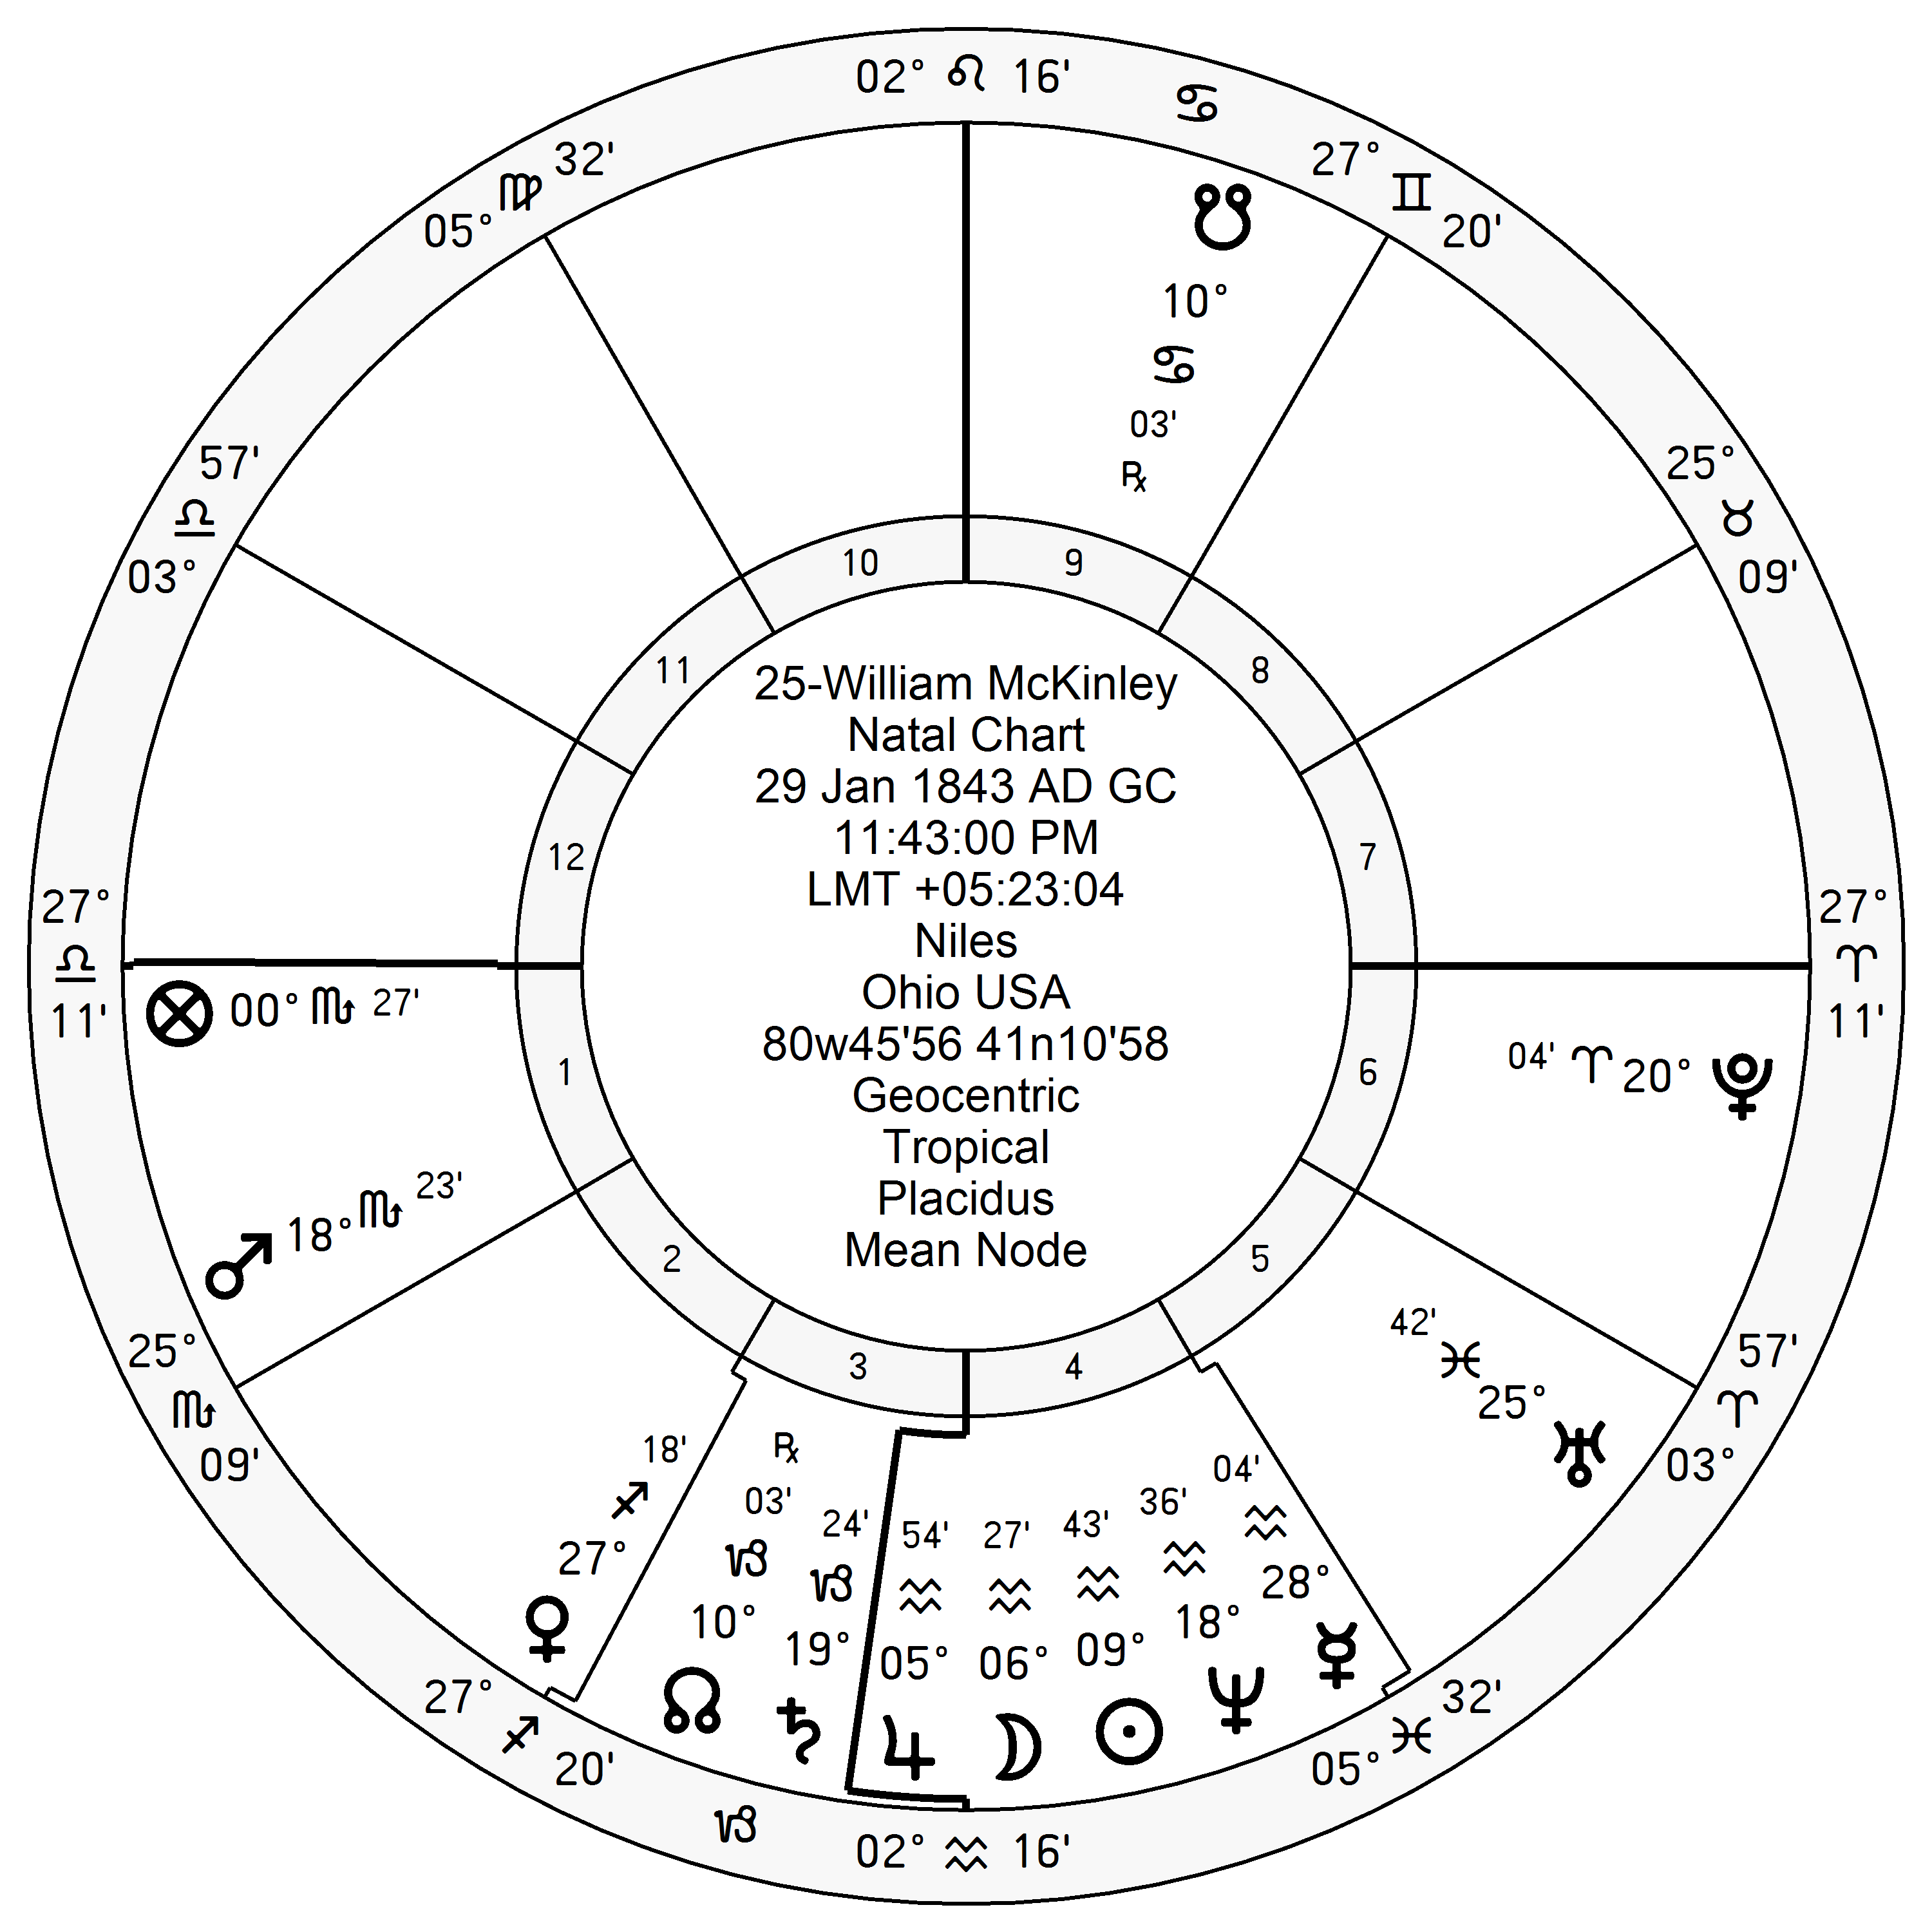
\includegraphics[width=0.9\textwidth]{charts/McKinley.png}}
\fontsize{8pt}{9pt}\selectfont

\Jupiter\, \Sextile\, P1, \Square\, N1, \Opposition\, N10. Disposited by \Saturn\, in domicile in P10.

\column{0.48\textwidth}
\vspace{-1em}
{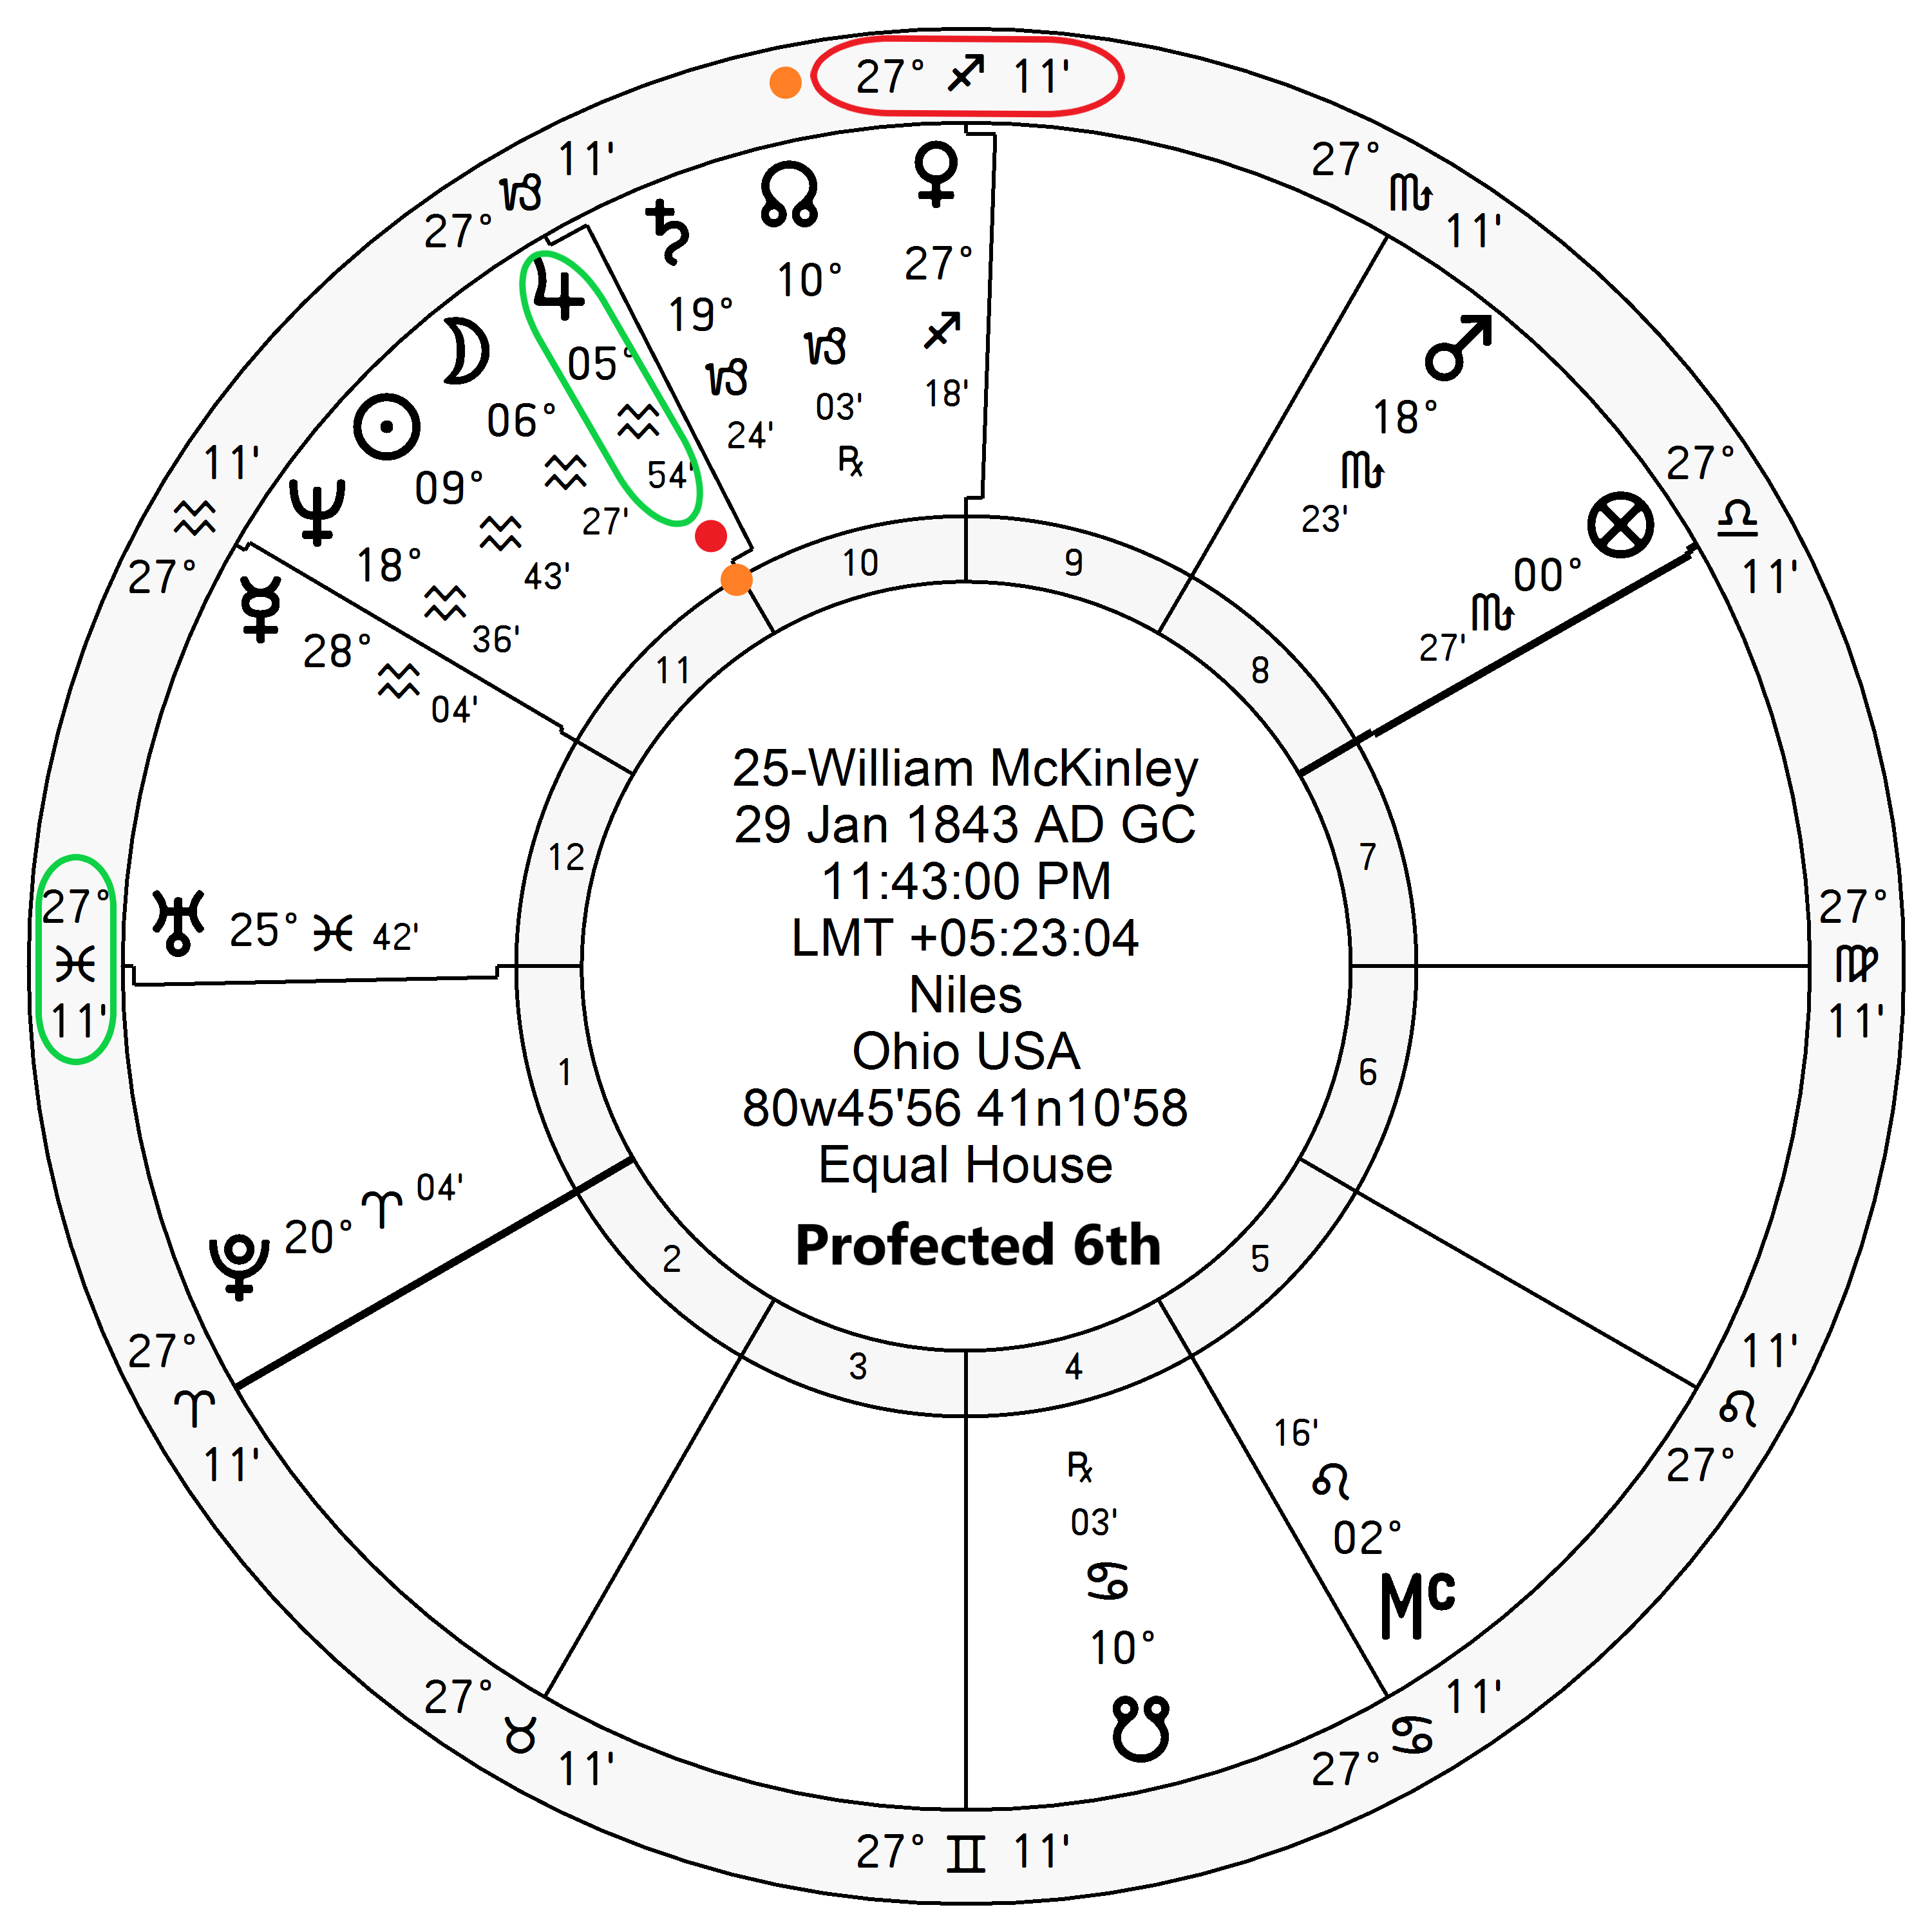
\includegraphics[width=0.9\textwidth]{charts/McKinley-Prof-6th.png}}
\textbf{\dgreen P1}=N5 
	$\Rightarrow$ \Jupiter\, $\Rightarrow$ \textbf{\dgreen P11/N4} \\
\textbf{\red P10=N3} 
	$\Rightarrow$  \Jupiter\, $\Rightarrow$  \textbf{\dgreen P11/N4} \\
PE=\textbf{\red P10/N3} 
	$\Rightarrow$  \Jupiter\, $\Rightarrow$  \textbf{\dgreen{P11/N4}}

\end{columns}
\end{frame}

% McClellan
\begin{frame}[t]{Election November 3, 1896: William Jennings Bryan}
\small
\begin{columns}[T, onlytextwidth]
\column{0.48\textwidth}
\vspace{-1em}
{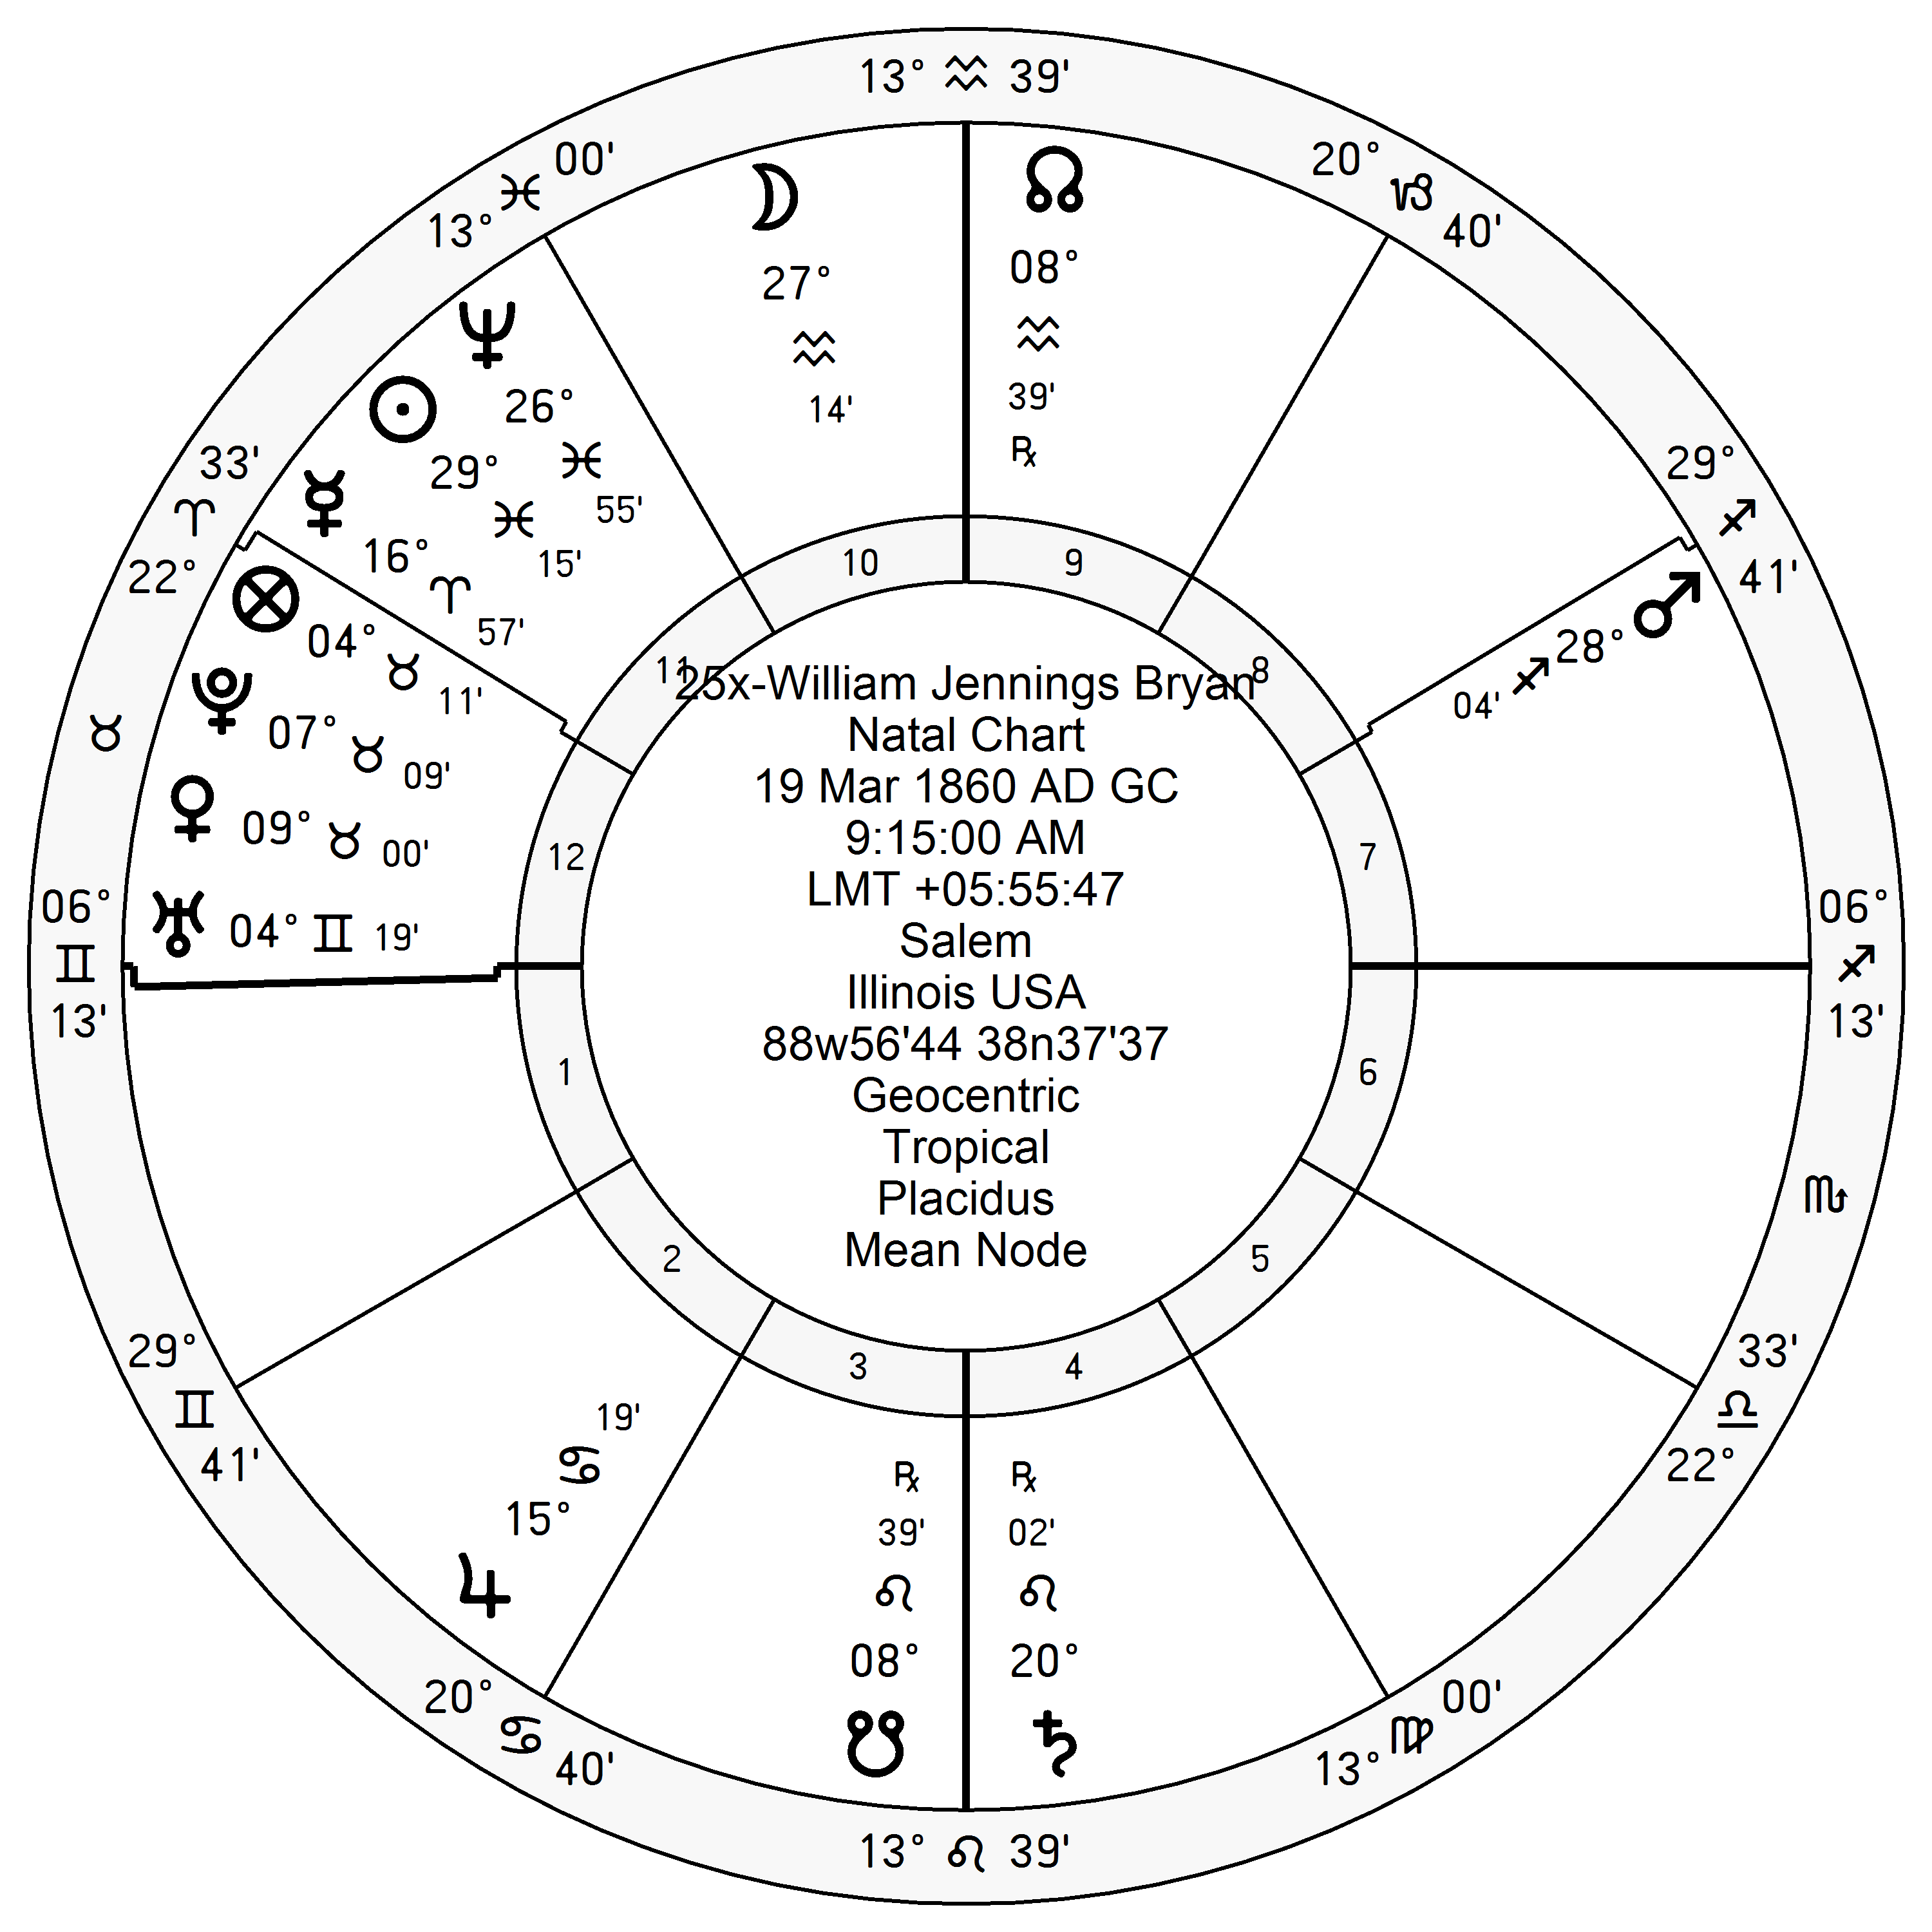
\includegraphics[width=0.9\textwidth]{charts/Bryan.png}}
\fontsize{8pt}{9pt}\selectfont

\Mercury\, is \Sextile\, N10; \Sextile\, P1. \\
\Jupiter\, \Trine\, P10, N10. \\
\Saturn\, averse to P10, \Opposition\, N10; \Sextile\, P1, N1. \\
In the profection, \Saturn\, and the \SouthNode\, are in the same sign and house; the South Node tends to be destructive.

\column{0.48\textwidth}
\vspace{-1em}
{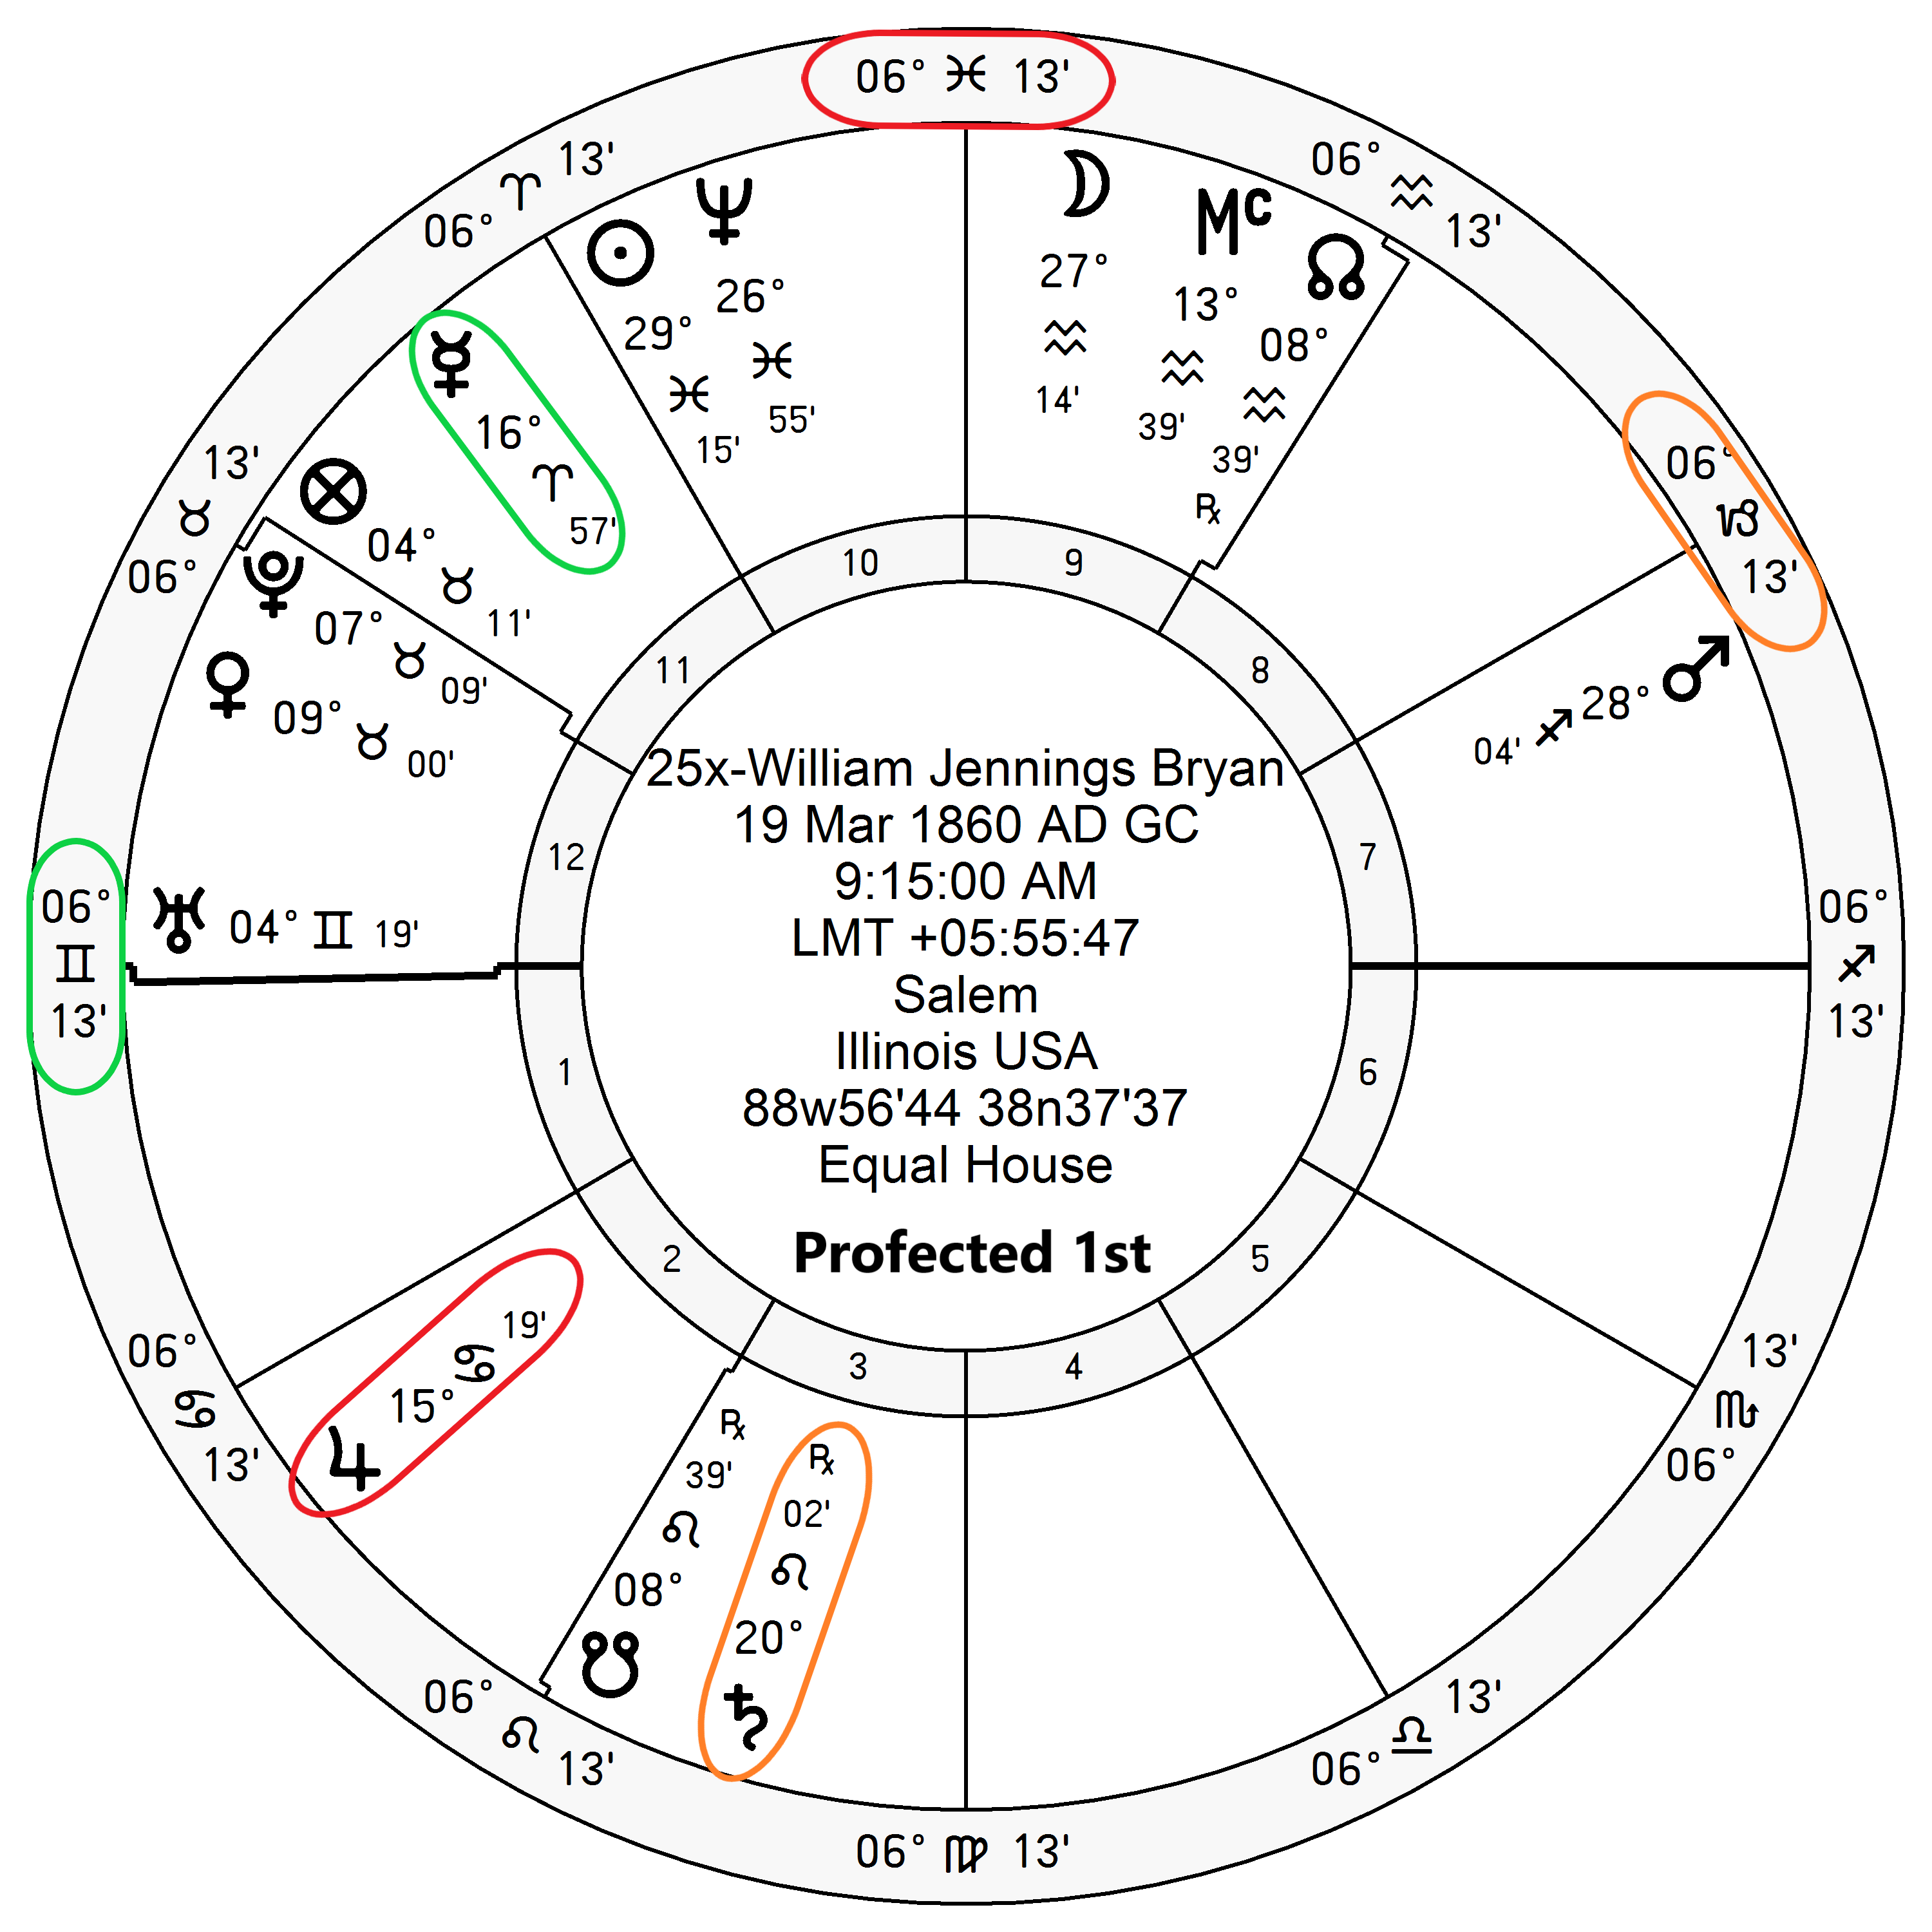
\includegraphics[width=0.9\textwidth]{charts/Bryan-Prof-1st.png}}
\textbf{\dgreen P1=N1} 
	$\Rightarrow$ \Mercury\, $\Rightarrow$ P11/N11\\
\textbf{\red P10=N10}
	$\Rightarrow$ \Jupiter\, $\Rightarrow$ P2/N2\\
PE=P8/N8 
	$\Rightarrow$ \Saturn\,\Retrograde $\Rightarrow$ P3/N4
\end{columns}
\end{frame}

%\subsection{Election November 6, 1900: *McKinley vs Bryan}
\begin{frame}[t]{Election November 6, 1900: *William McKinley}
\small
% McKinley
\begin{columns}[T, onlytextwidth]
\column{0.48\textwidth}
\vspace{-1em}
{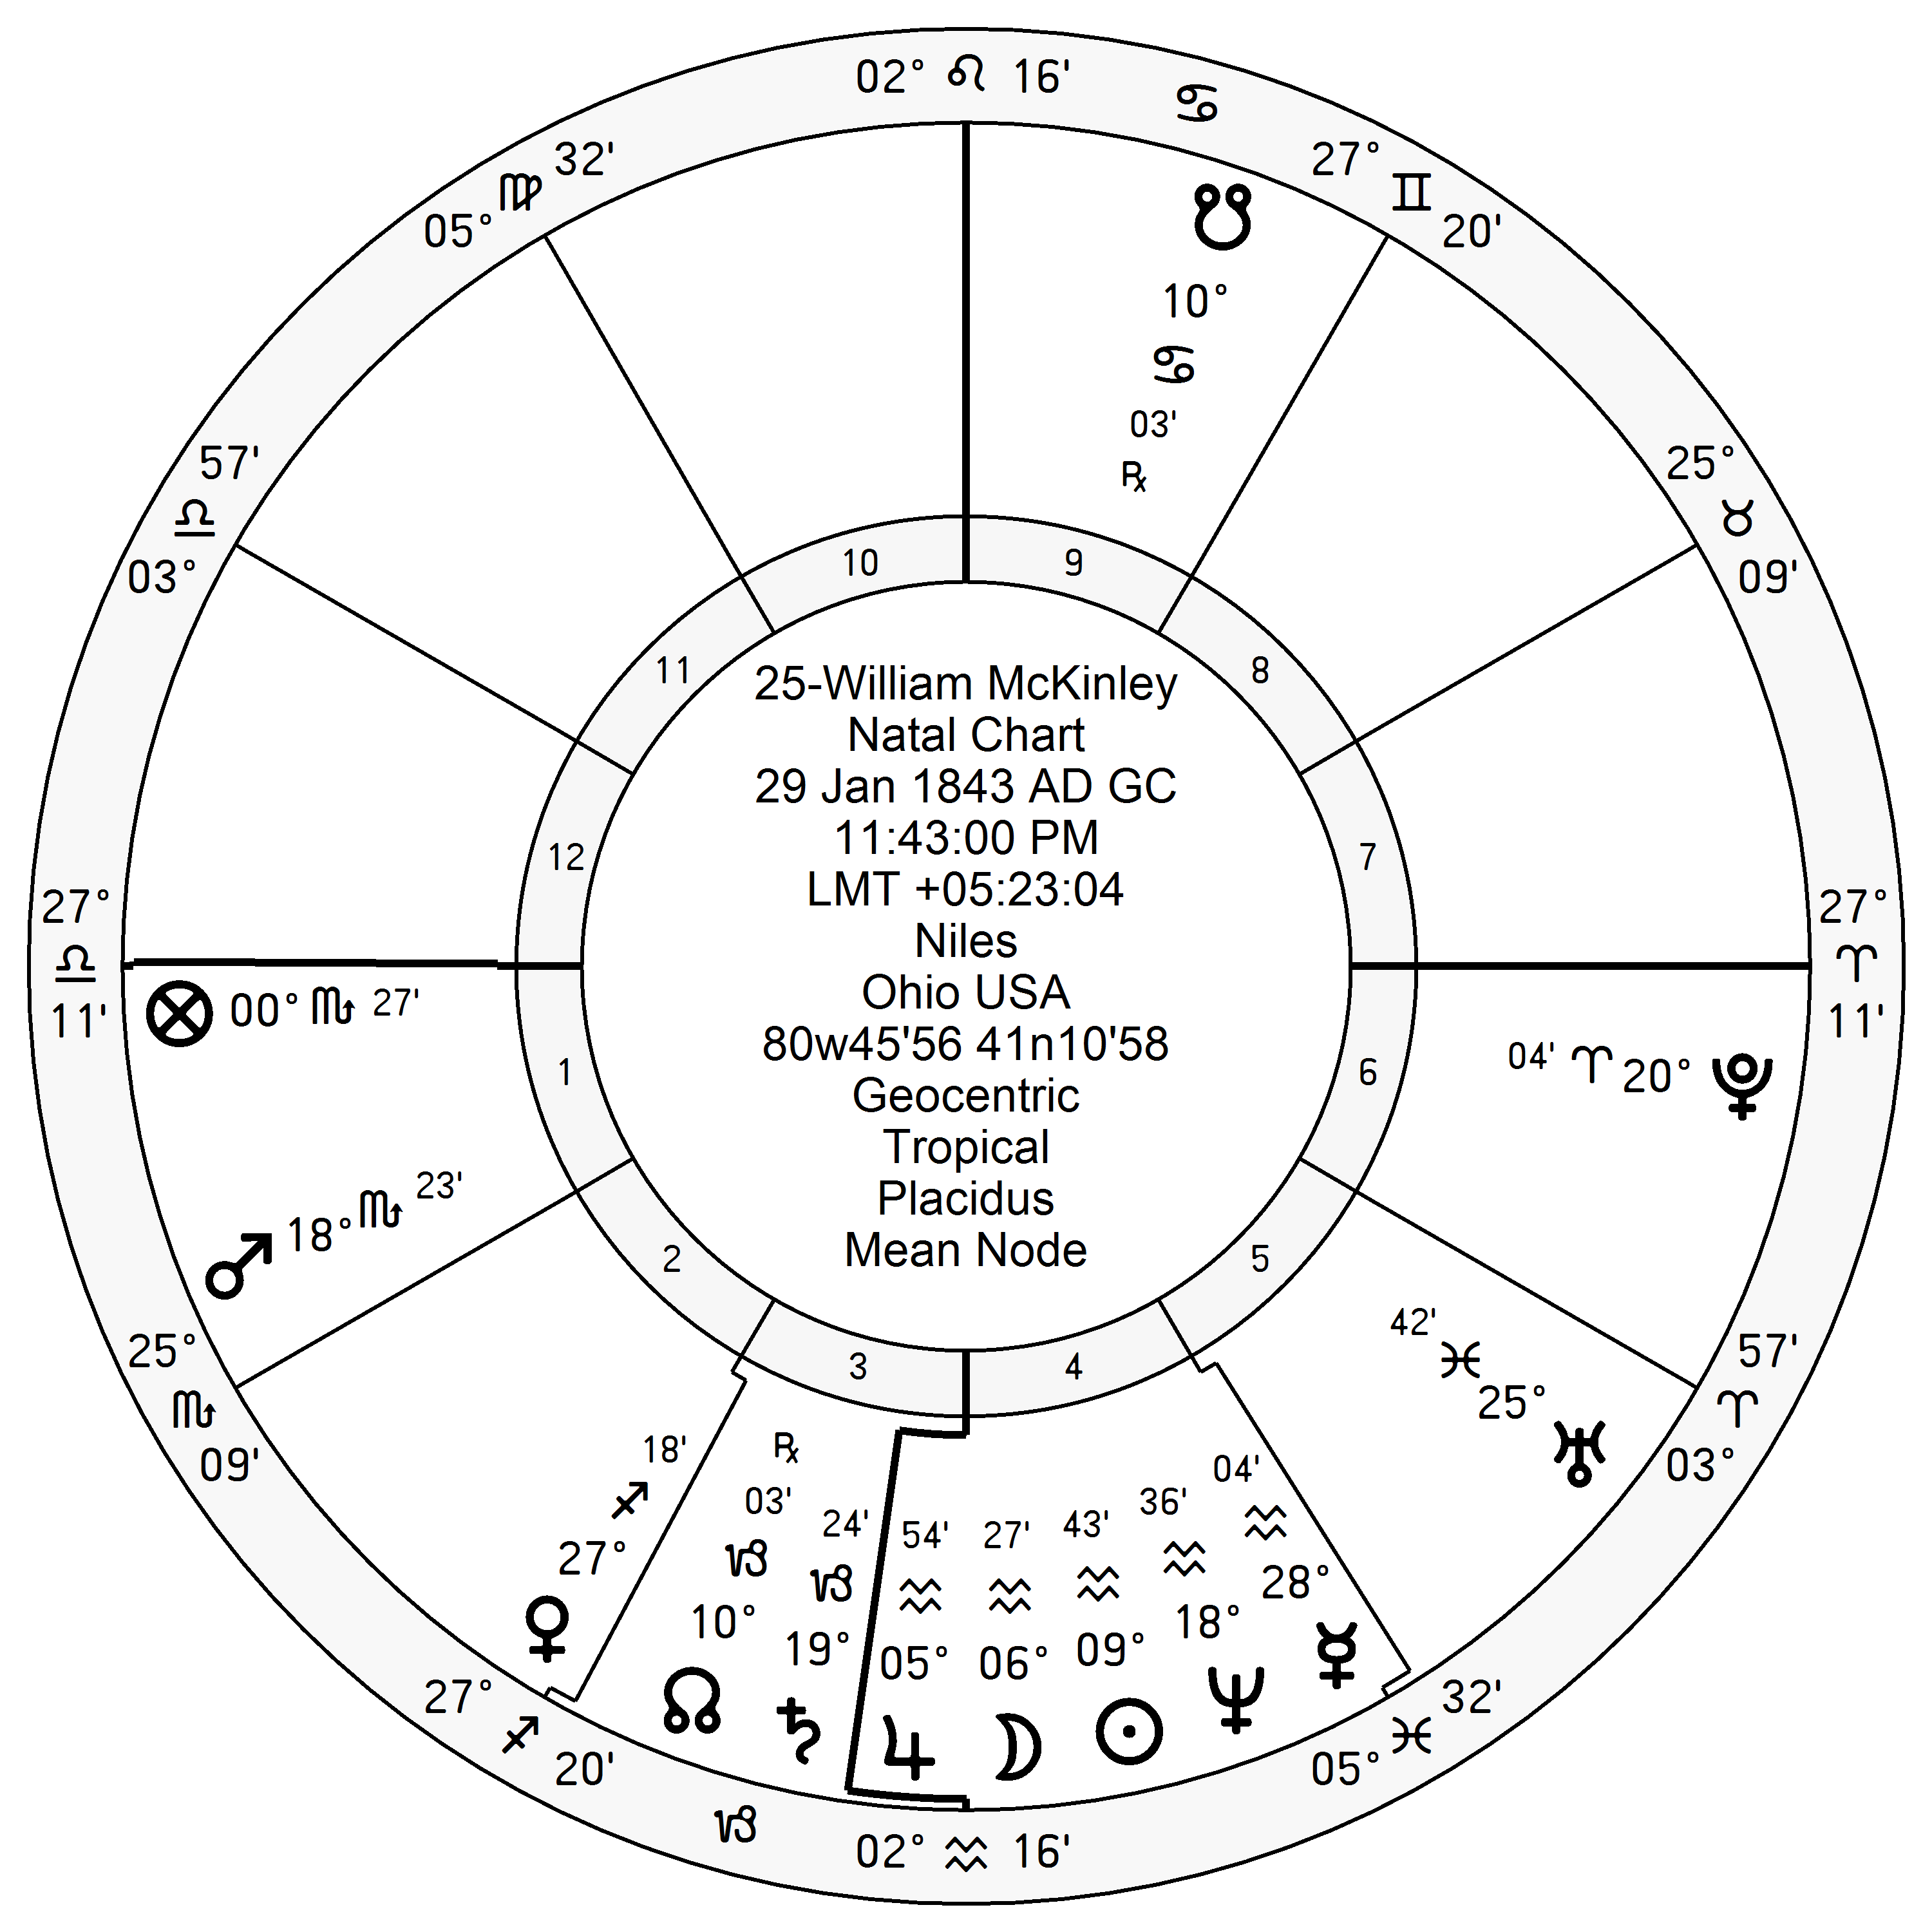
\includegraphics[width=0.9\textwidth]{charts/McKinley.png}}
\fontsize{7pt}{8pt}\selectfont

\Moon\, \Opposition\, P1, N10. The \Moon's combustion does not appear to create a problem; possibly protected by the \Jupiter\, \Conjunction. \\
\Mars\, \Opposition\, P10, \Square\, N10; \Square\, P1, in N1.

\column{0.48\textwidth}
\vspace{-1em}
{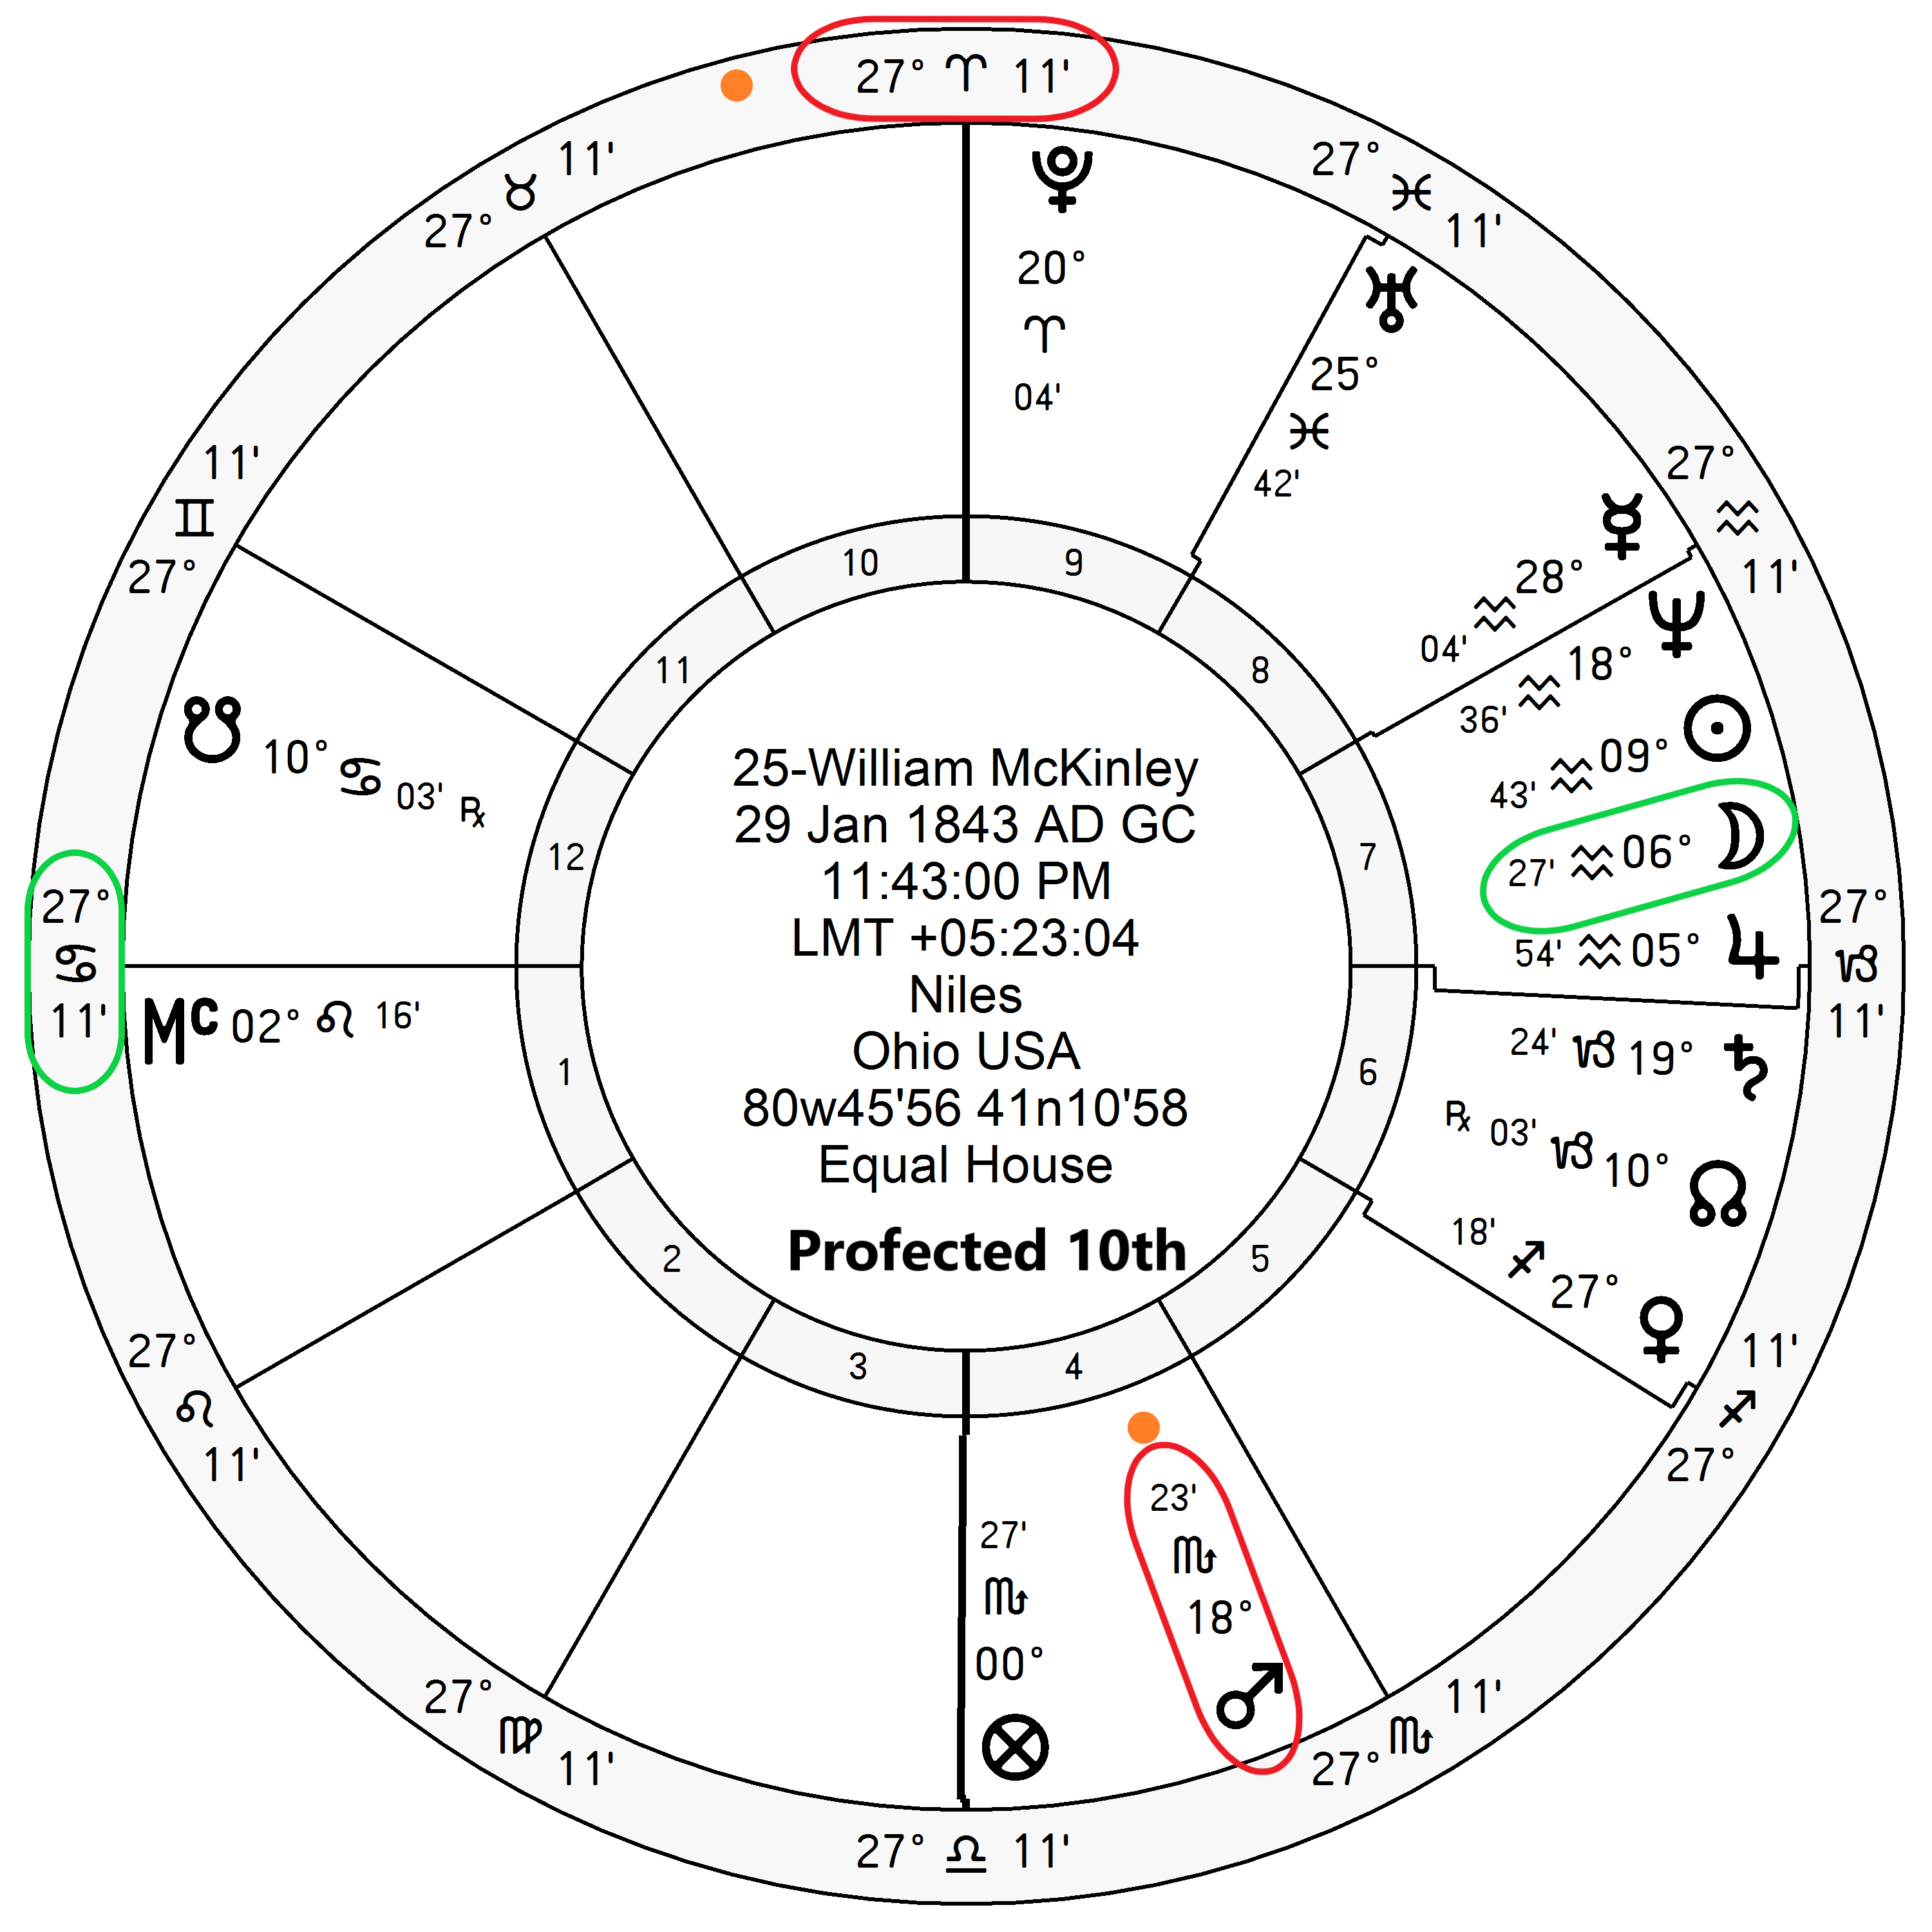
\includegraphics[width=0.9\textwidth]{charts/McKinley-Prof-10th.png}}
\textbf{\dgreen P1}=N9 
	$\Rightarrow$ \Moon\, $\Rightarrow$ \textbf{\red P7}/\textbf{\dgreen N4} \\
\textbf{\red P10=N7} 
	$\Rightarrow$  \Mars\, $\Rightarrow$  \textbf{\dgreen P4/N1} \\
PE=\textbf{\red P10/N7} 
	$\Rightarrow$  \Mars\, $\Rightarrow$  \textbf{\dgreen{P4/N1}}
\end{columns}
\end{frame}

% Bryan
\begin{frame}[t]{Election November 6, 1900: William Jennings Bryan}
\small
\begin{columns}[T, onlytextwidth]
\column{0.48\textwidth}
\vspace{-1em}
{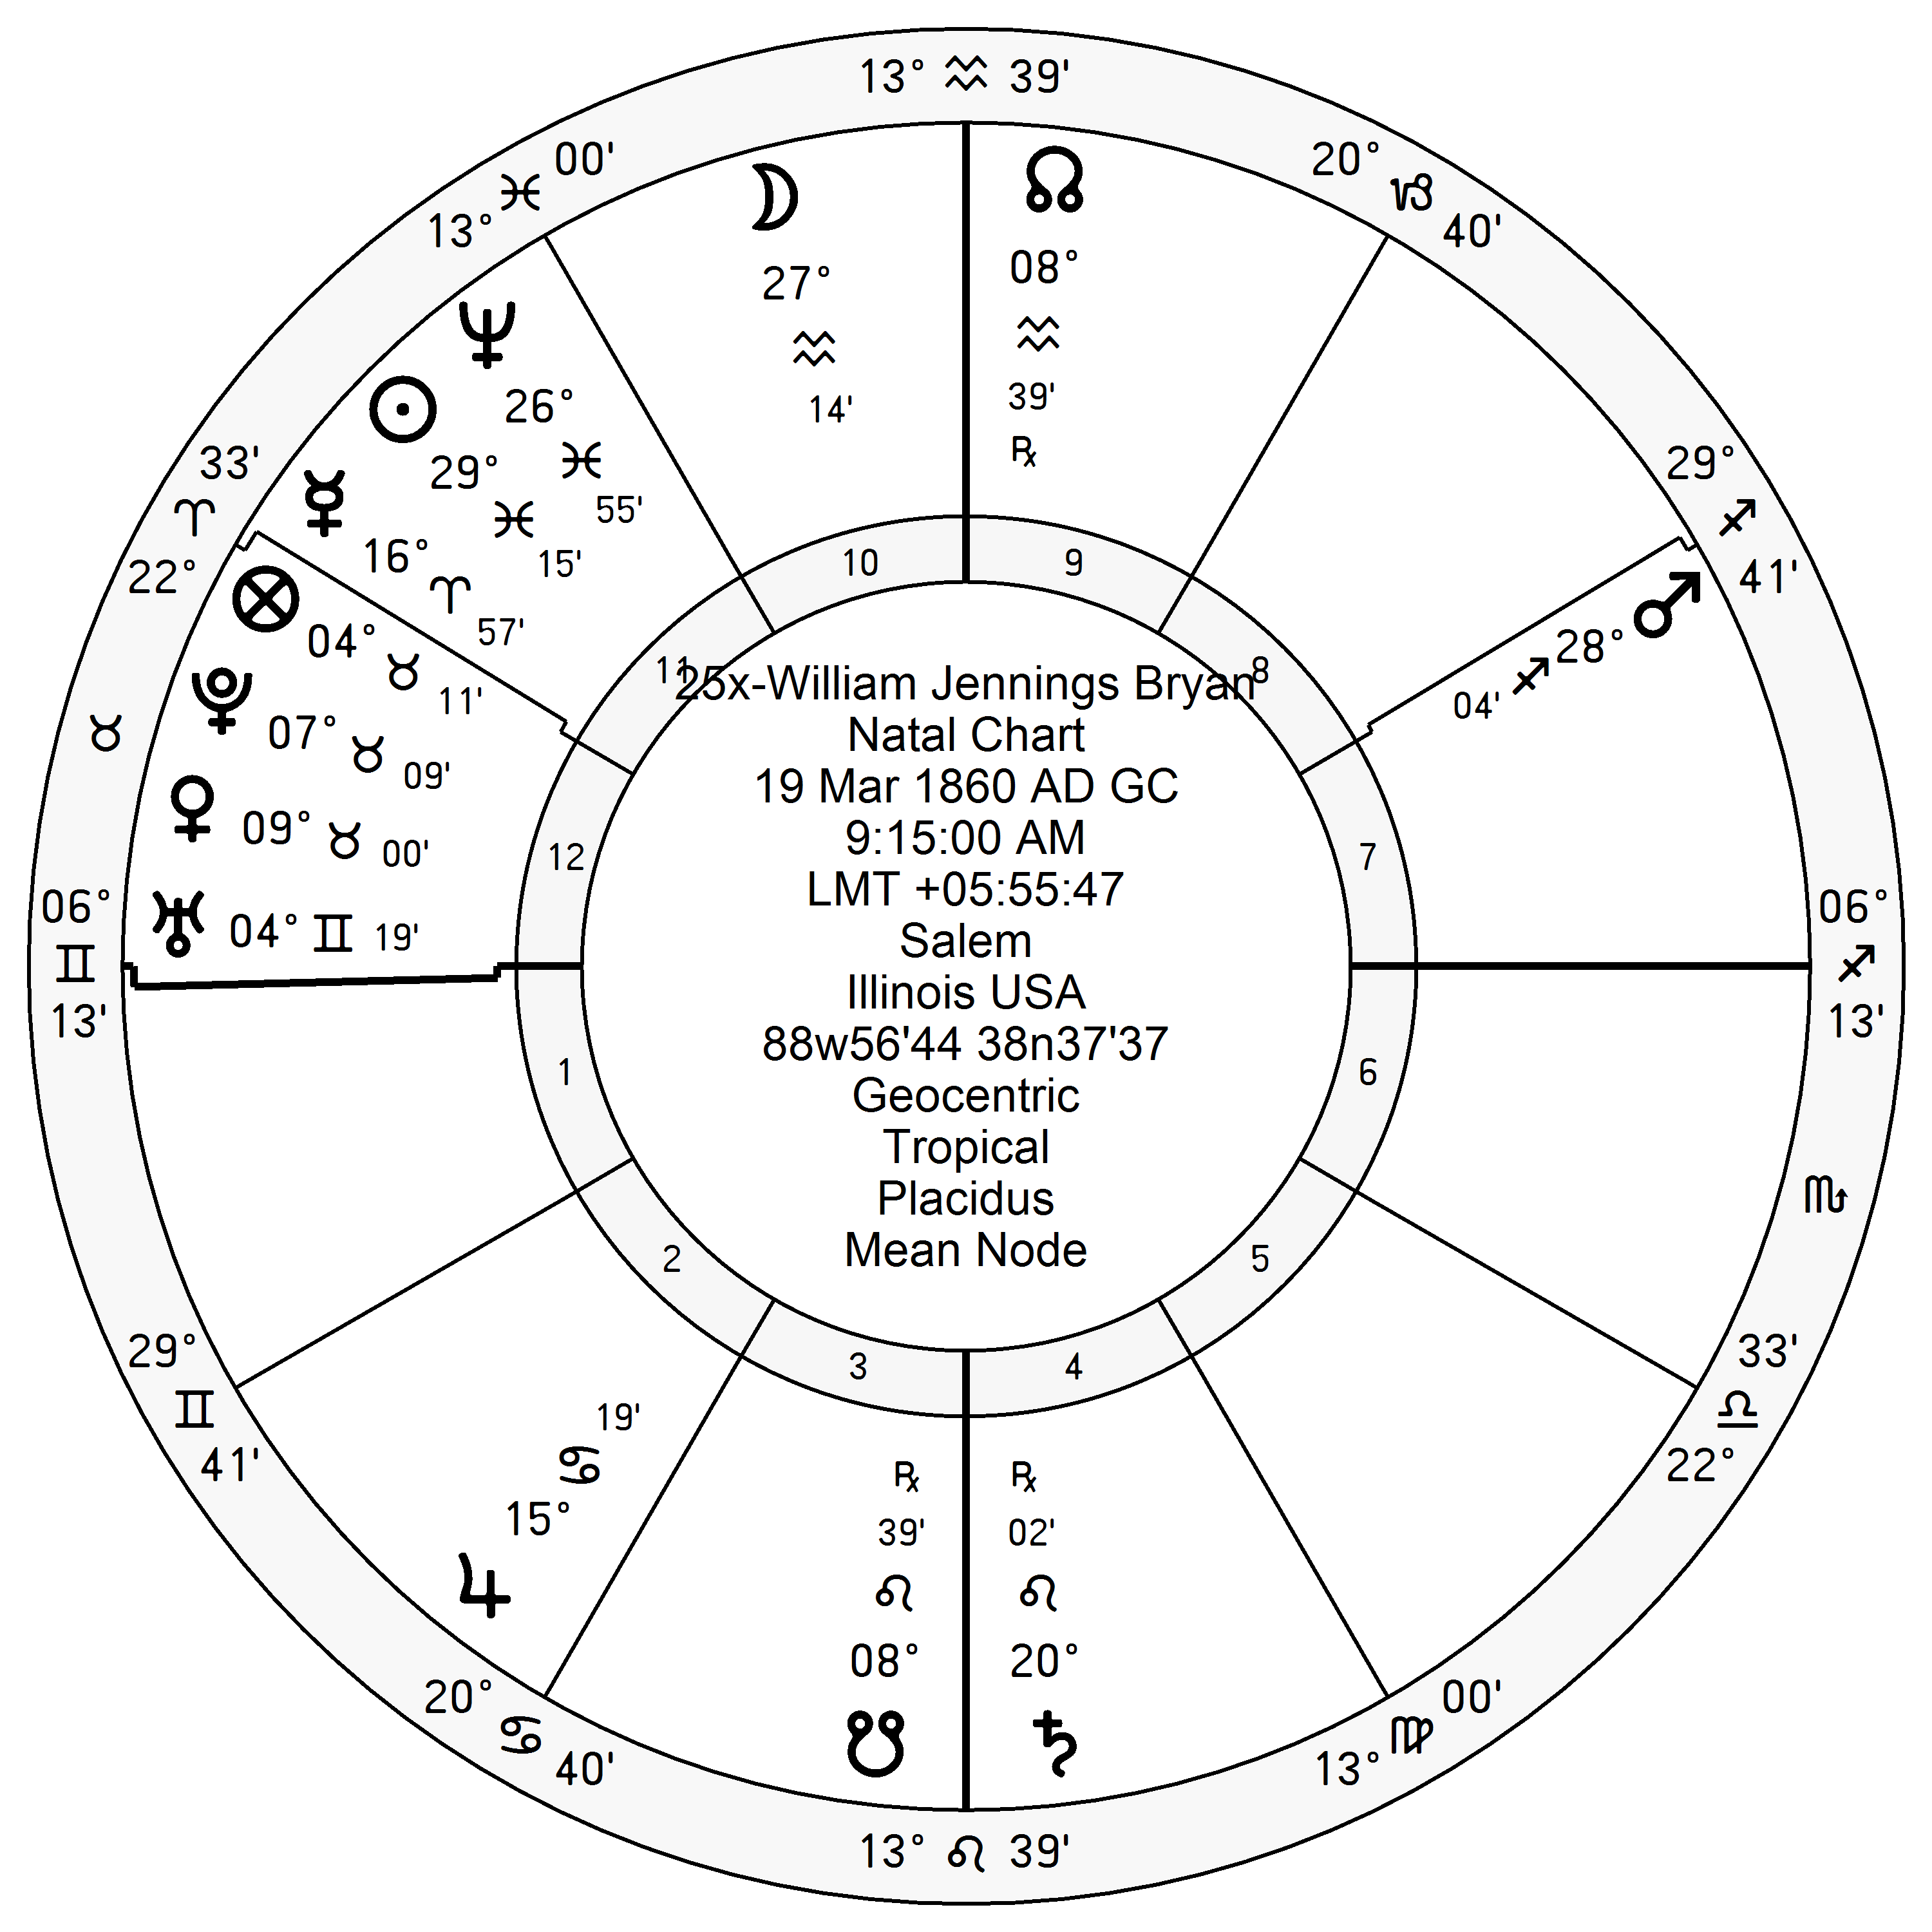
\includegraphics[width=0.9\textwidth]{charts/Bryan.png}}
\fontsize{8pt}{9pt}\selectfont

\Venus\, \Sextile\, P10, N10 \\
\Moon\, in N10, \Trine\, N1 \\
\Saturn\, \Opposition\, N10.

\column{0.48\textwidth}
\vspace{-1em}
{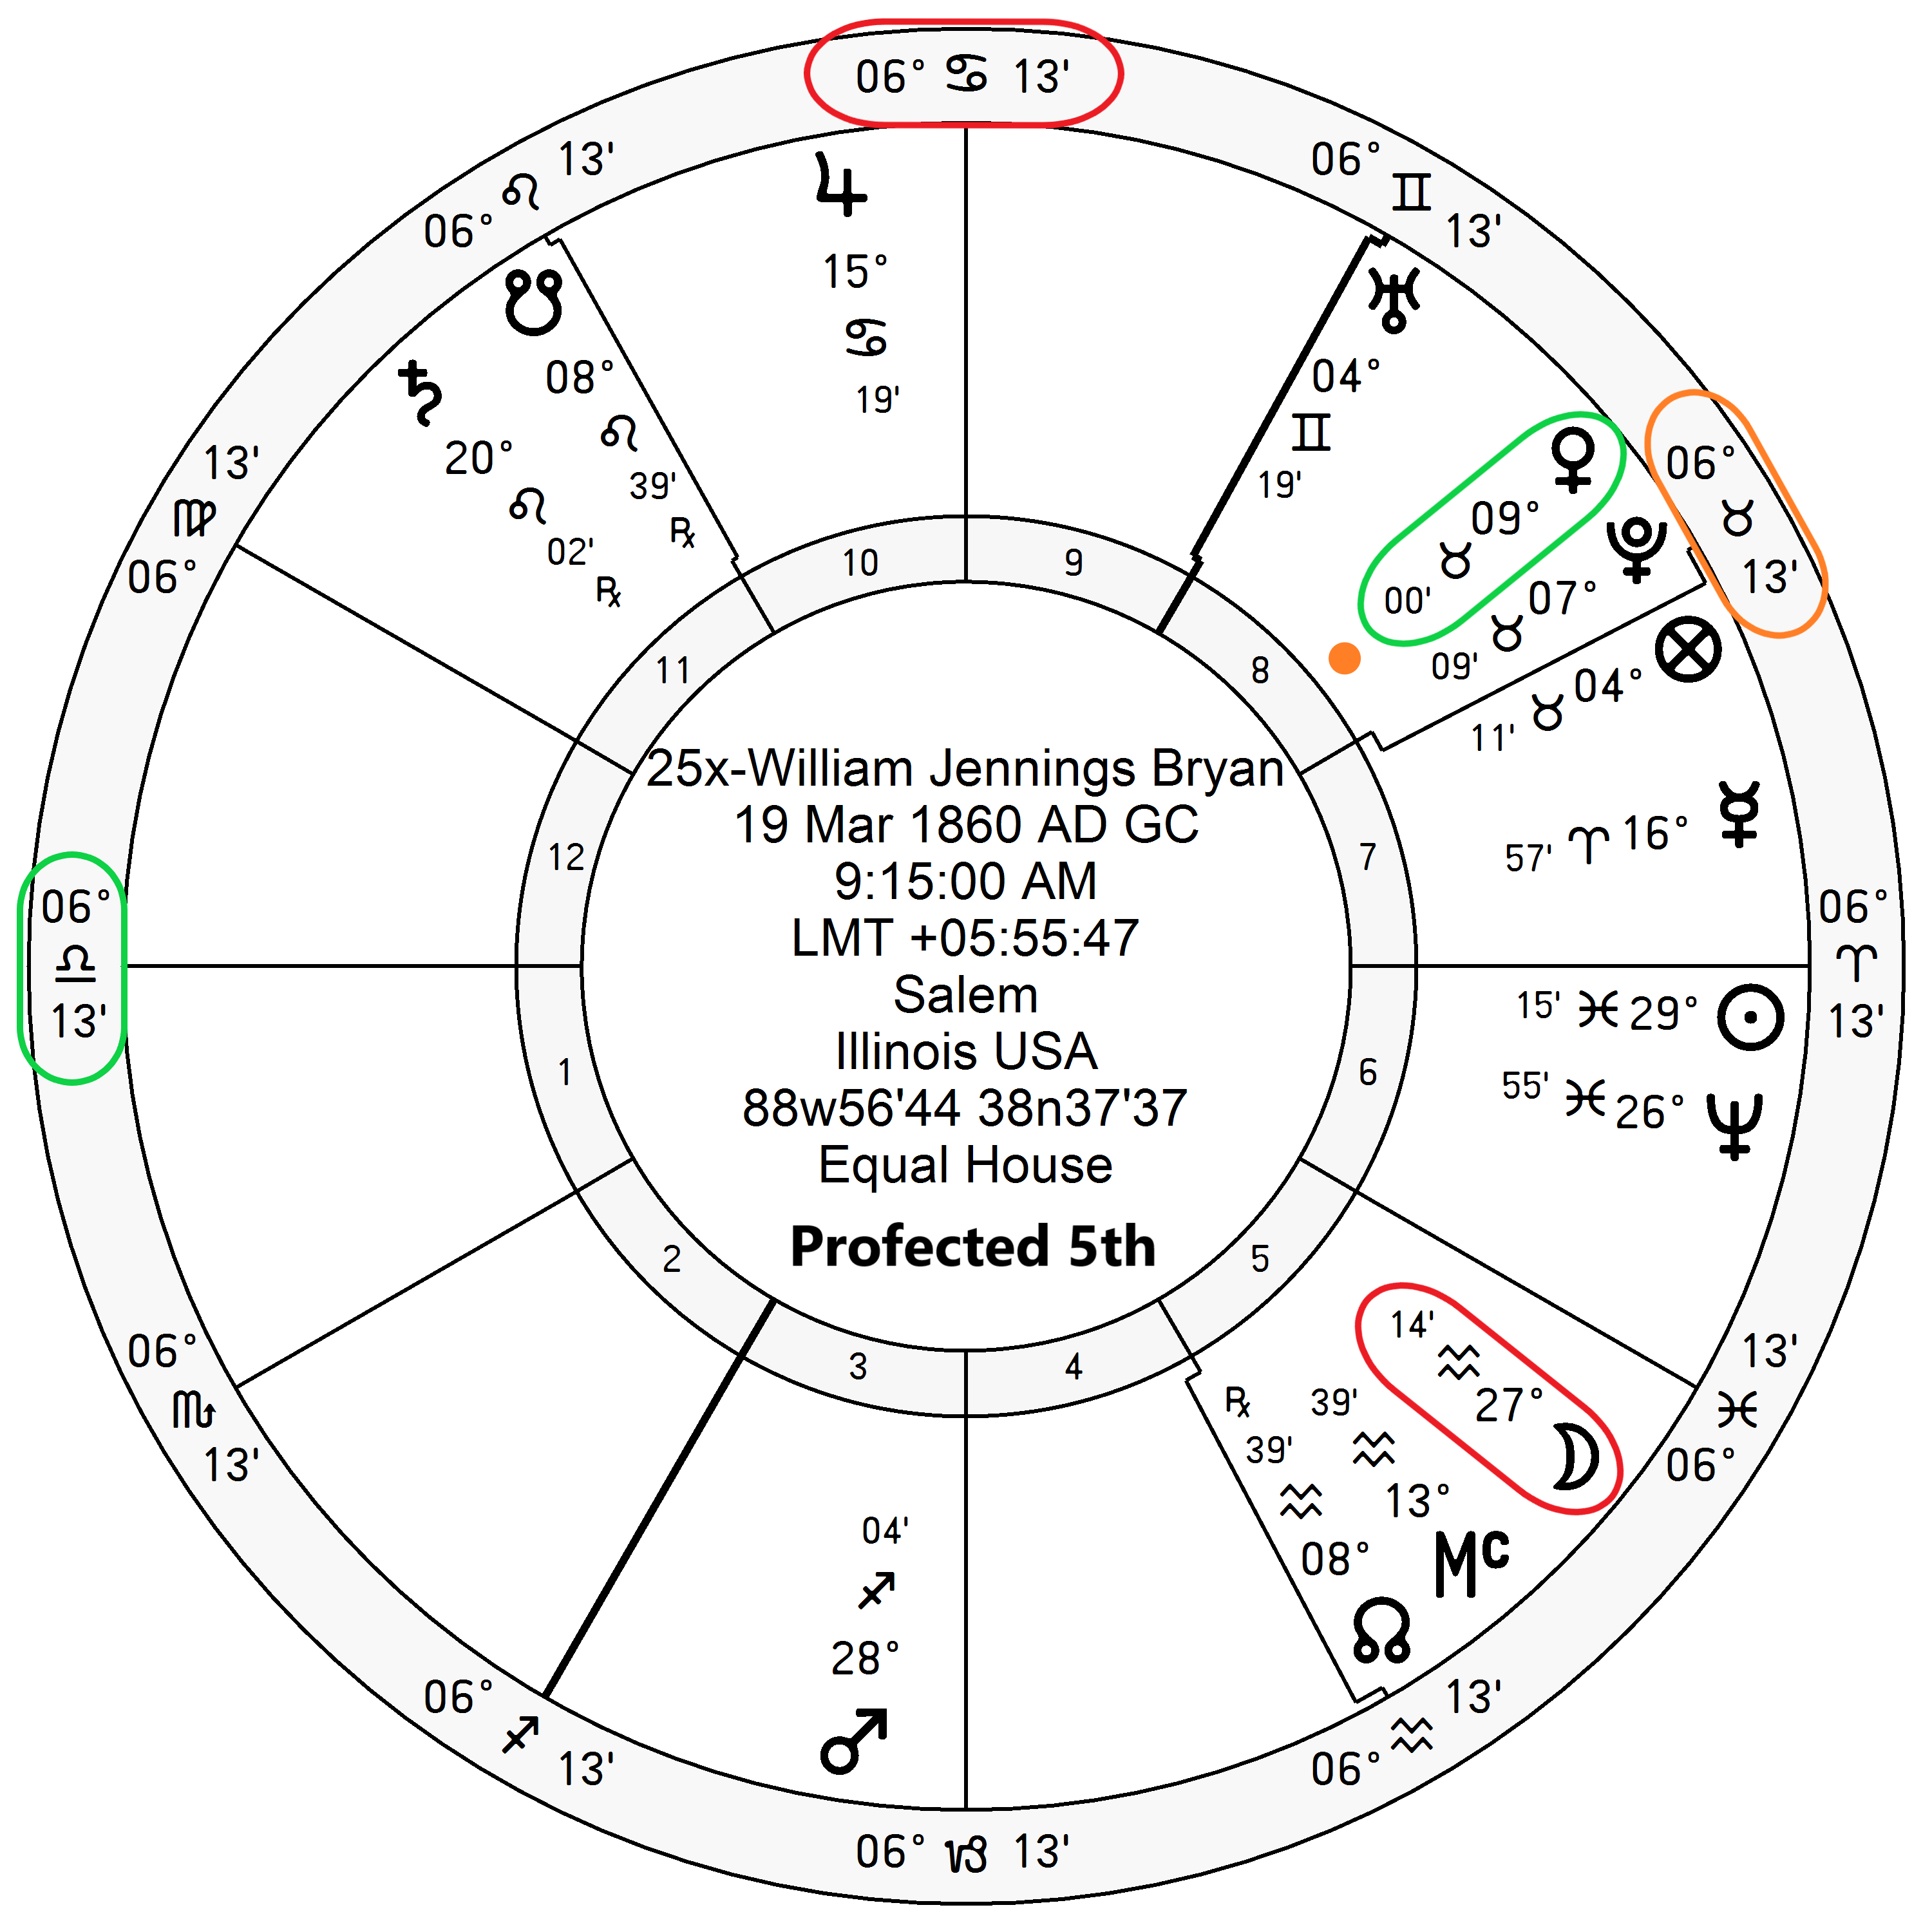
\includegraphics[width=0.9\textwidth]{charts/Bryan-Prof-5th.png}}
\textbf{\dgreen P1}=N6 
	$\Rightarrow$ \Venus\, $\Rightarrow$ \textbf{\dgreen P8/N12}\\
\textbf{\red P10}=N3
	$\Rightarrow$ \Moon\, $\Rightarrow$ P5/\textbf{\red N10}\\
PE=\textbf{\dgreen P8/N12}
	$\Rightarrow$ \Saturn\,\Retrograde $\Rightarrow$ \textbf{\dgreen P8/N12}

\end{columns}
\end{frame}

%\subsection{Election November 3, 1908: *Taft vs Bryan}
\begin{frame}[t]{Election November 3, 1908: *William Taft}
\small
% Taft
\begin{columns}[T, onlytextwidth]
\column{0.48\textwidth}
\vspace{-1em}
{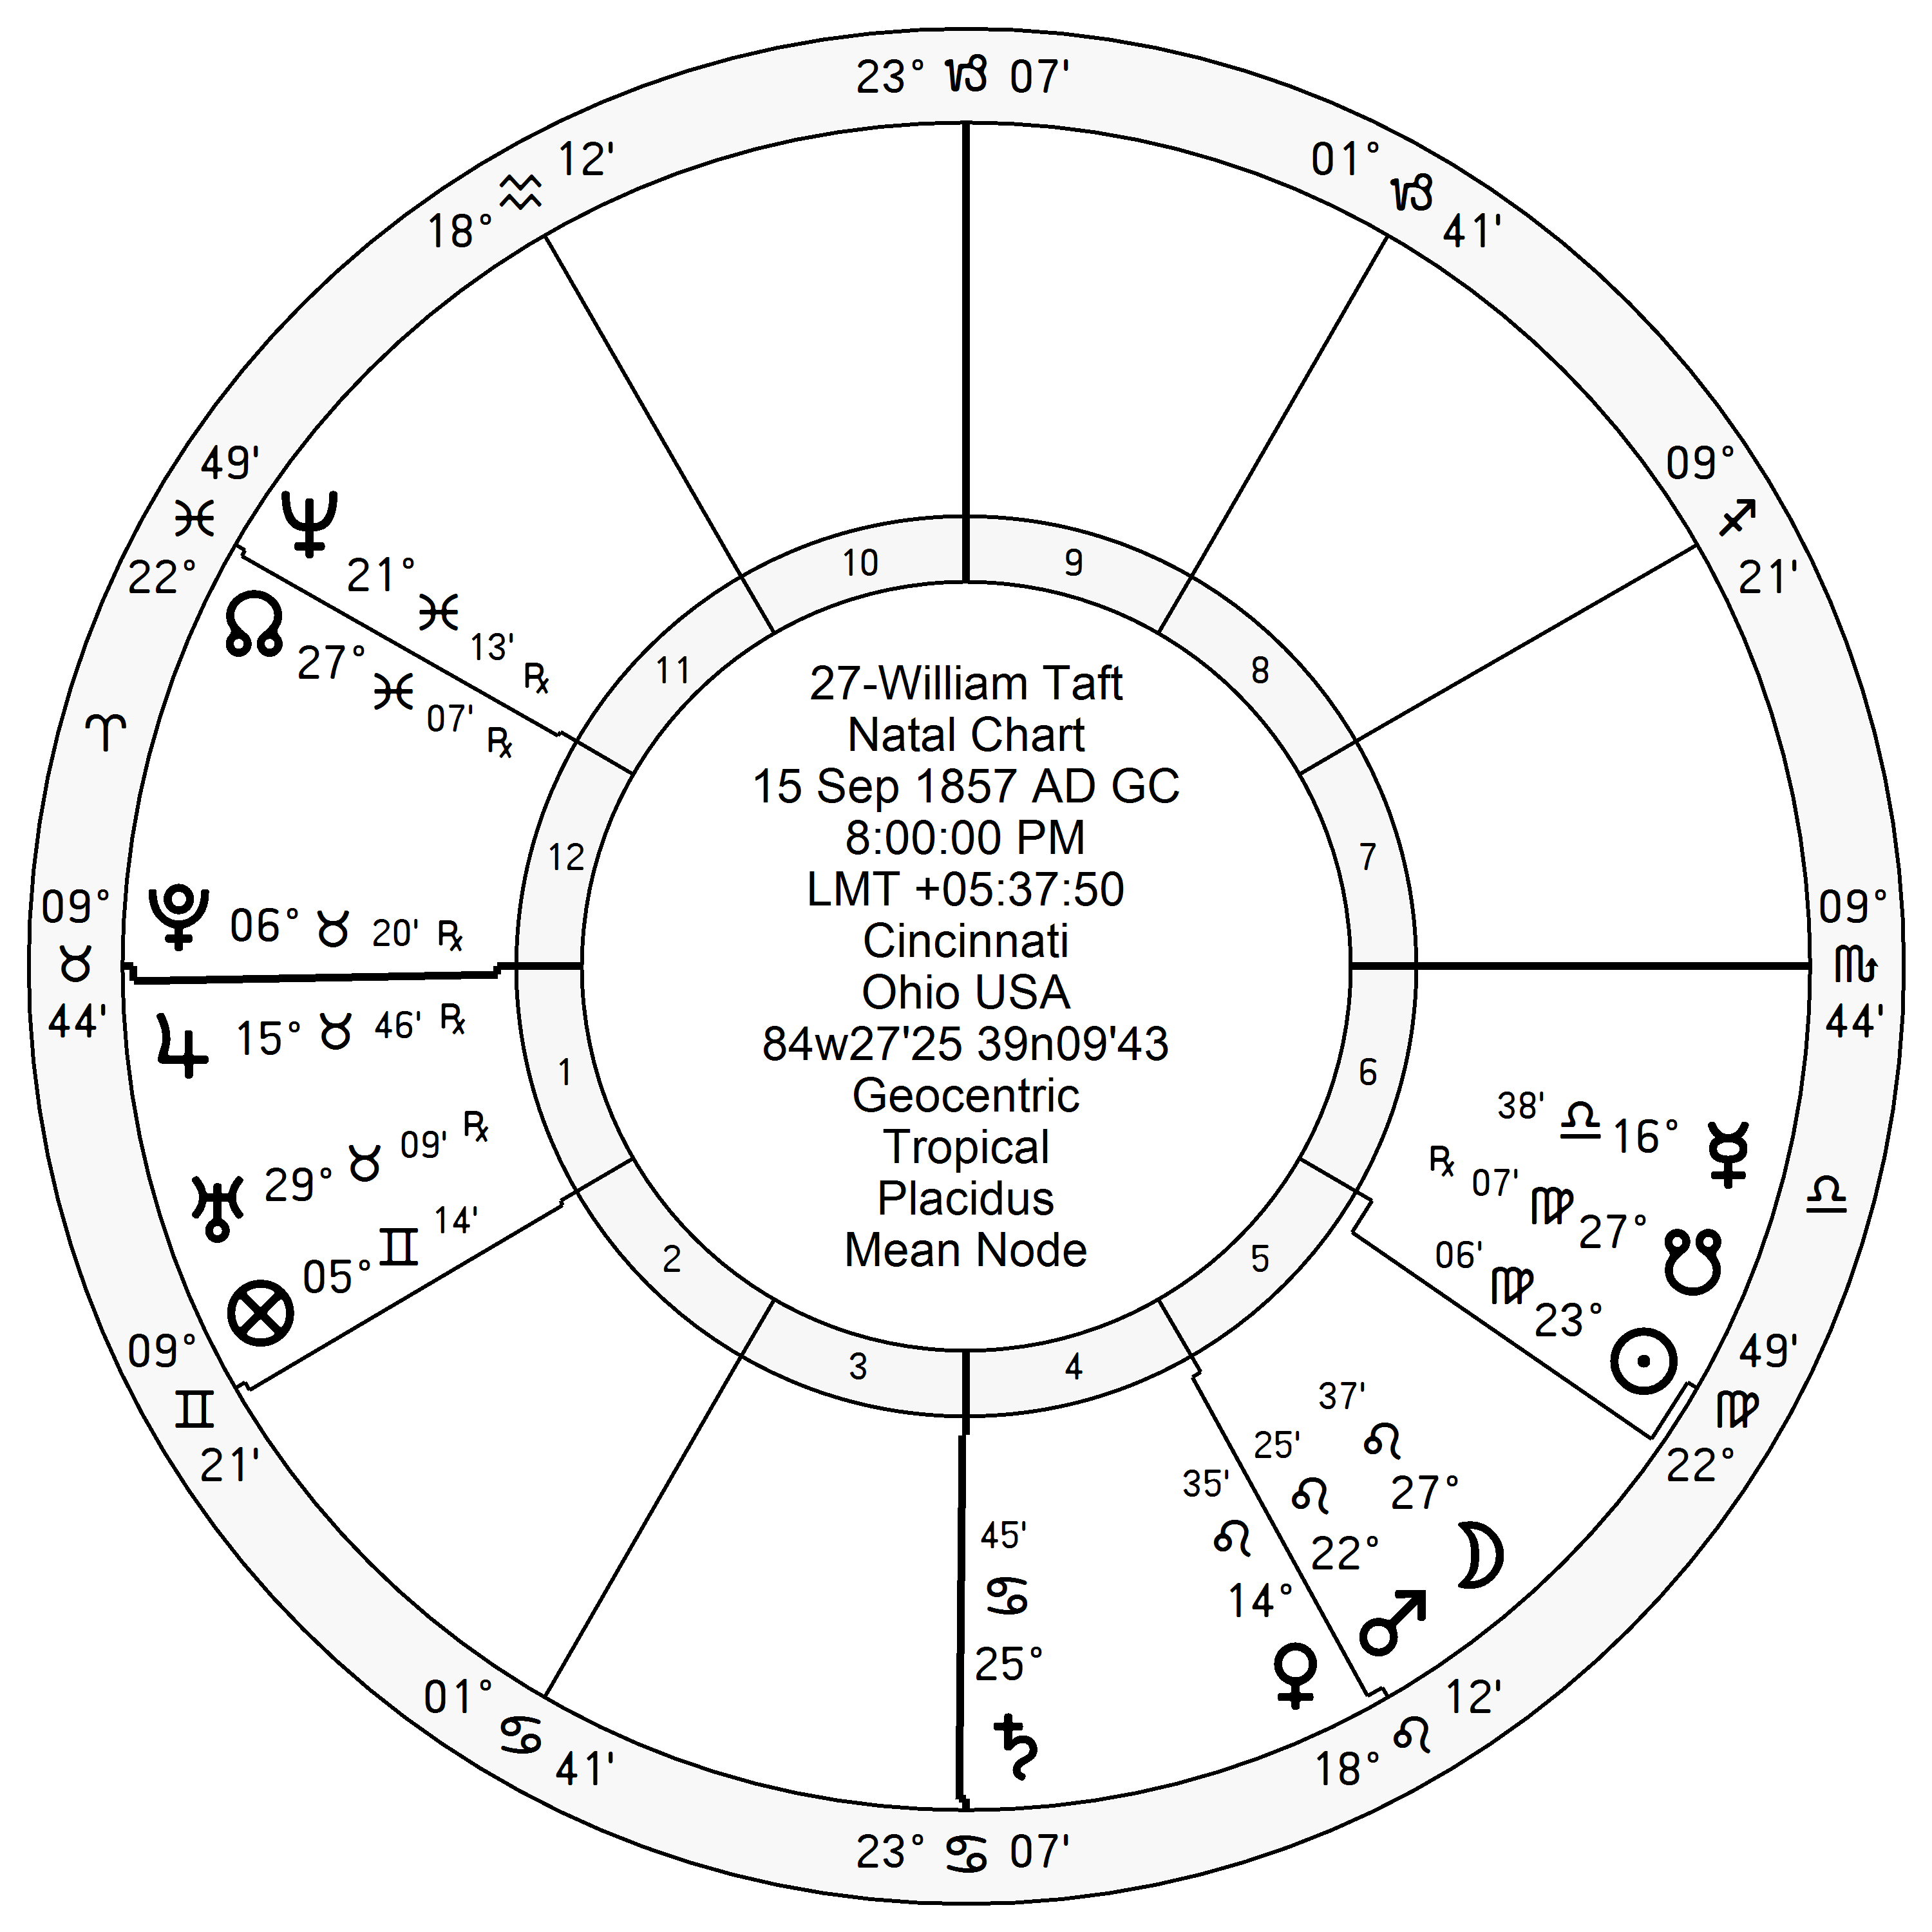
\includegraphics[width=0.9\textwidth]{charts/Taft.png}}
\fontsize{7pt}{8pt}\selectfont

There are connections between P1, P10 and N1 although the underlying houses are weak it appears Bryan's were weaker and worse. The \Sun\, with the \SouthNode\, may have marked him as a one term President.

\column{0.48\textwidth}
\vspace{-1em}
{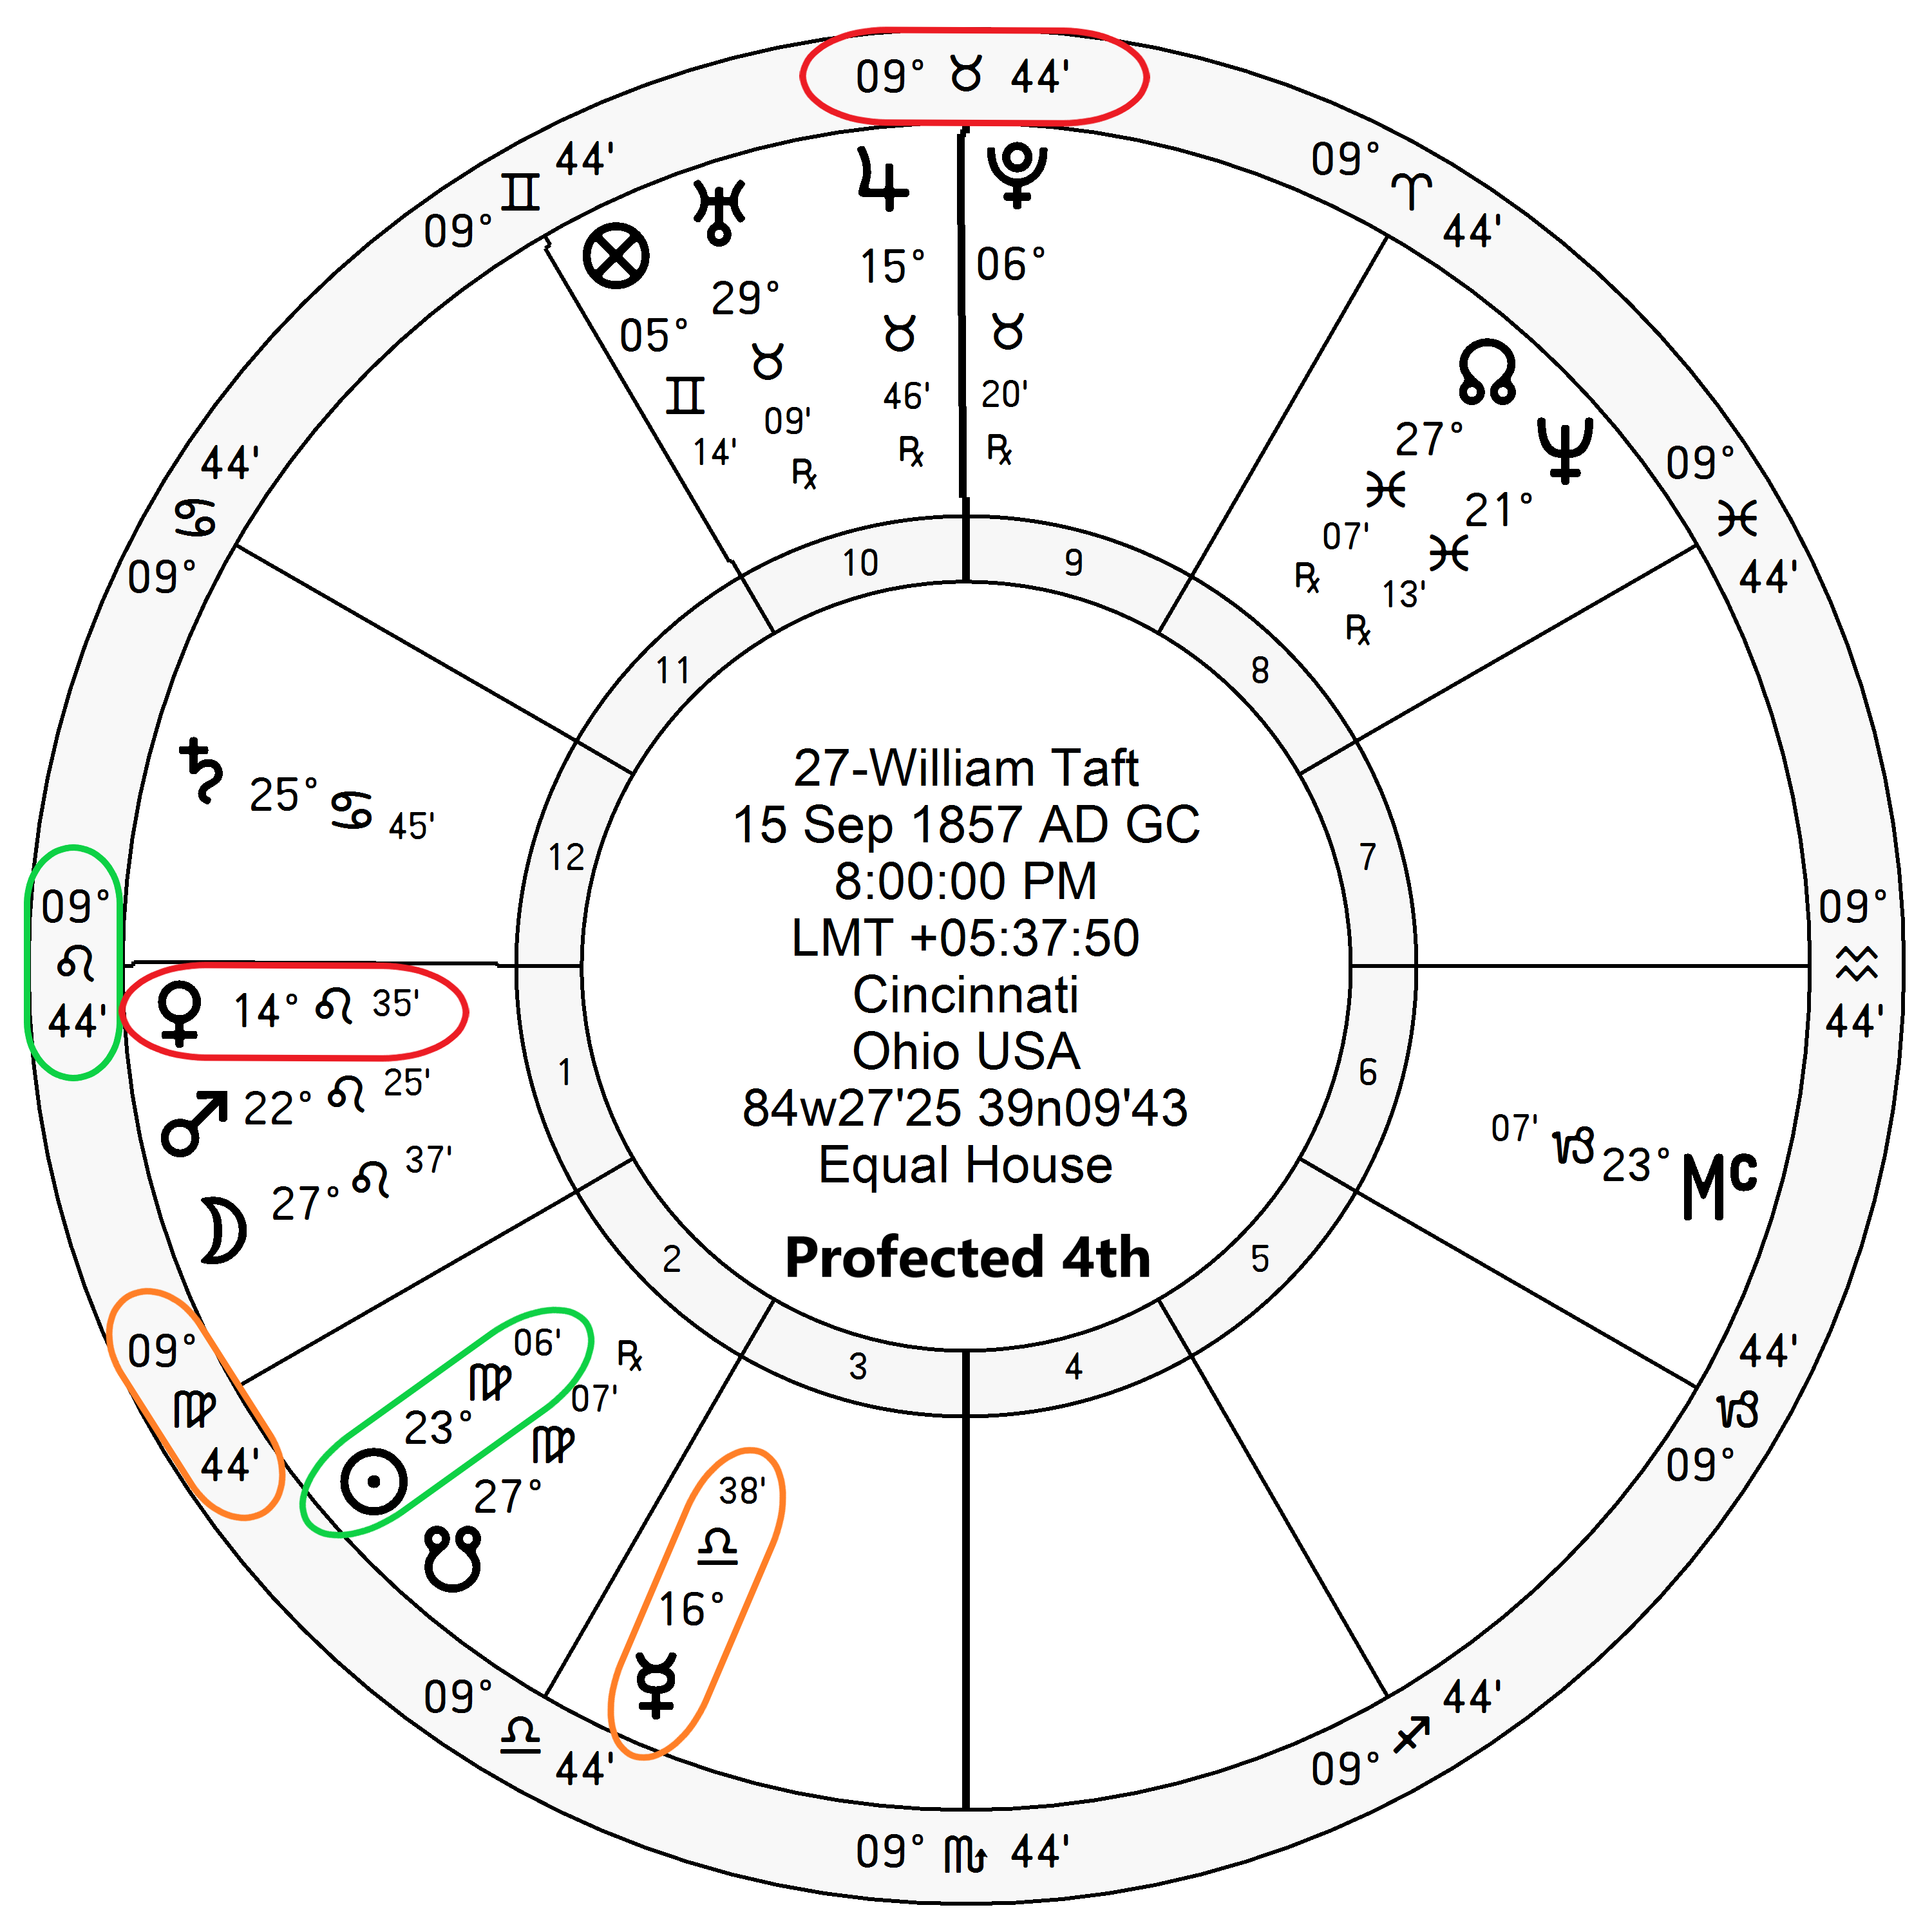
\includegraphics[width=0.9\textwidth]{charts/Taft-Prof-4th.png}}

\textbf{\dgreen P1}=N5
	$\Rightarrow$ \Sun\,\Conjunction\,\SouthNode $\Rightarrow$ \textbf{\dgreen P2/N6} \\
\textbf{\red P10=N1} 
	$\Rightarrow$  \Venus\, $\Rightarrow$  \textbf{\dgreen P1}/N4 \\
PE=\textbf{\dgreen P2/N6}
	$\Rightarrow$  \Mercury\, $\Rightarrow$  P3/\textbf{\dgreen N6}

\end{columns}
\end{frame}

% Bryan
\begin{frame}[t]{Election November 3, 1908: William Jennings Bryan}
\small
\begin{columns}[T, onlytextwidth]
\column{0.48\textwidth}
\vspace{-1em}
{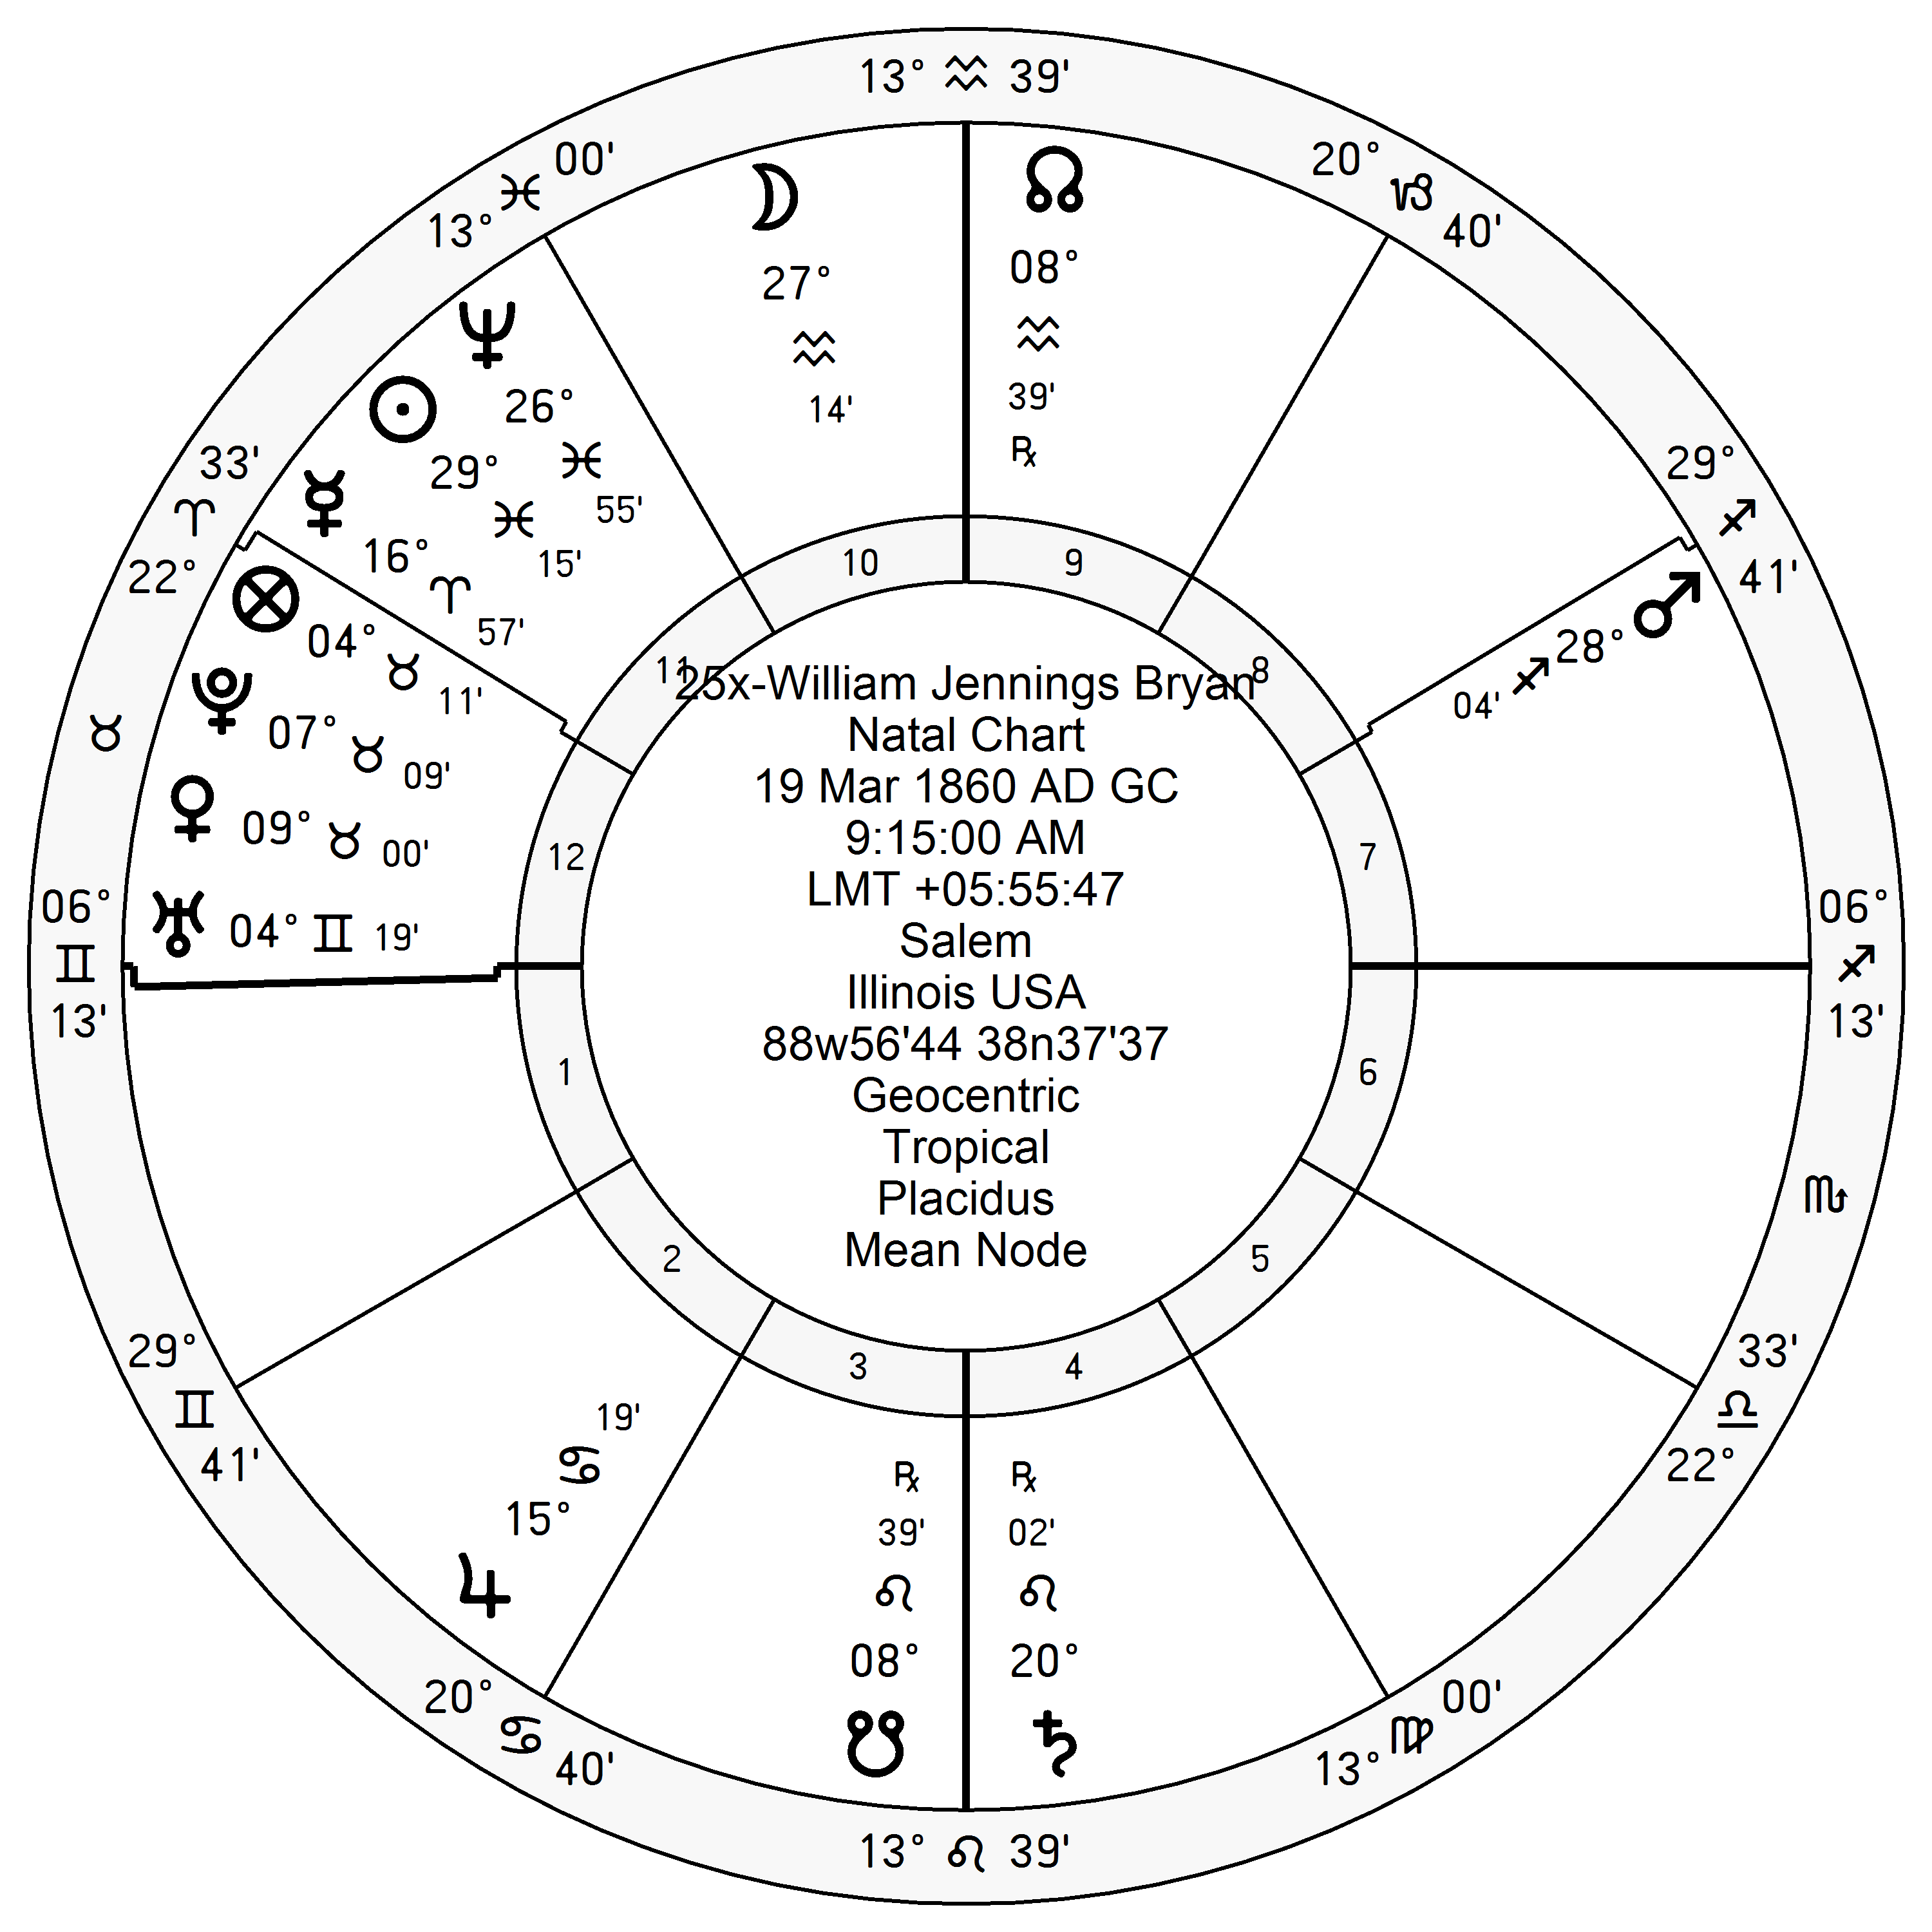
\includegraphics[width=0.9\textwidth]{charts/Bryan.png}}
\fontsize{8pt}{9pt}\selectfont

This election is 12 years to the day from the 1896 election; the setup and result are the same.

\column{0.48\textwidth}
\vspace{-1em}
{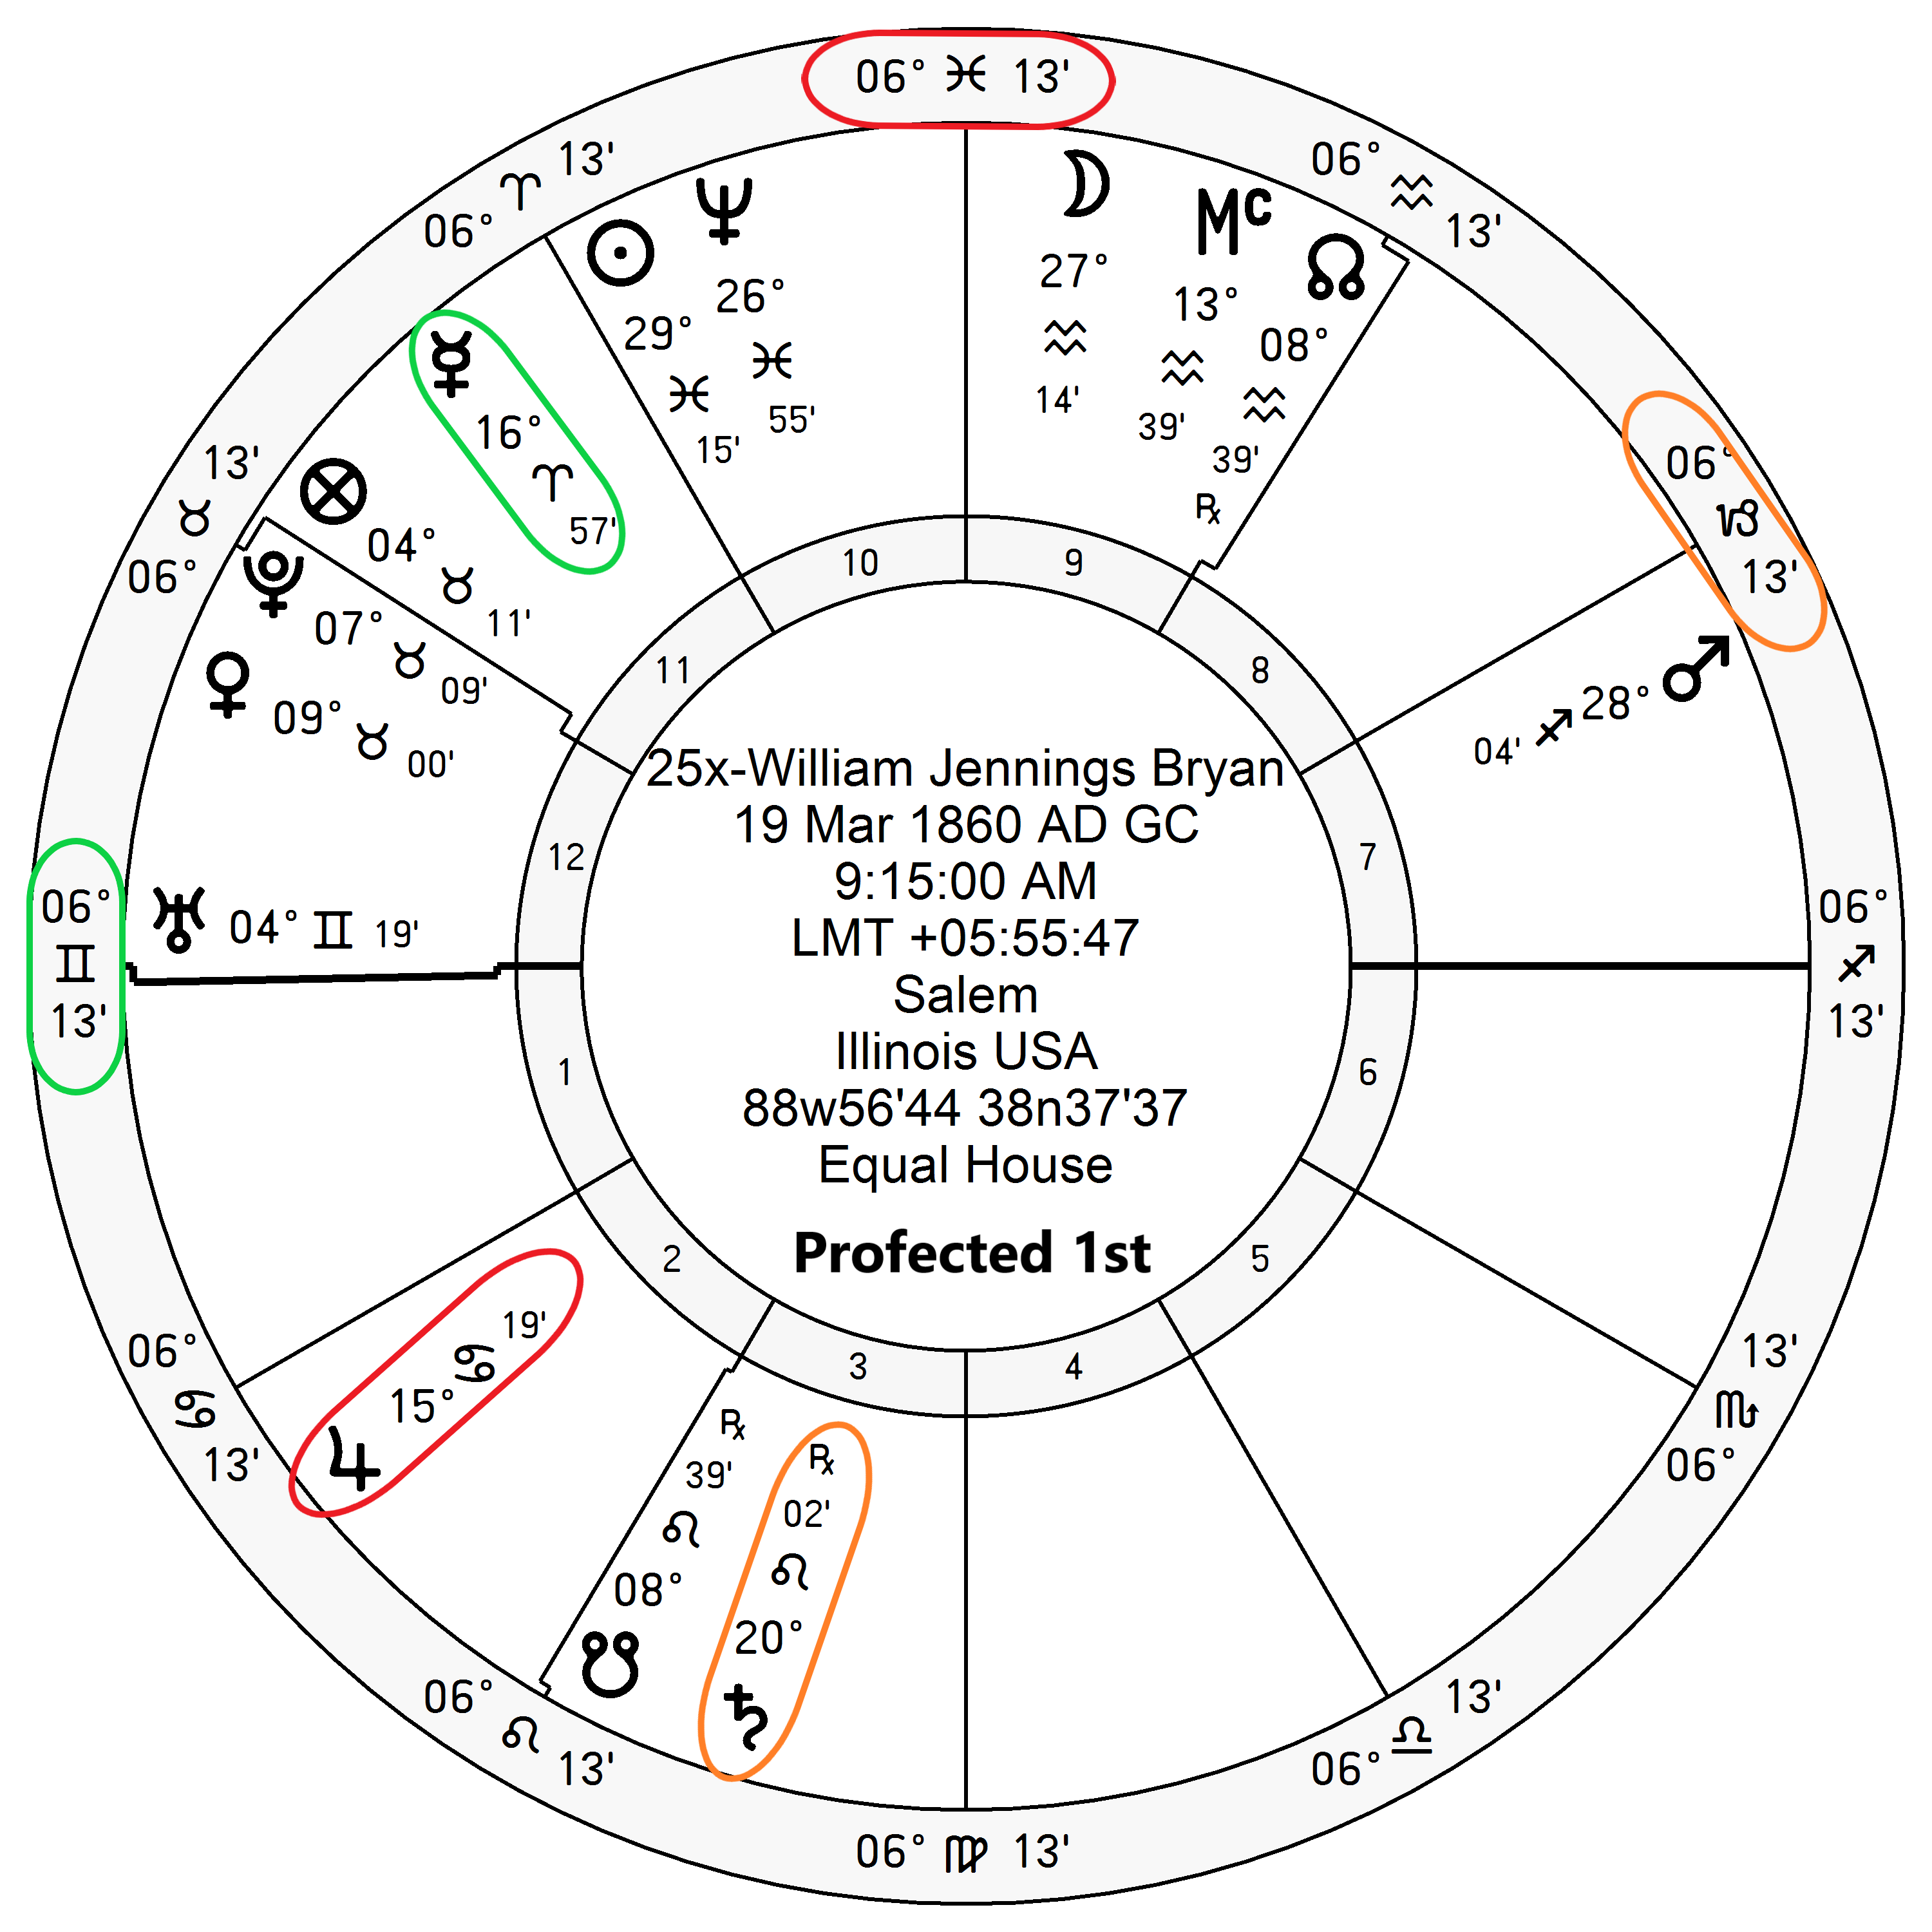
\includegraphics[width=0.9\textwidth]{charts/Bryan-Prof-1st.png}}

\textbf{\dgreen P1=N1} 
	$\Rightarrow$ \Mercury\, $\Rightarrow$ P11/N11\\
\textbf{\red P10=N10}
	$\Rightarrow$ \Jupiter\, $\Rightarrow$ P2/N2\\
PE=P8/N8 
	$\Rightarrow$ \Saturn\,\Retrograde $\Rightarrow$ P3/N4


\end{columns}
\end{frame}

%\subsection{Election November 5, 1912: *Wilson vs Roosevelt}
\begin{frame}[t]{Election November 5, 1912: *Woodrow Wilson}
\small
% Wilson
\begin{columns}[T, onlytextwidth]
\column{0.48\textwidth}
\vspace{-1em}
{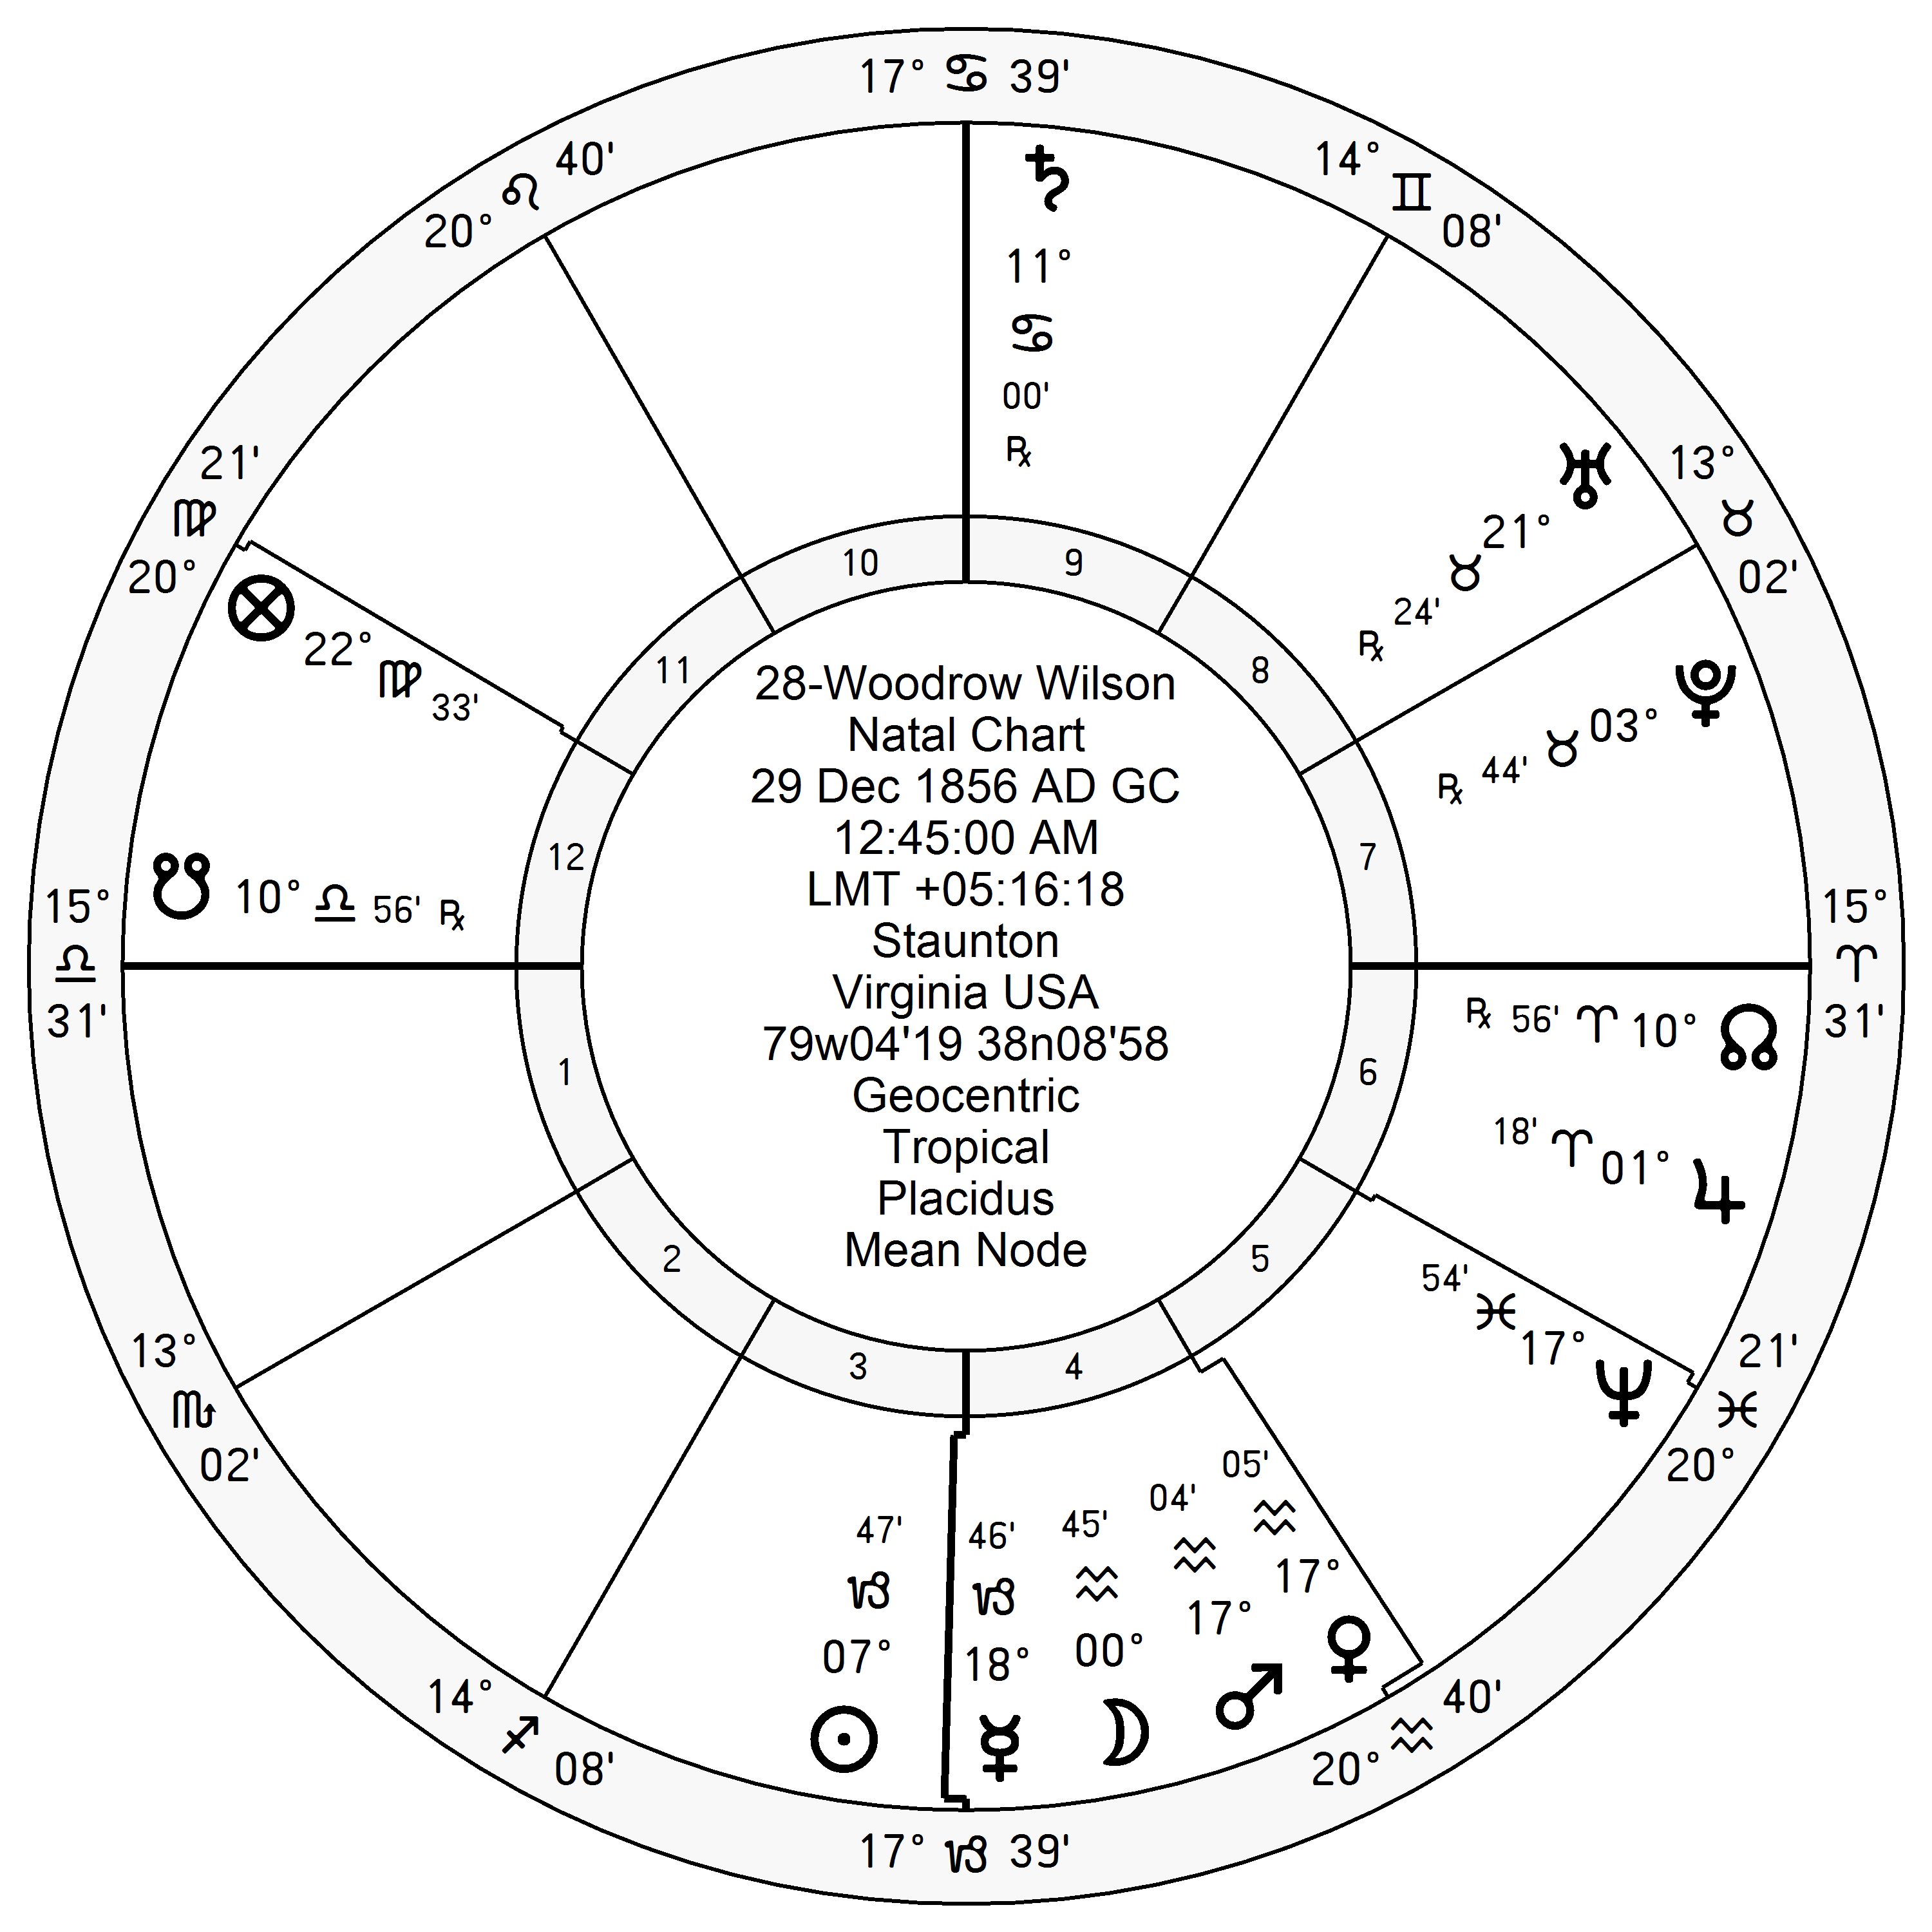
\includegraphics[width=0.9\textwidth]{charts/Wilson.png}}
\fontsize{7pt}{8pt}\selectfont

\Venus\, in P10, \Opposition\, N10; \Square\, P1, \Trine\, N1 \\
\Saturn\, \Trine\, P10 \\
\Jupiter\, makes no aspects to P1, N1 or P10, N10

\column{0.48\textwidth}
\vspace{-1em}
{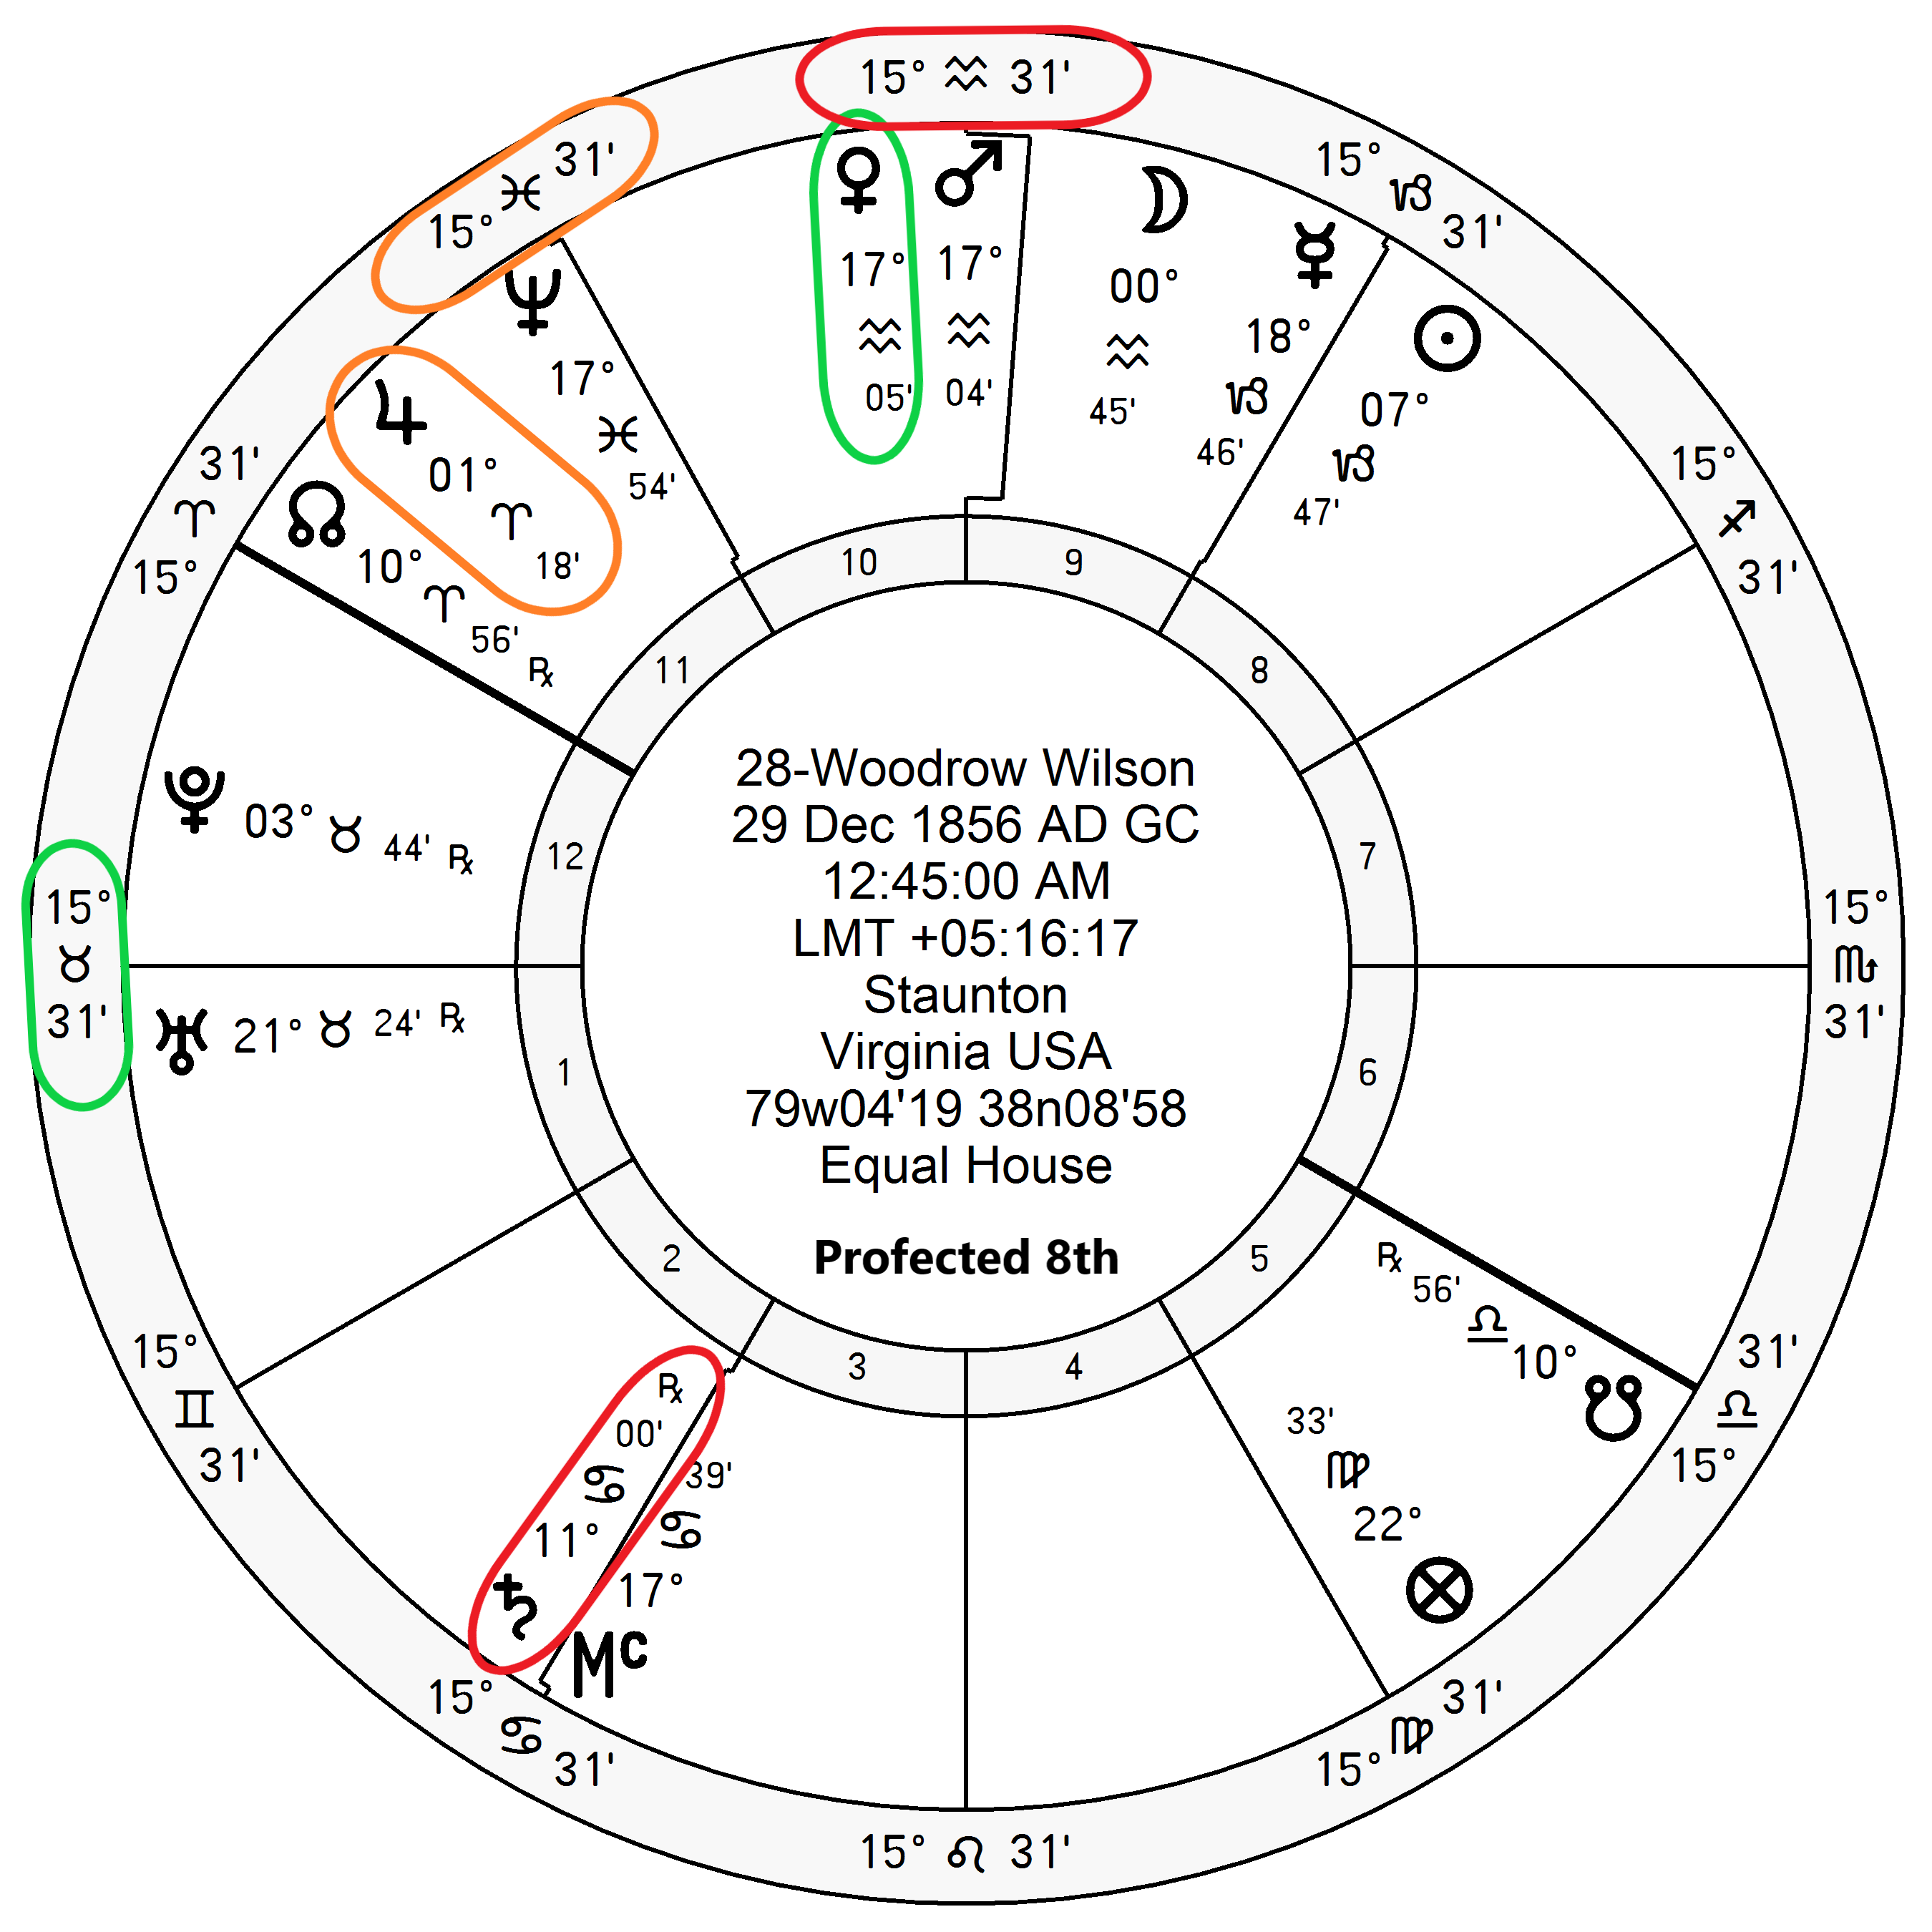
\includegraphics[width=0.9\textwidth]{charts/Wilson-Prof-8th.png}}

\textbf{\dgreen P1}=N8
	$\Rightarrow$ \Venus\, $\Rightarrow$ \textbf{\red P10}/N4 \\
\textbf{\red P10}=N5
	$\Rightarrow$  \Saturn\,\Retrograde $\Rightarrow$ P2/N9 \\
PE=P11/N6
	$\Rightarrow$  \Jupiter\, $\Rightarrow$  P11/N6

\end{columns}
\end{frame}

% Roosevelt
\begin{frame}[t]{Election November 5, 1912: Teddy Roosevelt}
\small
\begin{columns}[T, onlytextwidth]
\column{0.48\textwidth}
\vspace{-1em}
{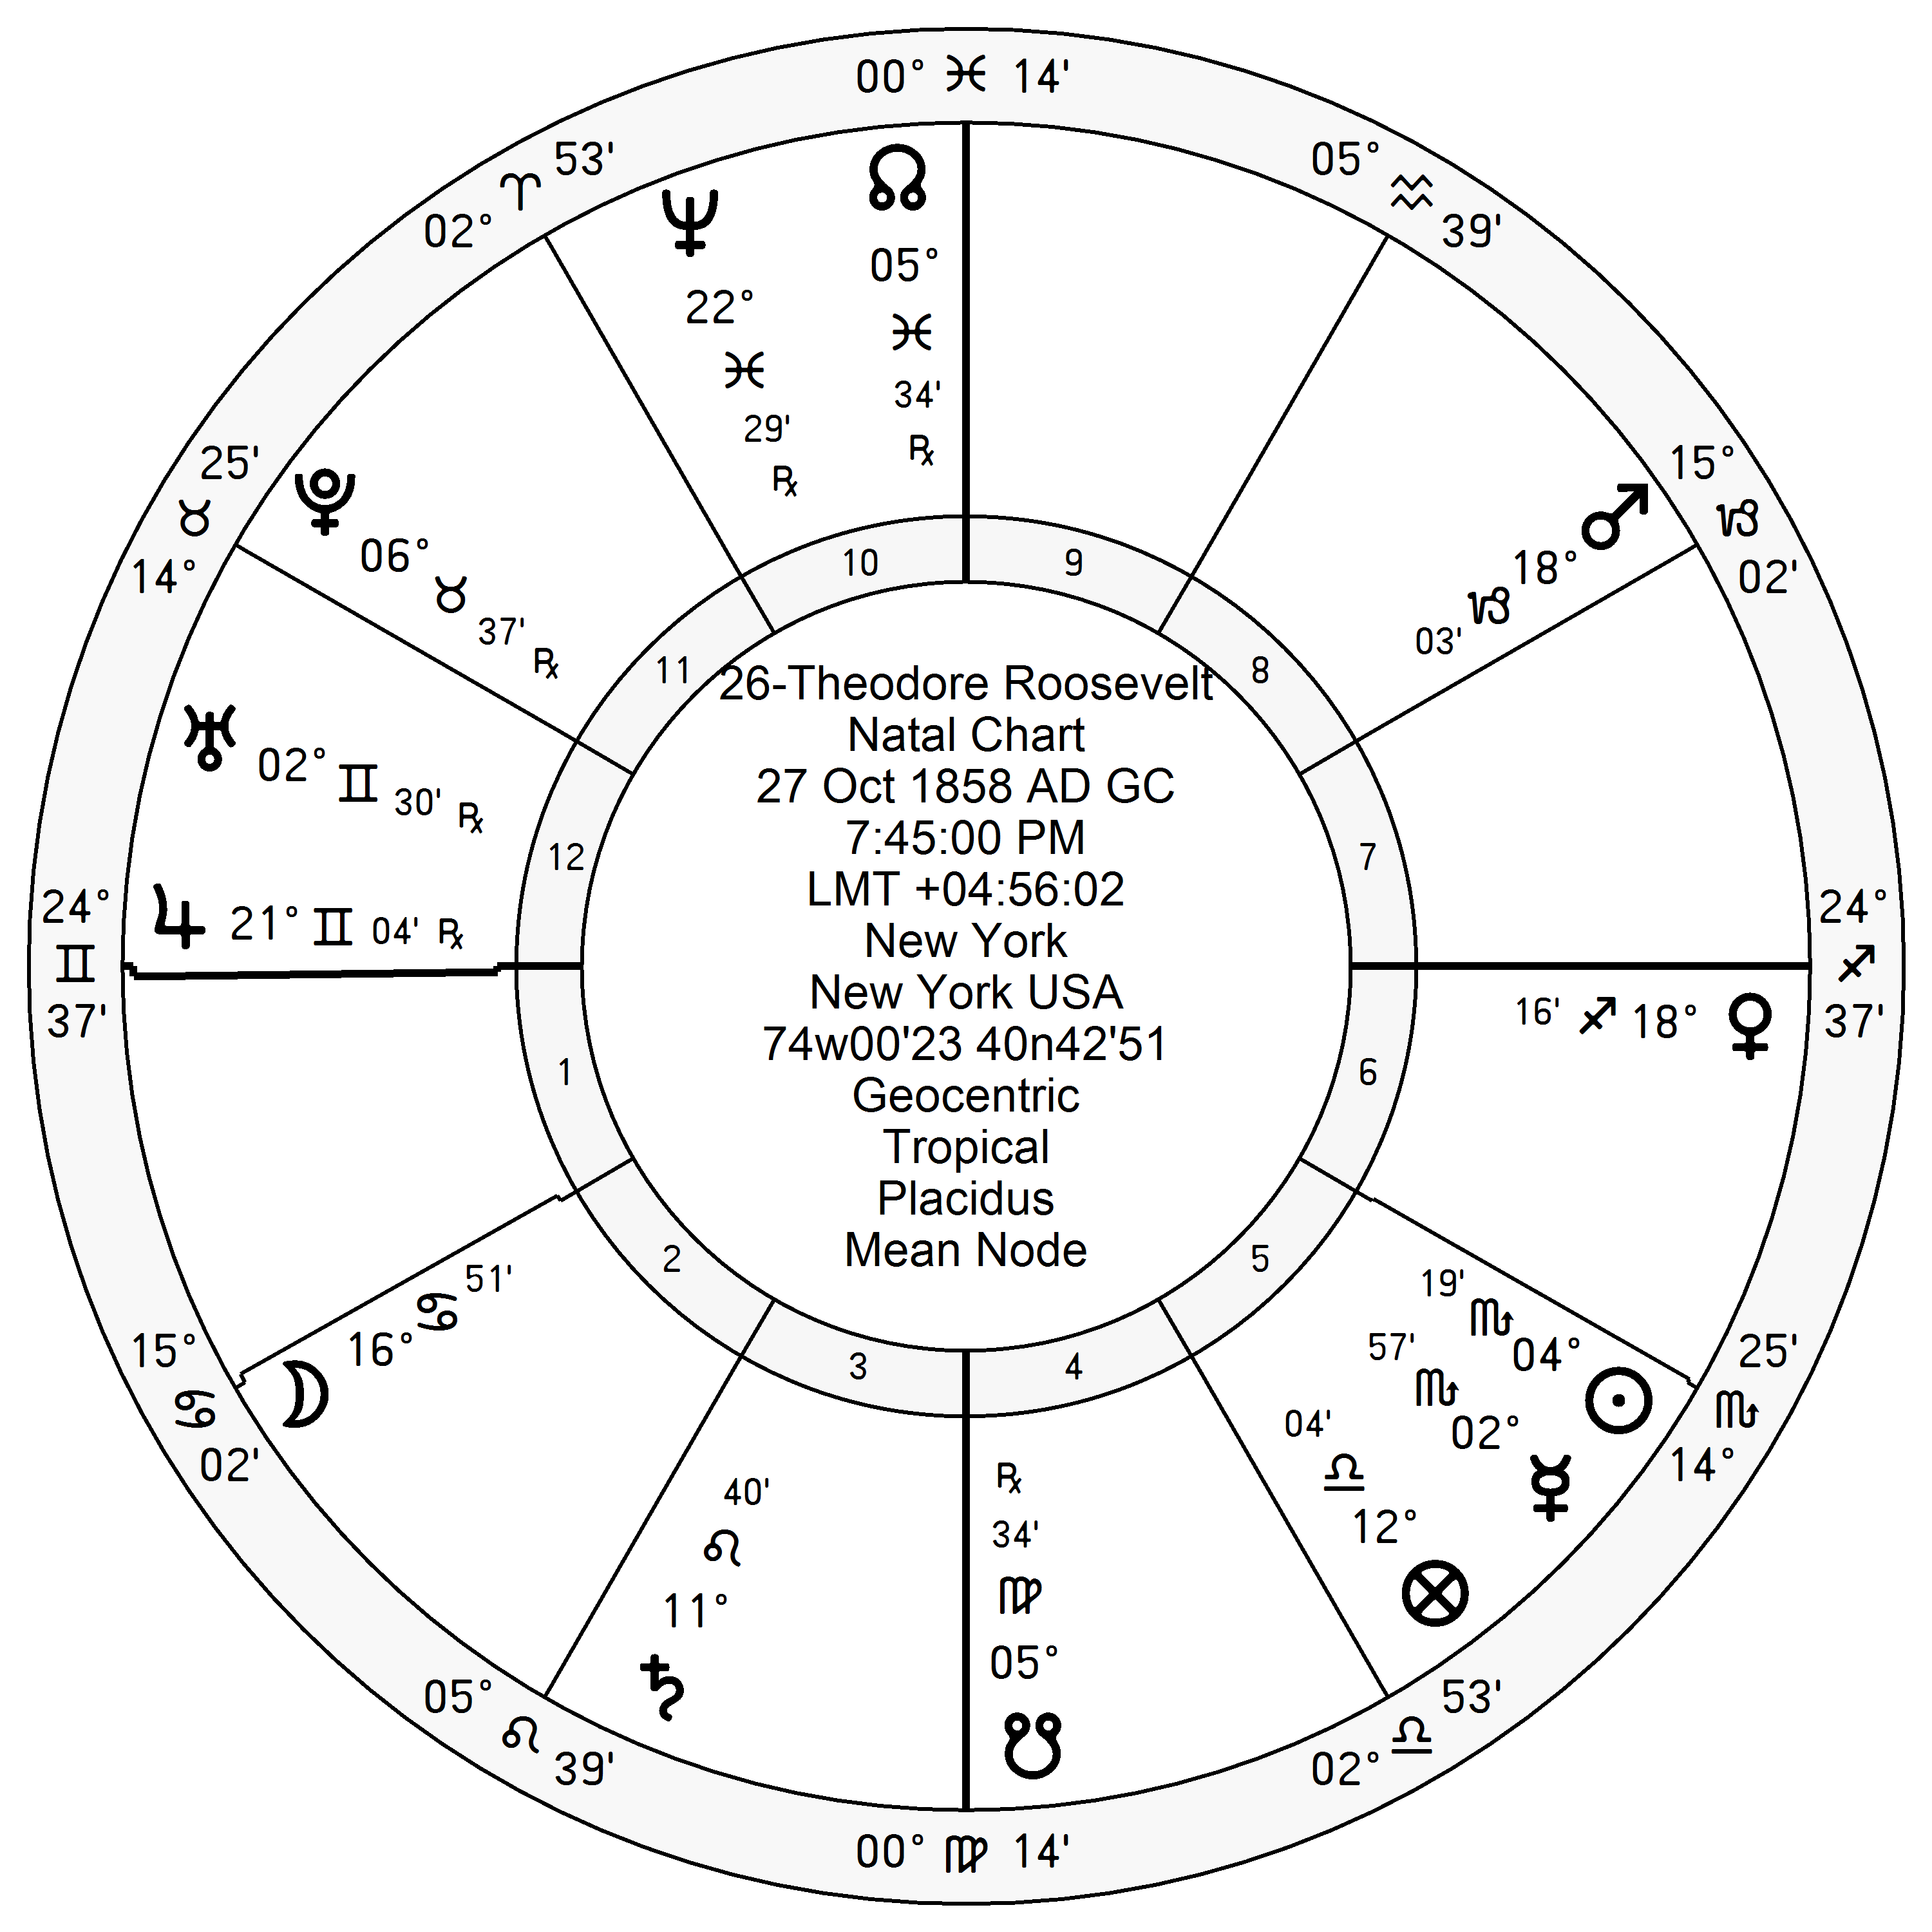
\includegraphics[width=0.9\textwidth]{charts/Roosevelt.png}}
\fontsize{8pt}{9pt}\selectfont

\Jupiter\, \Square\, N10 (1° from \Neptune) \\
\Mercury\, combust; \Trine\, N10

\column{0.48\textwidth}
\vspace{-1em}
{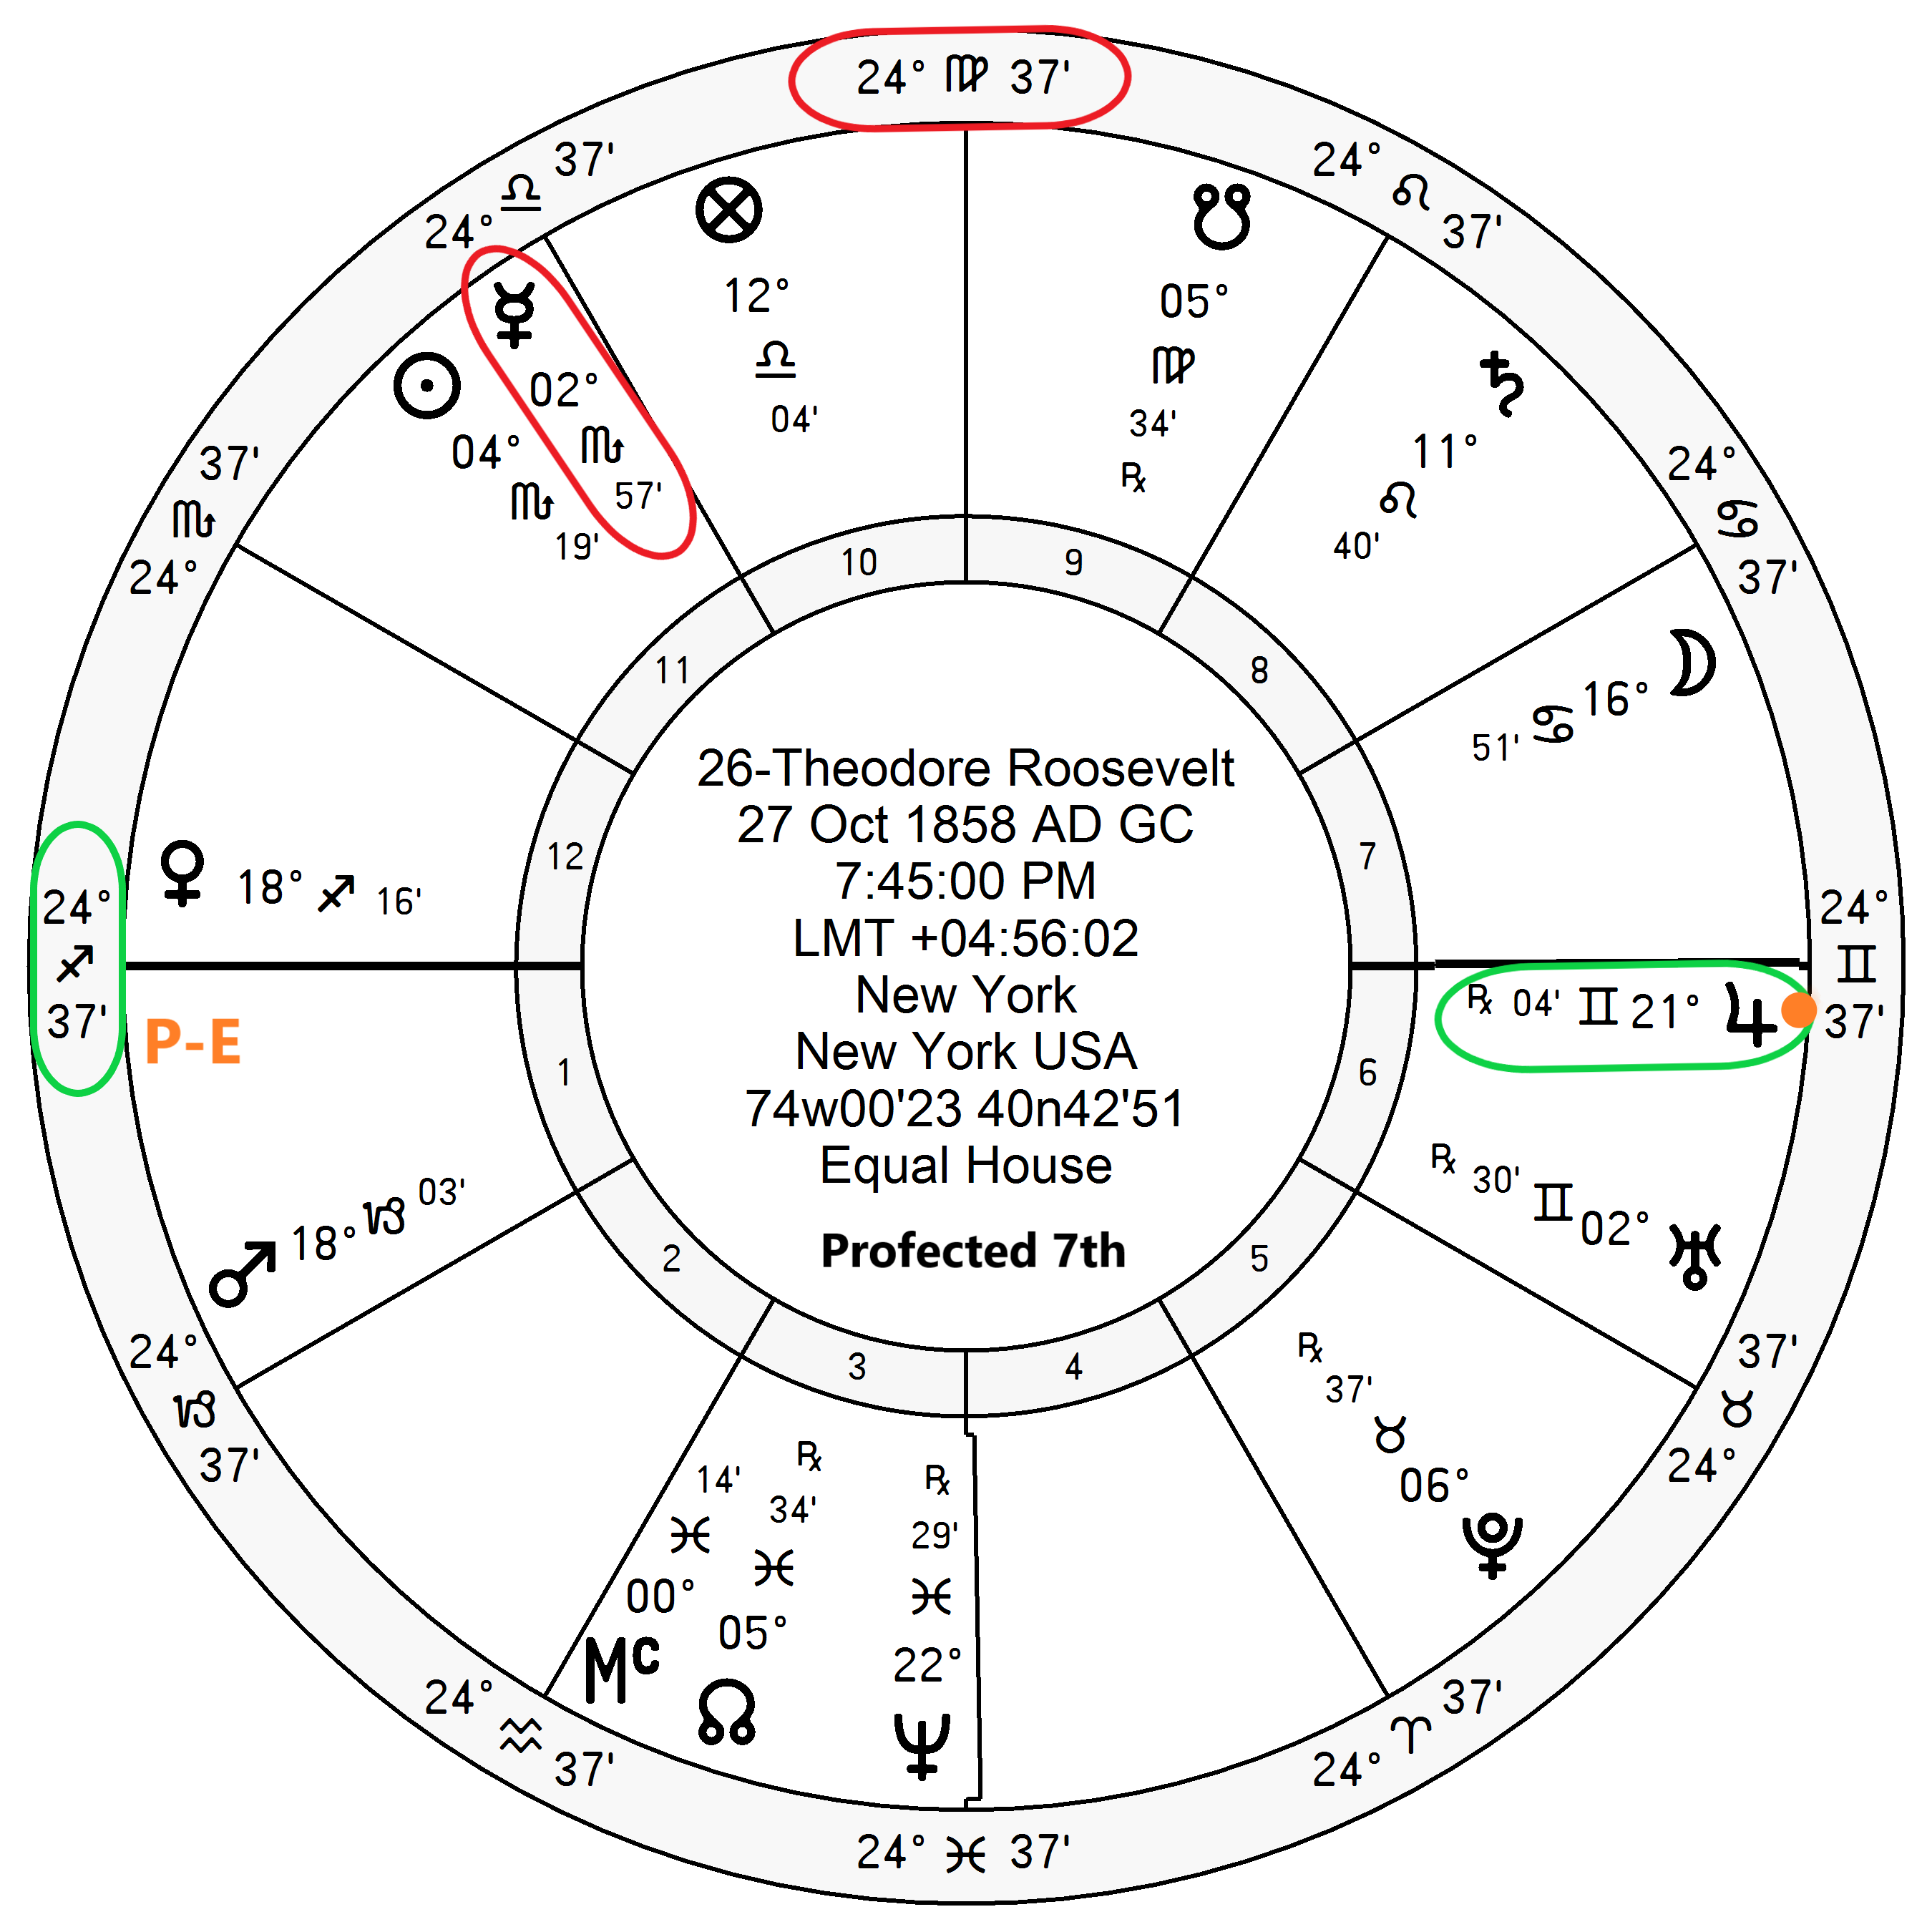
\includegraphics[width=0.9\textwidth]{charts/Roosevelt-Prof-7th.png}}
\textbf{\dgreen P1=N7} 
	$\Rightarrow$ \Jupiter\,\Retrograde $\Rightarrow$ \textbf{\dgreen P6/N12}\\
\textbf{\red P10}=N4
	$\Rightarrow$ \Mercury\, (combust) $\Rightarrow$ P11/N5\\
PE=\textbf{\dgreen P1/N7}
	$\Rightarrow$ \Jupiter\,\Retrograde $\Rightarrow$ \textbf{\dgreen P6/N12}


\end{columns}
\end{frame}

%\subsection{Election November 5, 1916: *Wilson vs Hughes}
\begin{frame}[t]{Election November 7, 1916: *Woodrow Wilson}
\small
% Wilson
\begin{columns}[T, onlytextwidth]
\column{0.48\textwidth}
\vspace{-1em}
{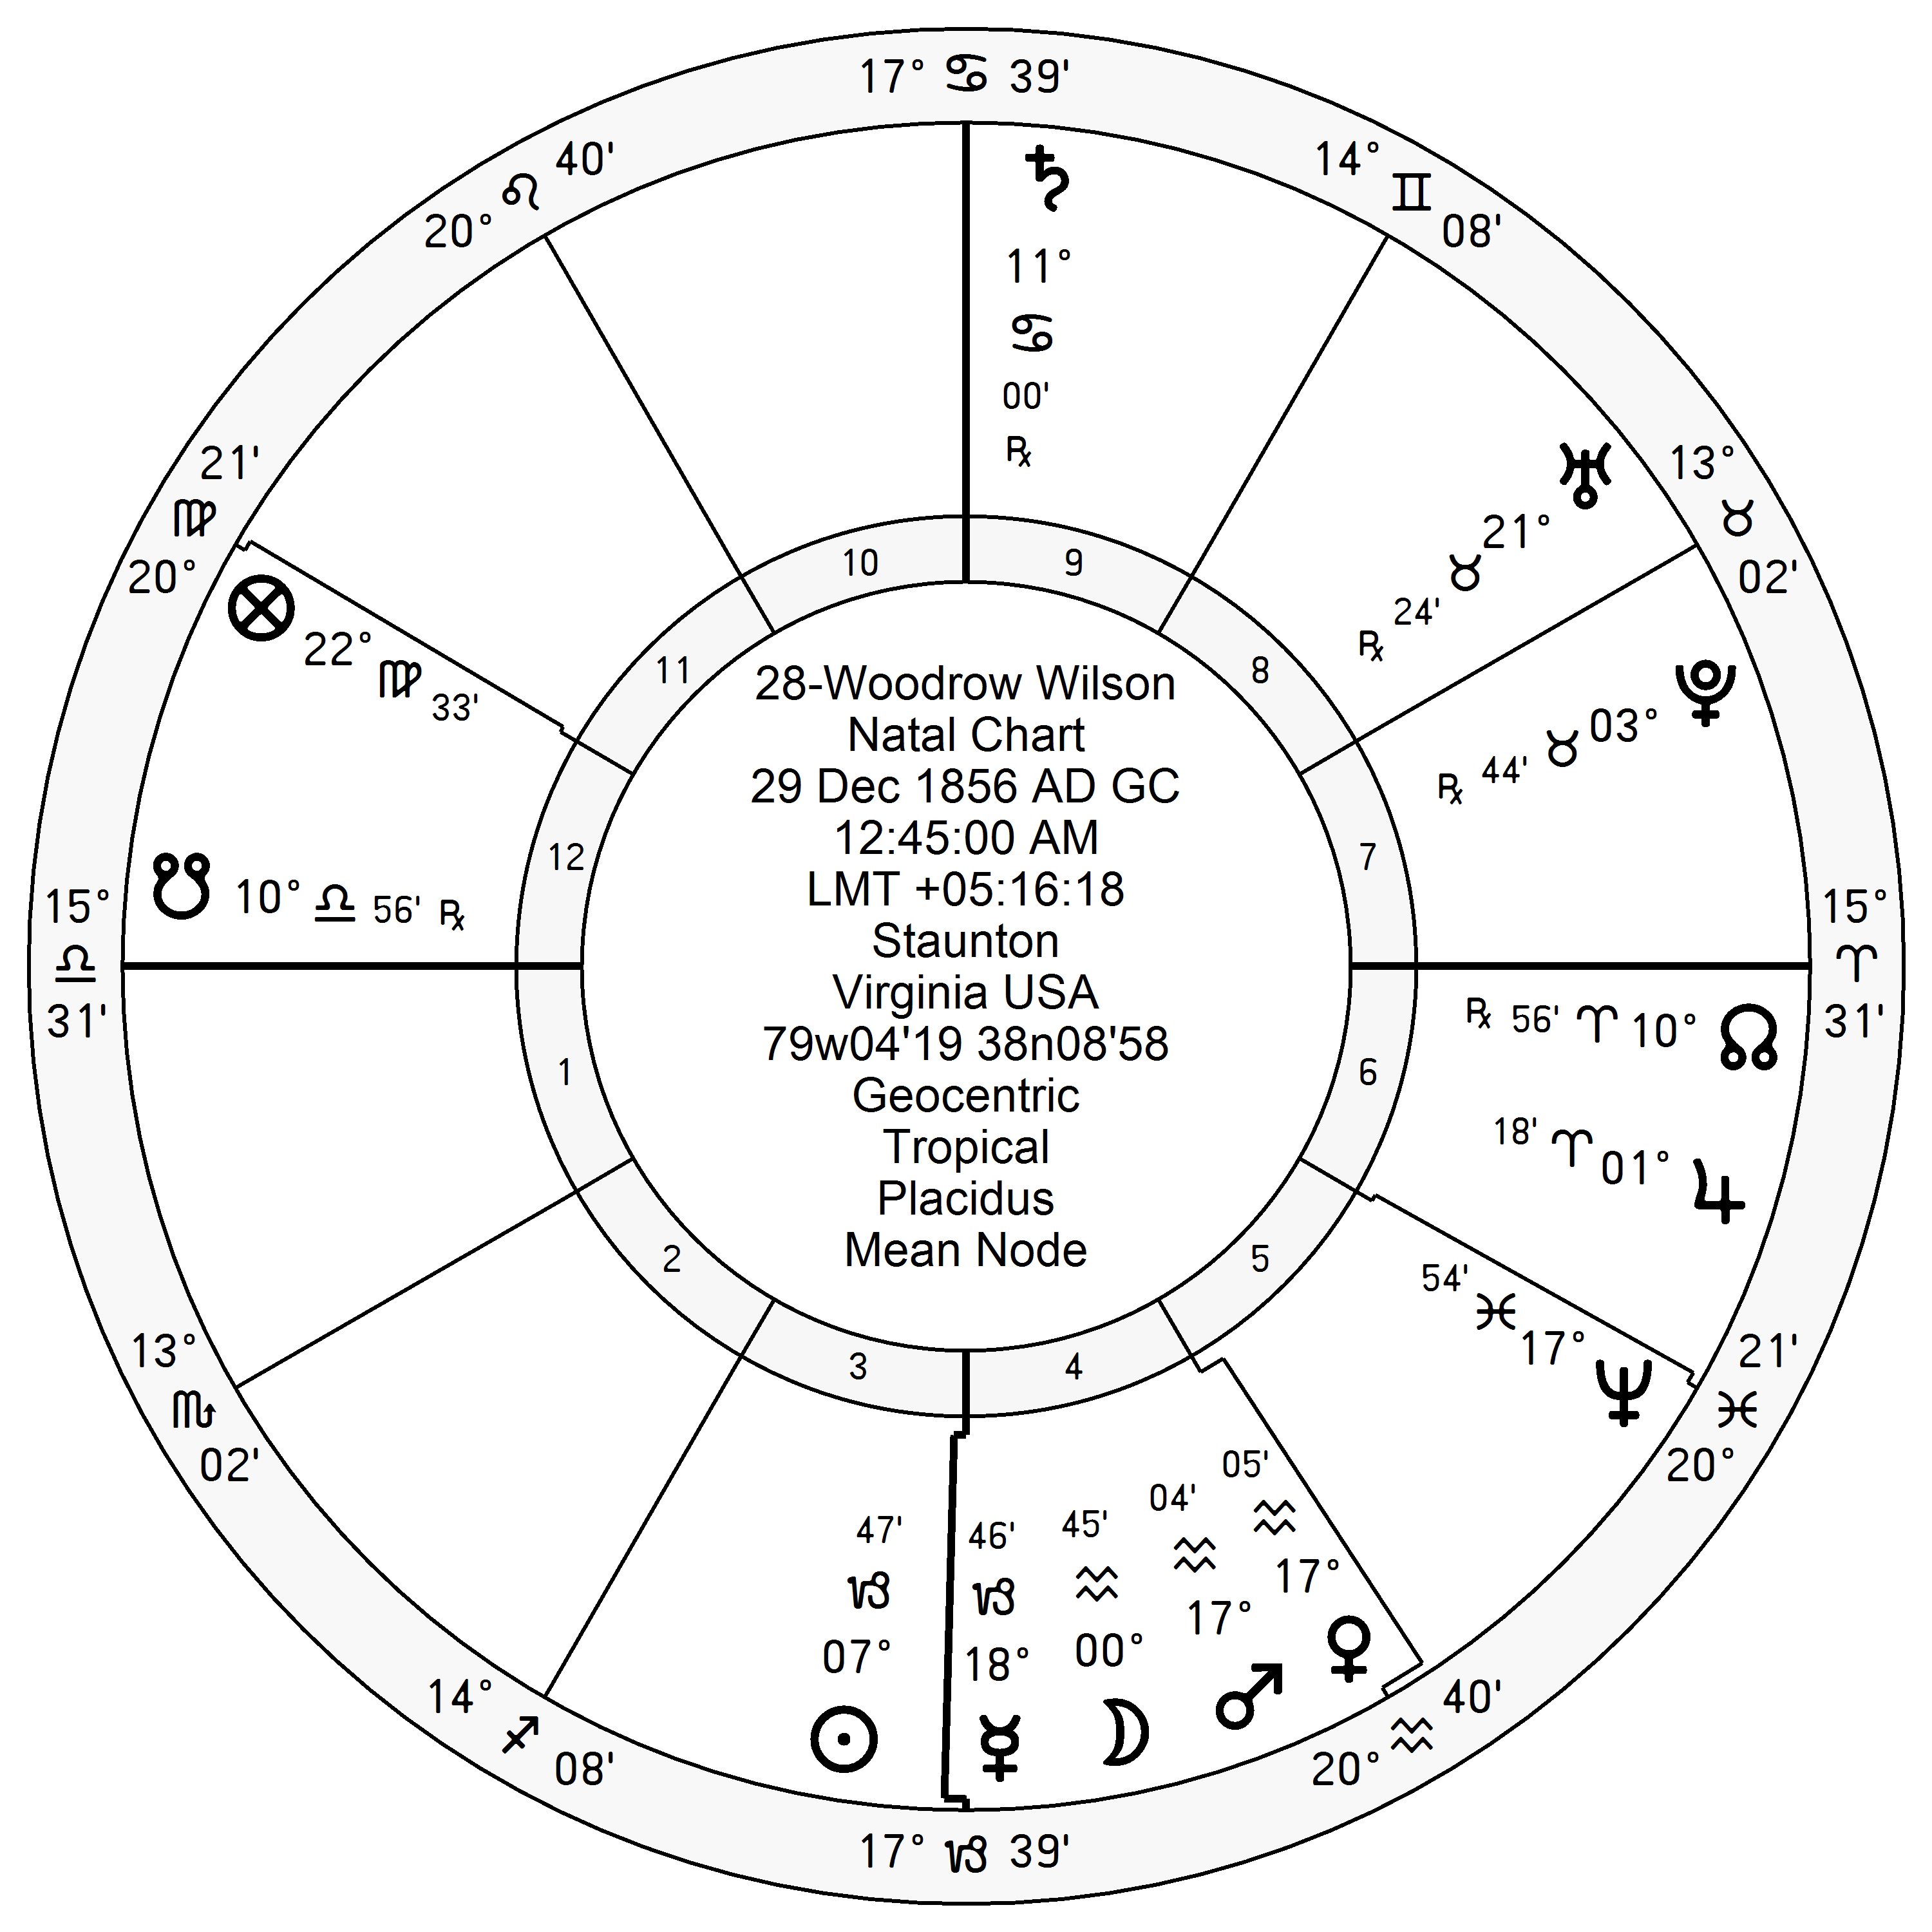
\includegraphics[width=0.9\textwidth]{charts/Wilson.png}}
\fontsize{7pt}{8pt}\selectfont

\Mercury\, \Opposition\, N10; \Trine\, P1, \Square\, N1 \\
\Moon\, \Trine\, N1


\column{0.48\textwidth}
\vspace{-1em}
{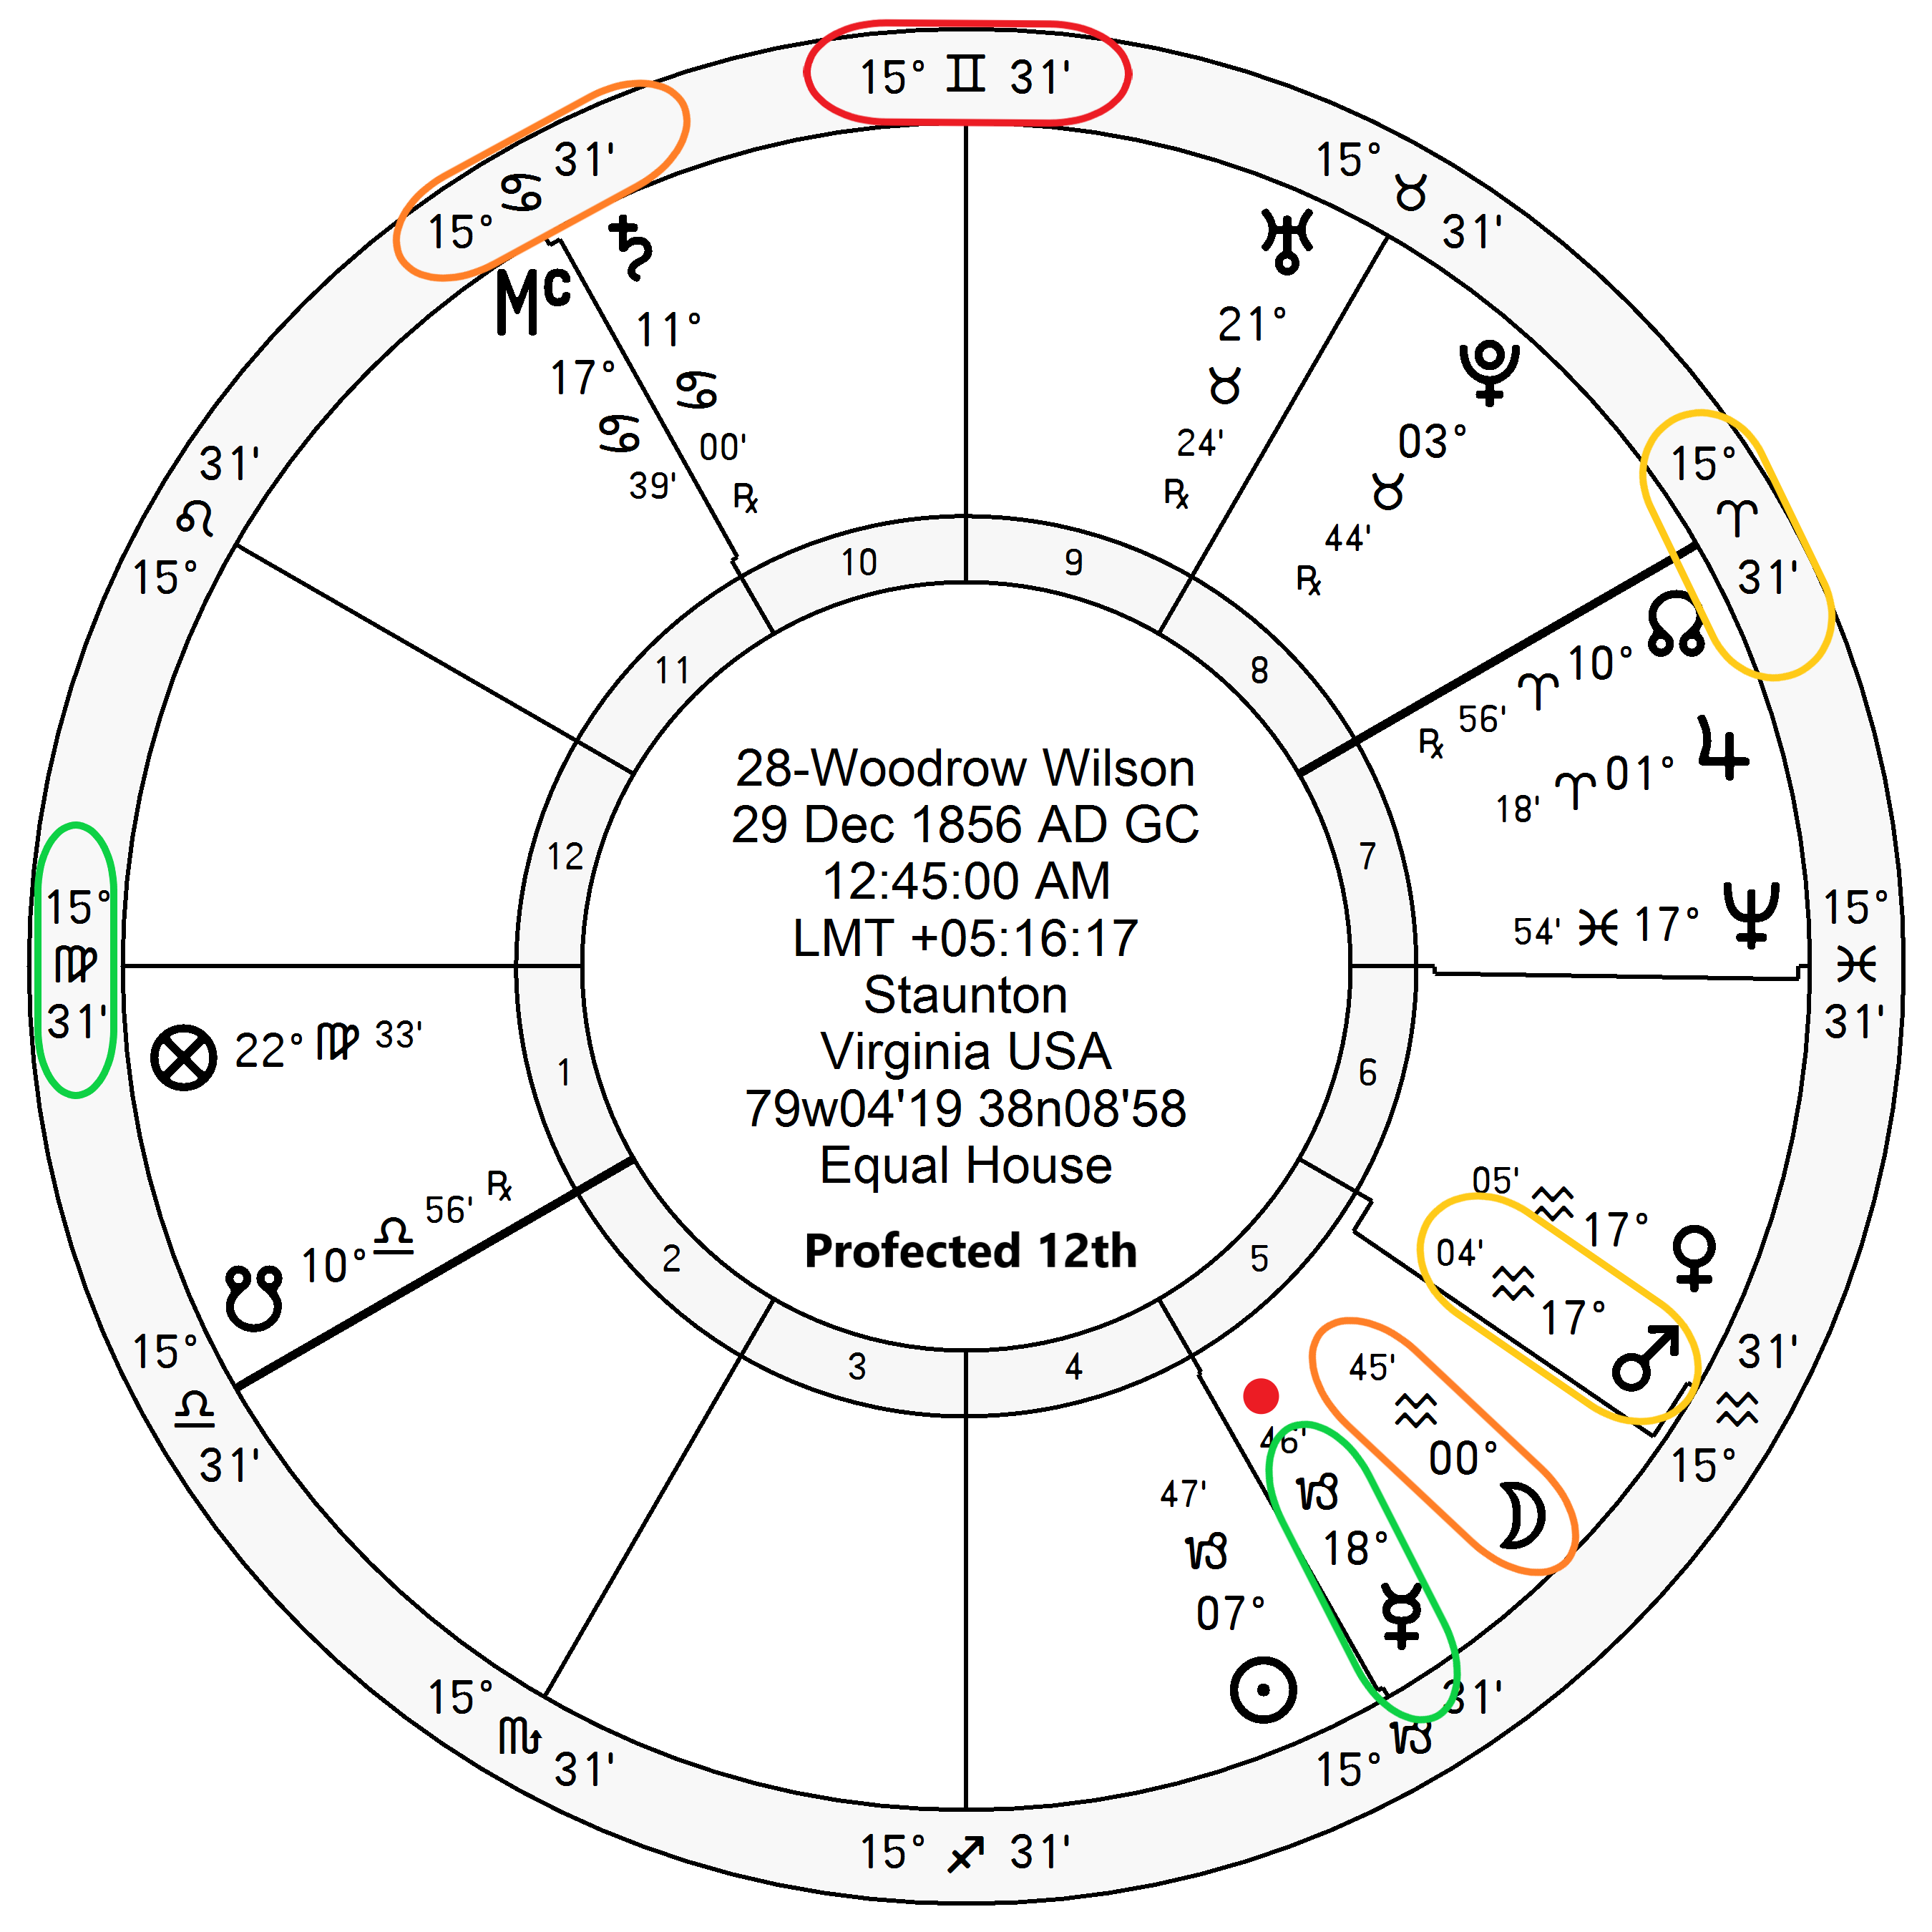
\includegraphics[width=0.9\textwidth]{charts/Wilson-Prof-12th.png}}
\textbf{\dgreen P1}=N12
	$\Rightarrow$ \Mercury\, $\Rightarrow$ \textbf{\dgreen P5/N4} \\
\textbf{\red P10}=N9
	$\Rightarrow$  \Mercury\, $\Rightarrow$ \textbf{\dgreen P5/N4} \\
PE=P11/\textbf{\red N10}
	$\Rightarrow$  \Moon\, $\Rightarrow$   \textbf{\dgreen P5/N4}

\end{columns}
\end{frame}

% Roosevelt
\begin{frame}[t]{Election November 7, 1916: Charles Evans Hughes}
\small
\begin{columns}[T, onlytextwidth]
\column{0.48\textwidth}
\vspace{-1em}
{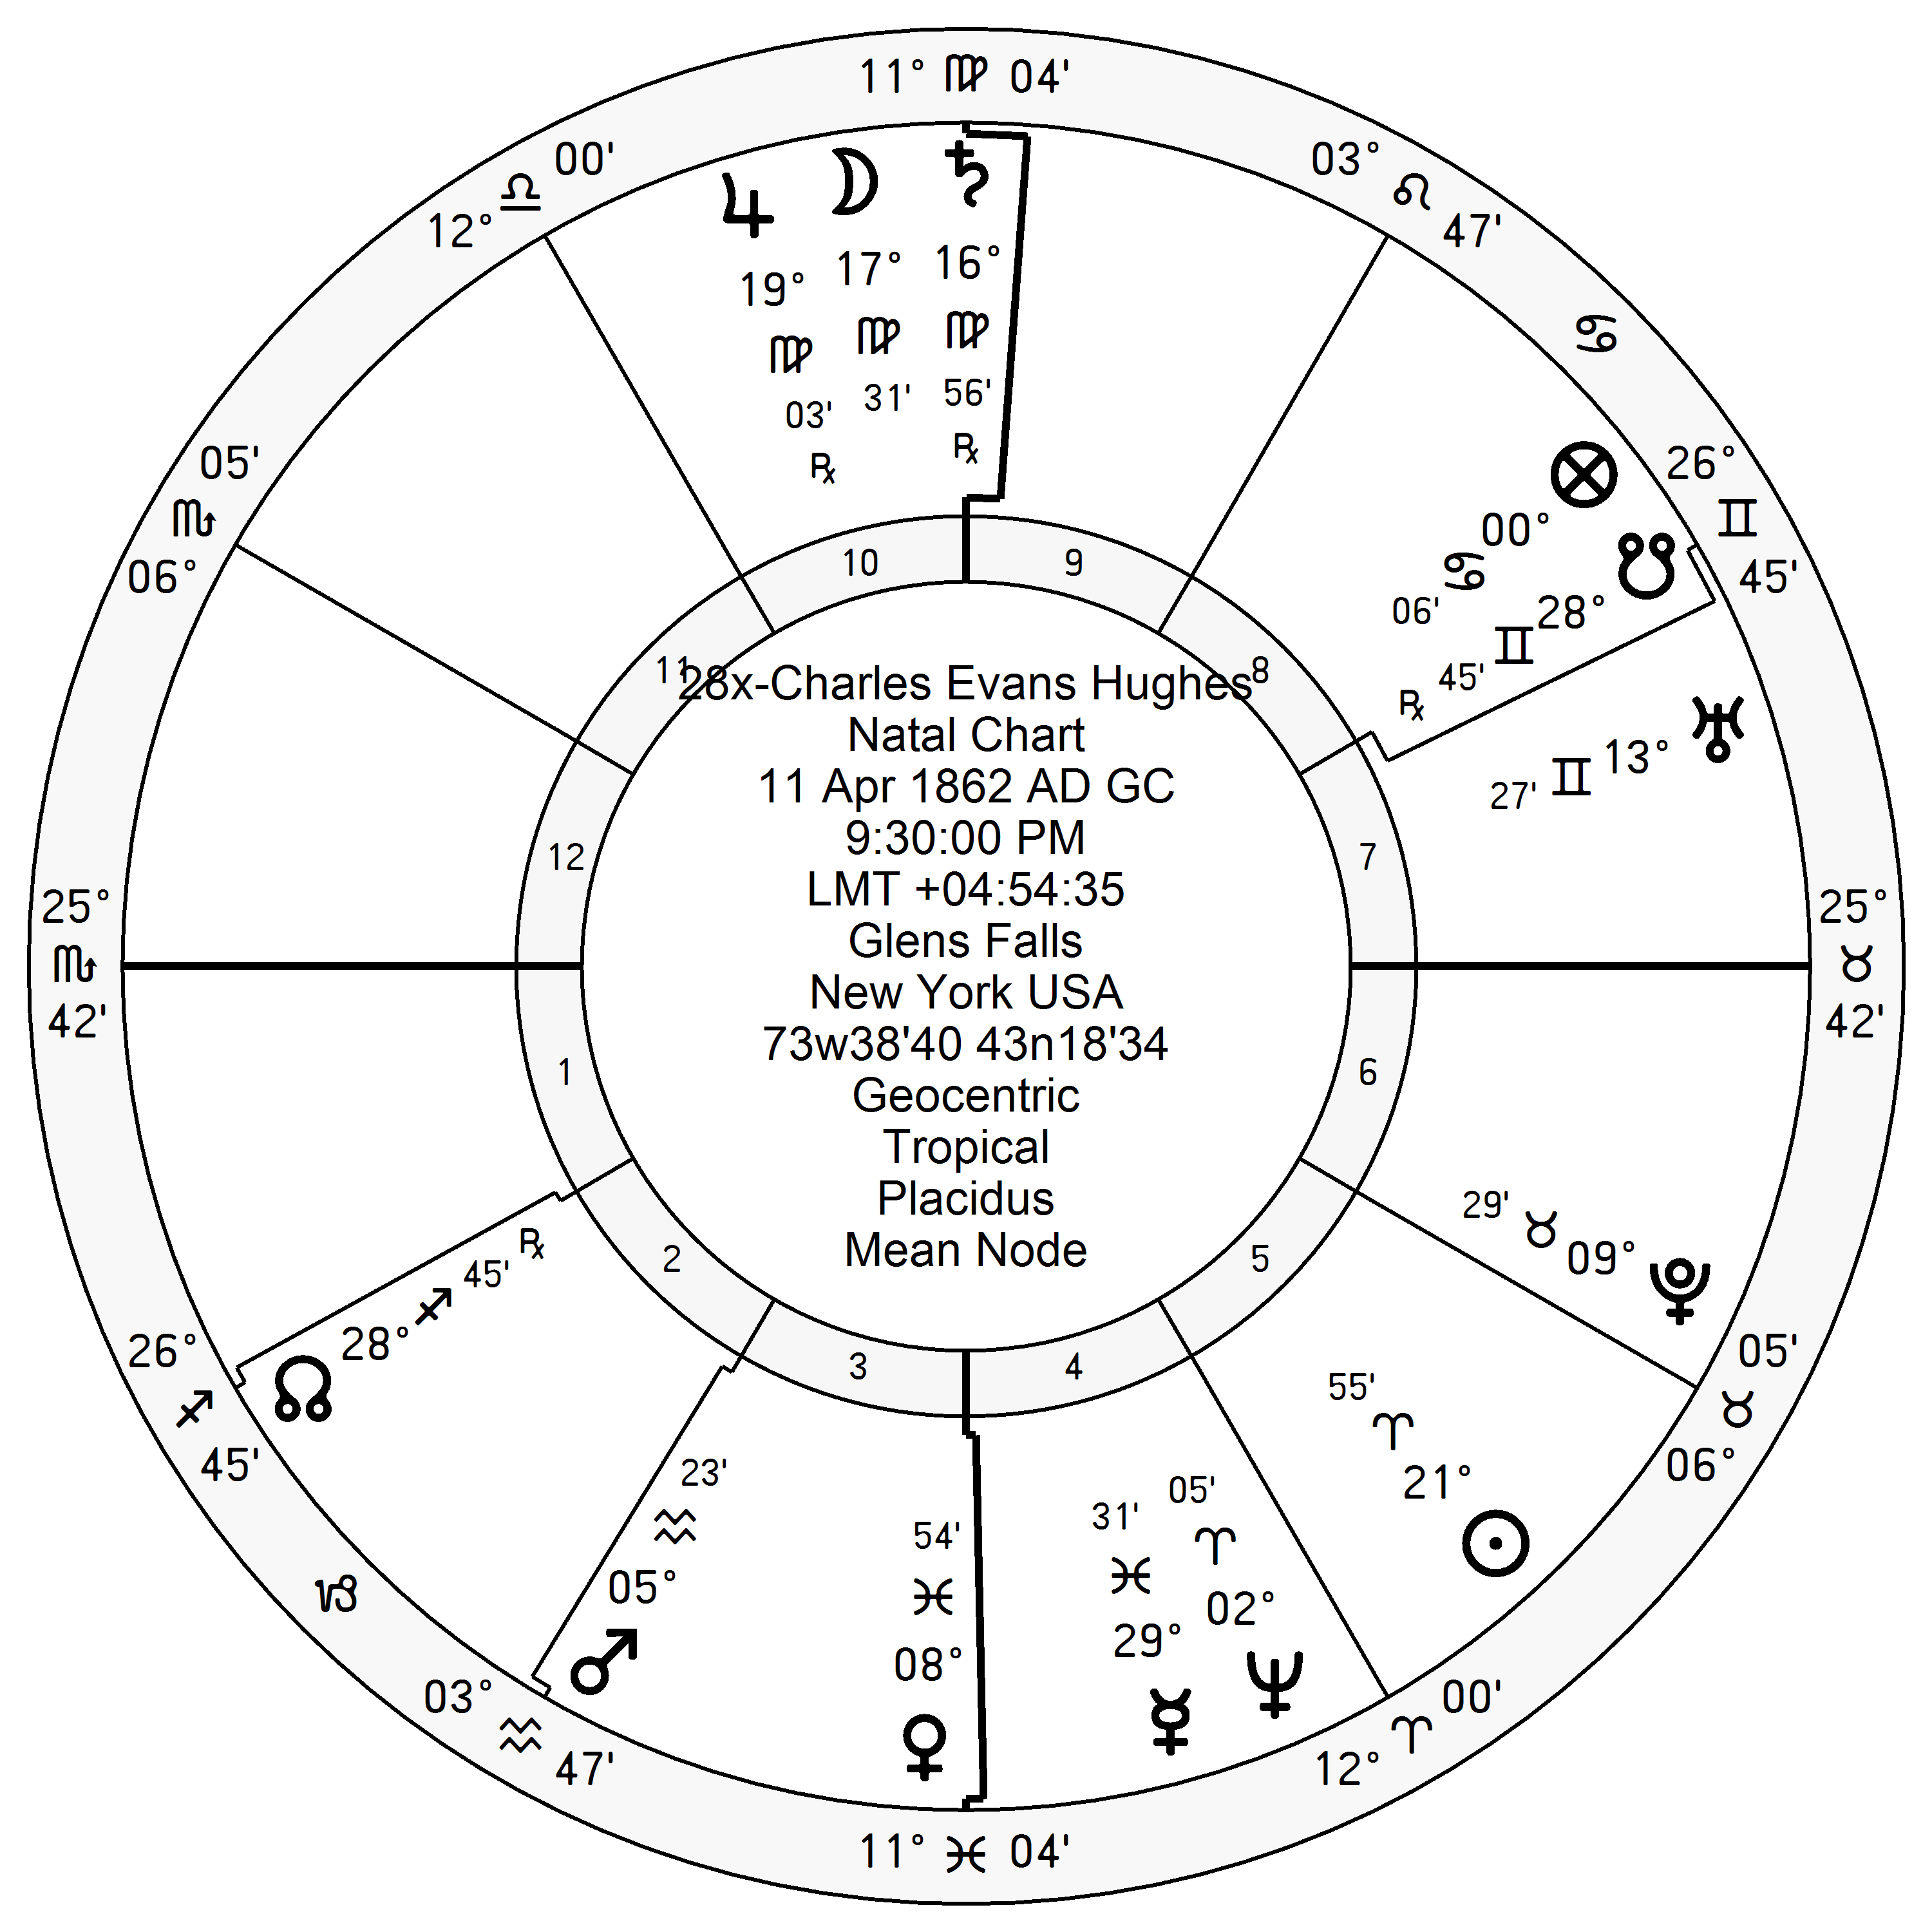
\includegraphics[width=0.9\textwidth]{charts/Hughes.png}}
\fontsize{8pt}{9pt}\selectfont

\Venus\, in P10, \Square\, P1, N1 \\
\Saturn\, \Opposition\, \Venus\, in P10, \Square\, P1; in N10 \\
\Mars\, \Trine\, P1, \Sextile\, N1 \\
\vspace{1em}
\Saturn\, in bad state (retro, disposited by \Mercury\, in Fall; \Square\, \Uranus) denies what the 10th promises?

\column{0.48\textwidth}
\vspace{-1em}
{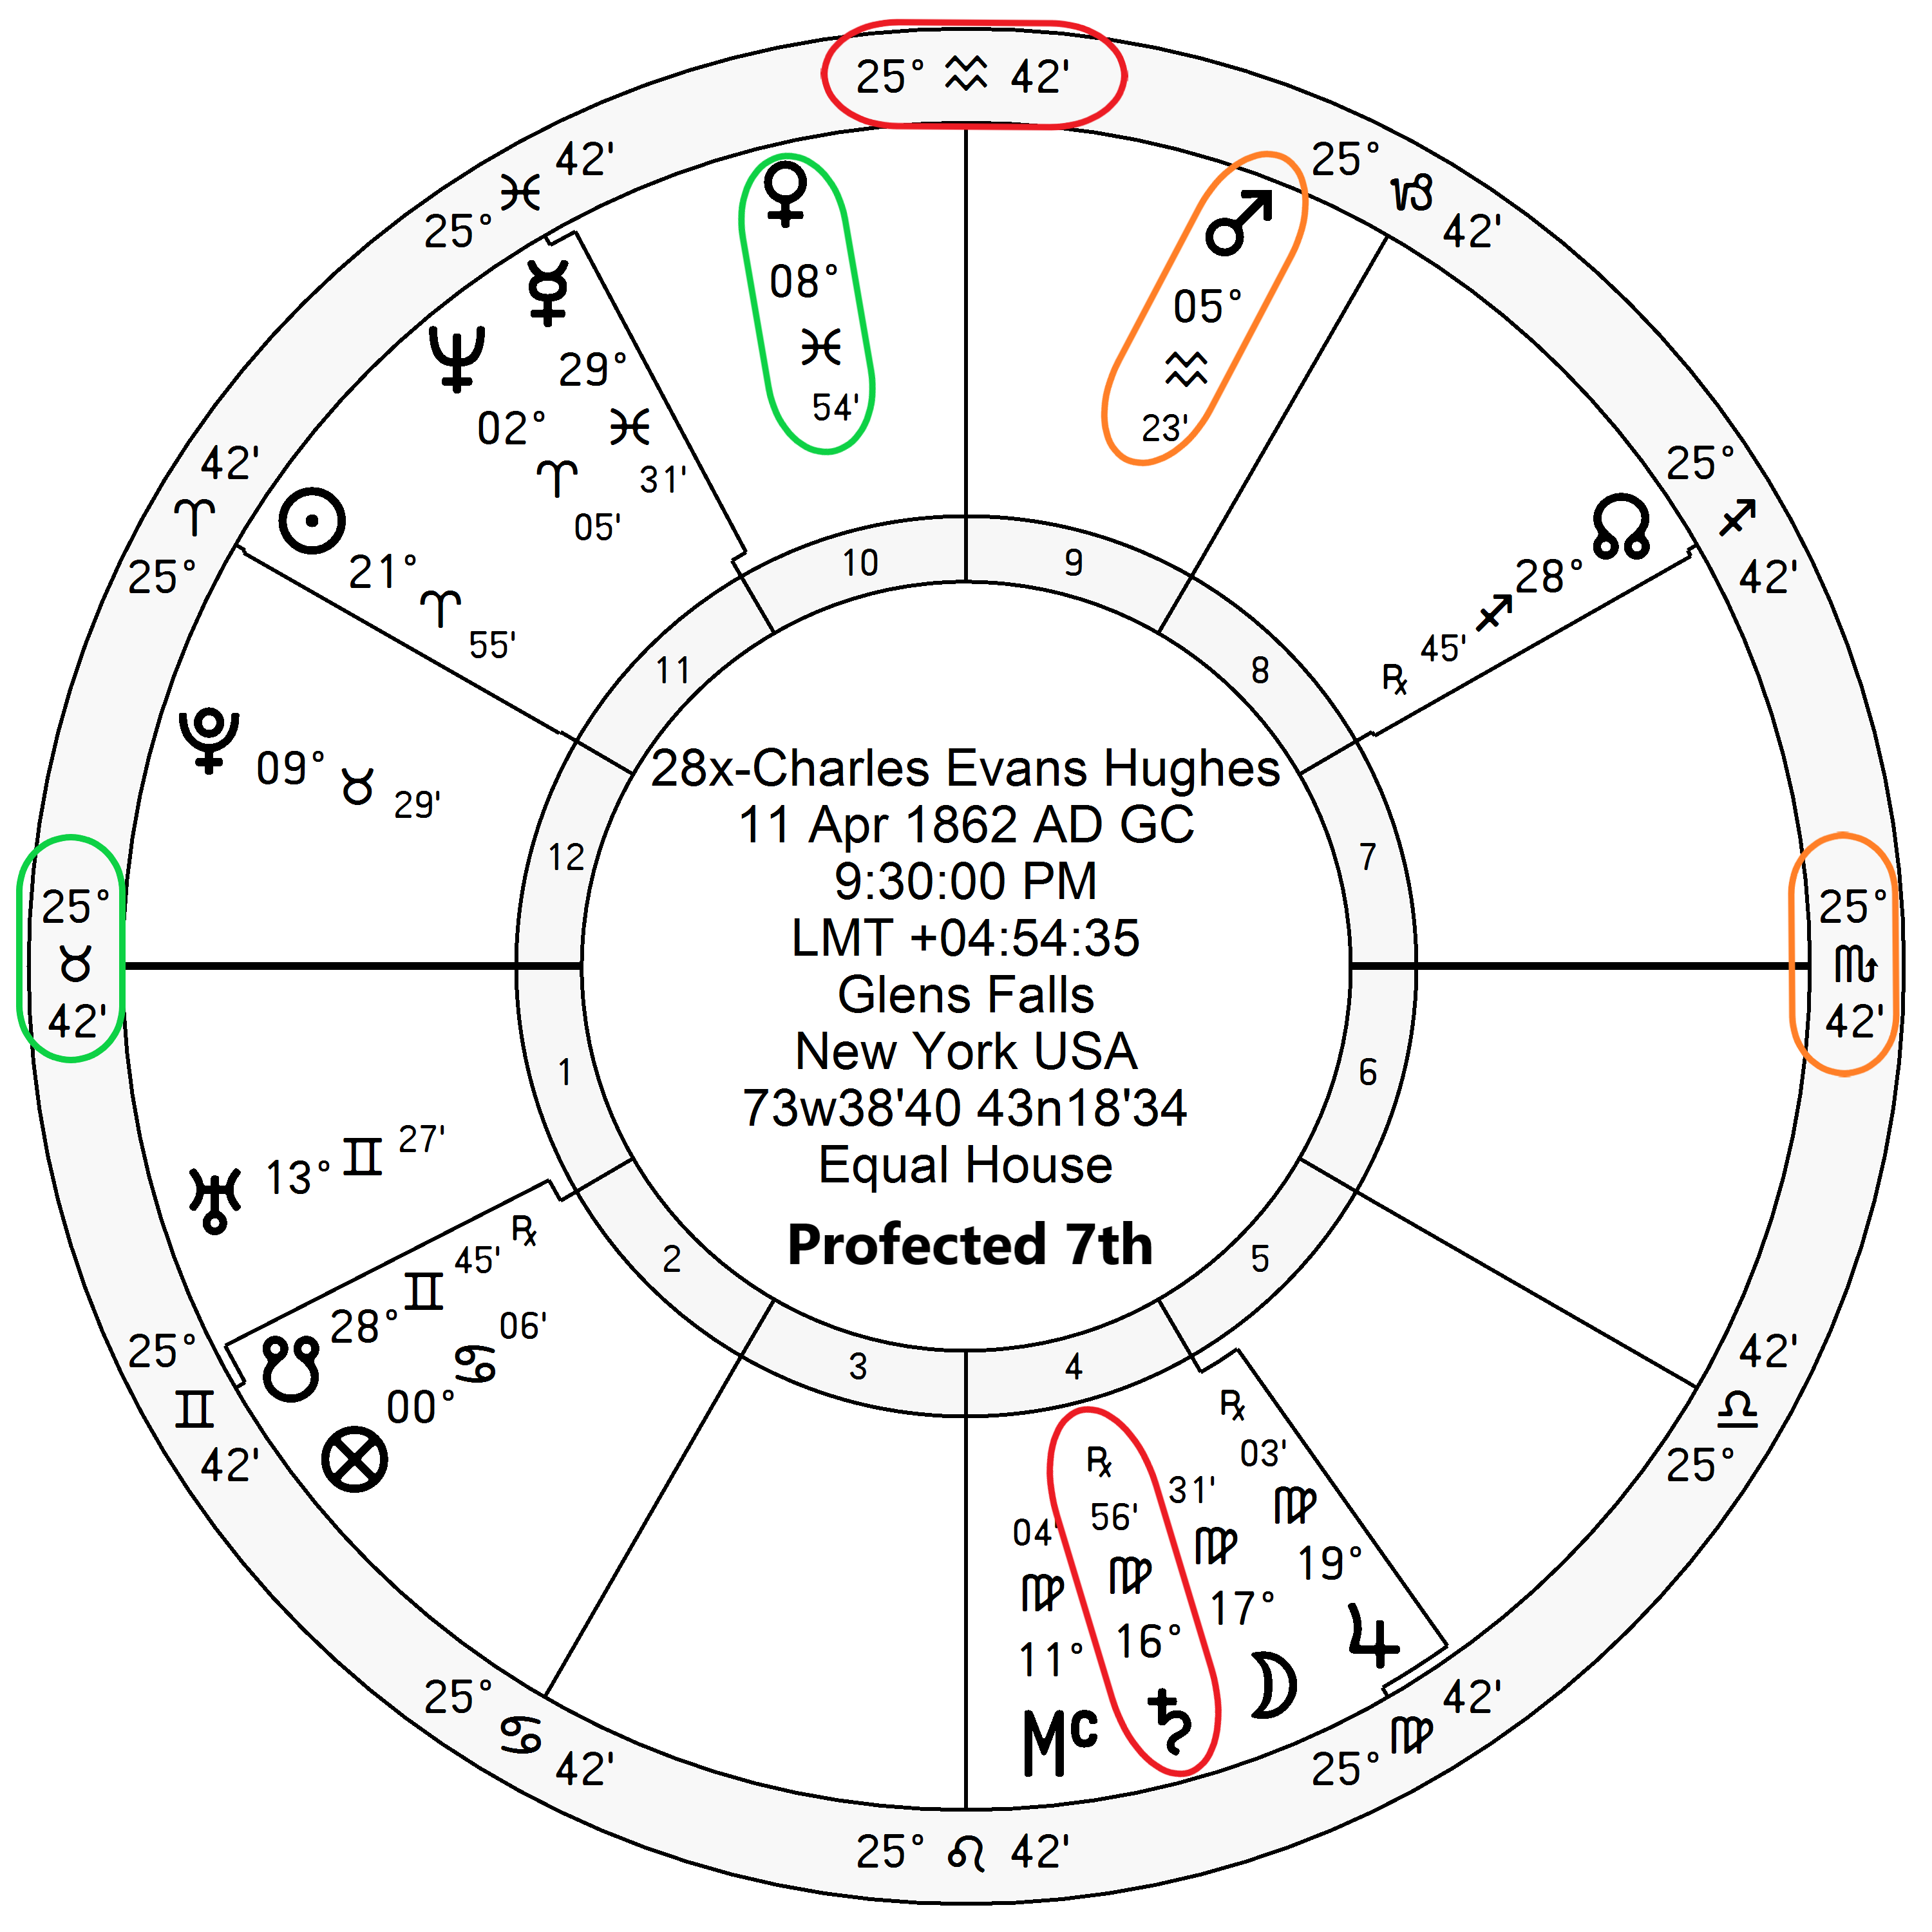
\includegraphics[width=0.9\textwidth]{charts/Hughes-Prof-7th.png}}
\textbf{\dgreen P1=N7} 
	$\Rightarrow$ \Venus\, $\Rightarrow$ \textbf{\red P10/N3}\\
\textbf{\red P10=N3}
	$\Rightarrow$ \Saturn\,\Retrograde $\Rightarrow$ P4/\textbf{\red N10}\\
PE=\textbf{\dgreen P7/}N12
	$\Rightarrow$ \Mars\, $\Rightarrow$ P9/\textbf{\red N3}


\end{columns}
\end{frame}

%\subsection{Election November 3, 1936: *Roosevelt vs Landon}
\begin{frame}[t]{Election November 3, 1936: *Franklin Roosevelt}
\small

\begin{columns}[T, onlytextwidth]
\column{0.48\textwidth}
\vspace{-1em}
{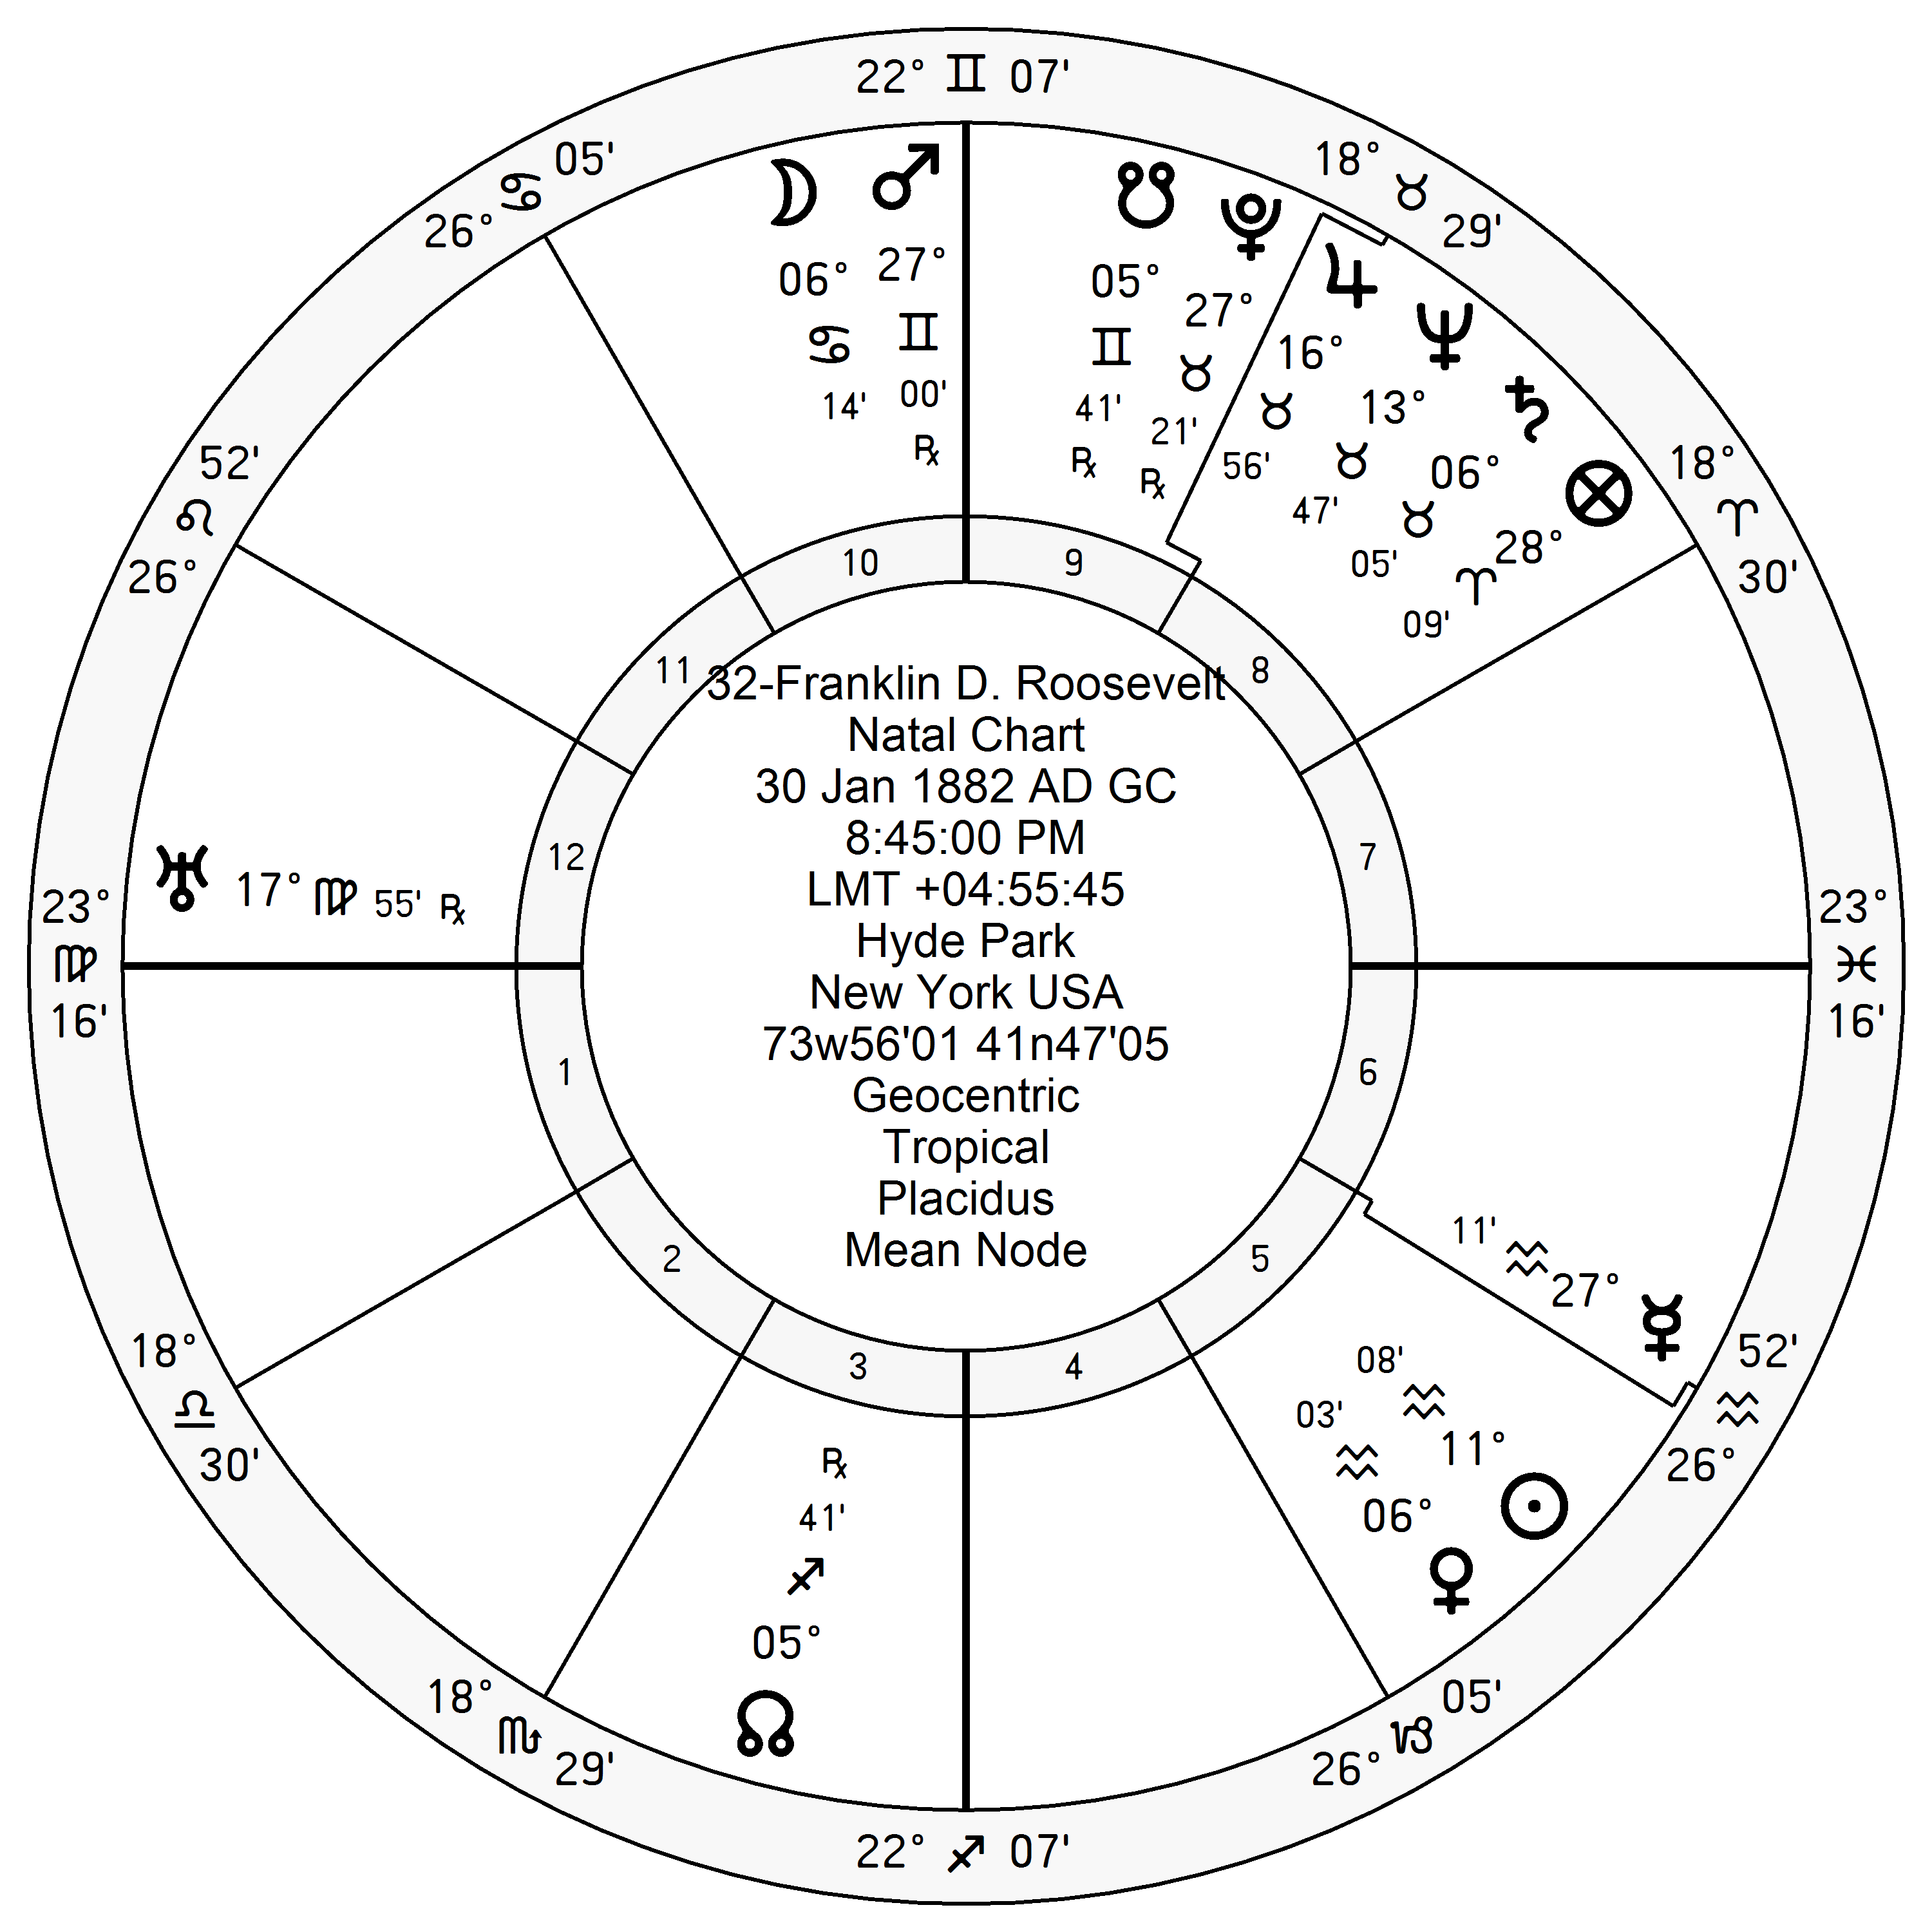
\includegraphics[width=0.9\textwidth]{charts/FDR.png}}
\fontsize{7pt}{8pt}\selectfont

\Jupiter\, \Trine\, P10, \Sextile\, N10, P1; in a mitigated \Quincunx\, (\Opposition) with N1 which appears to have been enough for the win as his opponent has only one hard aspect involving a burnt \Mercury.

\column{0.48\textwidth}
\vspace{-1em}
{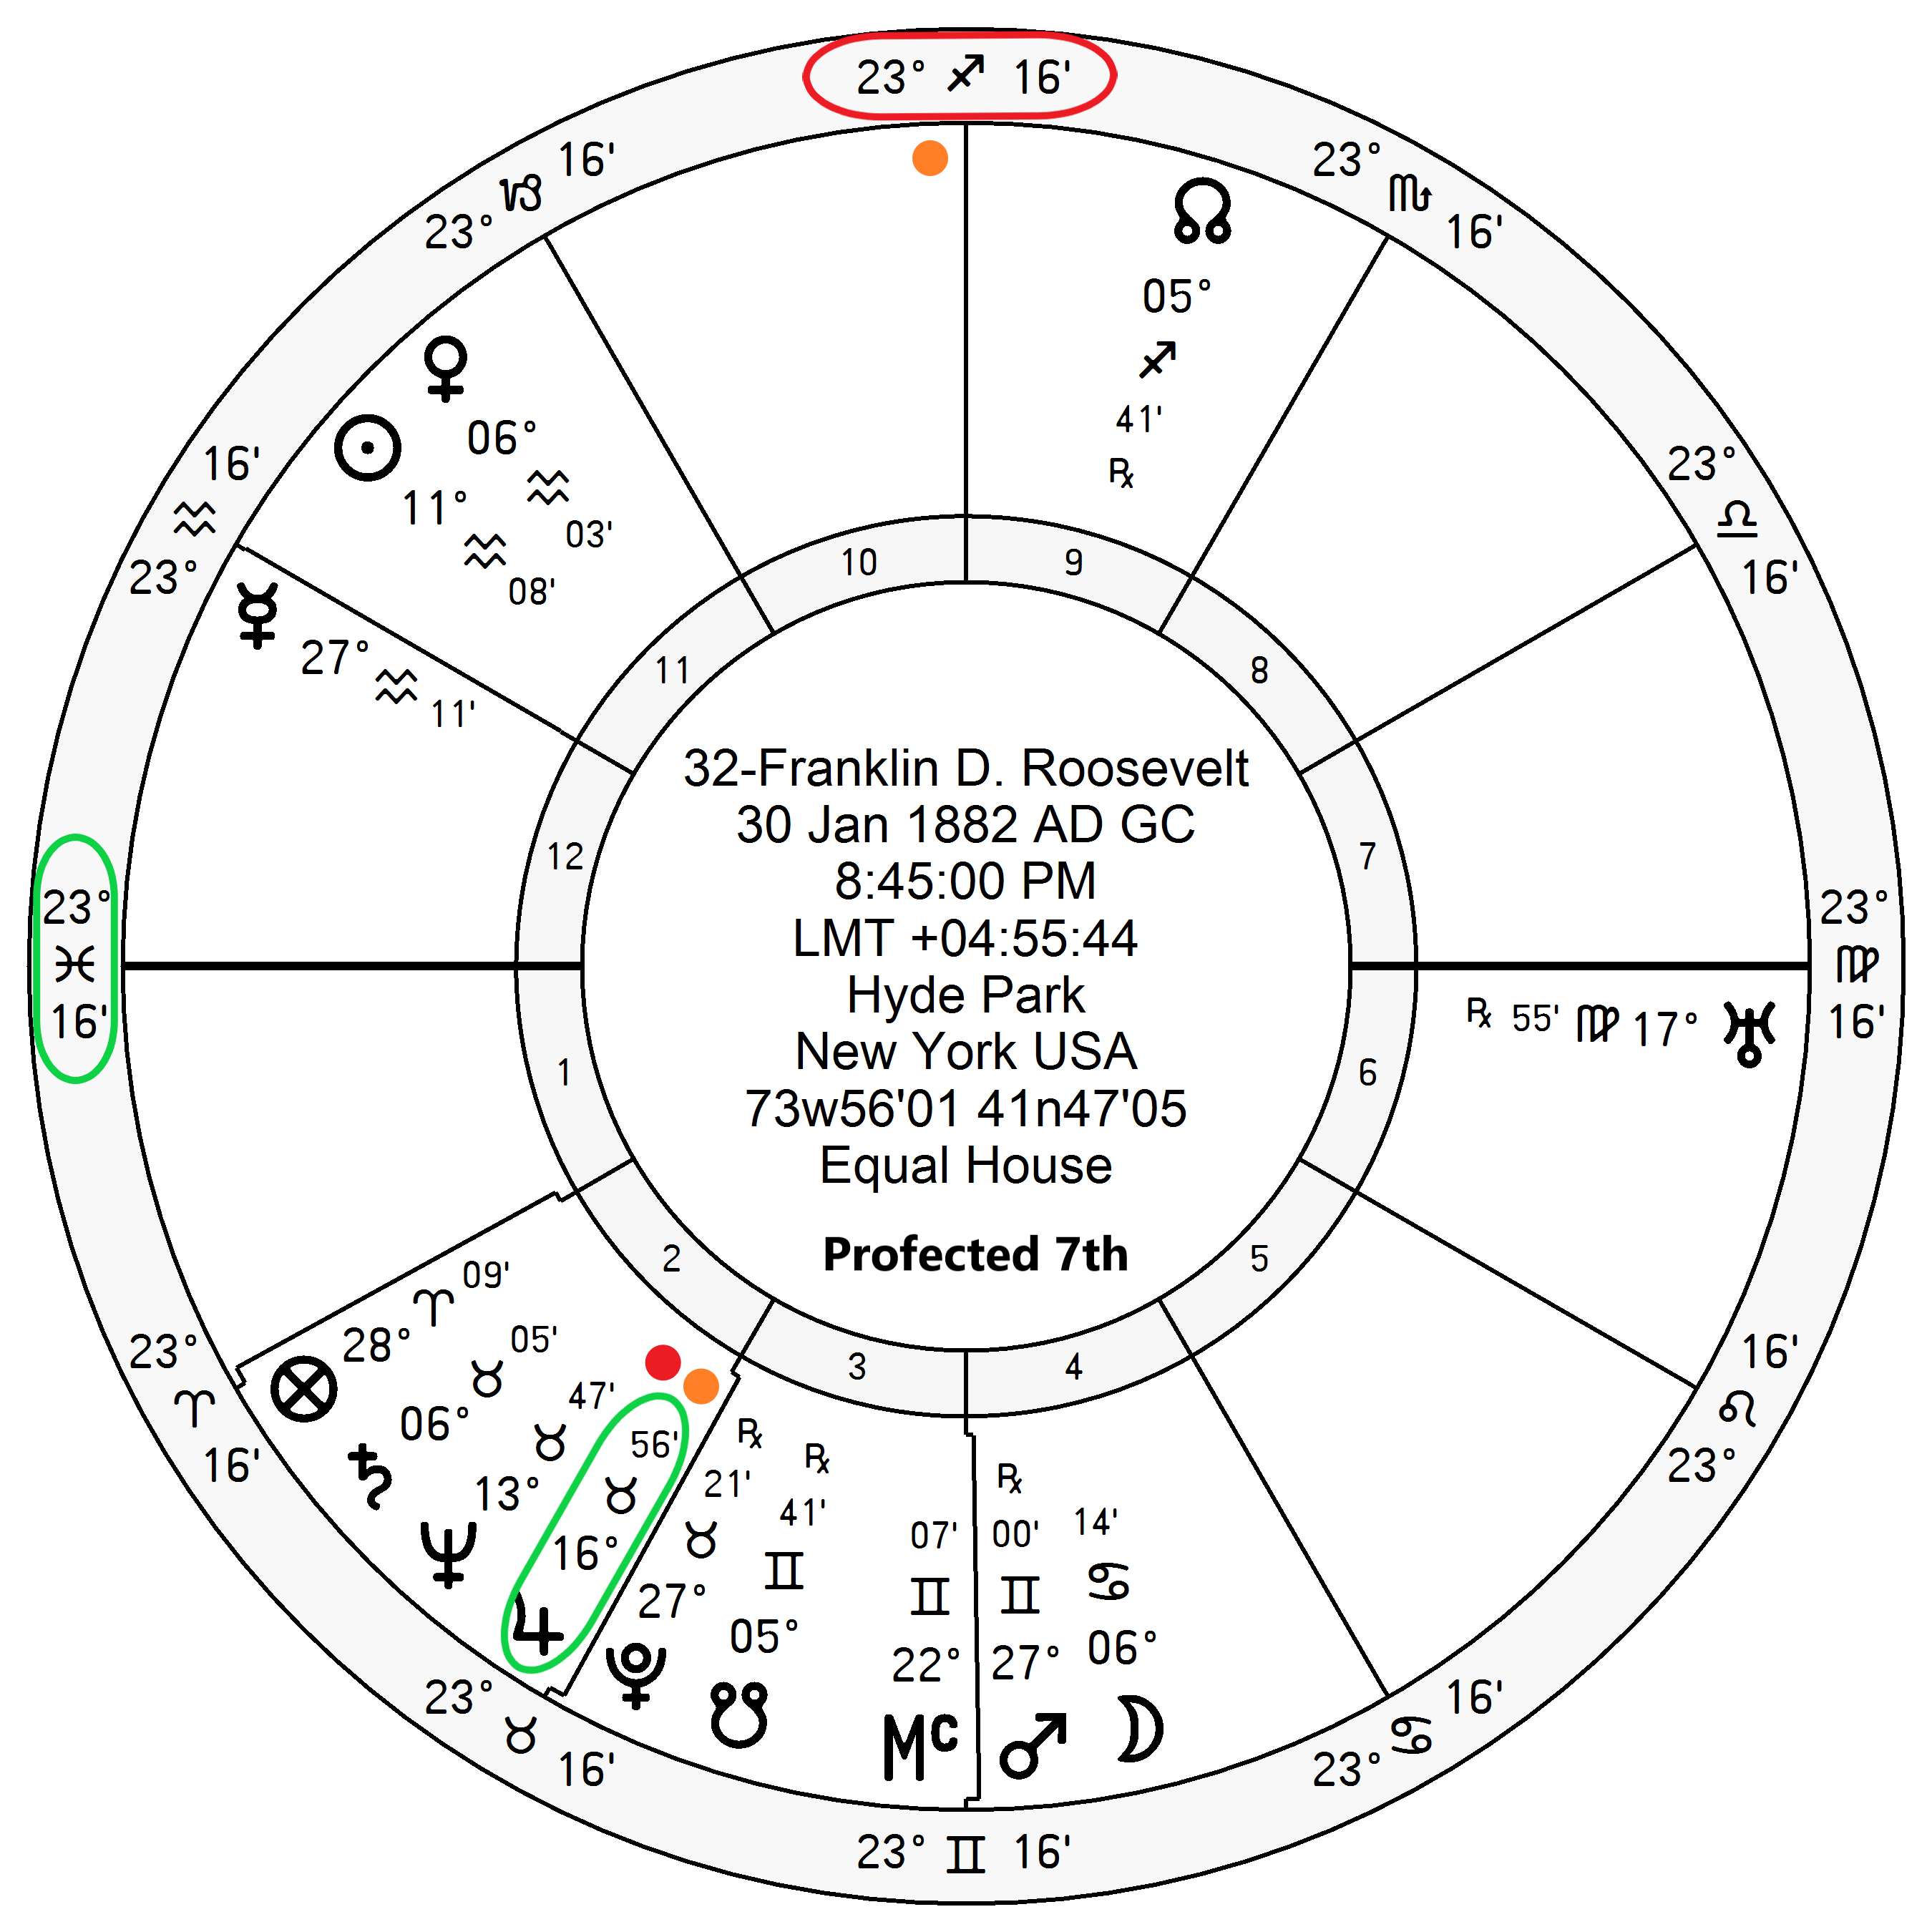
\includegraphics[width=0.9\textwidth]{charts/FDR-Prof-7th.png}}

\textbf{\dgreen P1}=N7
	$\Rightarrow$ \Jupiter\, $\Rightarrow$ \textbf{\dgreen P2/N8} \\
\textbf{\red P10=N4}
	$\Rightarrow$  \Jupiter\, $\Rightarrow$ \textbf{\dgreen P2/N8} \\
PE=\textbf{\red P10/N4}
	$\Rightarrow$  \Jupiter\, $\Rightarrow$   \textbf{\dgreen P2/N8}


\end{columns}
\end{frame}

% candidate
\begin{frame}[t]{Election November 3, 1936: Alf Landon}
\small
\begin{columns}[T, onlytextwidth]
\column{0.48\textwidth}
\vspace{-1em}
{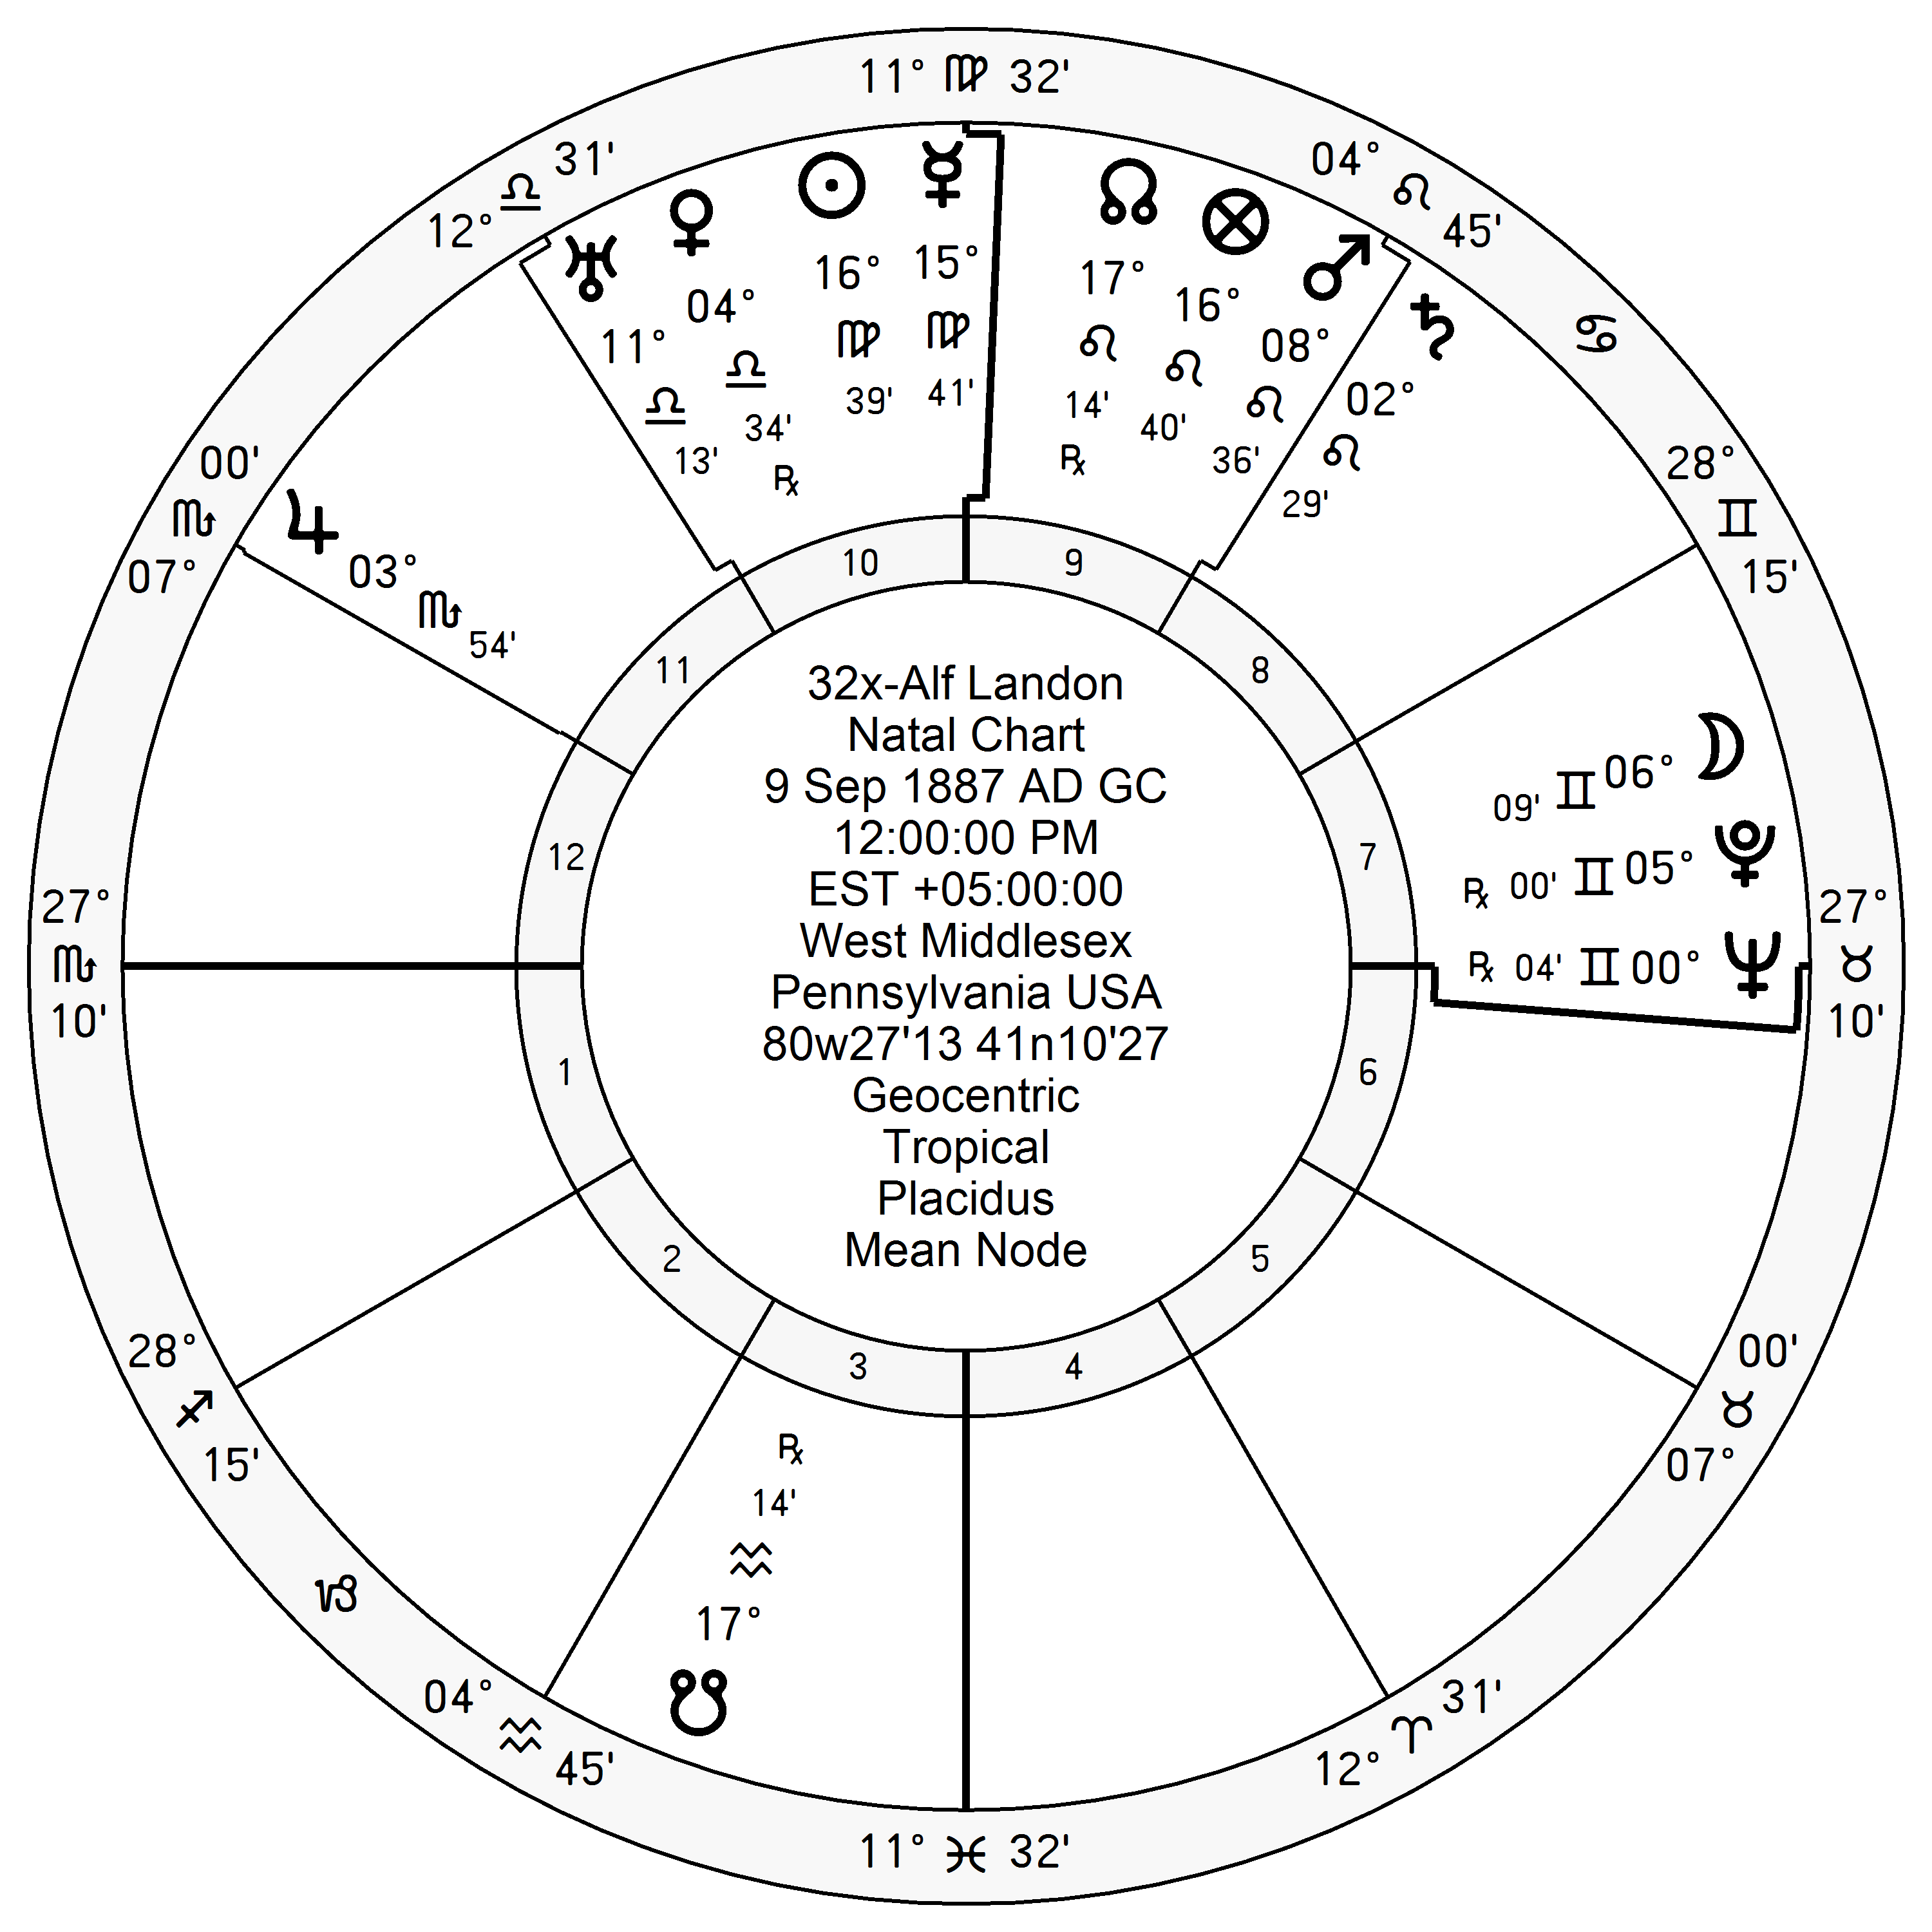
\includegraphics[width=0.9\textwidth]{charts/Landon.png}}
\fontsize{8pt}{9pt}\selectfont

\Jupiter\, \Sextile\, P1 \\
\Mercury\, (burnt) \Trine\, P1 in N10; \Square\, N1 \\
\Saturn\, \Sextile\, P10


\column{0.48\textwidth}
\vspace{-1em}
{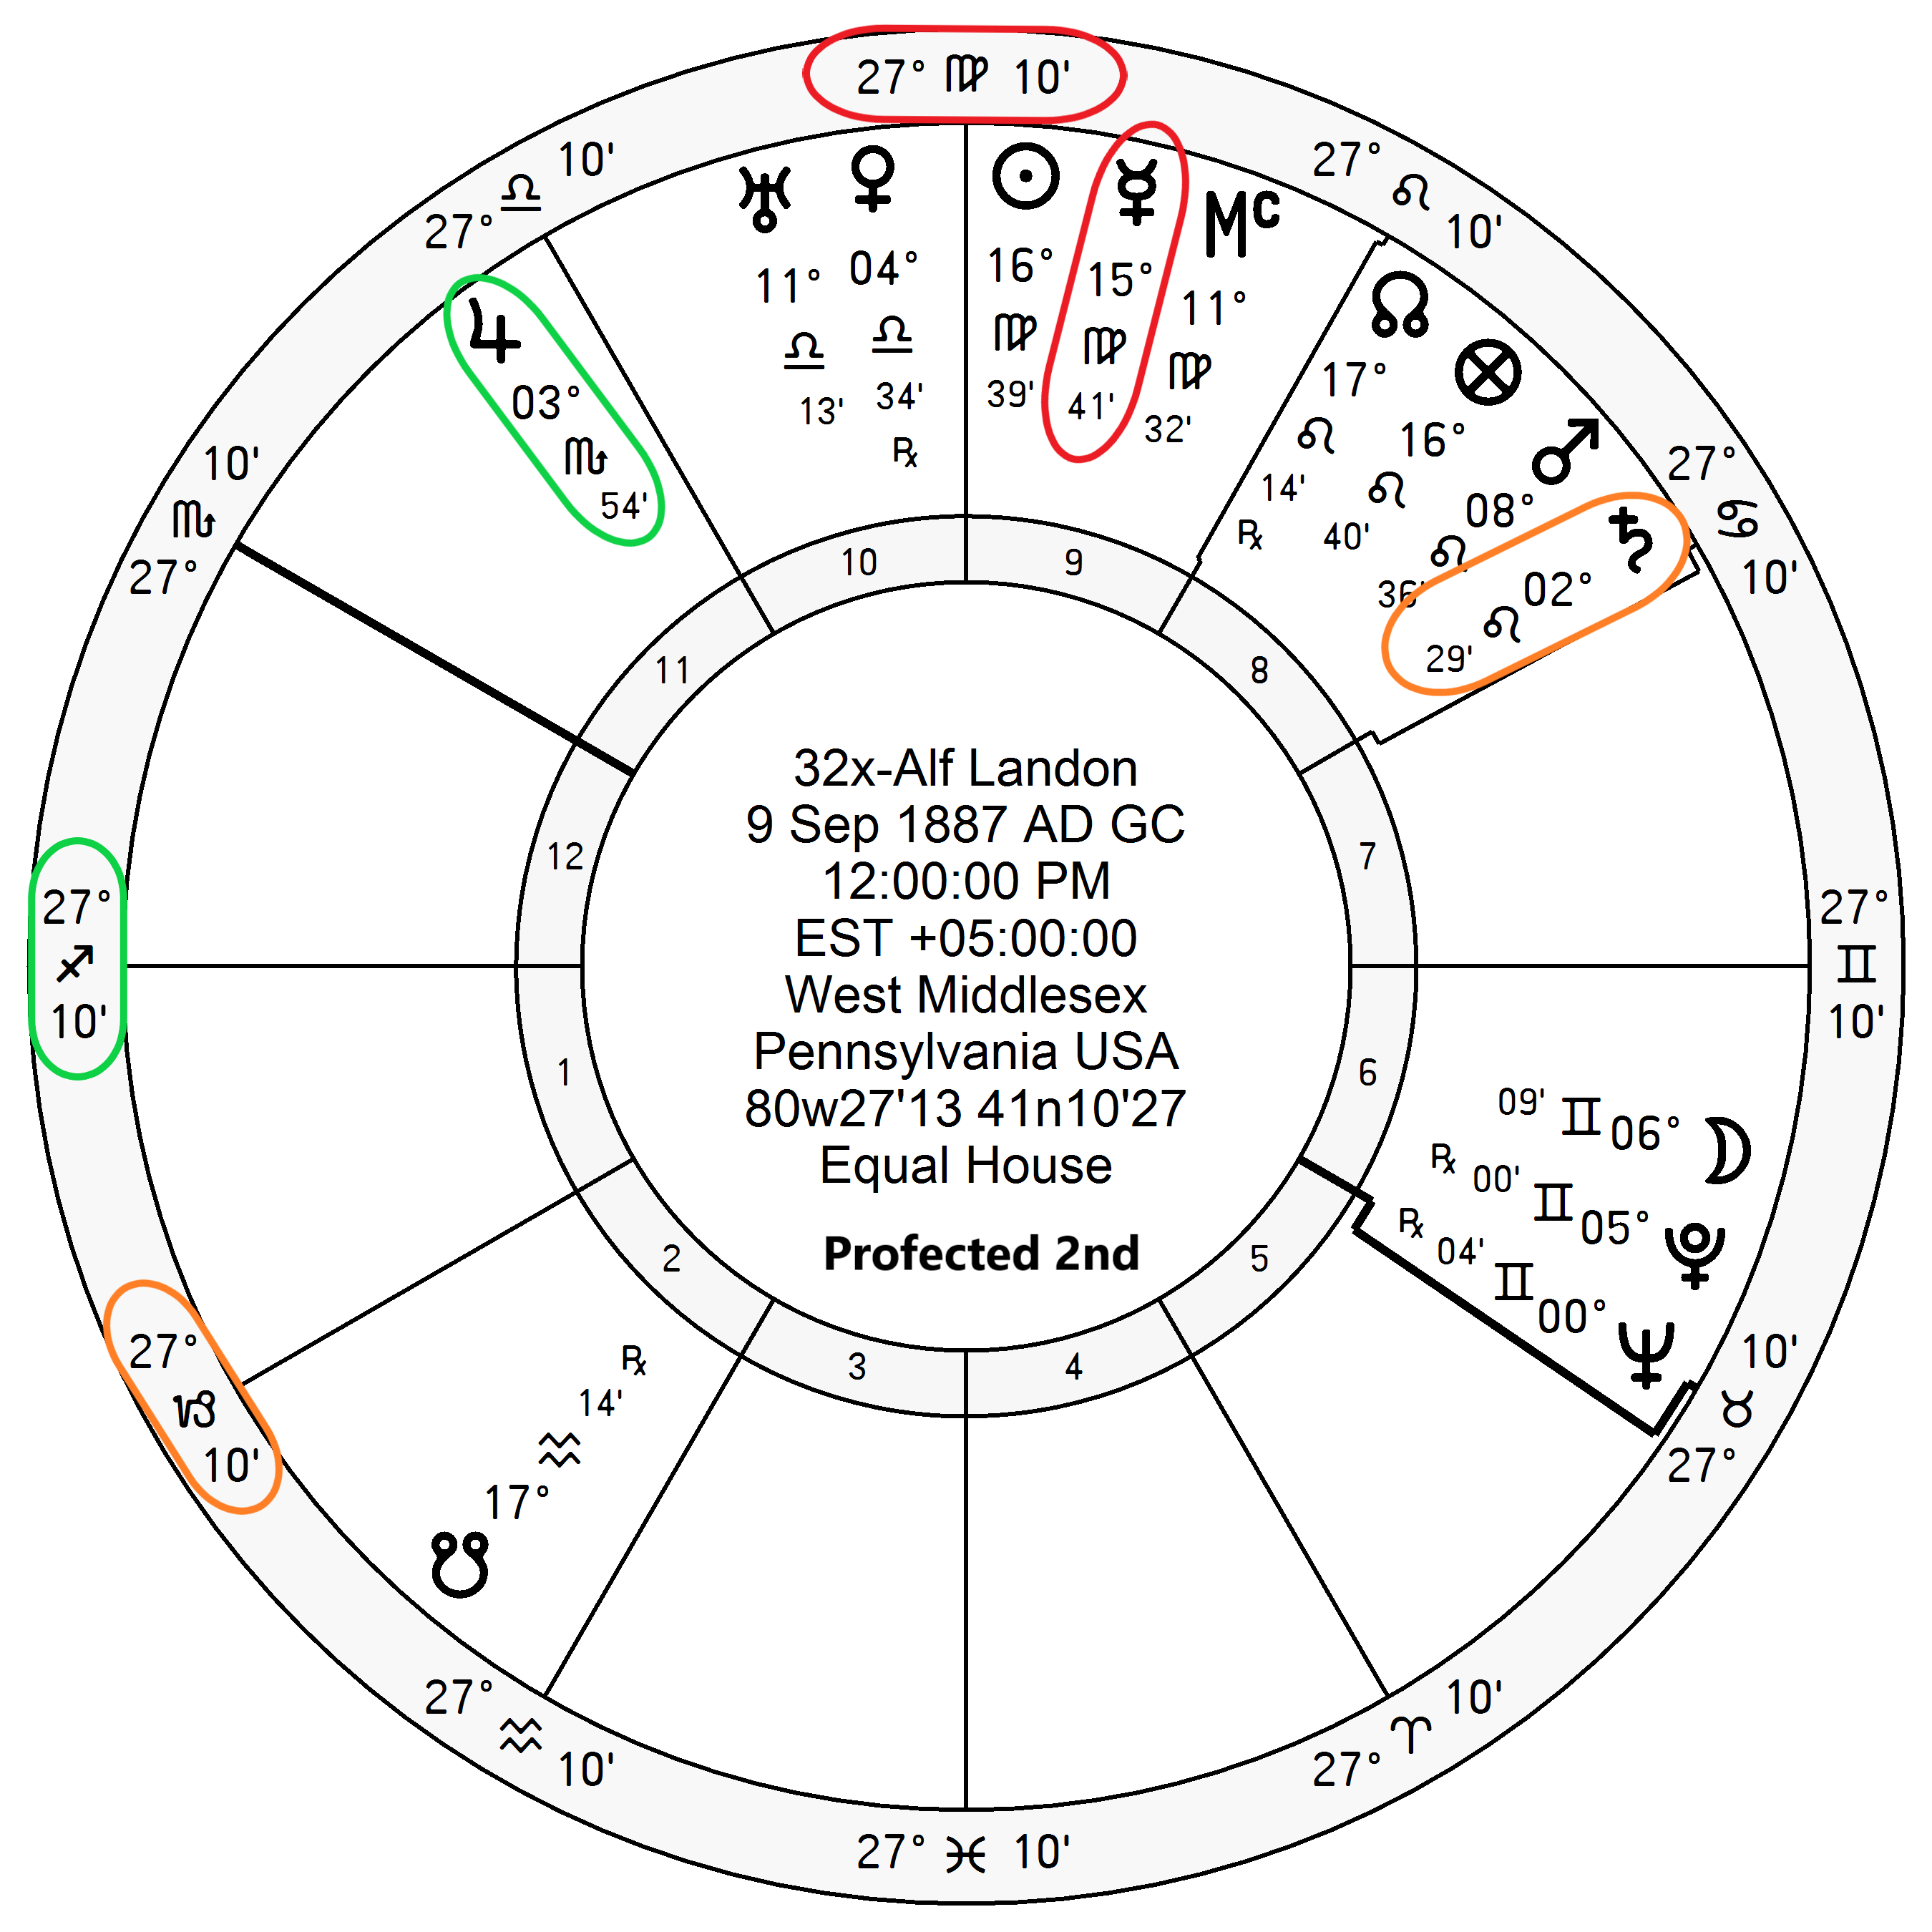
\includegraphics[width=0.9\textwidth]{charts/Landon-Prof-2nd.png}}

\textbf{\dgreen P1=N2} 
	$\Rightarrow$ \Jupiter\, $\Rightarrow$ P11/N11\\
\textbf{\red P10=N10}
	$\Rightarrow$ \Mercury\, (combust) $\Rightarrow$ P9/\textbf{\red N10}\\
PE=P2/\textbf{\dgreen N2}
	$\Rightarrow$ \Saturn\, $\Rightarrow$ P8/N8

\end{columns}
\end{frame}

%\subsection{Election November 5, 1940: *Roosevelt vs Wilkie}
\begin{frame}[t]{Election November 5, 1940: *Franklin Roosevelt}
\small

\begin{columns}[T, onlytextwidth]
\column{0.48\textwidth}
\vspace{-1em}
{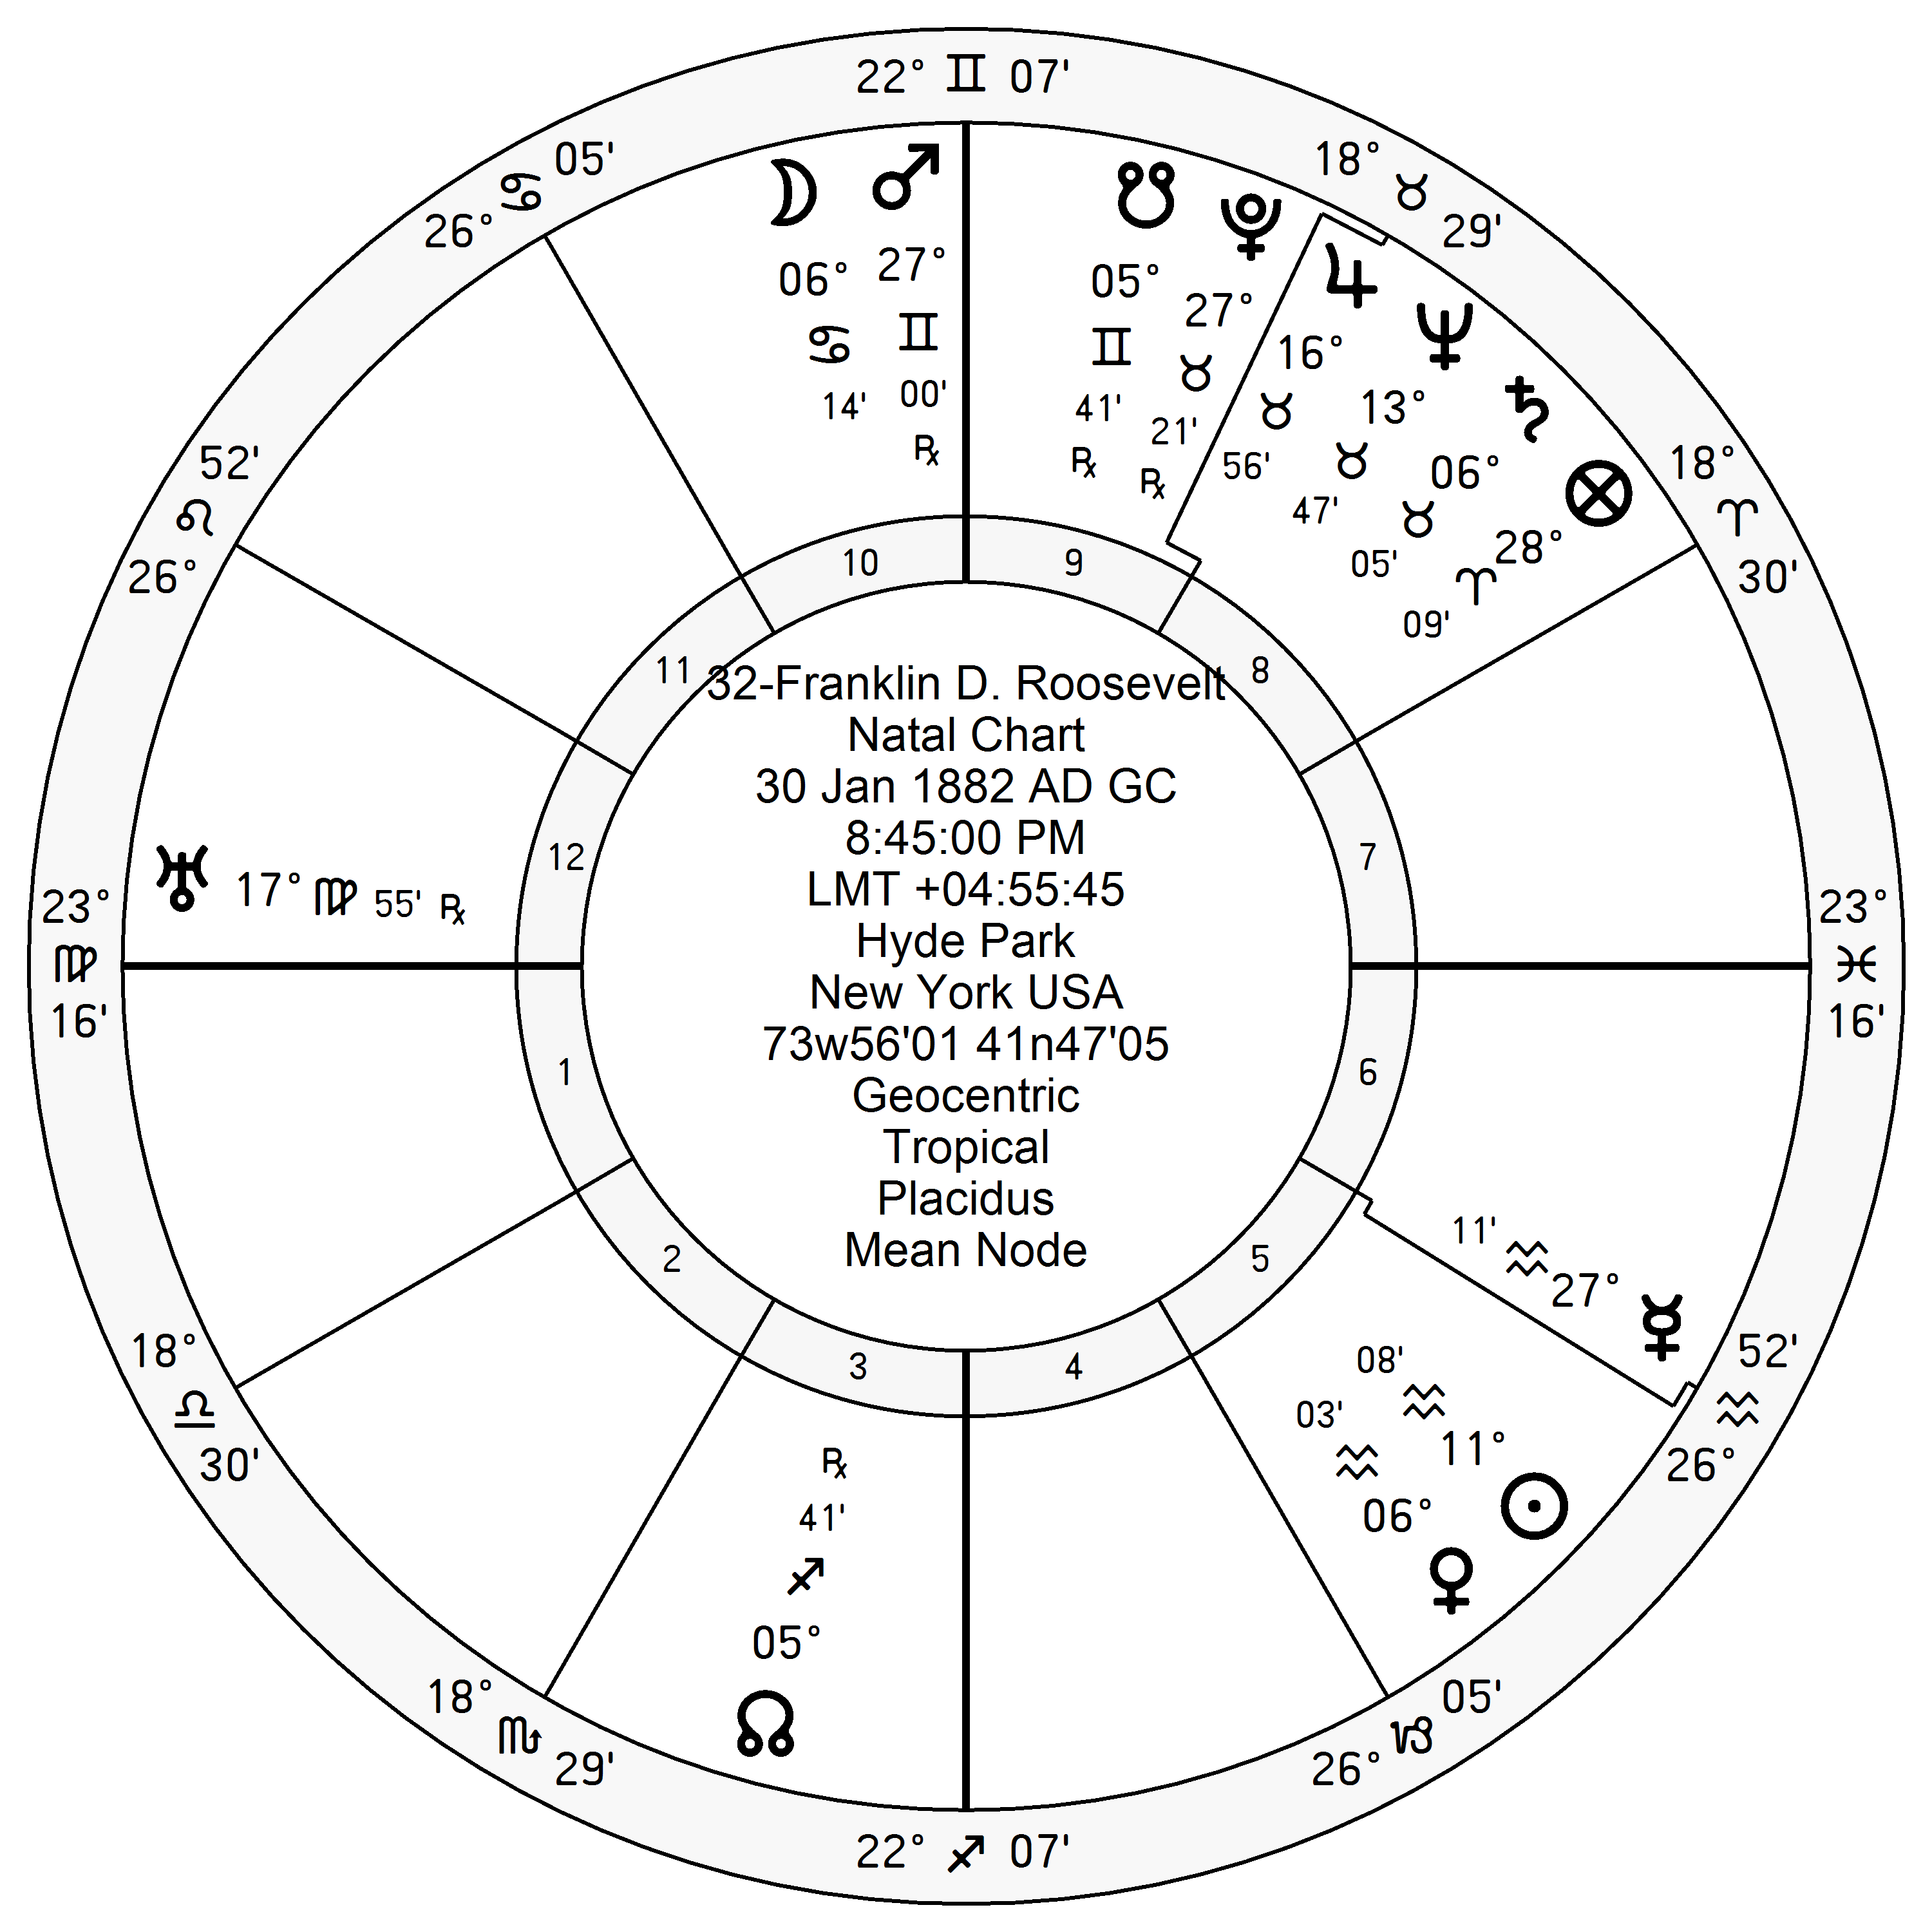
\includegraphics[width=0.9\textwidth]{charts/FDR.png}}
\fontsize{7pt}{8pt}\selectfont

\Moon\, in domicile \Sextile\, P10, P1; in N10 \Square\, N1 \\
\Mars\, \Sextile\, P10, in N10 partile \Trine\, dispositor

\column{0.48\textwidth}
\vspace{-1em}
{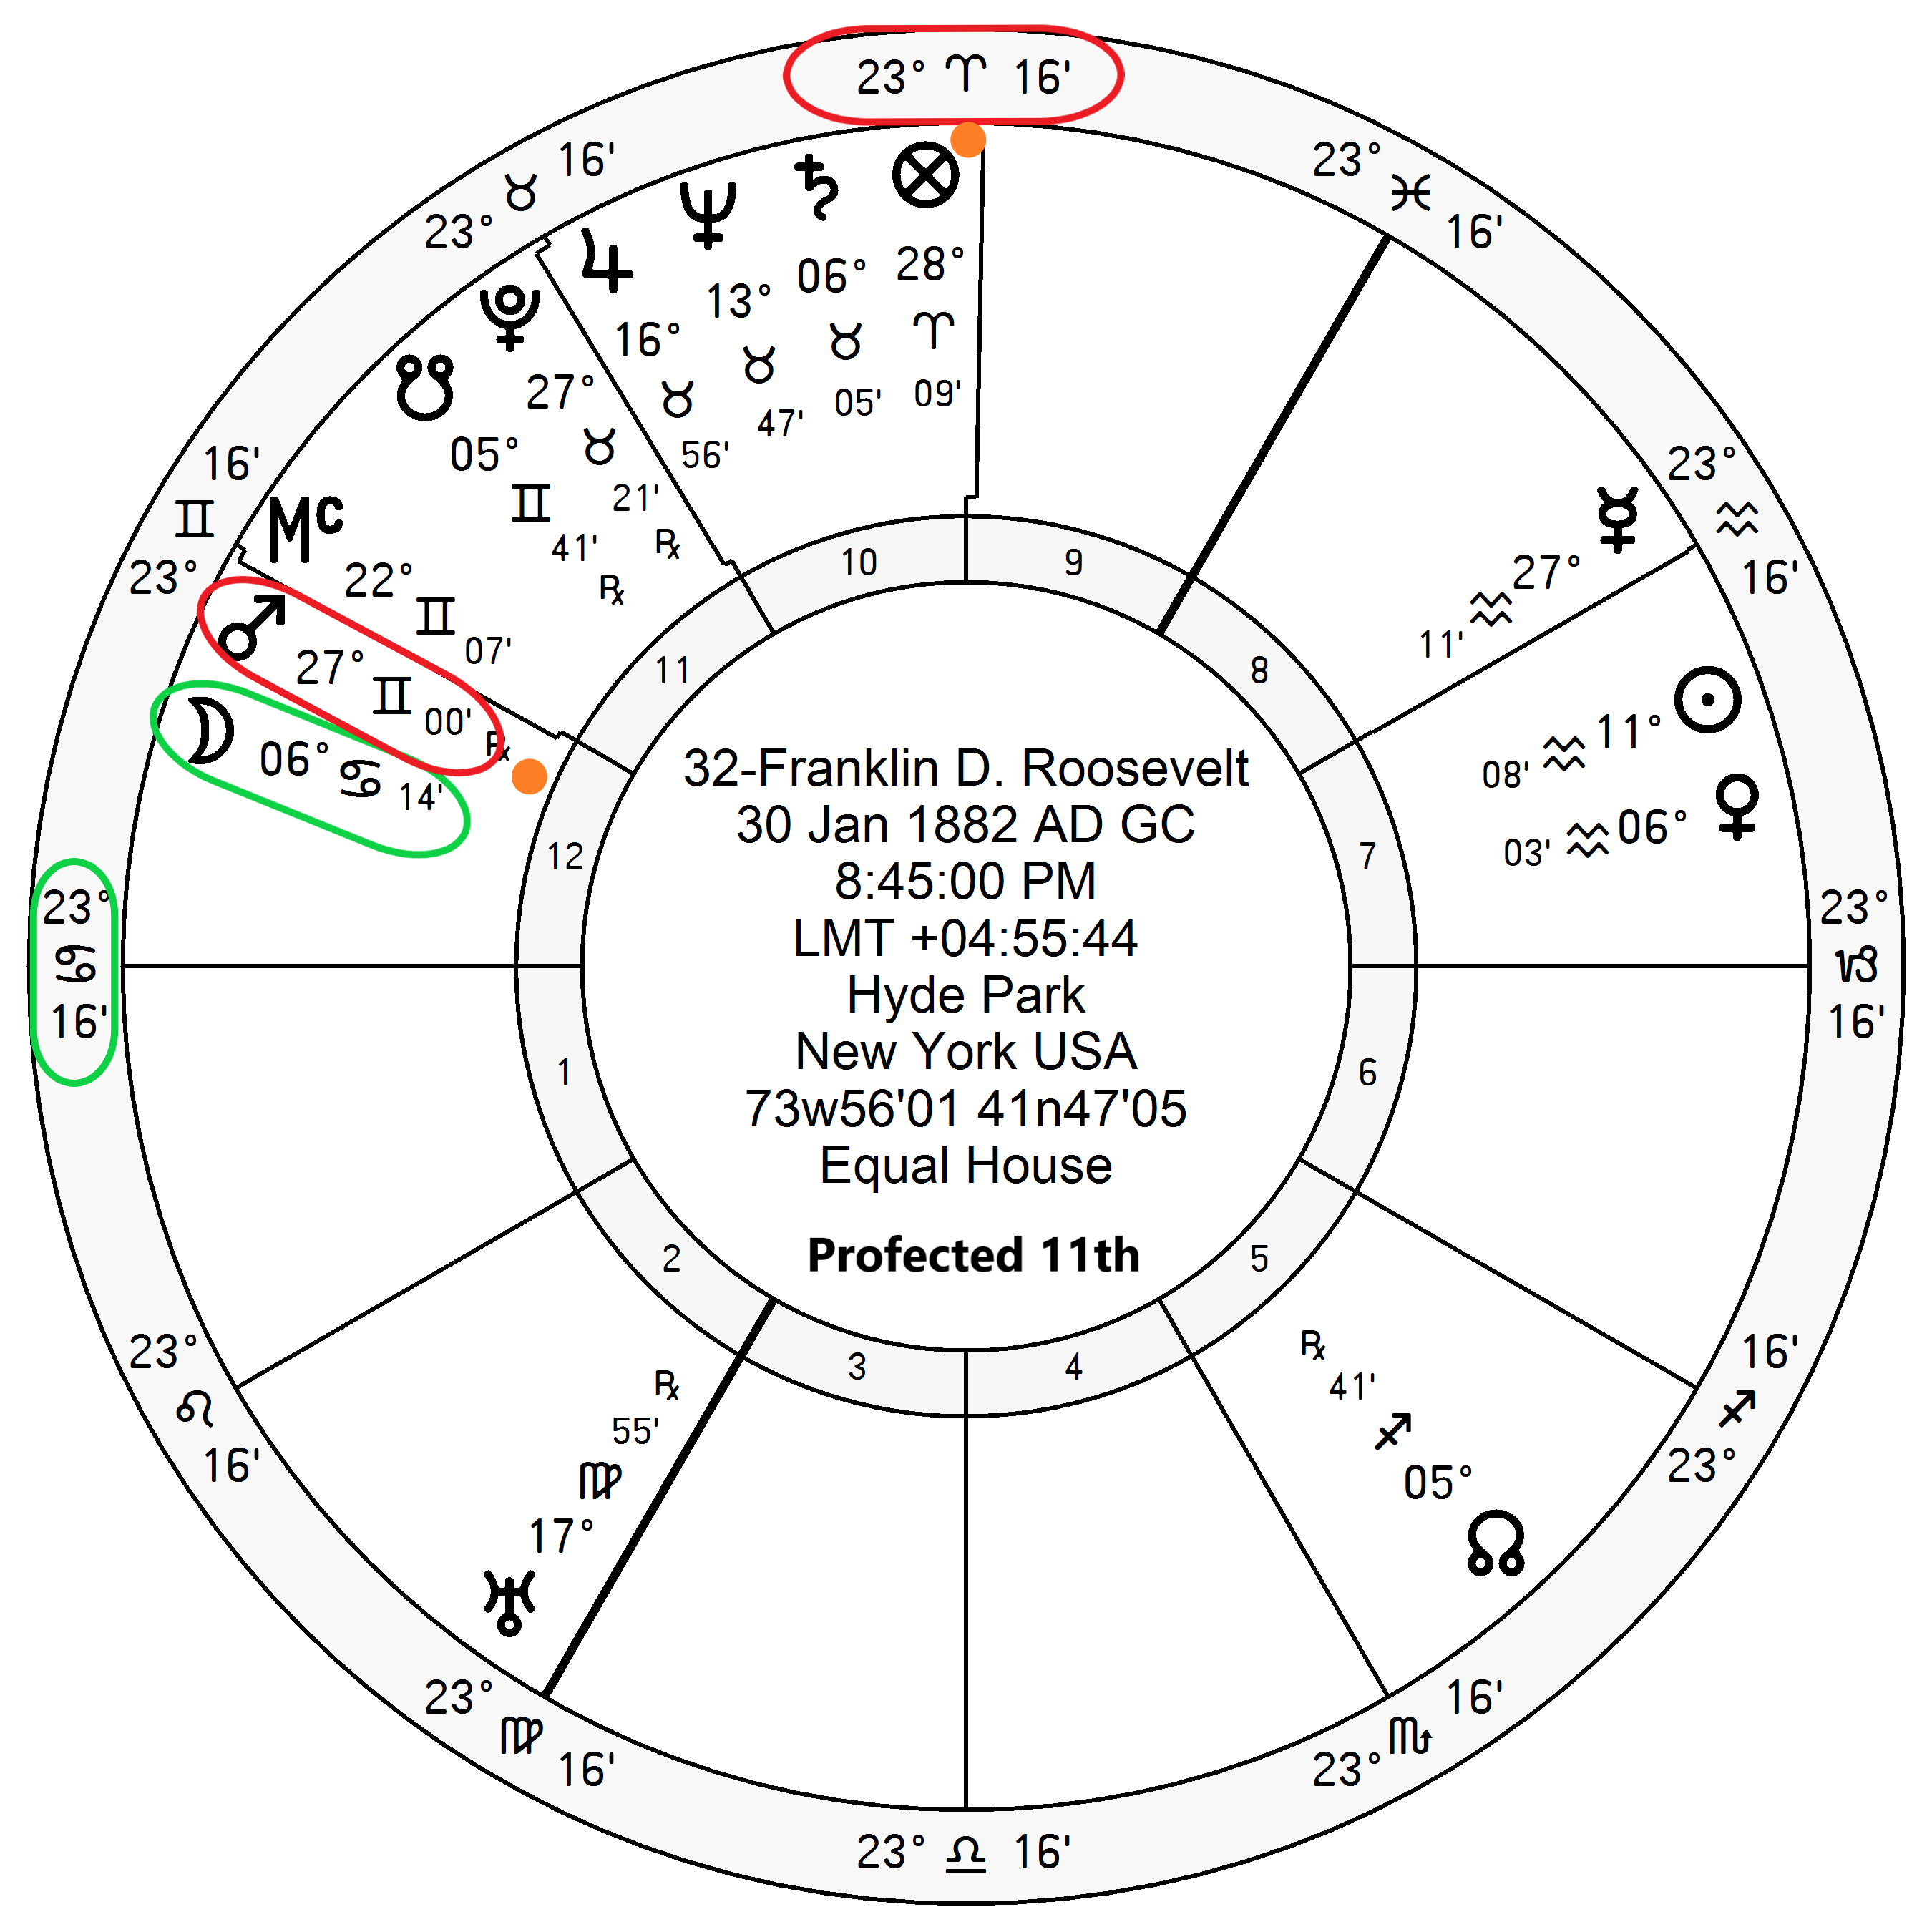
\includegraphics[width=0.9\textwidth]{charts/FDR-Prof-11th.png}}
\textbf{\dgreen P1}=N11
	$\Rightarrow$ \Moon\, (domicile) $\Rightarrow$ \textbf{\dgreen P12/N10} \\
\textbf{\red P10=N8}
	$\Rightarrow$  \Mars\,\Retrograde\, $\Rightarrow$ \textbf{\dgreen P12/N10} \\
PE=\textbf{\red P10/N8}
	$\Rightarrow$  \Mars\,\Retrograde\, $\Rightarrow$   \textbf{\dgreen P12/N10}


\end{columns}
\end{frame}

% ===================================================
\begin{frame}[t]{Election November 5, 1940: Wendell Wilkie}
\small
\begin{columns}[T, onlytextwidth]
\column{0.48\textwidth}
\vspace{-1em}
{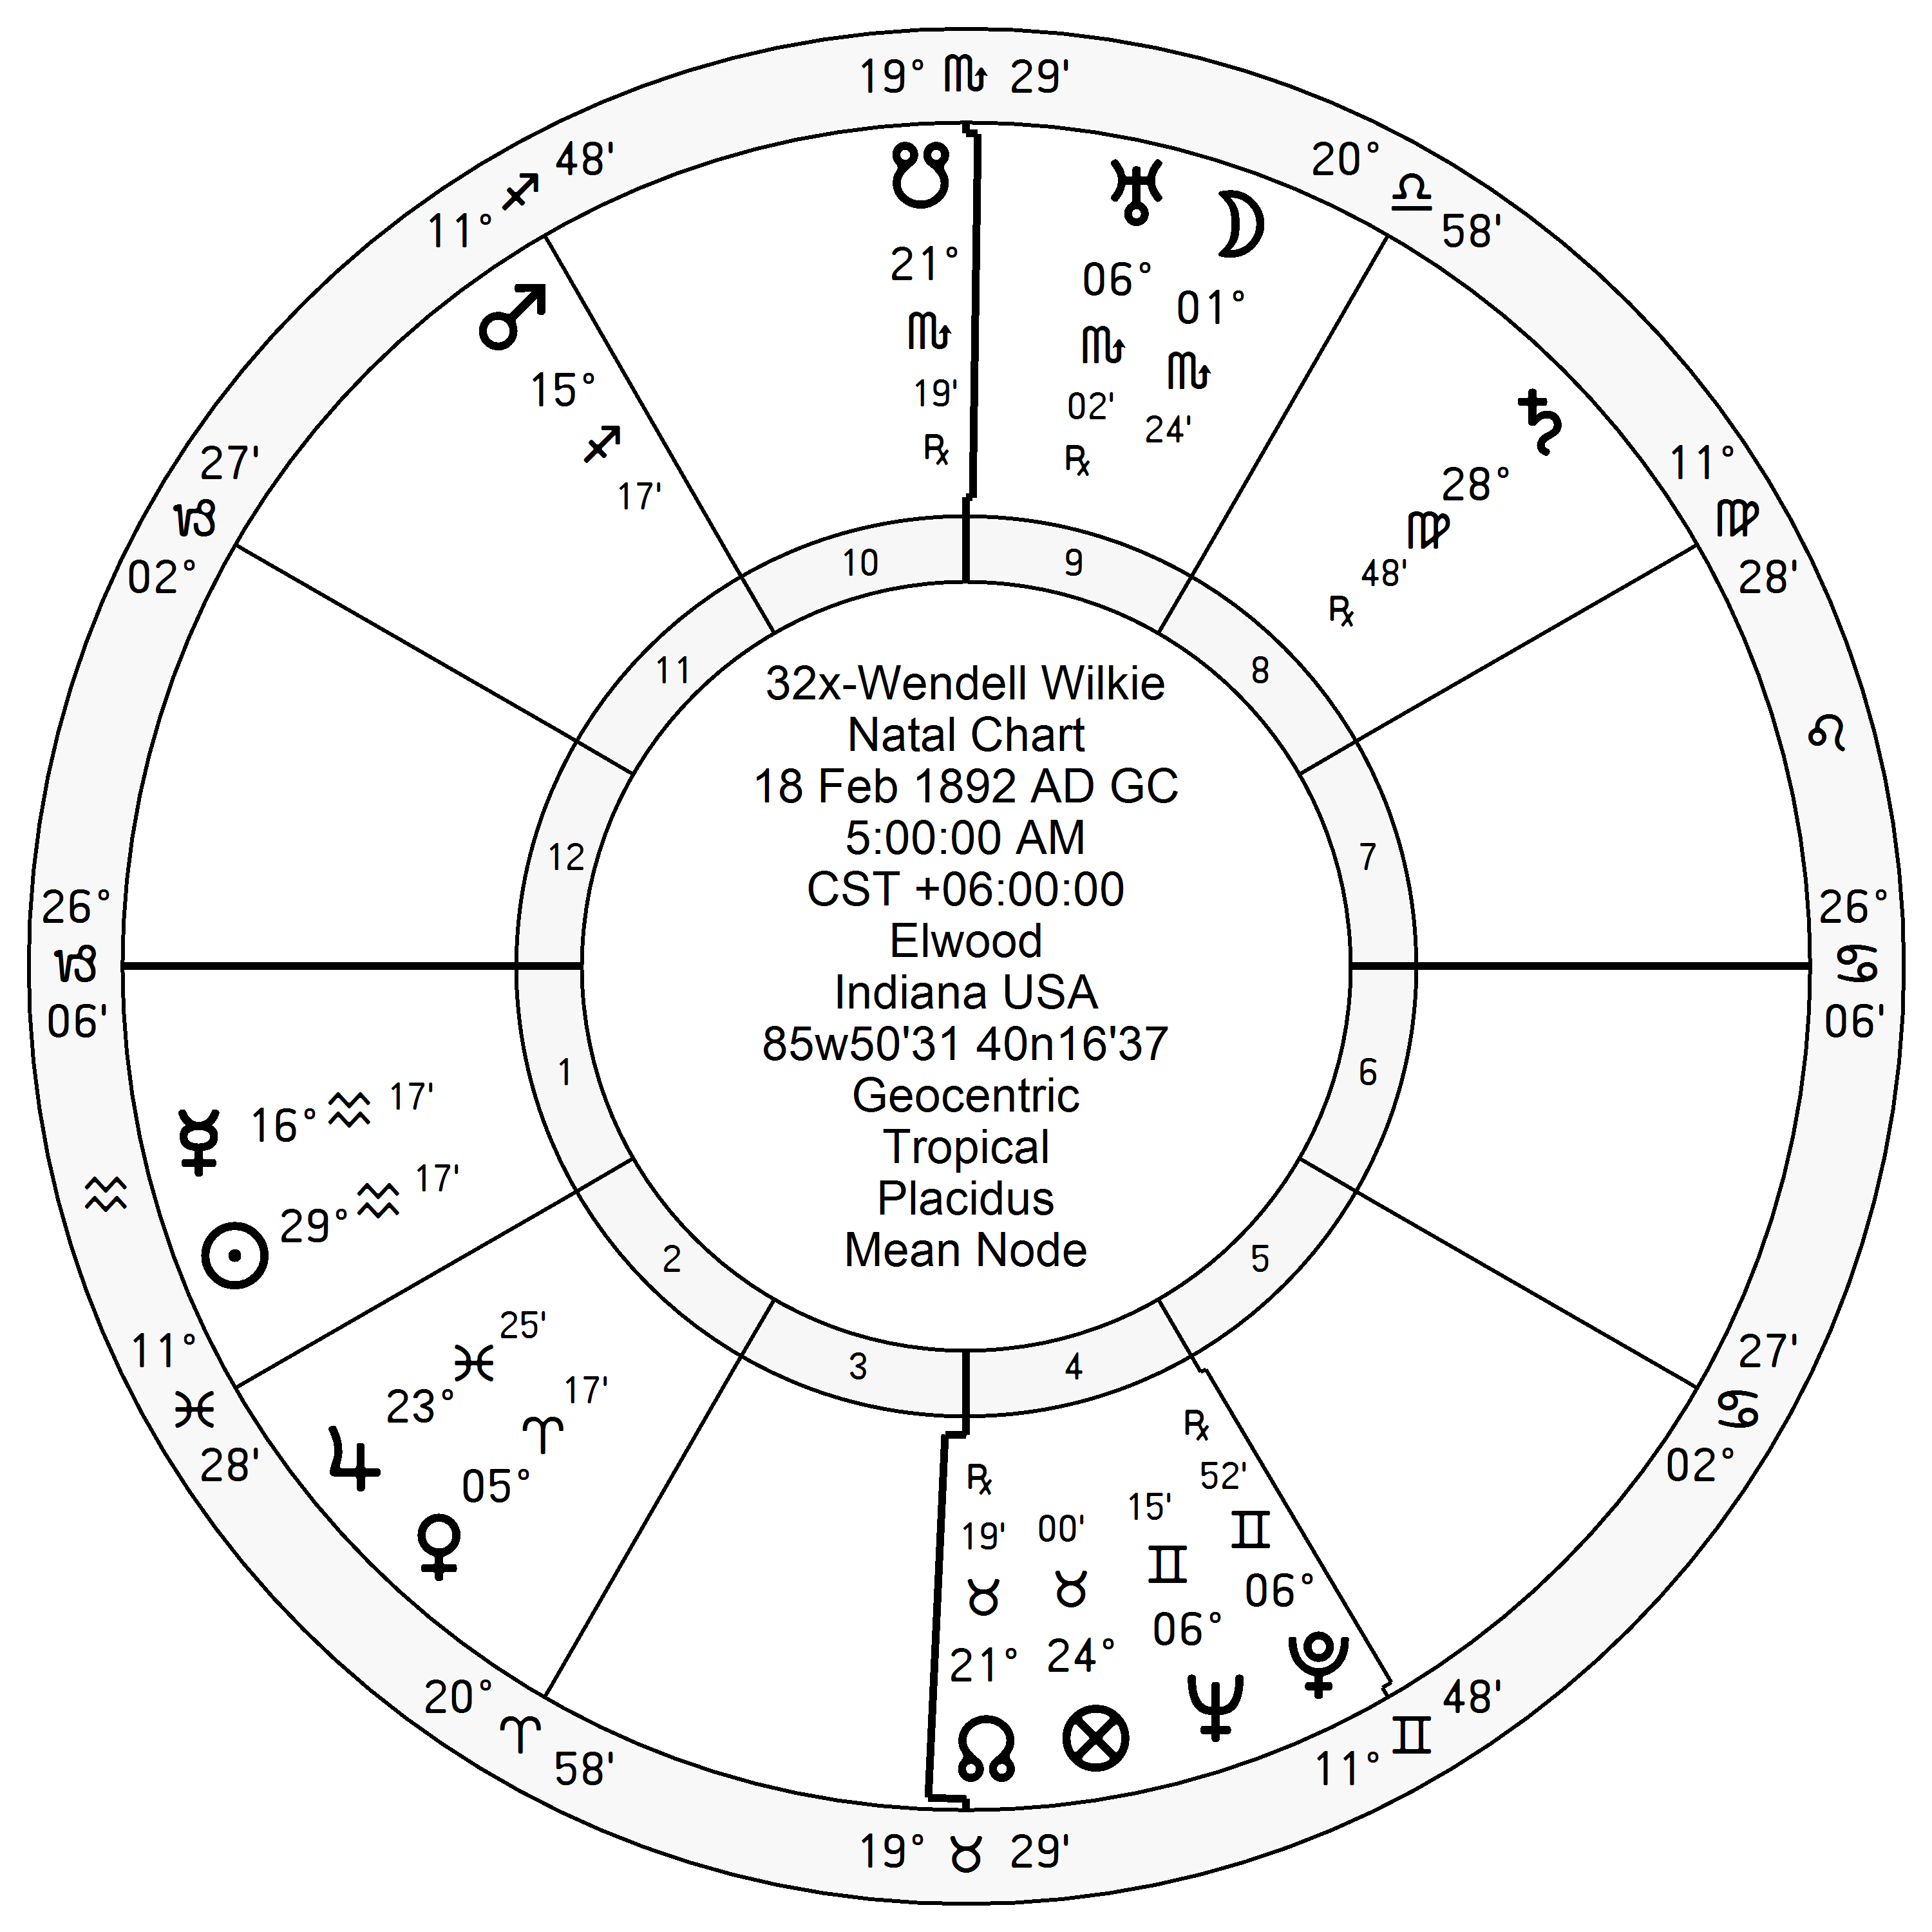
\includegraphics[width=0.9\textwidth]{charts/Wilkie.png}}
\fontsize{7pt}{8pt}\selectfont

\Saturn\, \Sextile\, N10 \\
\Venus\, \Sextile\, P1, N1 \\
\Mercury\, (USB) in P1, N1; \Square\, P10, N10 \\
\vspace{0.5em}
USB appears to weaken the square and South Node in P10/N10 doesn't help.

\column{0.48\textwidth}
\vspace{-1em}
{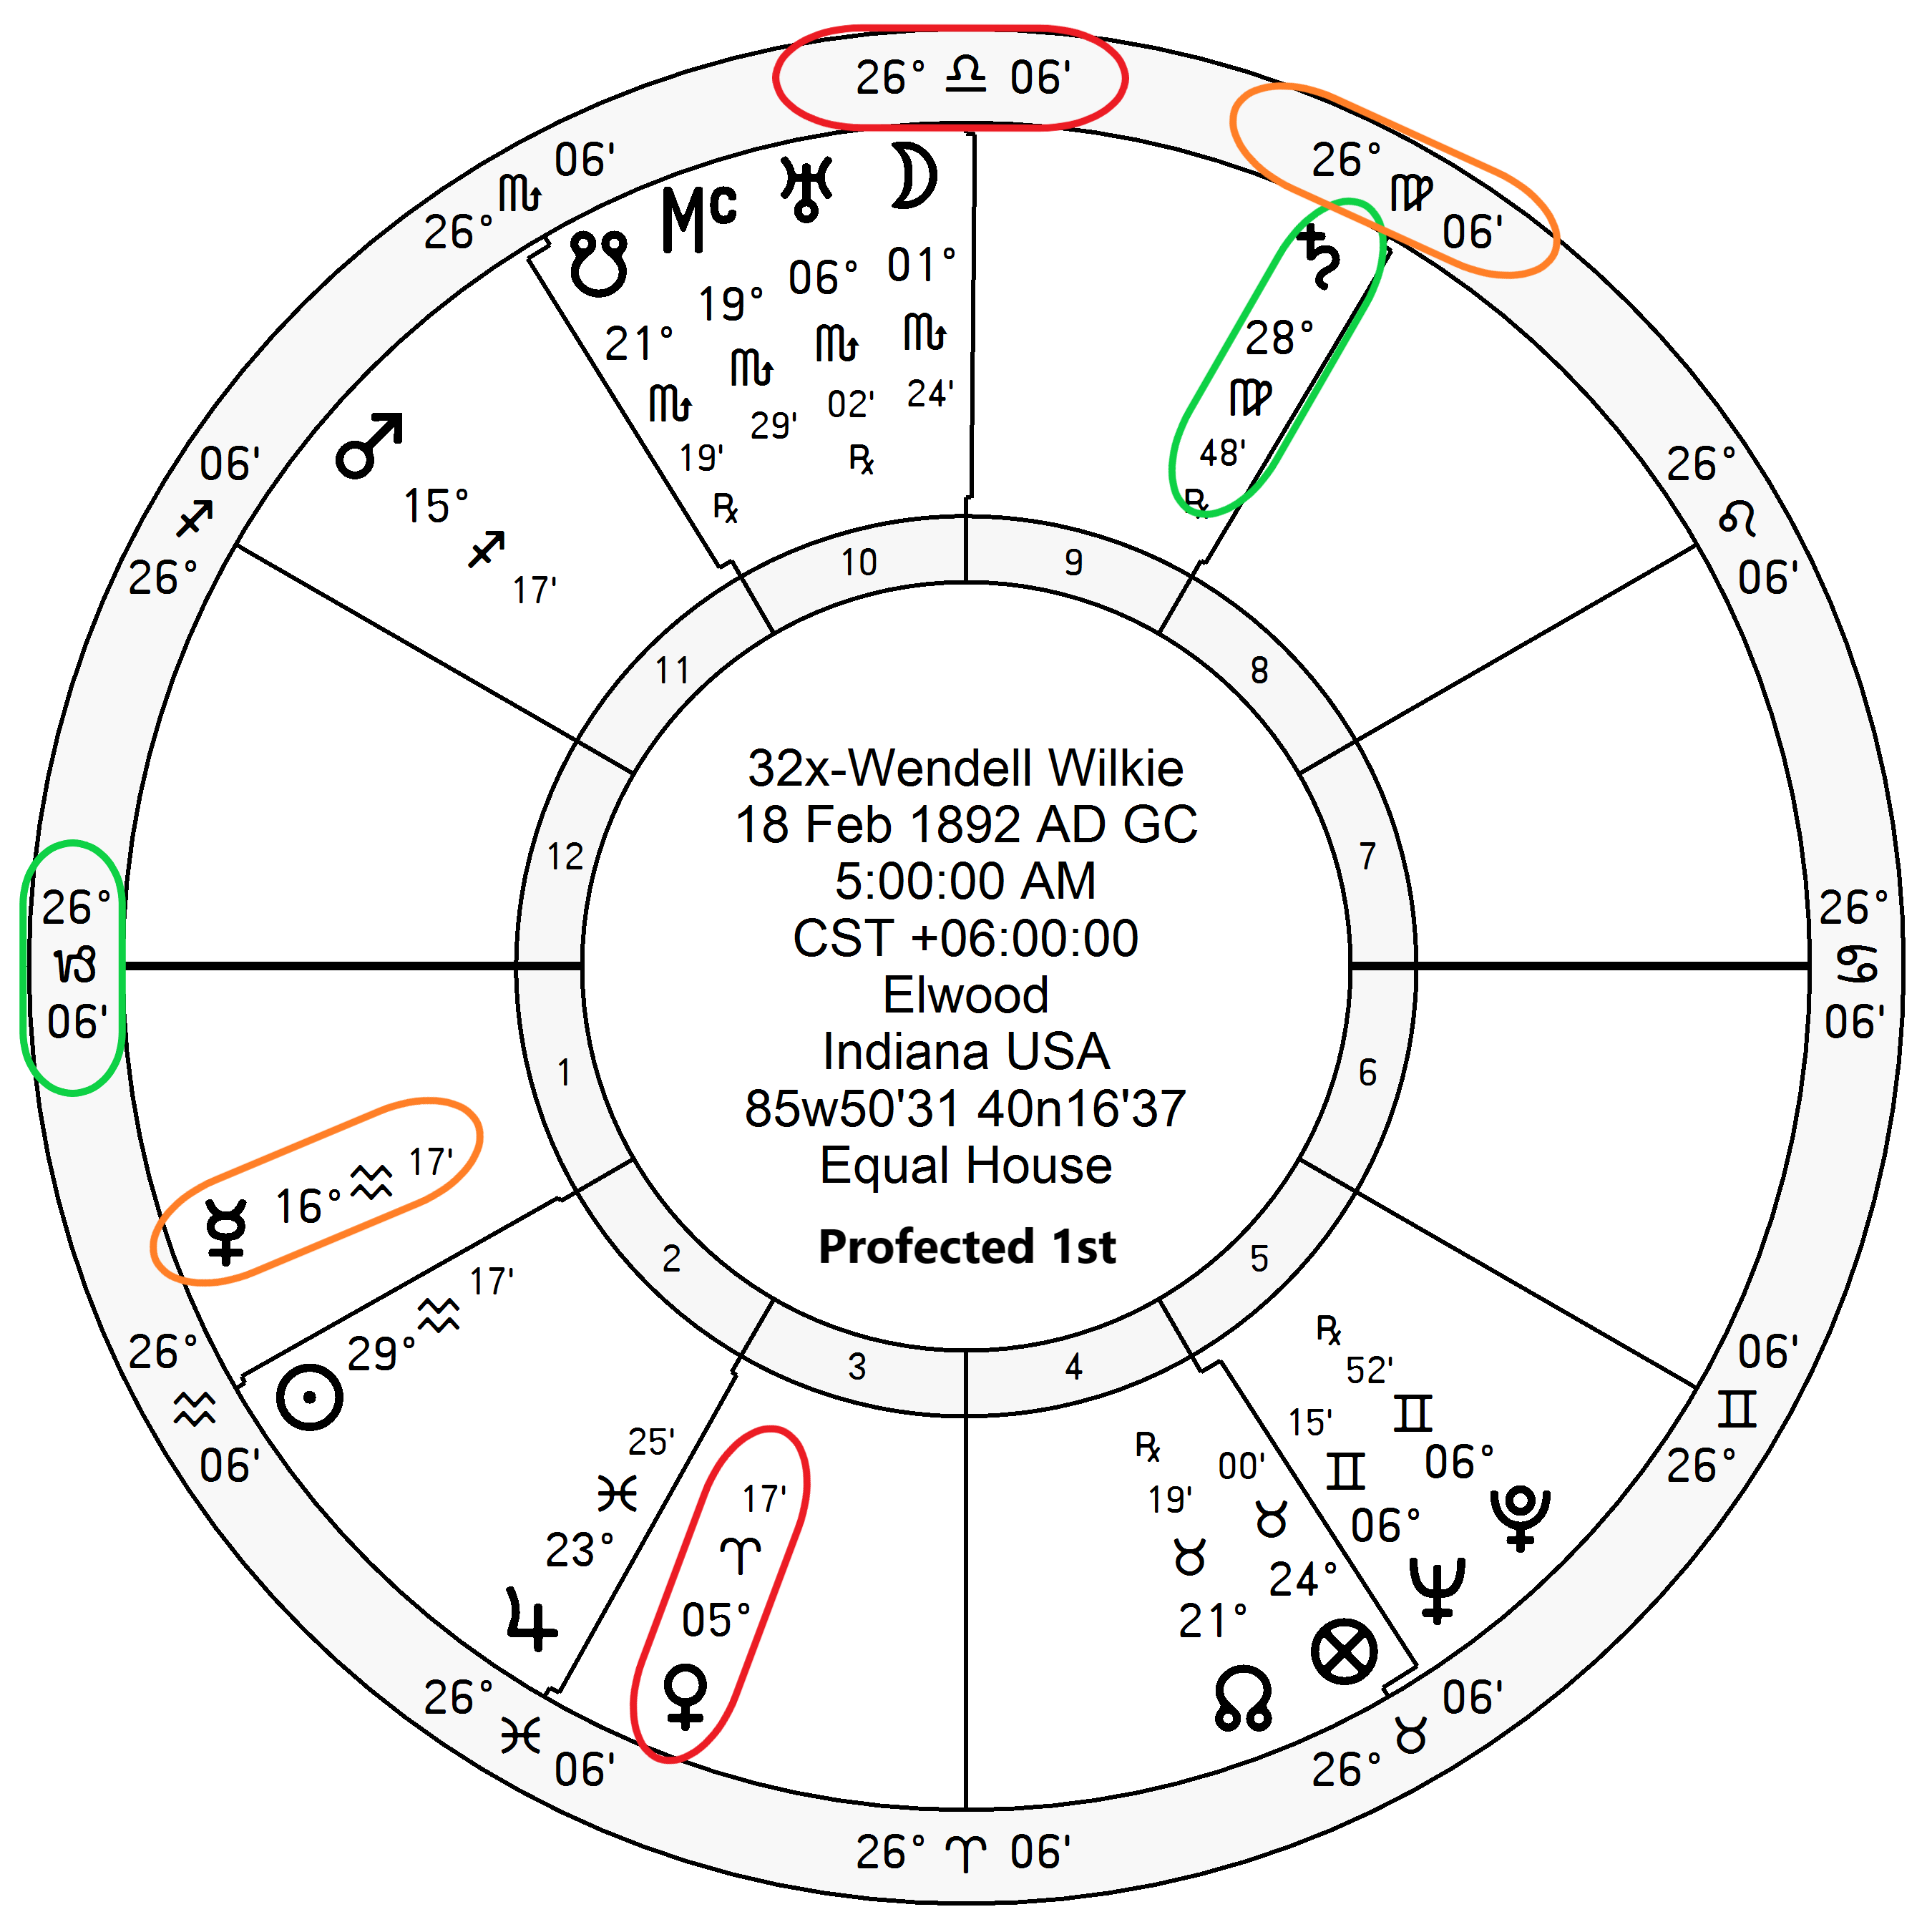
\includegraphics[width=0.9\textwidth]{charts/Wilkie-Prof-1st.png}}

\textbf{\dgreen P1=N1} 
	$\Rightarrow$ \Saturn\,\Retrograde\, $\Rightarrow$ \textbf{\red P9/N8}\\
\textbf{\red P10=N9}
	$\Rightarrow$ \Venus\, (detriment) $\Rightarrow$ P3/N2\\
PE=\textbf{\red P9/N8}
	 $\Rightarrow$ \Mercury\, (USB) $\Rightarrow$ \textbf{\dgreen P1/N1}



\end{columns}
\end{frame}

%\subsection{Election November 8, 1960: *Kennedy vs Nixon}
\begin{frame}[t]{Election November 8, 1960: *John Fitzgerald Kennedy}
\small

\begin{columns}[T, onlytextwidth]
\column{0.48\textwidth}
\vspace{-1em}
{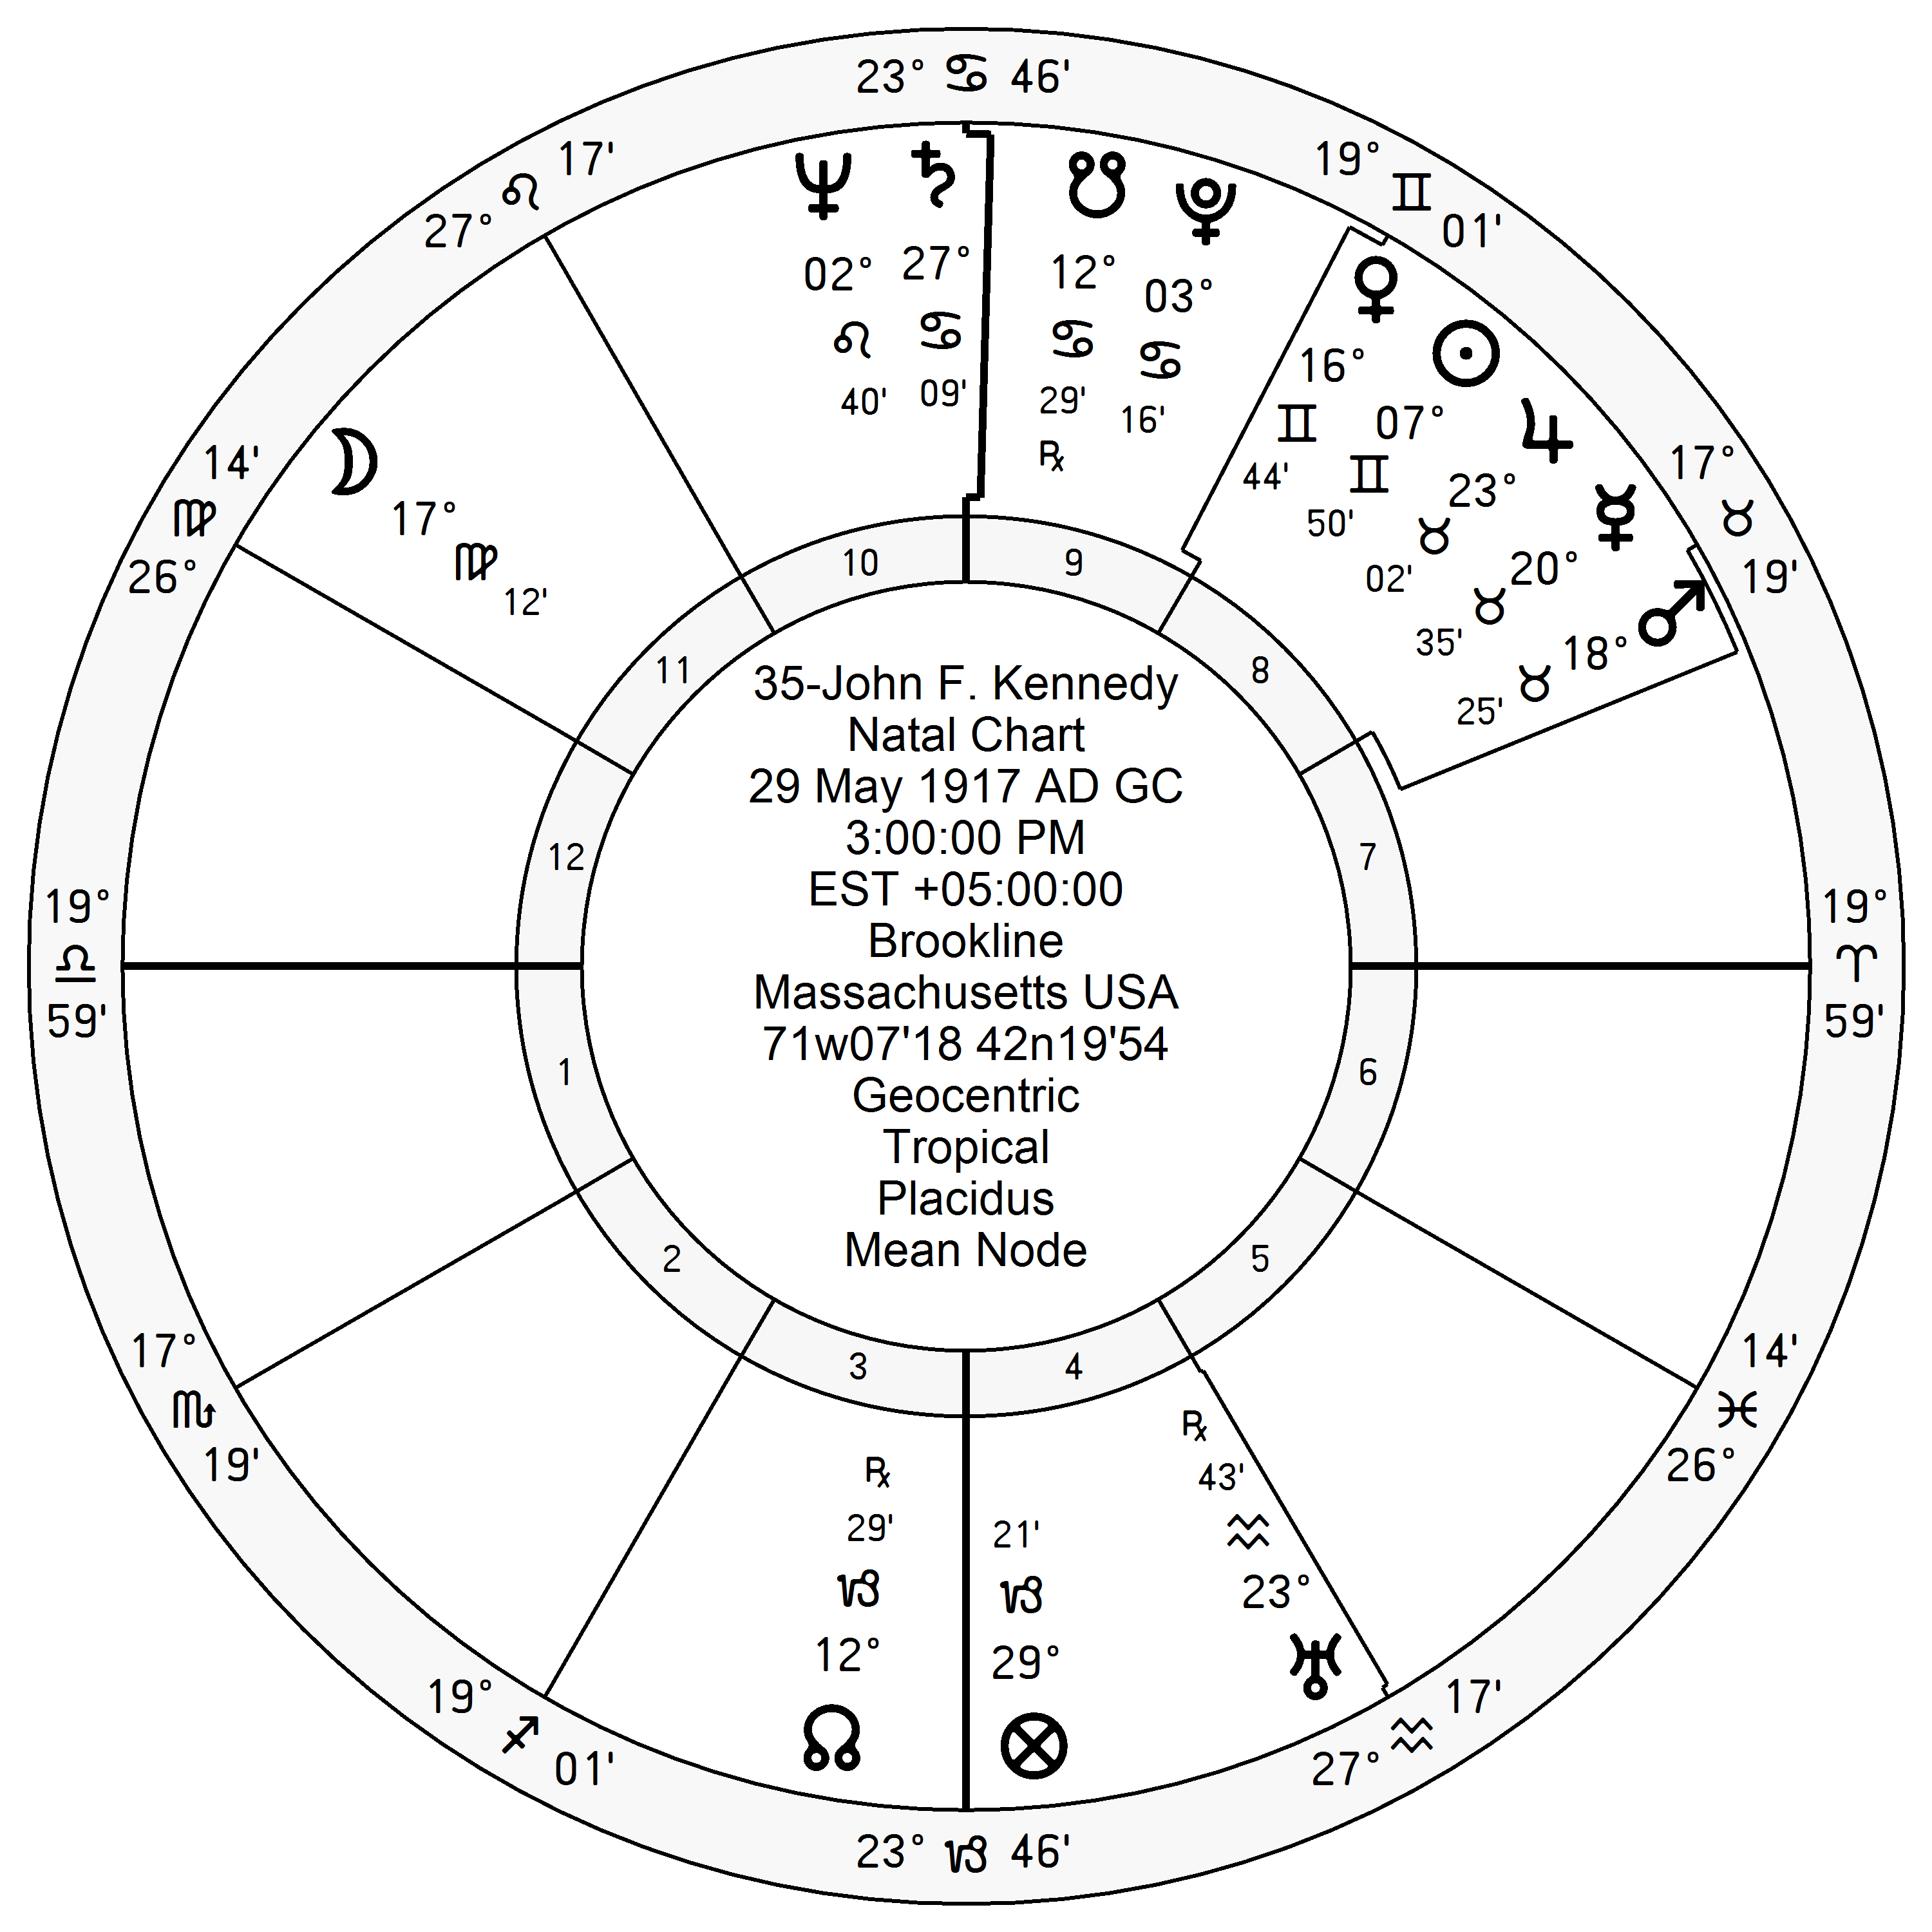
\includegraphics[width=0.9\textwidth]{charts/JFK.png}}
\fontsize{7pt}{8pt}\selectfont

\Venus\, (USB) in P1, \Square\, P10; \Sextile\, N10 \\
\Saturn\, \Sextile\, P1; in N10, \Square\, N1 \\
\vspace{0.5em}
The charts look weaker than Nixon's; possible Kennedy won because \Saturn\, as the exaltation ruler of the 1st, in the N10, with dispositor in the 11th `promises' a rise?


\column{0.48\textwidth}
\vspace{-1em}
{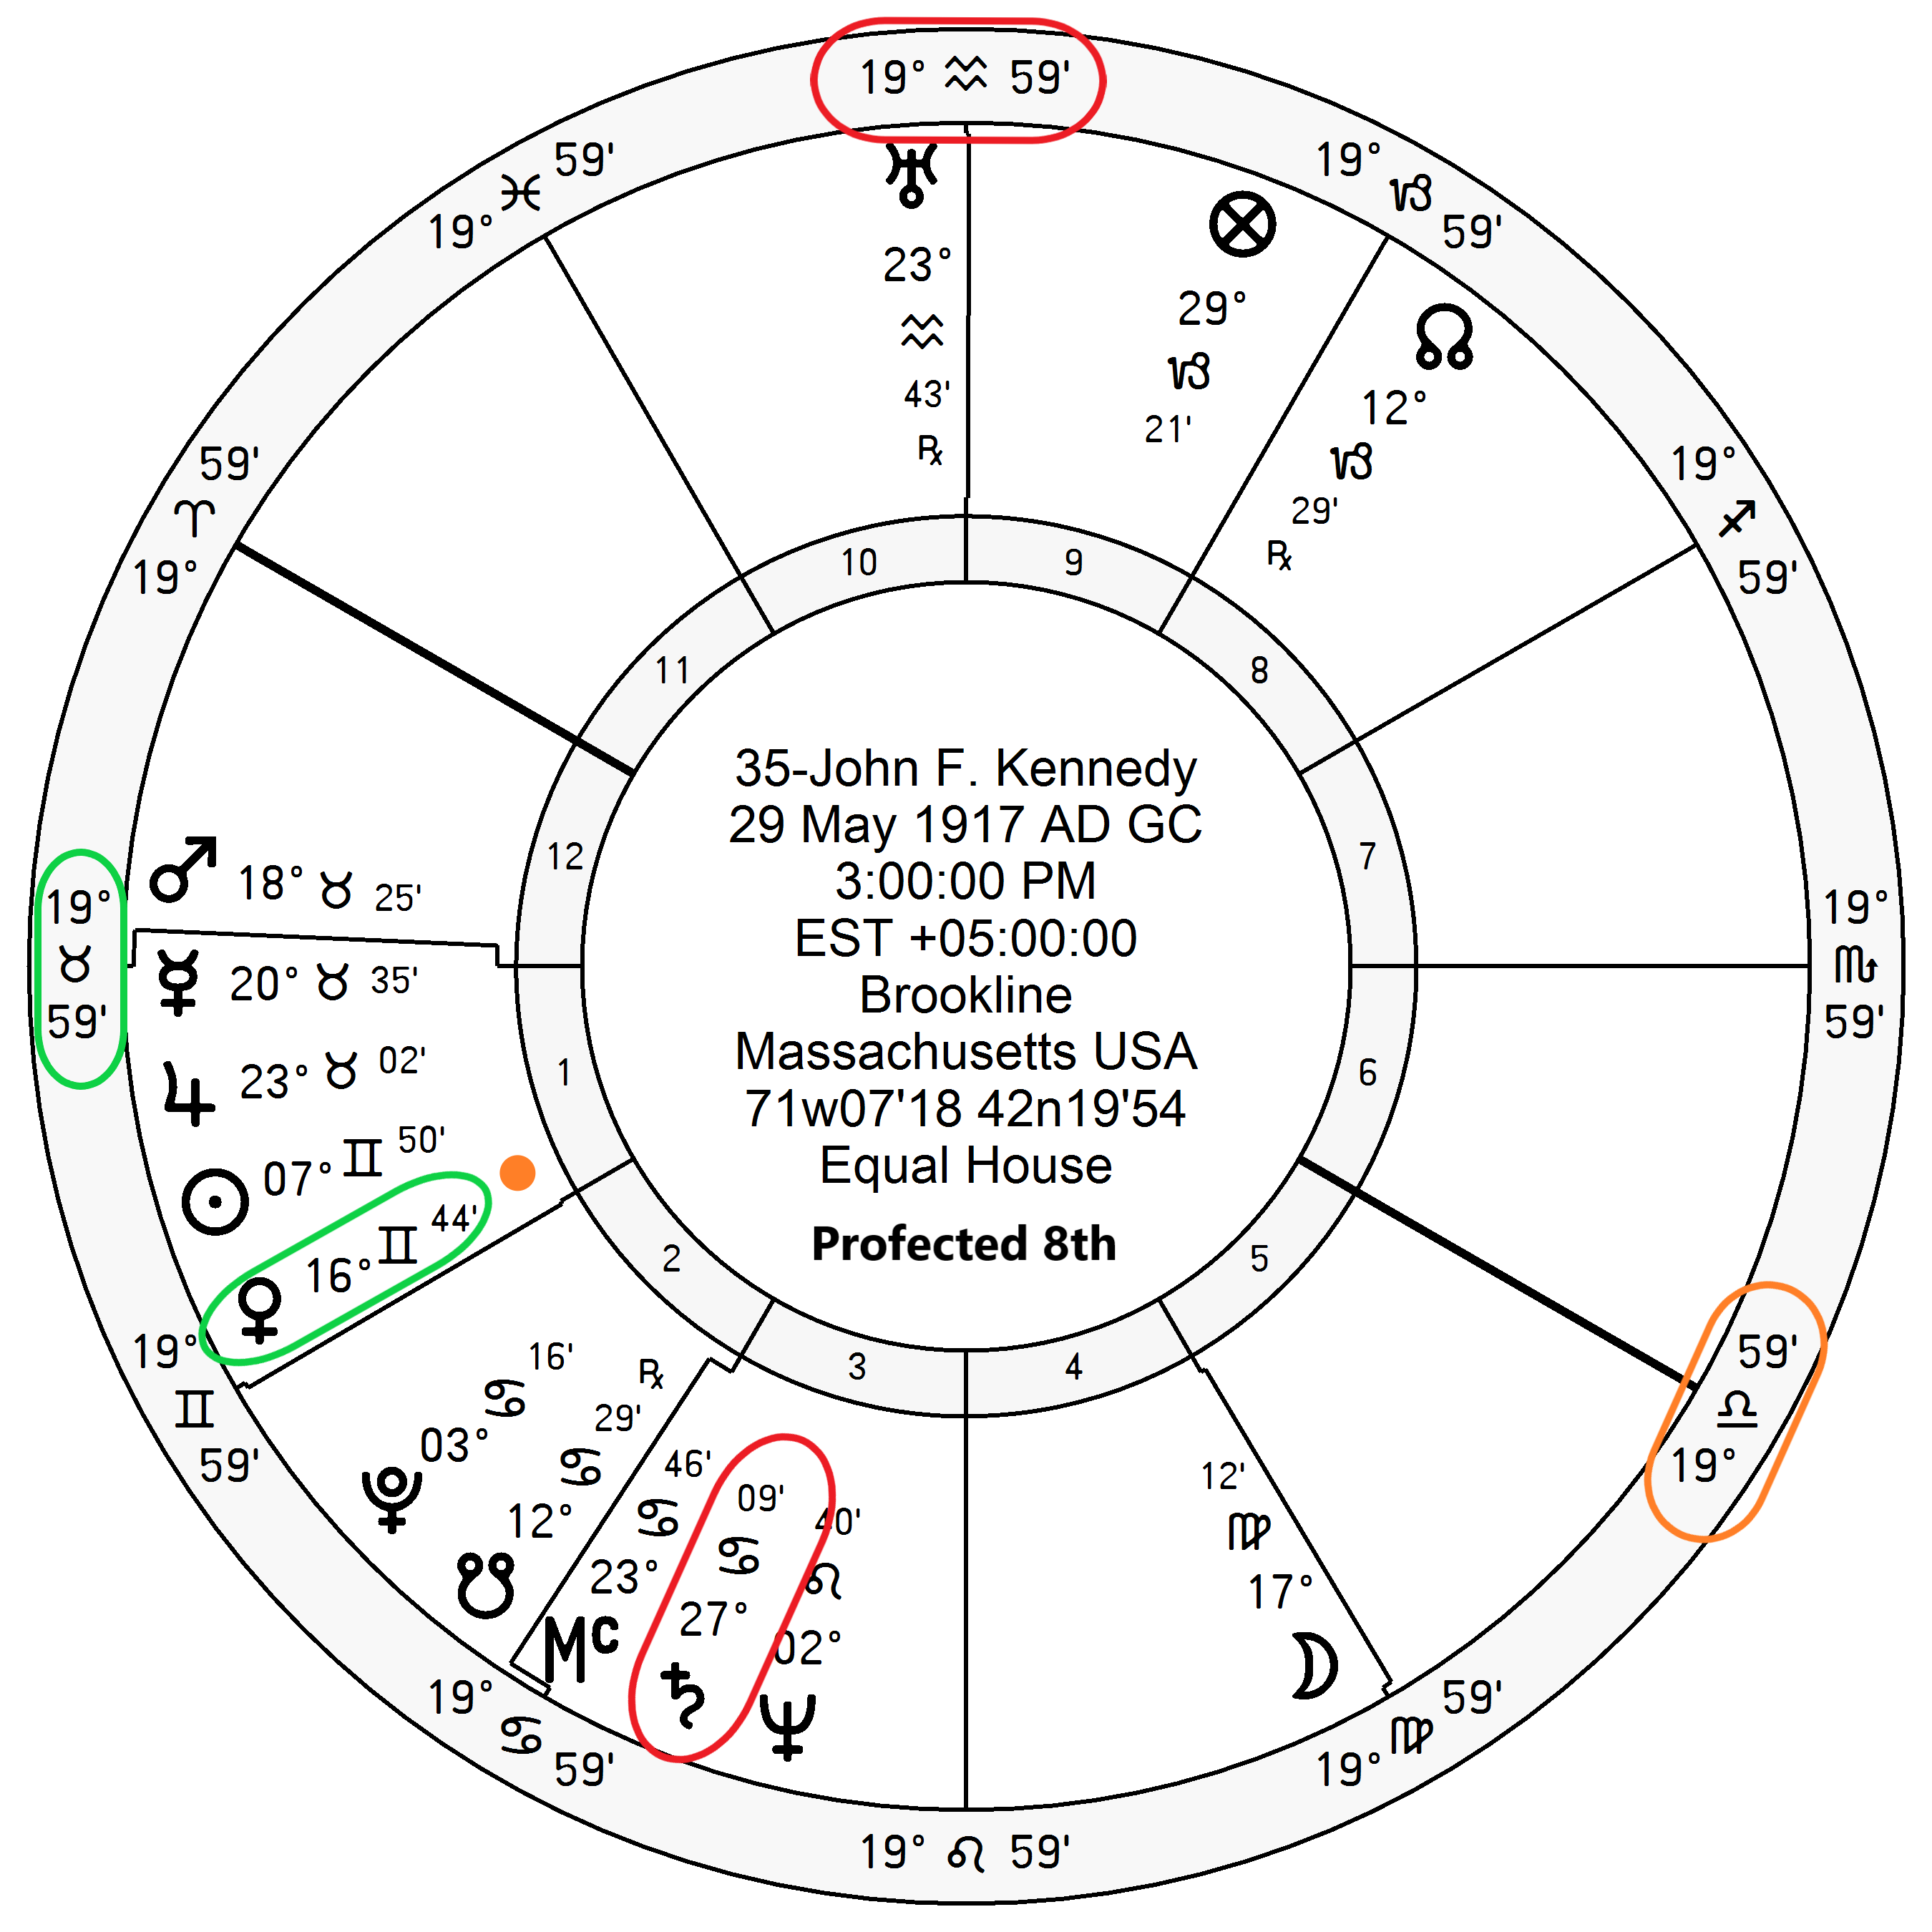
\includegraphics[width=0.9\textwidth]{charts/JFK-Prof-8th.png}}
\fontsize{7pt}{8pt}\selectfont

\textbf{\dgreen P1=N8}
	$\Rightarrow$ \Venus\, (USB) $\Rightarrow$ \textbf{\dgreen P1/N8} \\
\textbf{\red P10}=N5
	$\Rightarrow$  \Saturn\, $\Rightarrow$ P3/\textbf{\red N10} \\
PE=P6/\textbf{\dgreen N1}
	$\Rightarrow$  \Venus\, $\Rightarrow$   \textbf{\dgreen P1/N1}


\end{columns}
\end{frame}

% ===================================================
\begin{frame}[t]{Election November 8, 1960: Richard Nixon}
\small
\begin{columns}[T, onlytextwidth]
\column{0.48\textwidth}
\vspace{-1em}
{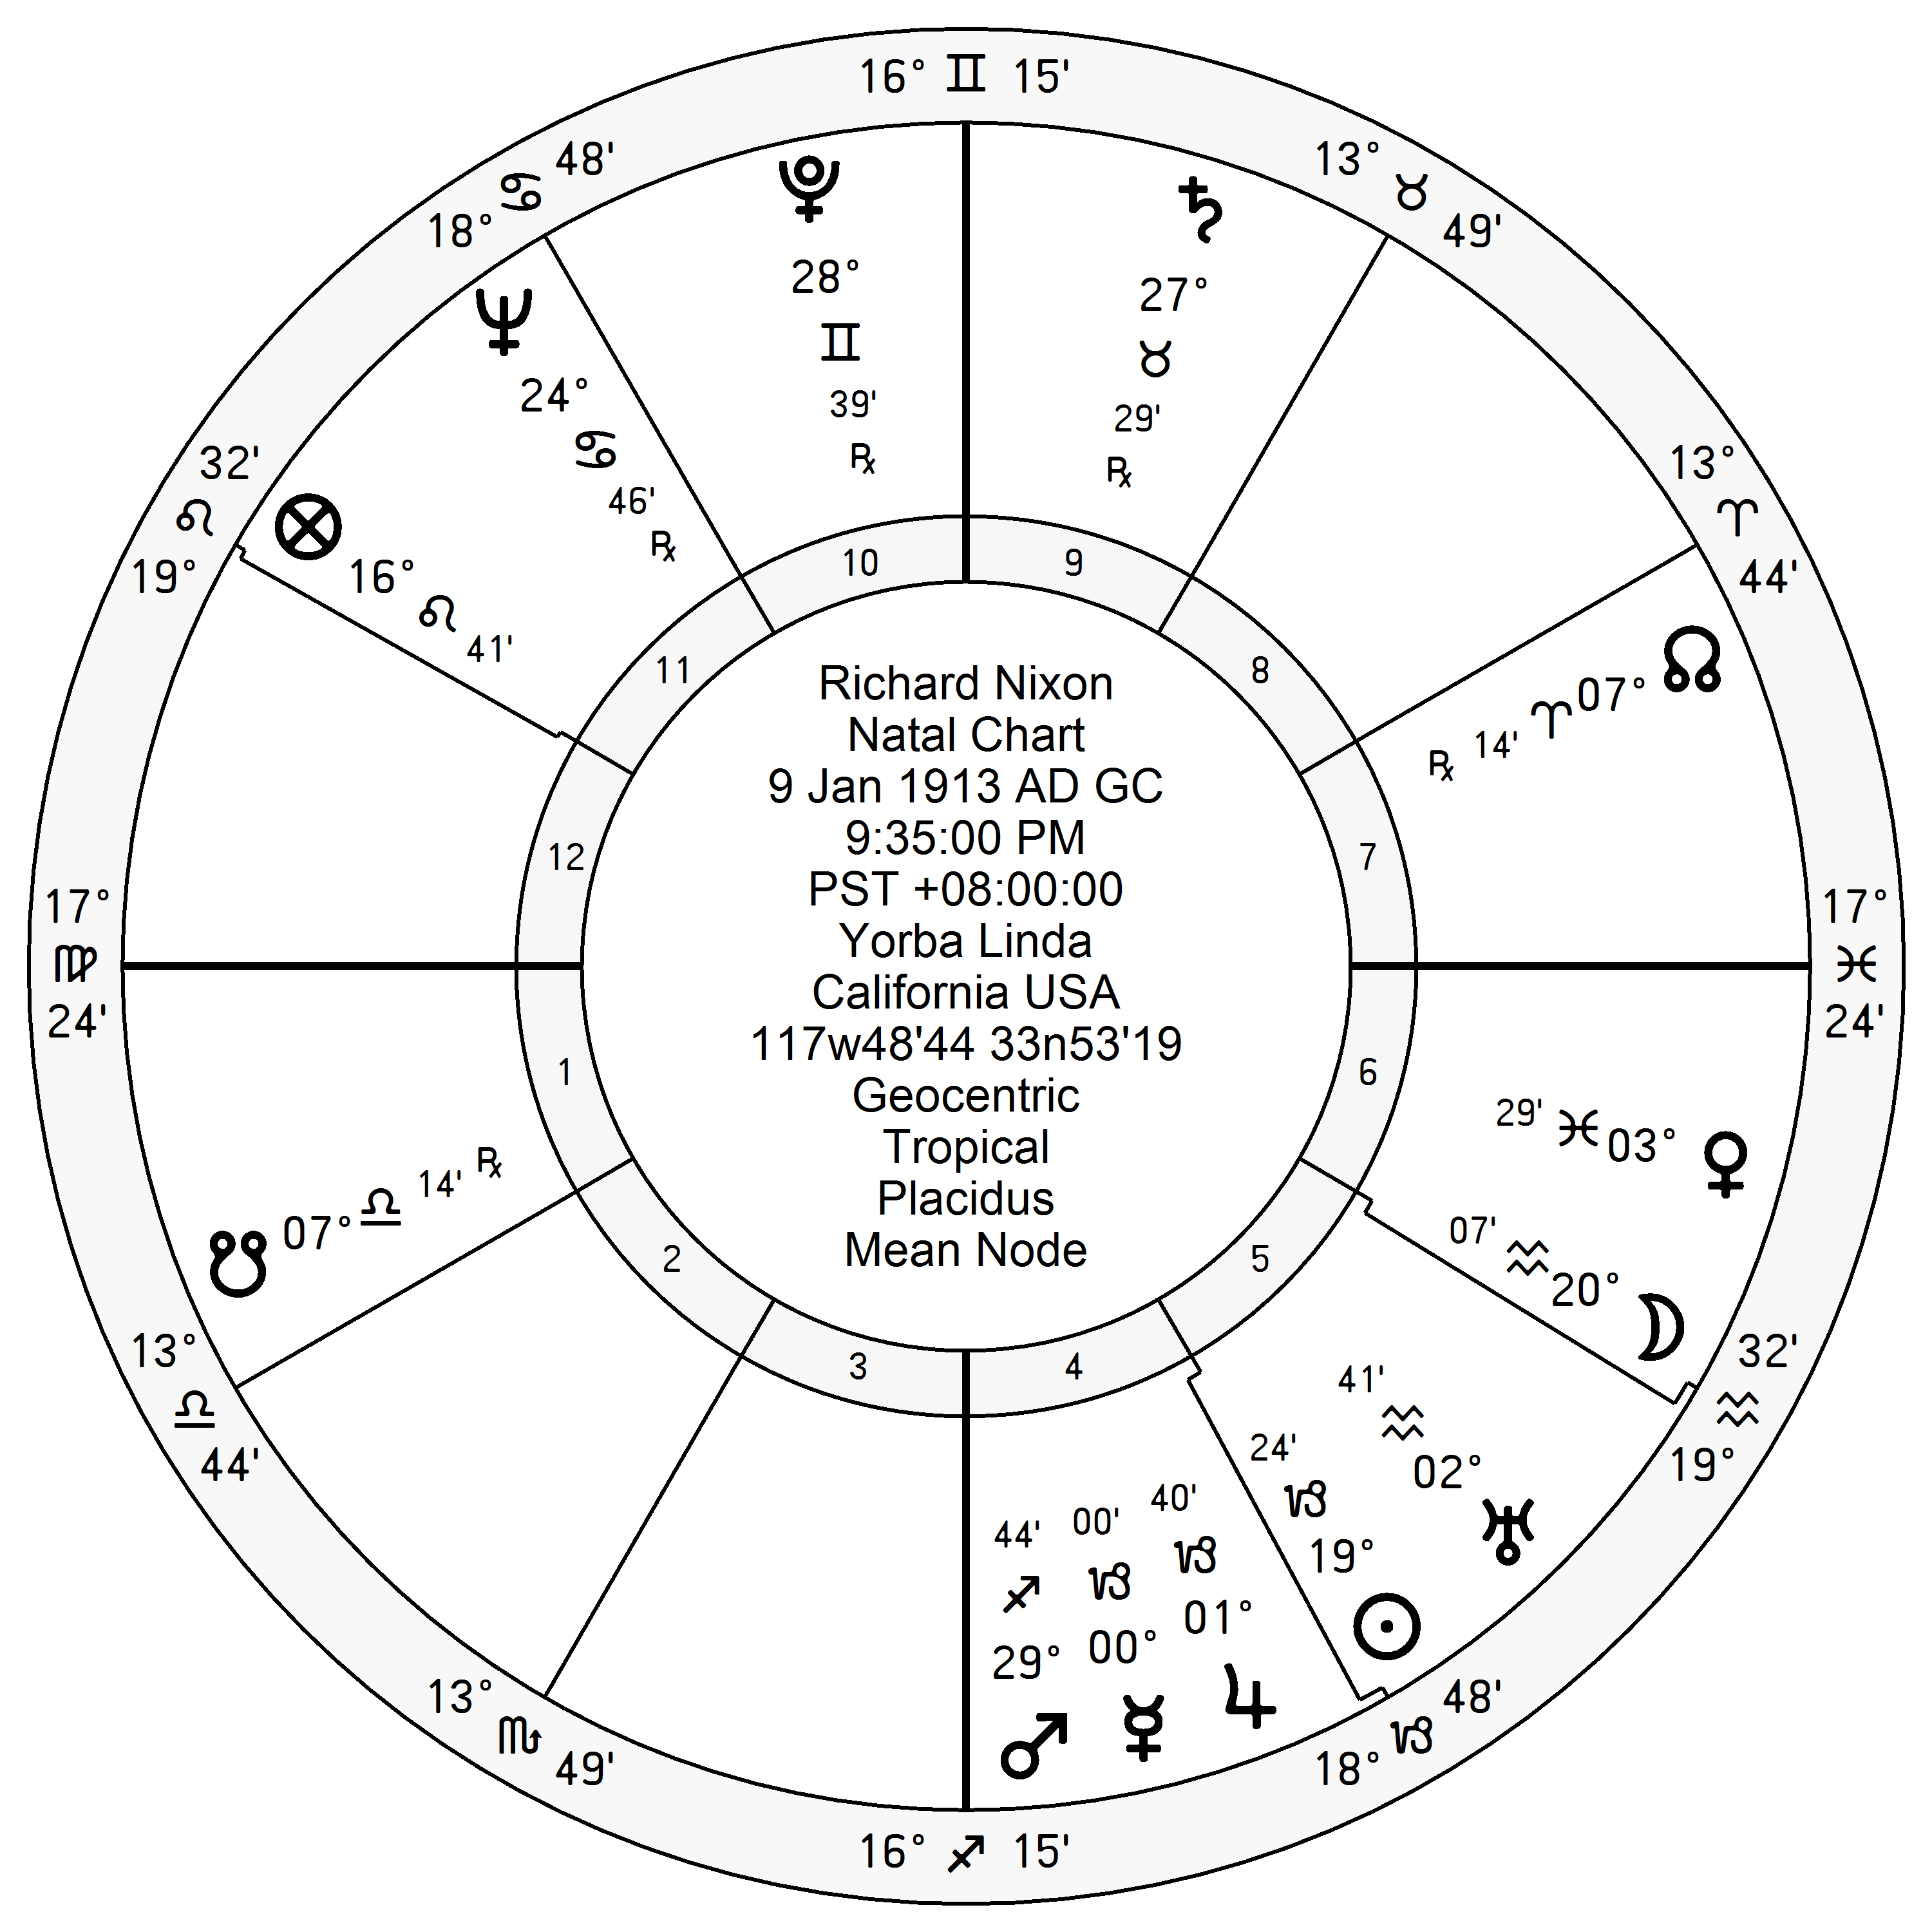
\includegraphics[width=0.9\textwidth]{charts/Nixon.png}}
\fontsize{7pt}{8pt}\selectfont

\Sun\, \Trine\, P10, \Trine\, N1 \\
\Venus\, \Square\, P10, \Opposition\, N1; \Trine\, N10 \\

\column{0.48\textwidth}
\vspace{-1em}
{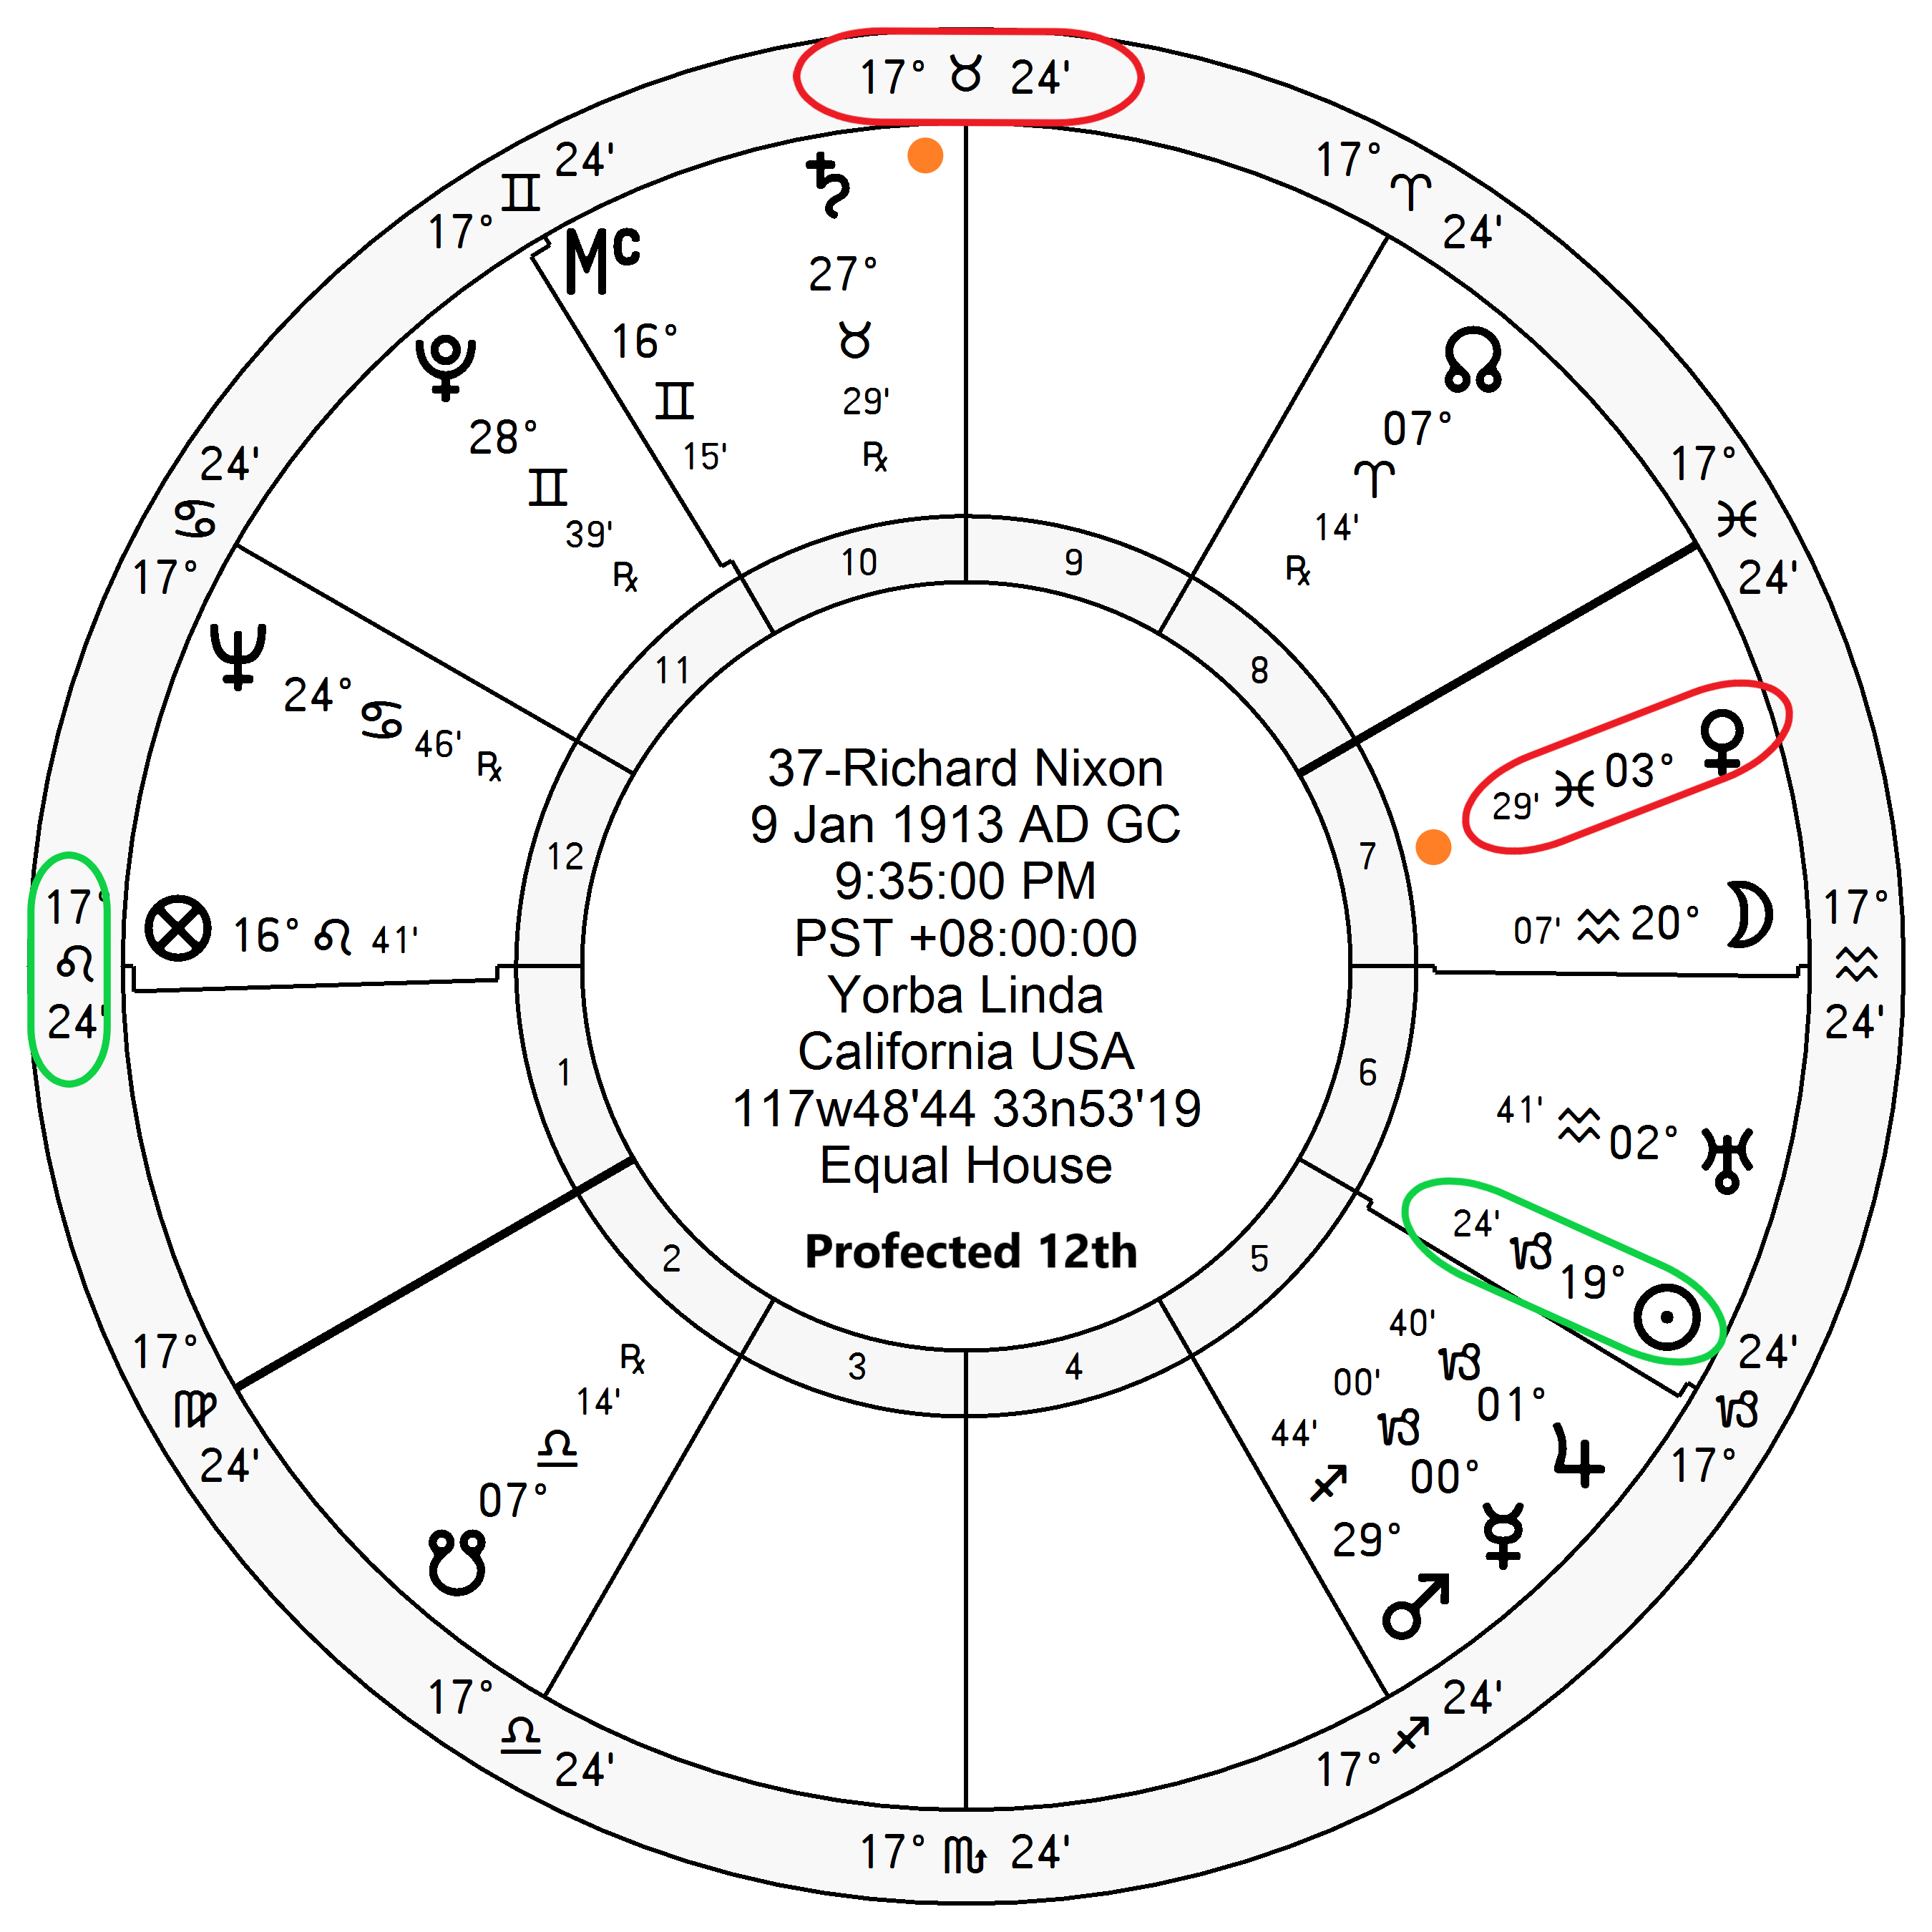
\includegraphics[width=0.9\textwidth]{charts/Nixon-Prof-12th.png}}
\fontsize{8pt}{9pt}\selectfont

\textbf{\dgreen P1=N12} 
	$\Rightarrow$ \Sun\, $\Rightarrow$ \textbf{\dgreen P6}/N5\\
\textbf{\red P10=N9}
	$\Rightarrow$ \Venus\, $\Rightarrow$ \textbf{\dgreen P7/N6}\\
PE=\textbf{\red P10/N9}
	 $\Rightarrow$ \Venus\, $\Rightarrow$ \textbf{\dgreen P7/N6}

\end{columns}
\end{frame}

%\subsection{Election November 7, 1972: *Nixon vs McGovern}
\begin{frame}[t]{Election November 7, 1972: *Richard Nixon}
\small

\begin{columns}[T, onlytextwidth]
\column{0.48\textwidth}
\vspace{-1em}
{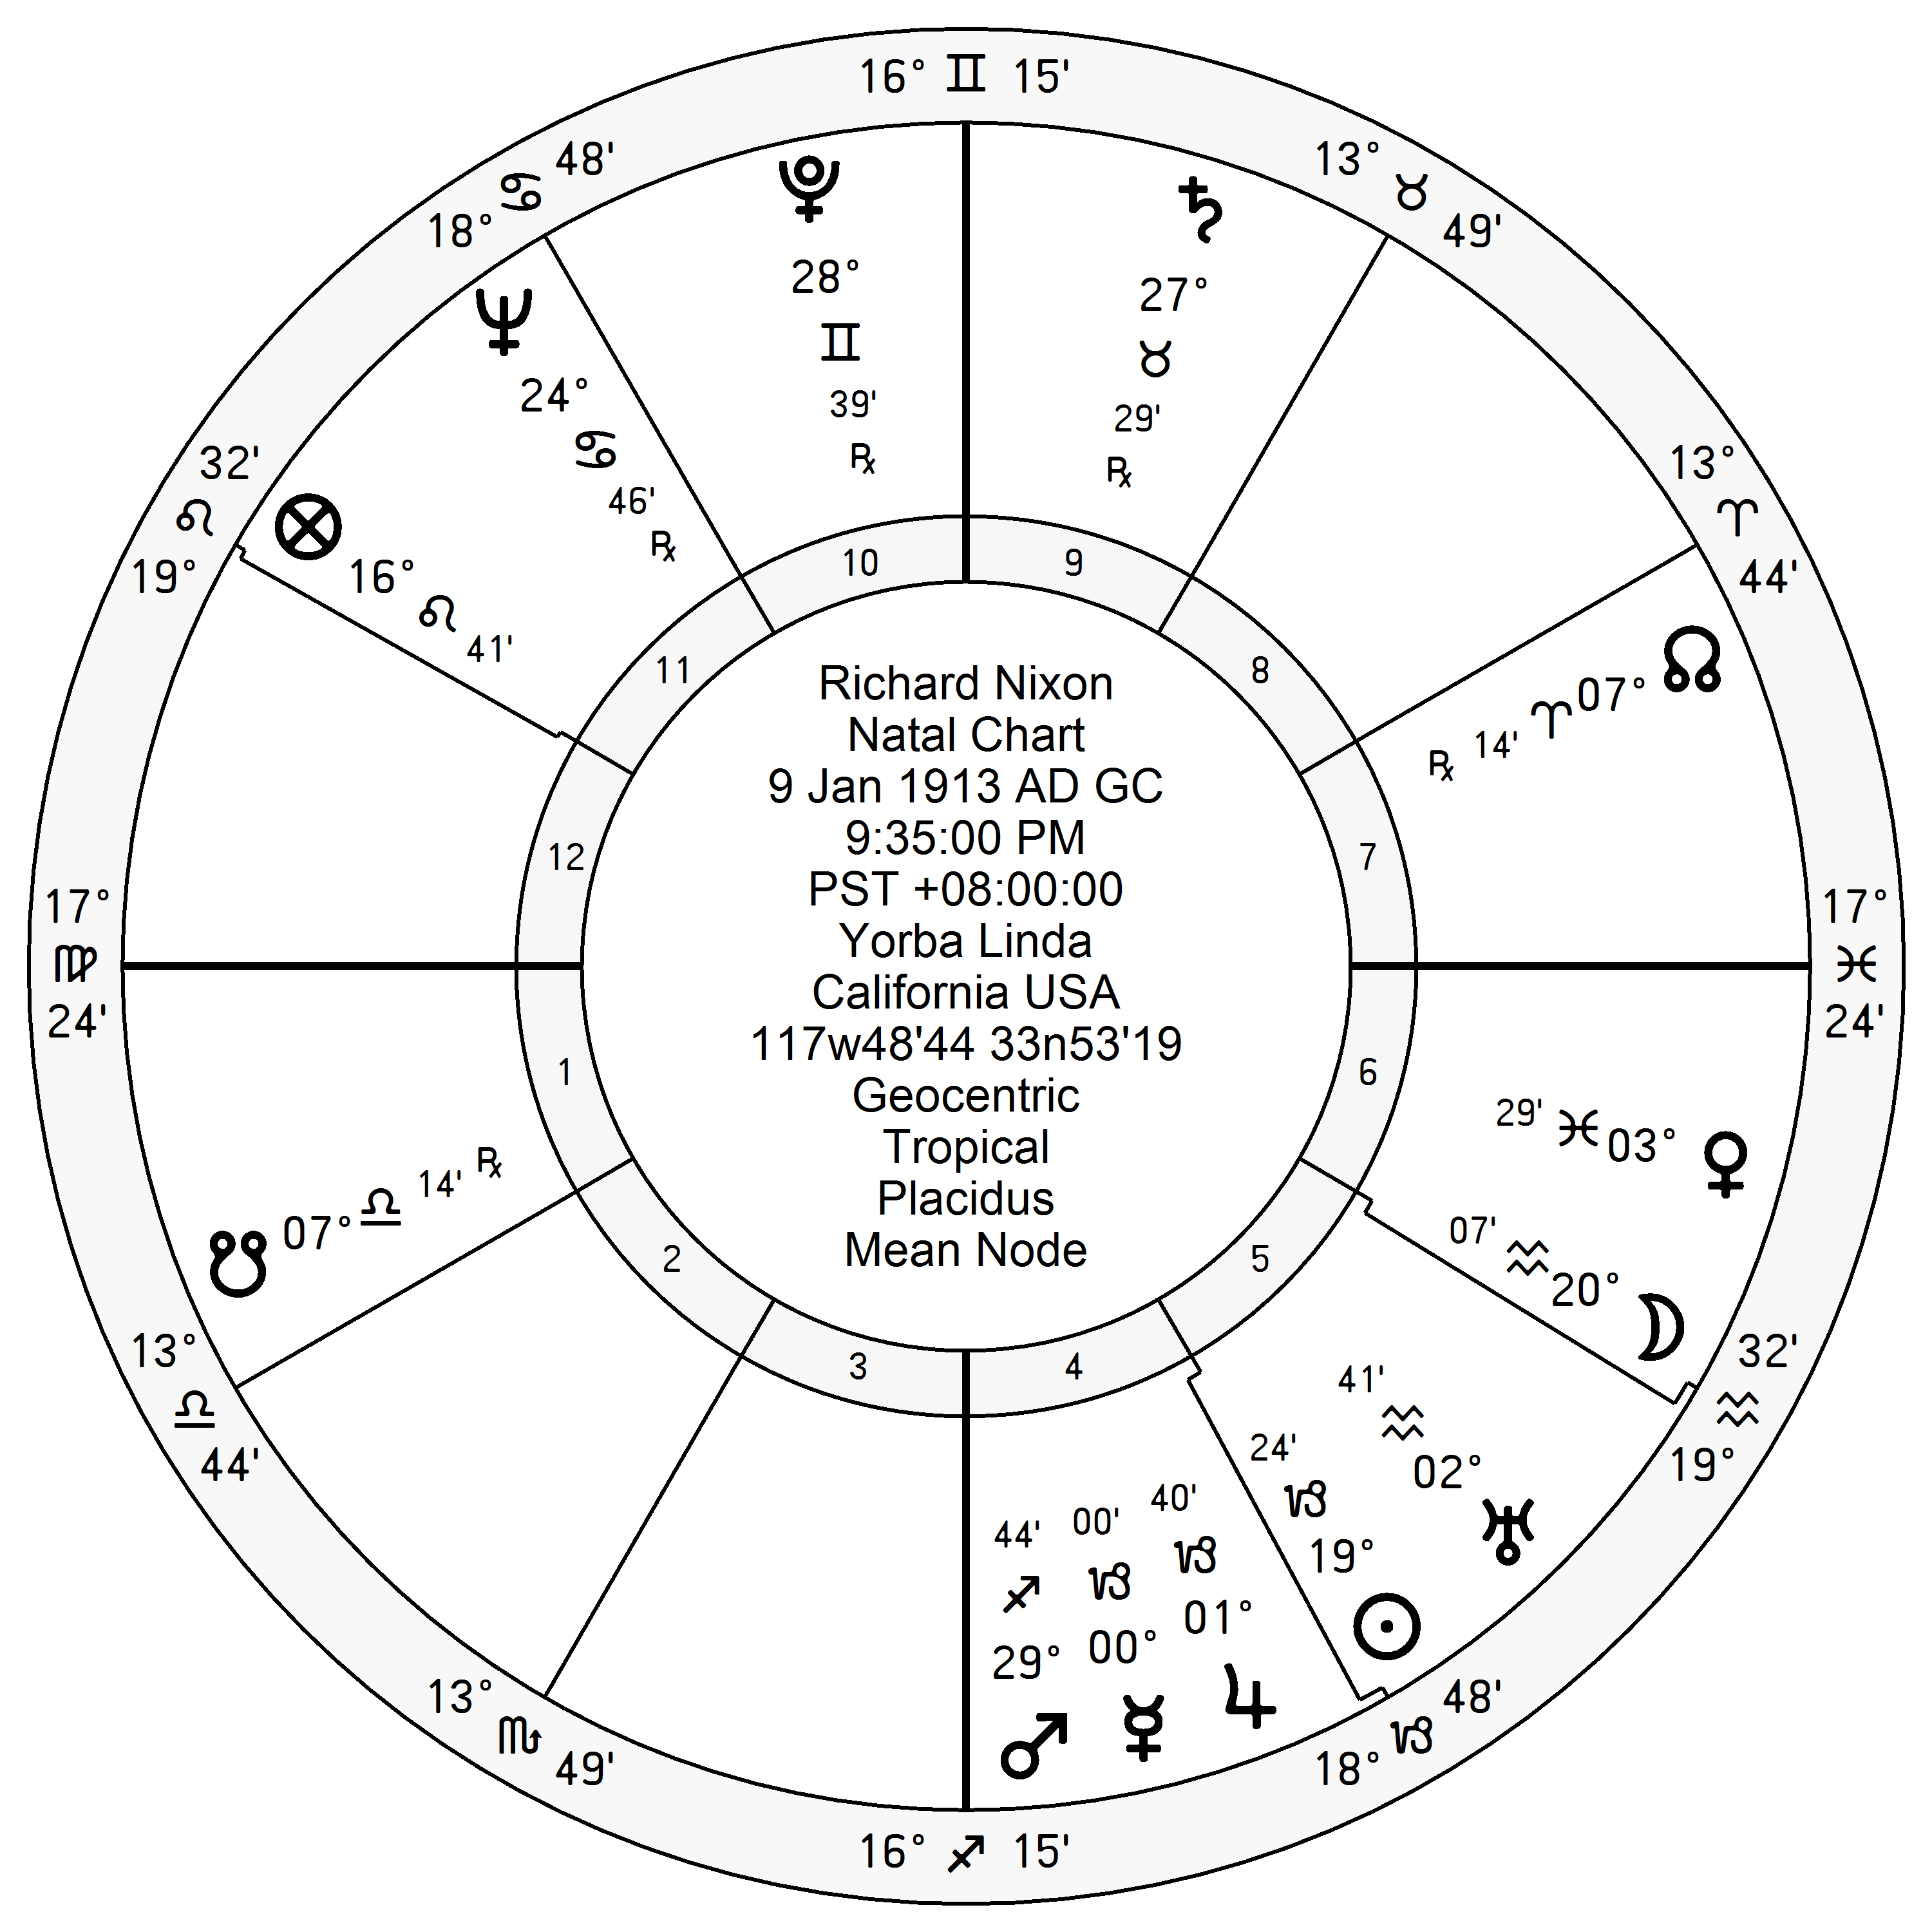
\includegraphics[width=0.9\textwidth]{charts/Nixon.png}}
\fontsize{8pt}{9pt}\selectfont

\Sun\, \Trine\, P10, \Trine\, N1 \\
\Venus\, \Square\, P10, \Opposition\, N1; \Trine\, N10 \\

The profection conditions are the same as those against JFK in 1960, only this time Nixon won.

\column{0.48\textwidth}
\vspace{-1em}
{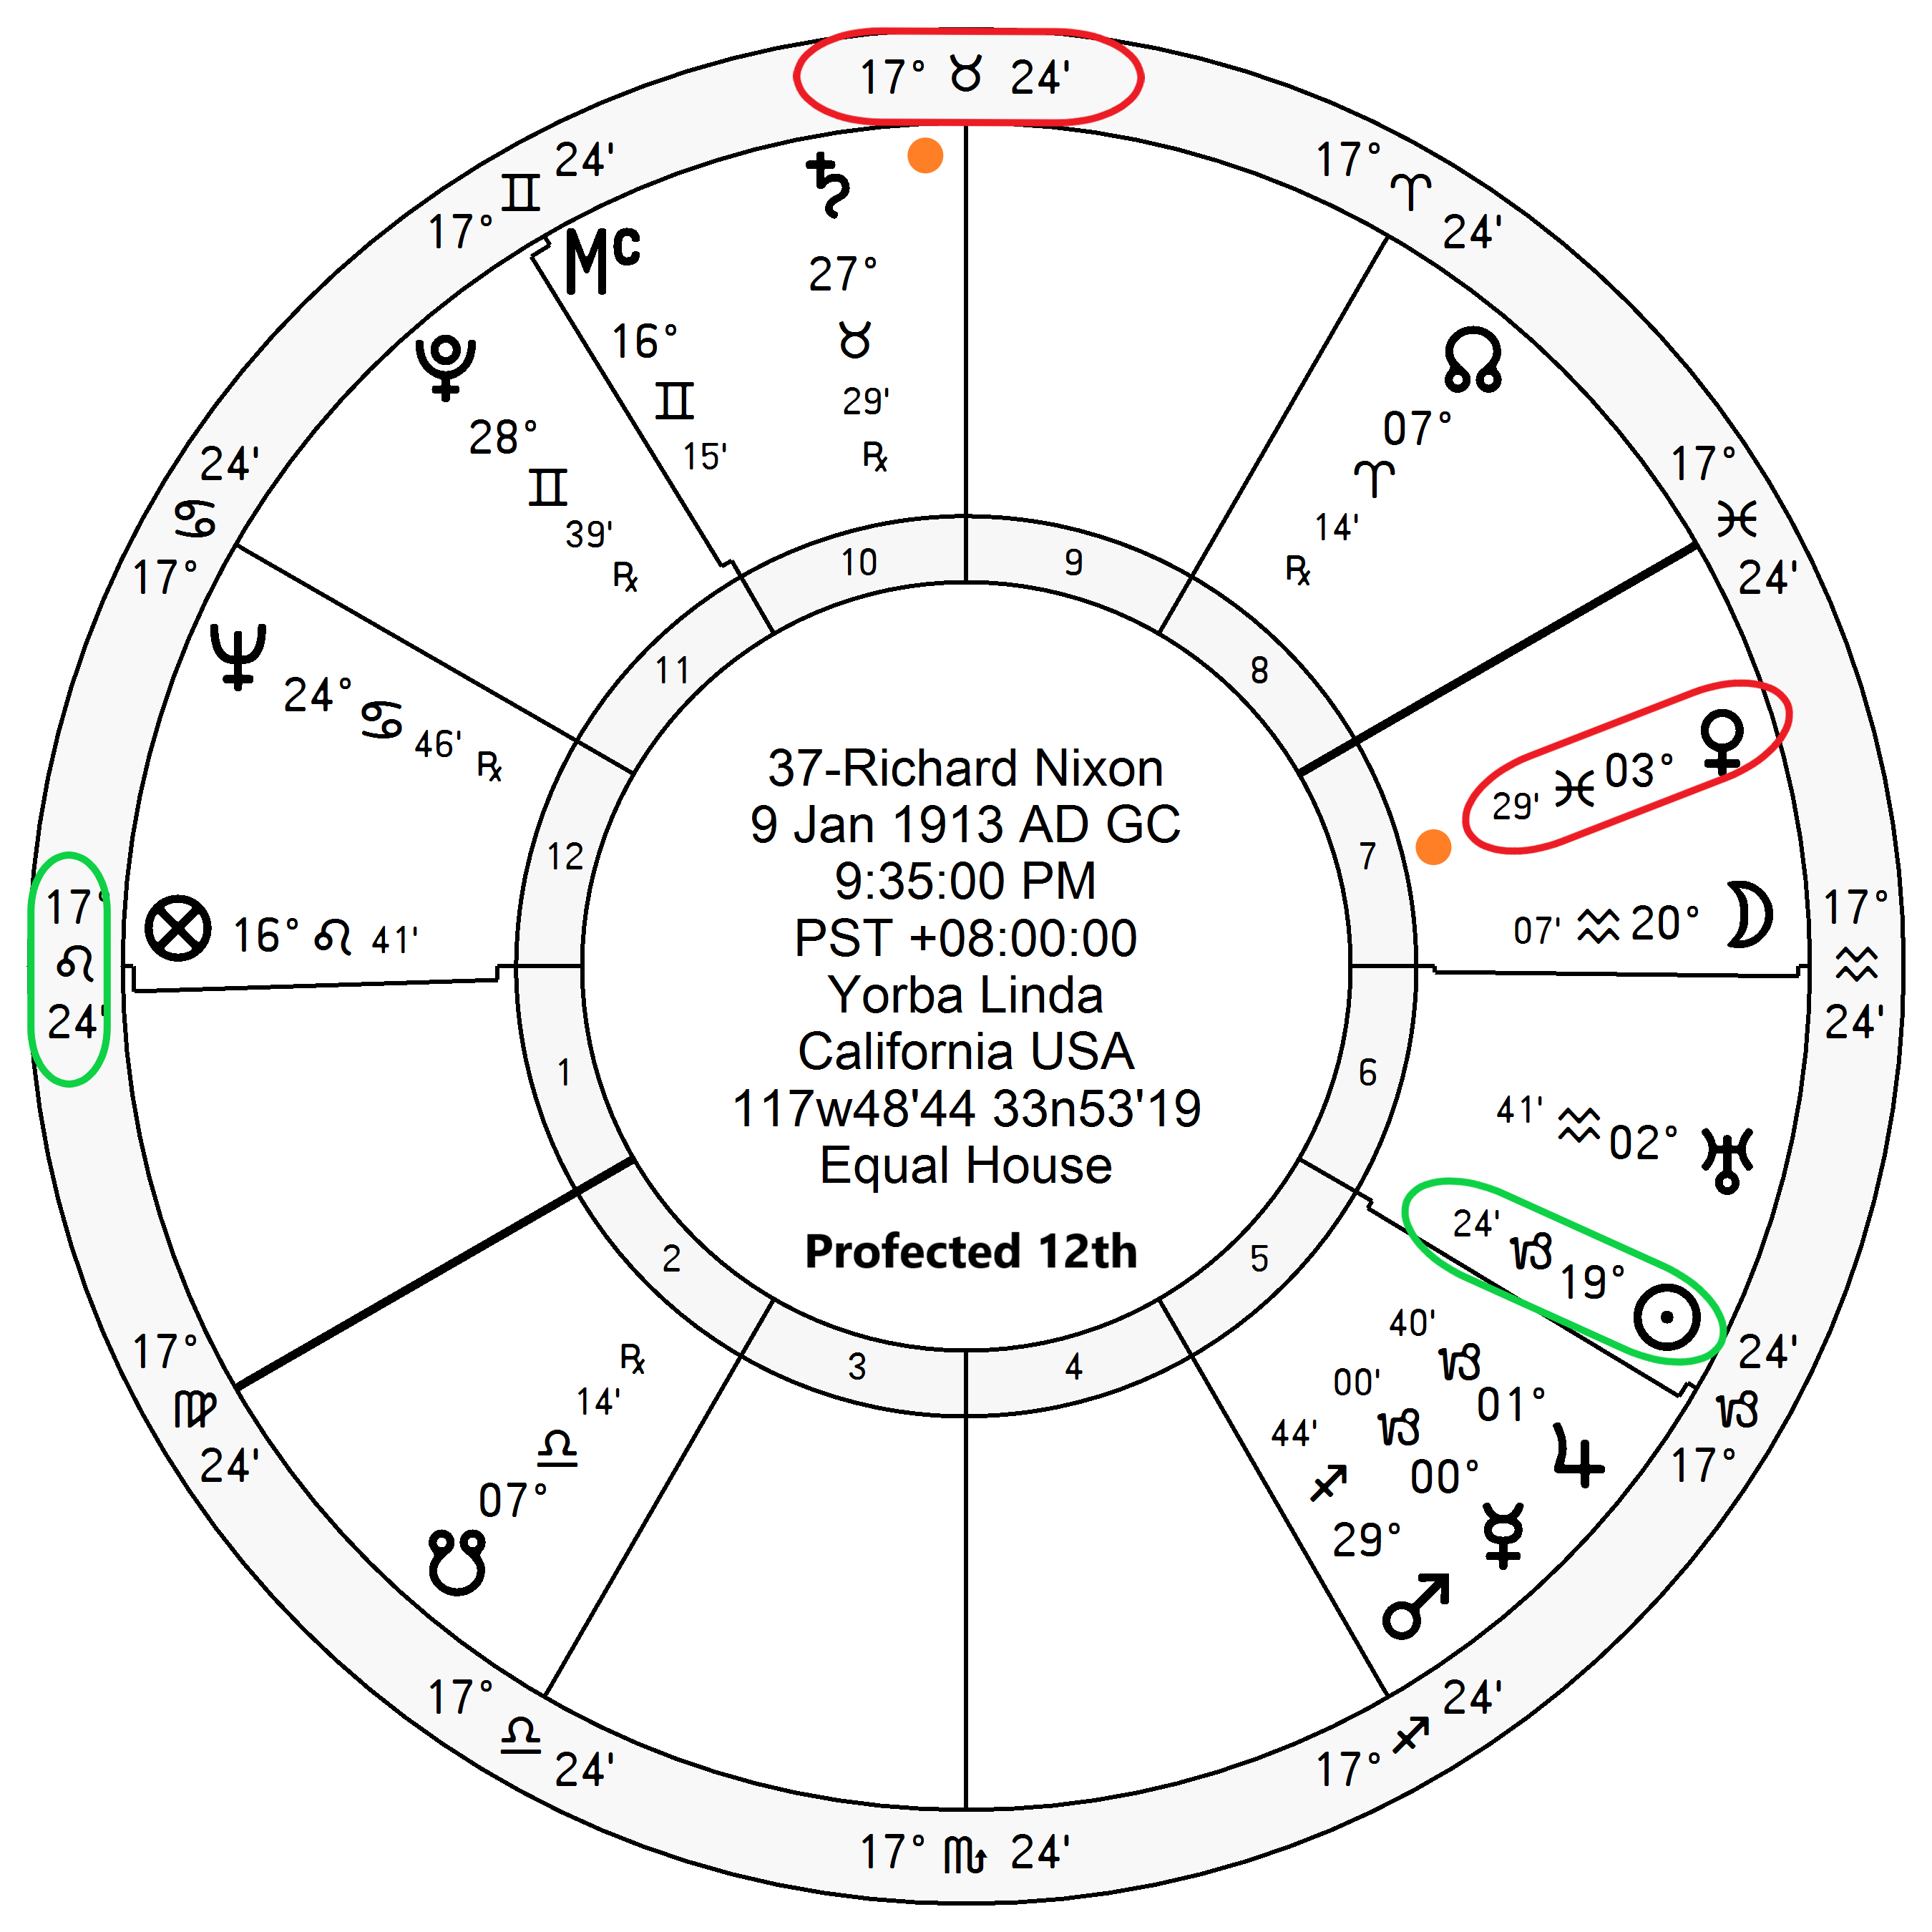
\includegraphics[width=0.9\textwidth]{charts/Nixon-Prof-12th.png}}
\fontsize{8pt}{9pt}\selectfont

\textbf{\dgreen P1=N12} 
	$\Rightarrow$ \Sun\, $\Rightarrow$ \textbf{\dgreen P6}/N5\\
\textbf{\red P10=N9}
	$\Rightarrow$ \Venus\, $\Rightarrow$ \textbf{\dgreen P7/N6}\\
PE=\textbf{\red P10/N9}
	 $\Rightarrow$ \Venus\, $\Rightarrow$ \textbf{\dgreen P7/N6}


\end{columns}
\end{frame}

% ===================================================
\begin{frame}[t]{Election November 7, 1972: George McGovern}
\small
\begin{columns}[T, onlytextwidth]
\column{0.48\textwidth}
\vspace{-1em}
{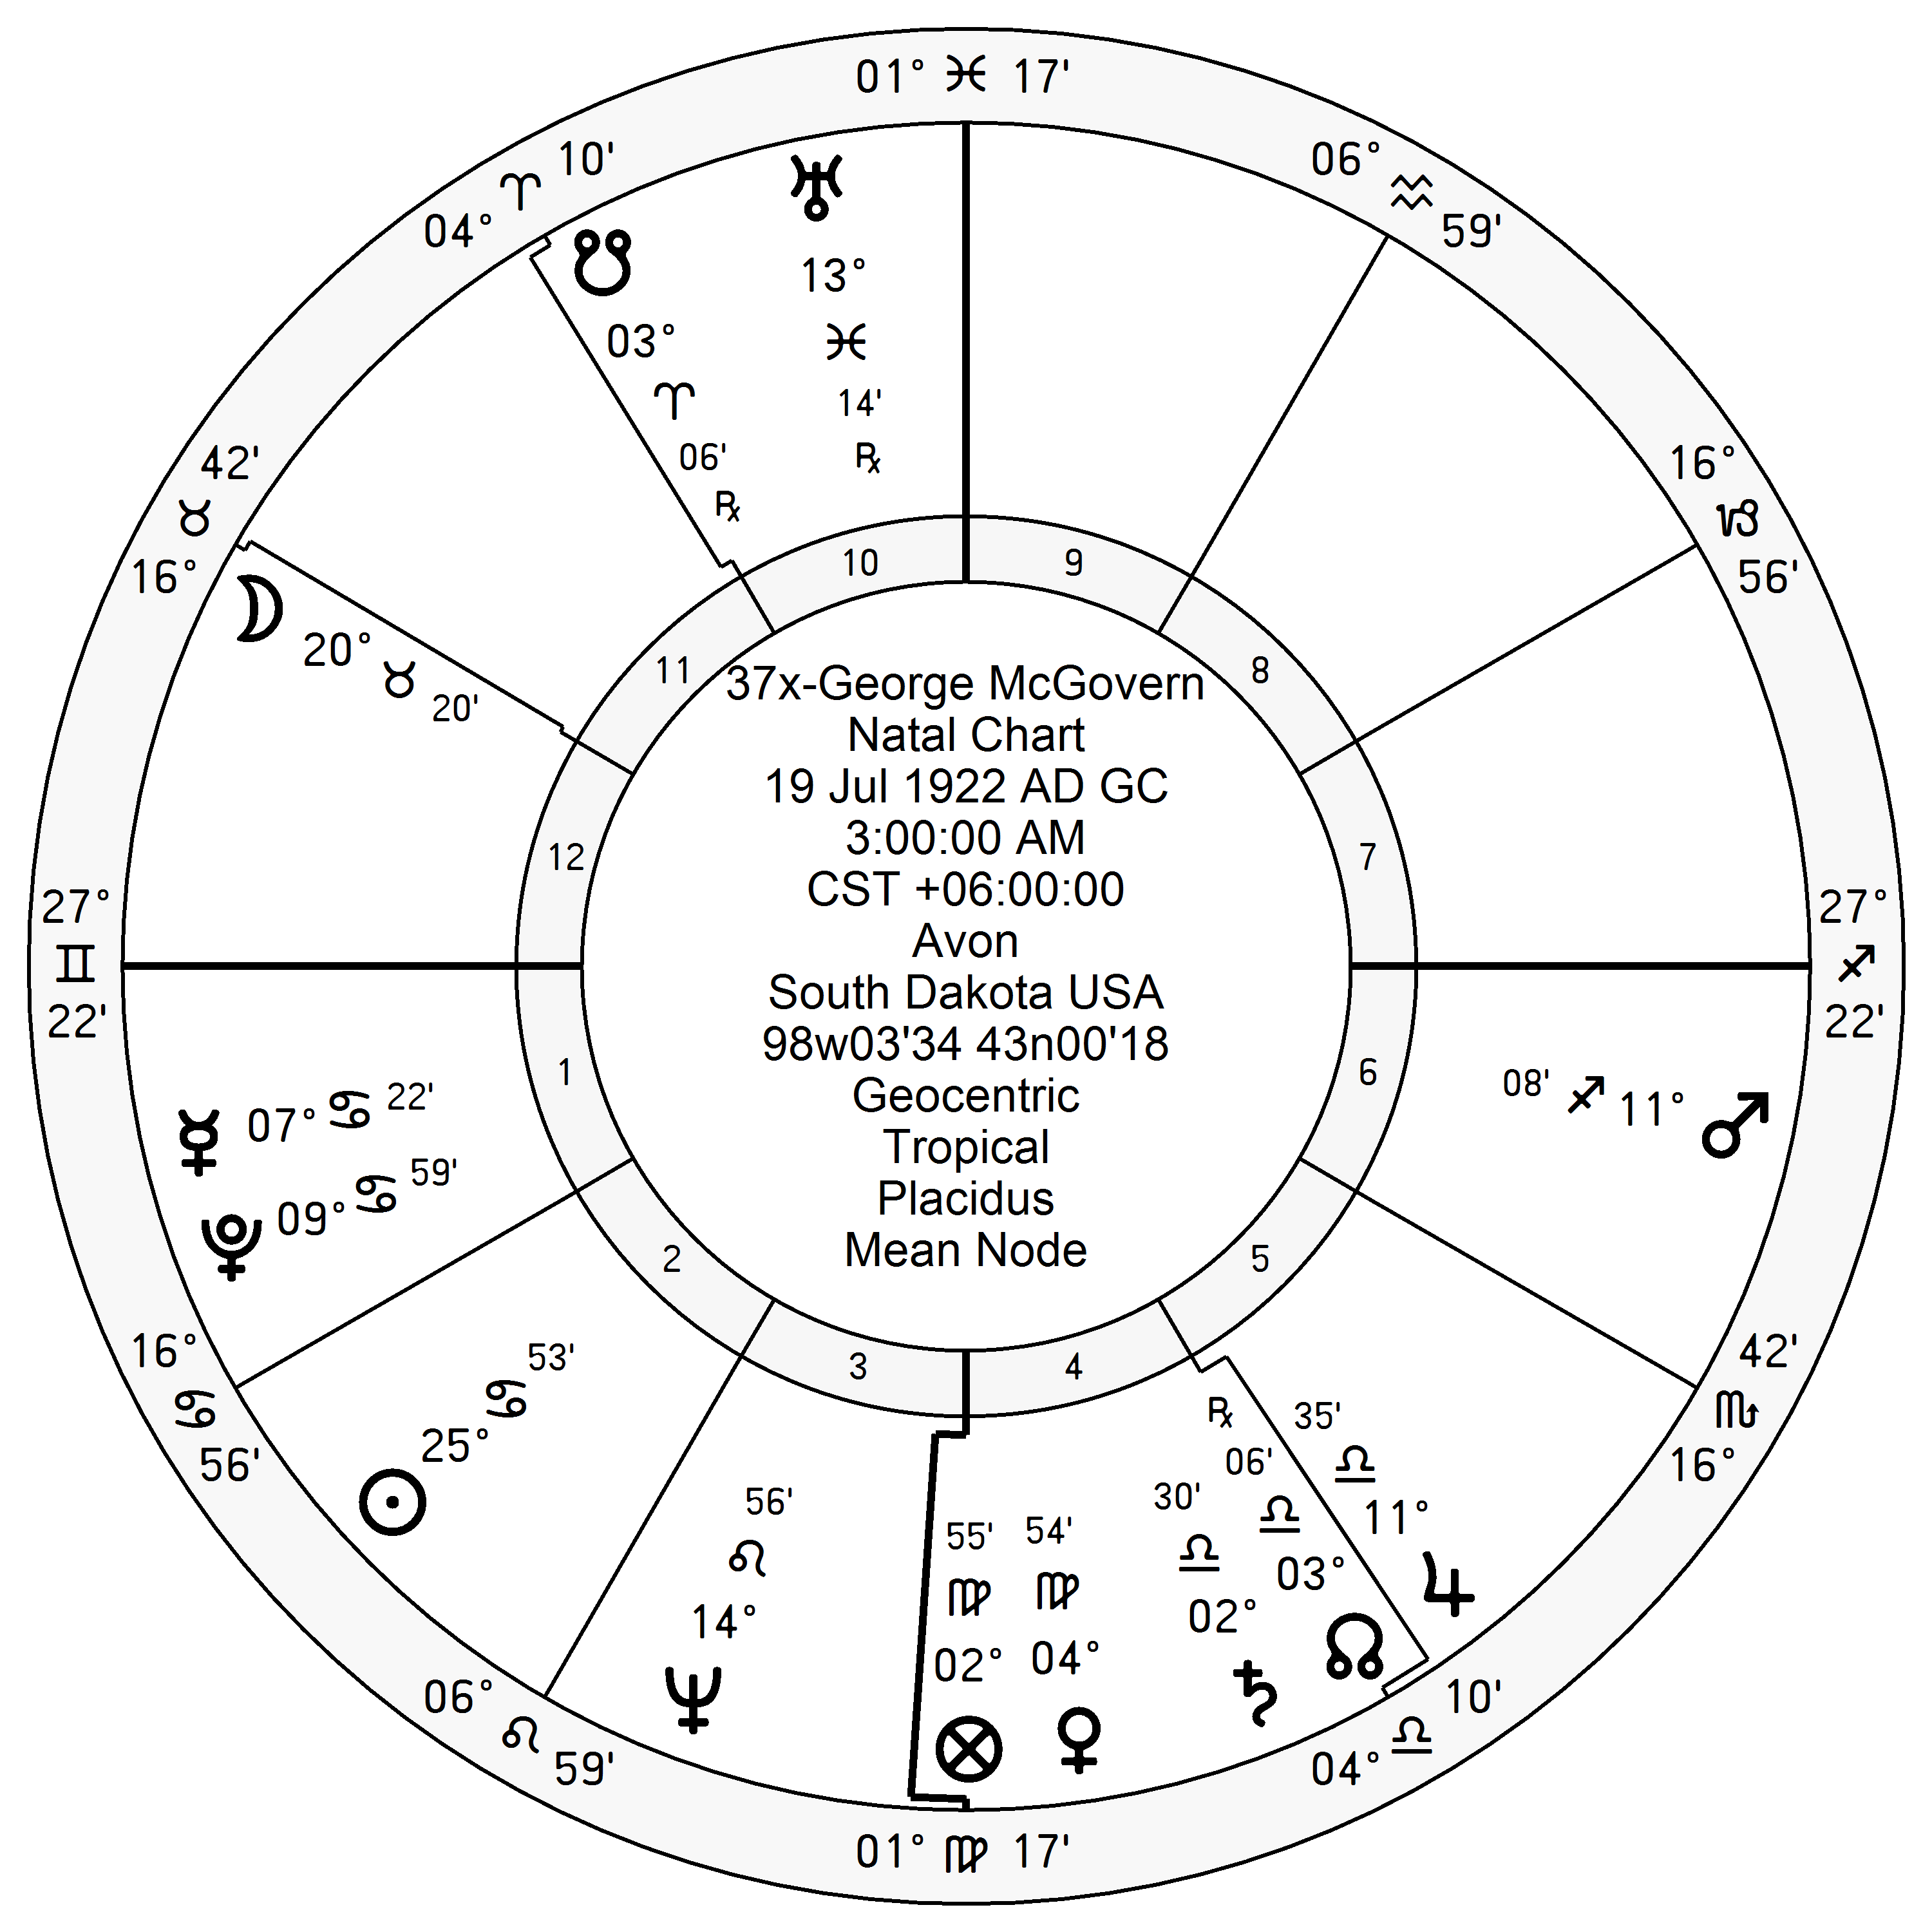
\includegraphics[width=0.9\textwidth]{charts/McGovern.png}}
\fontsize{8pt}{9pt}\selectfont

\Sun\, \Trine\, N10 \\
\Venus\, in P1, \Sextile\, N1; \Square\, P10, \Opposition\, N10 \\
\Mars\, \Opposition\, P10, \Square\, P1; \Square\, N10 \\
\vspace{0.5em}
The chart looks stronger than Nixon; \SouthNode\, in N10 weakens 10th? \Mars\, \Square\, \Venus?

\column{0.48\textwidth}
\vspace{-1em}
{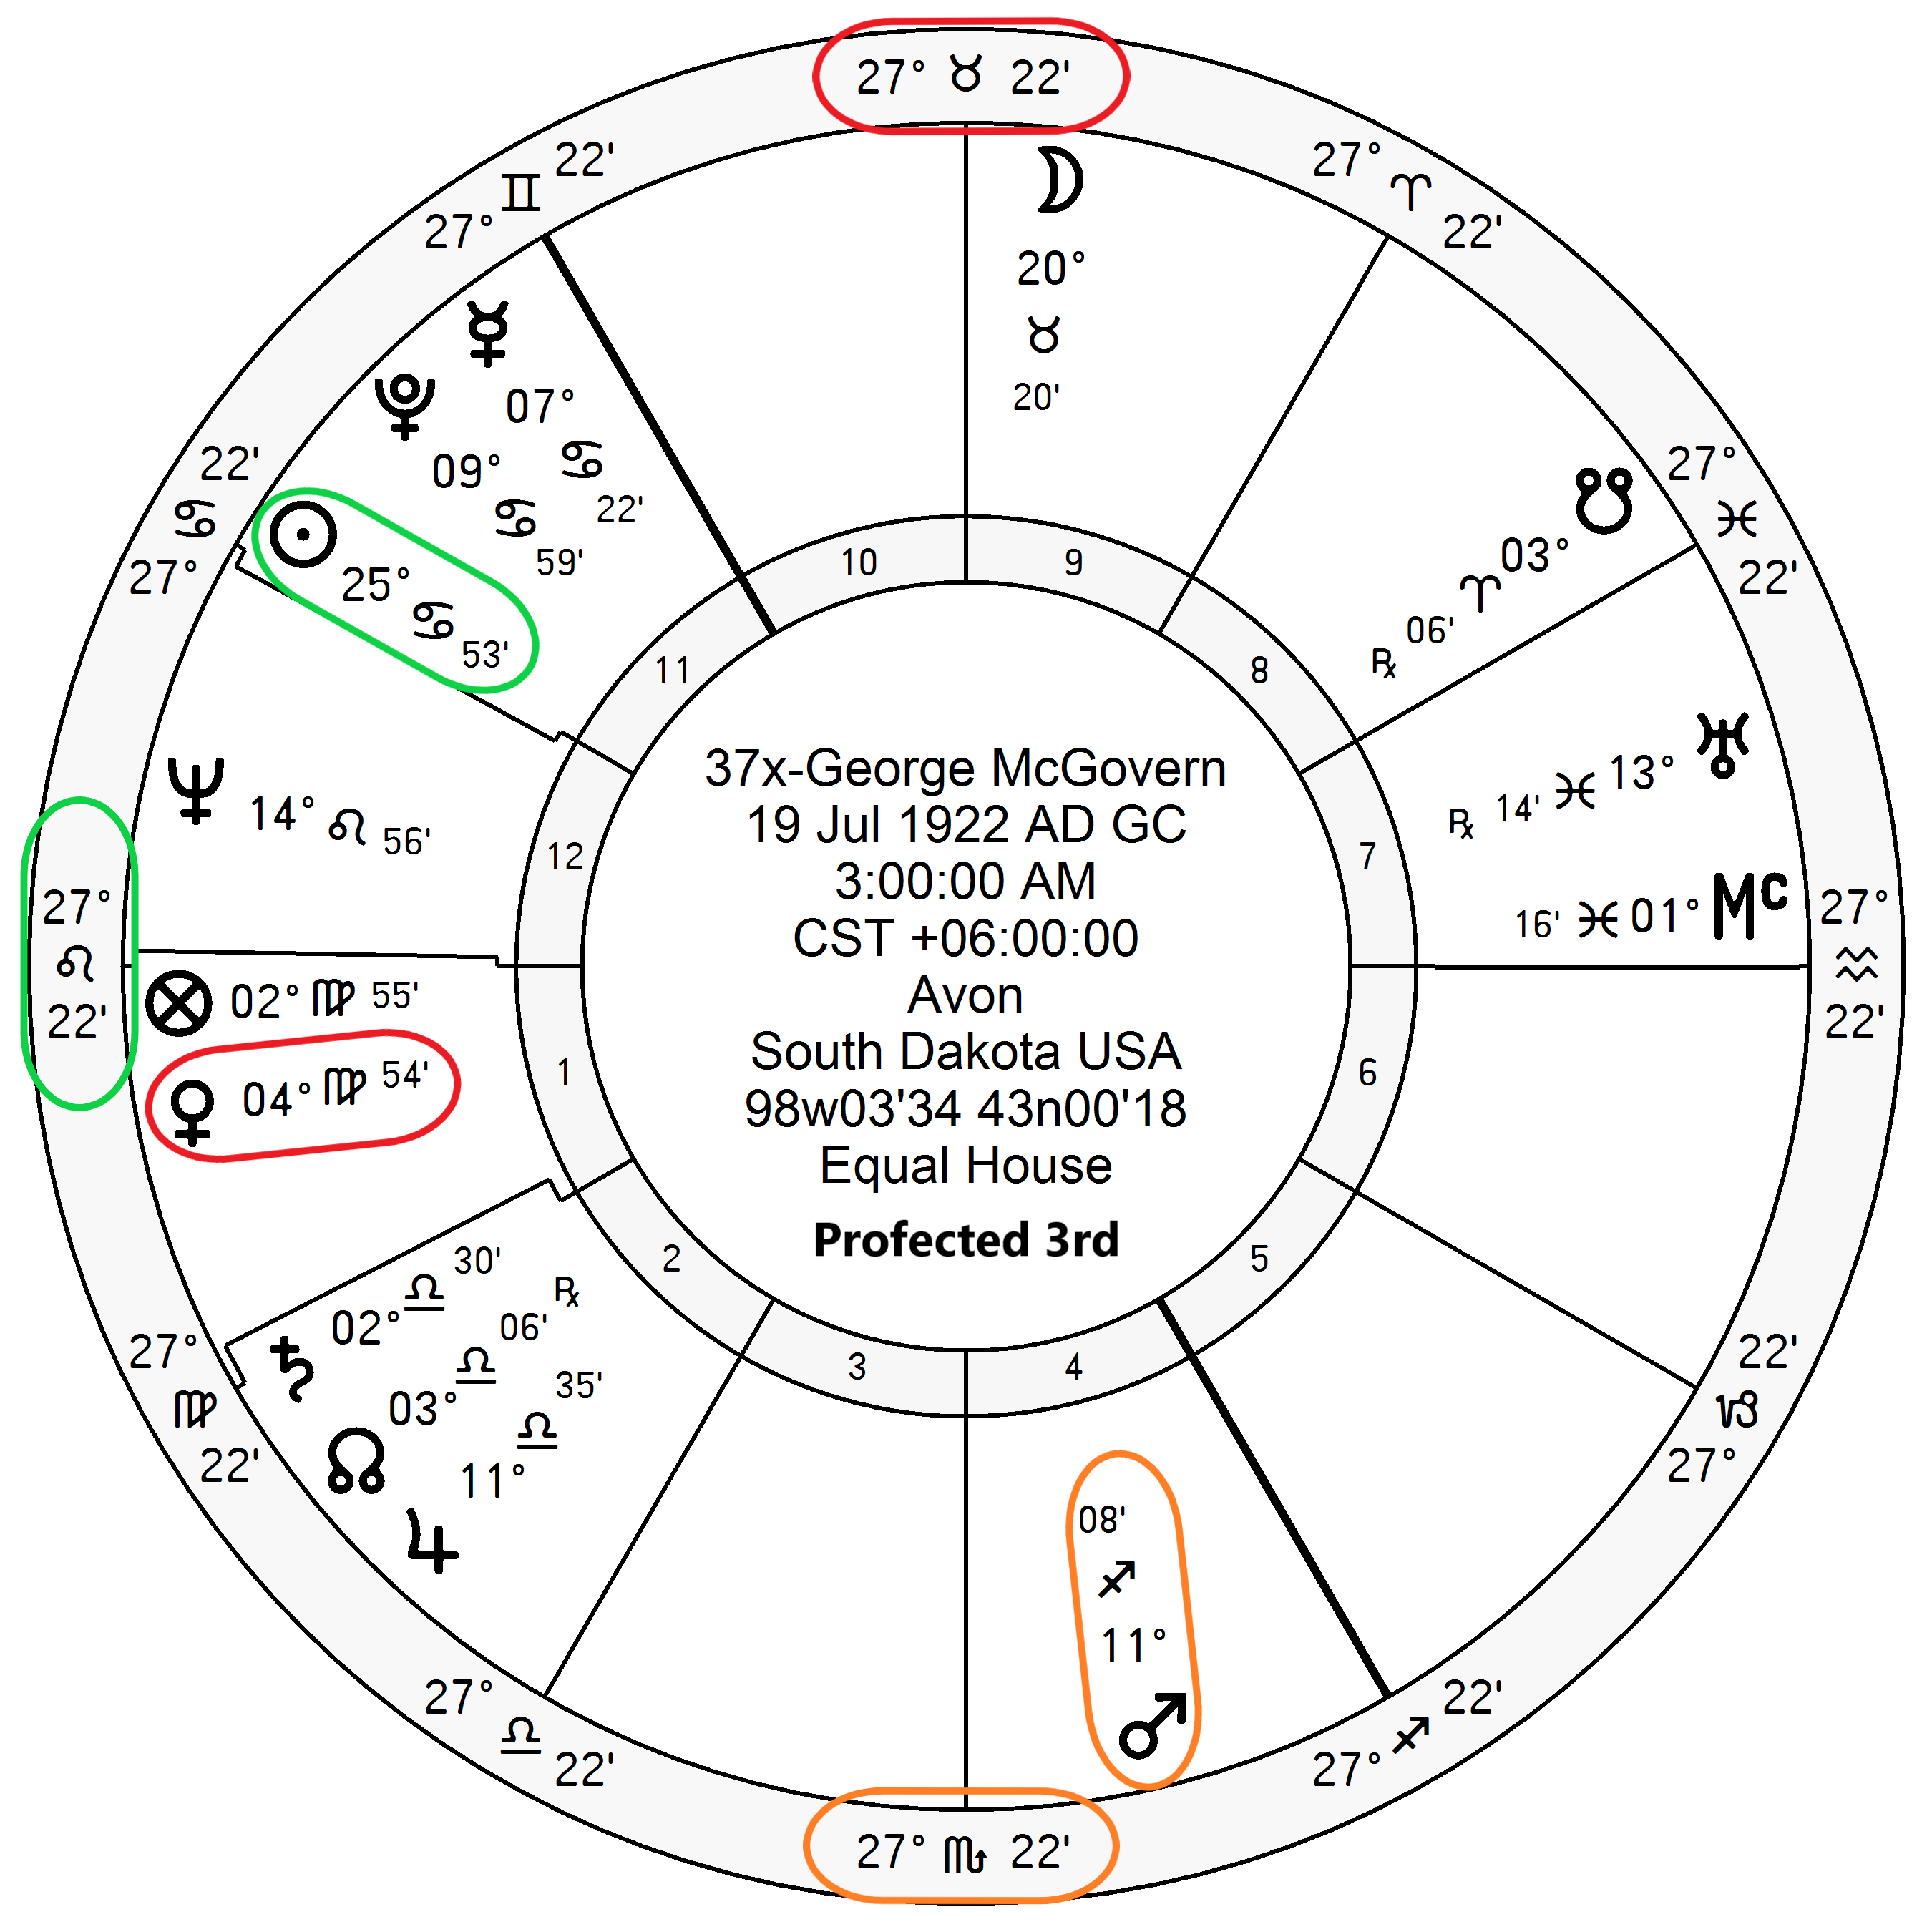
\includegraphics[width=0.9\textwidth]{charts/McGovern-Prof-3rd.png}}
\fontsize{8pt}{9pt}\selectfont
\textbf{\dgreen P1}=N3
	$\Rightarrow$ \Sun\, $\Rightarrow$ P11/N2\\
\textbf{\red P10=N12}
	$\Rightarrow$ \Venus\, $\Rightarrow$ \textbf{\dgreen P1}/\textbf{\red N4}\\
PE=\textbf{\red P4/N6}
	 $\Rightarrow$ \Mars\, $\Rightarrow$ \textbf{\red P4/N6}

\end{columns}
\end{frame}

%\subsection{Election November 2, 1976: *Carter vs Ford}
\begin{frame}[t]{Election November 2, 1976: *Jimmy Carter}
\small

\begin{columns}[T, onlytextwidth]
\column{0.48\textwidth}
\vspace{-1em}
{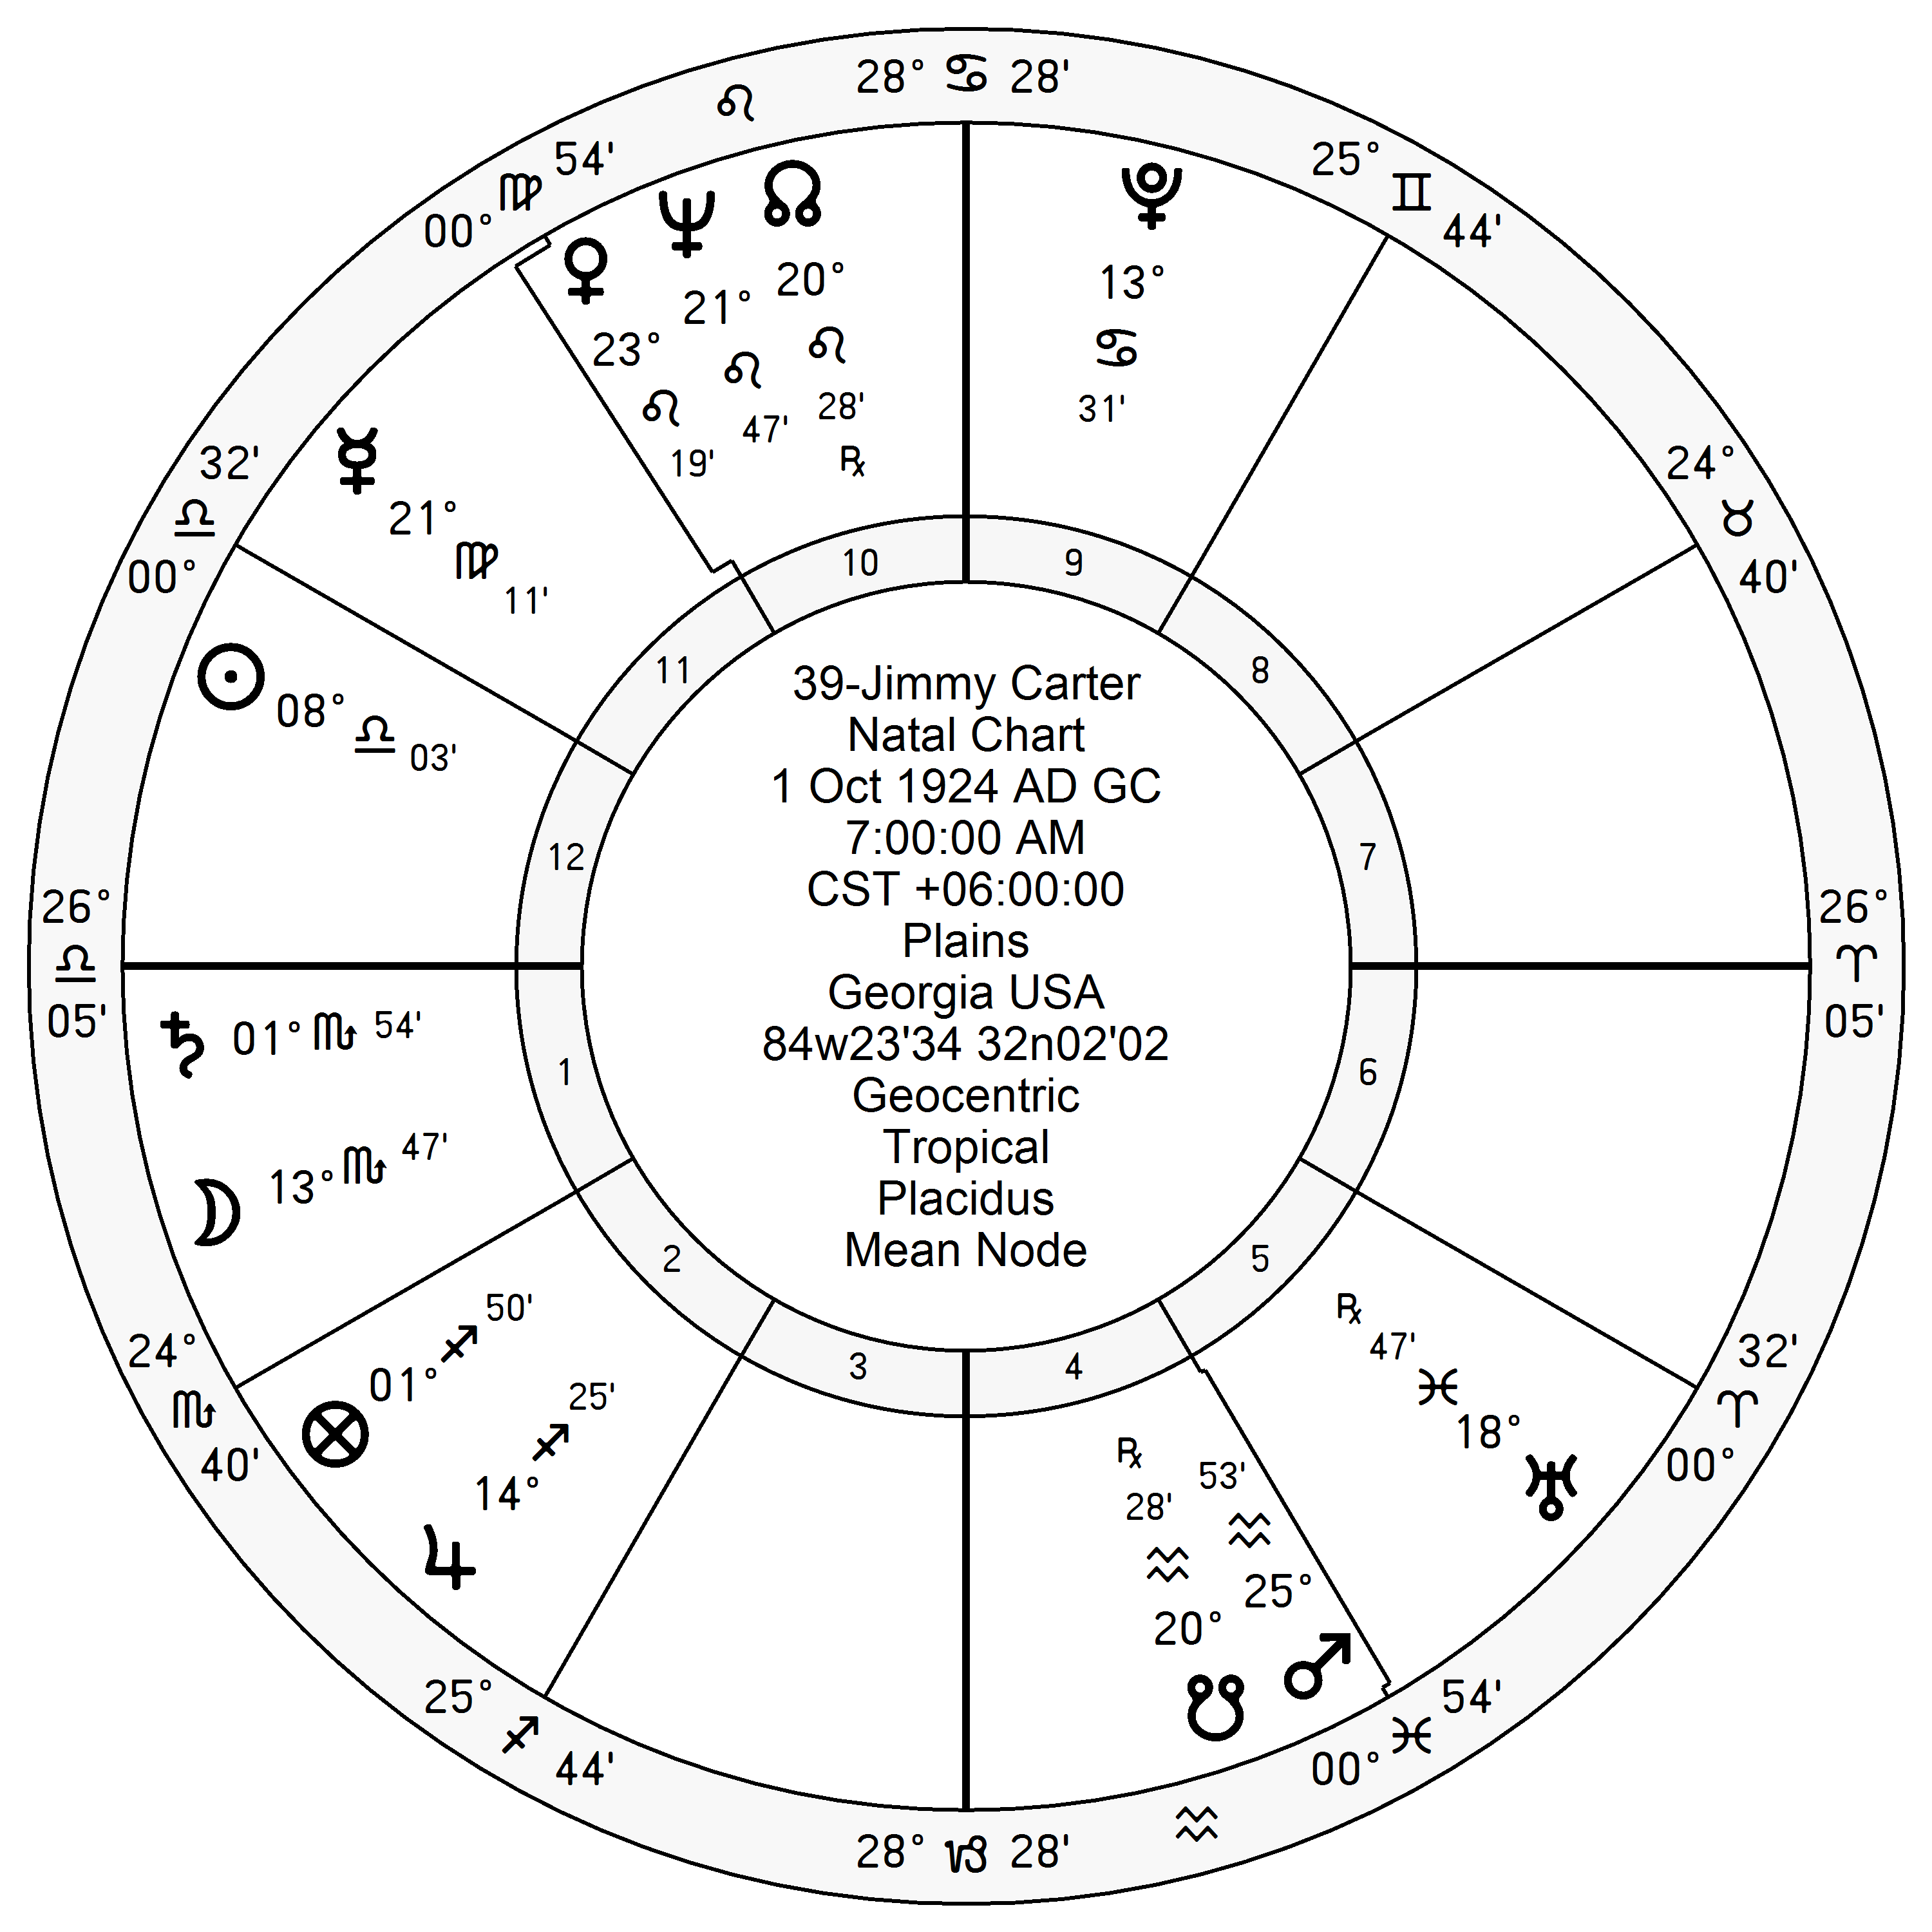
\includegraphics[width=0.9\textwidth]{charts/Carter.png}}

\Saturn\, \Trine\, P1; in N1, \Sextile\, N10 \\
\Mars\, \Sextile\, P10 \\
\Jupiter\, in domicile in P10, \Square\, P1; \Trine\, N10

\column{0.48\textwidth}
\vspace{-1em}
{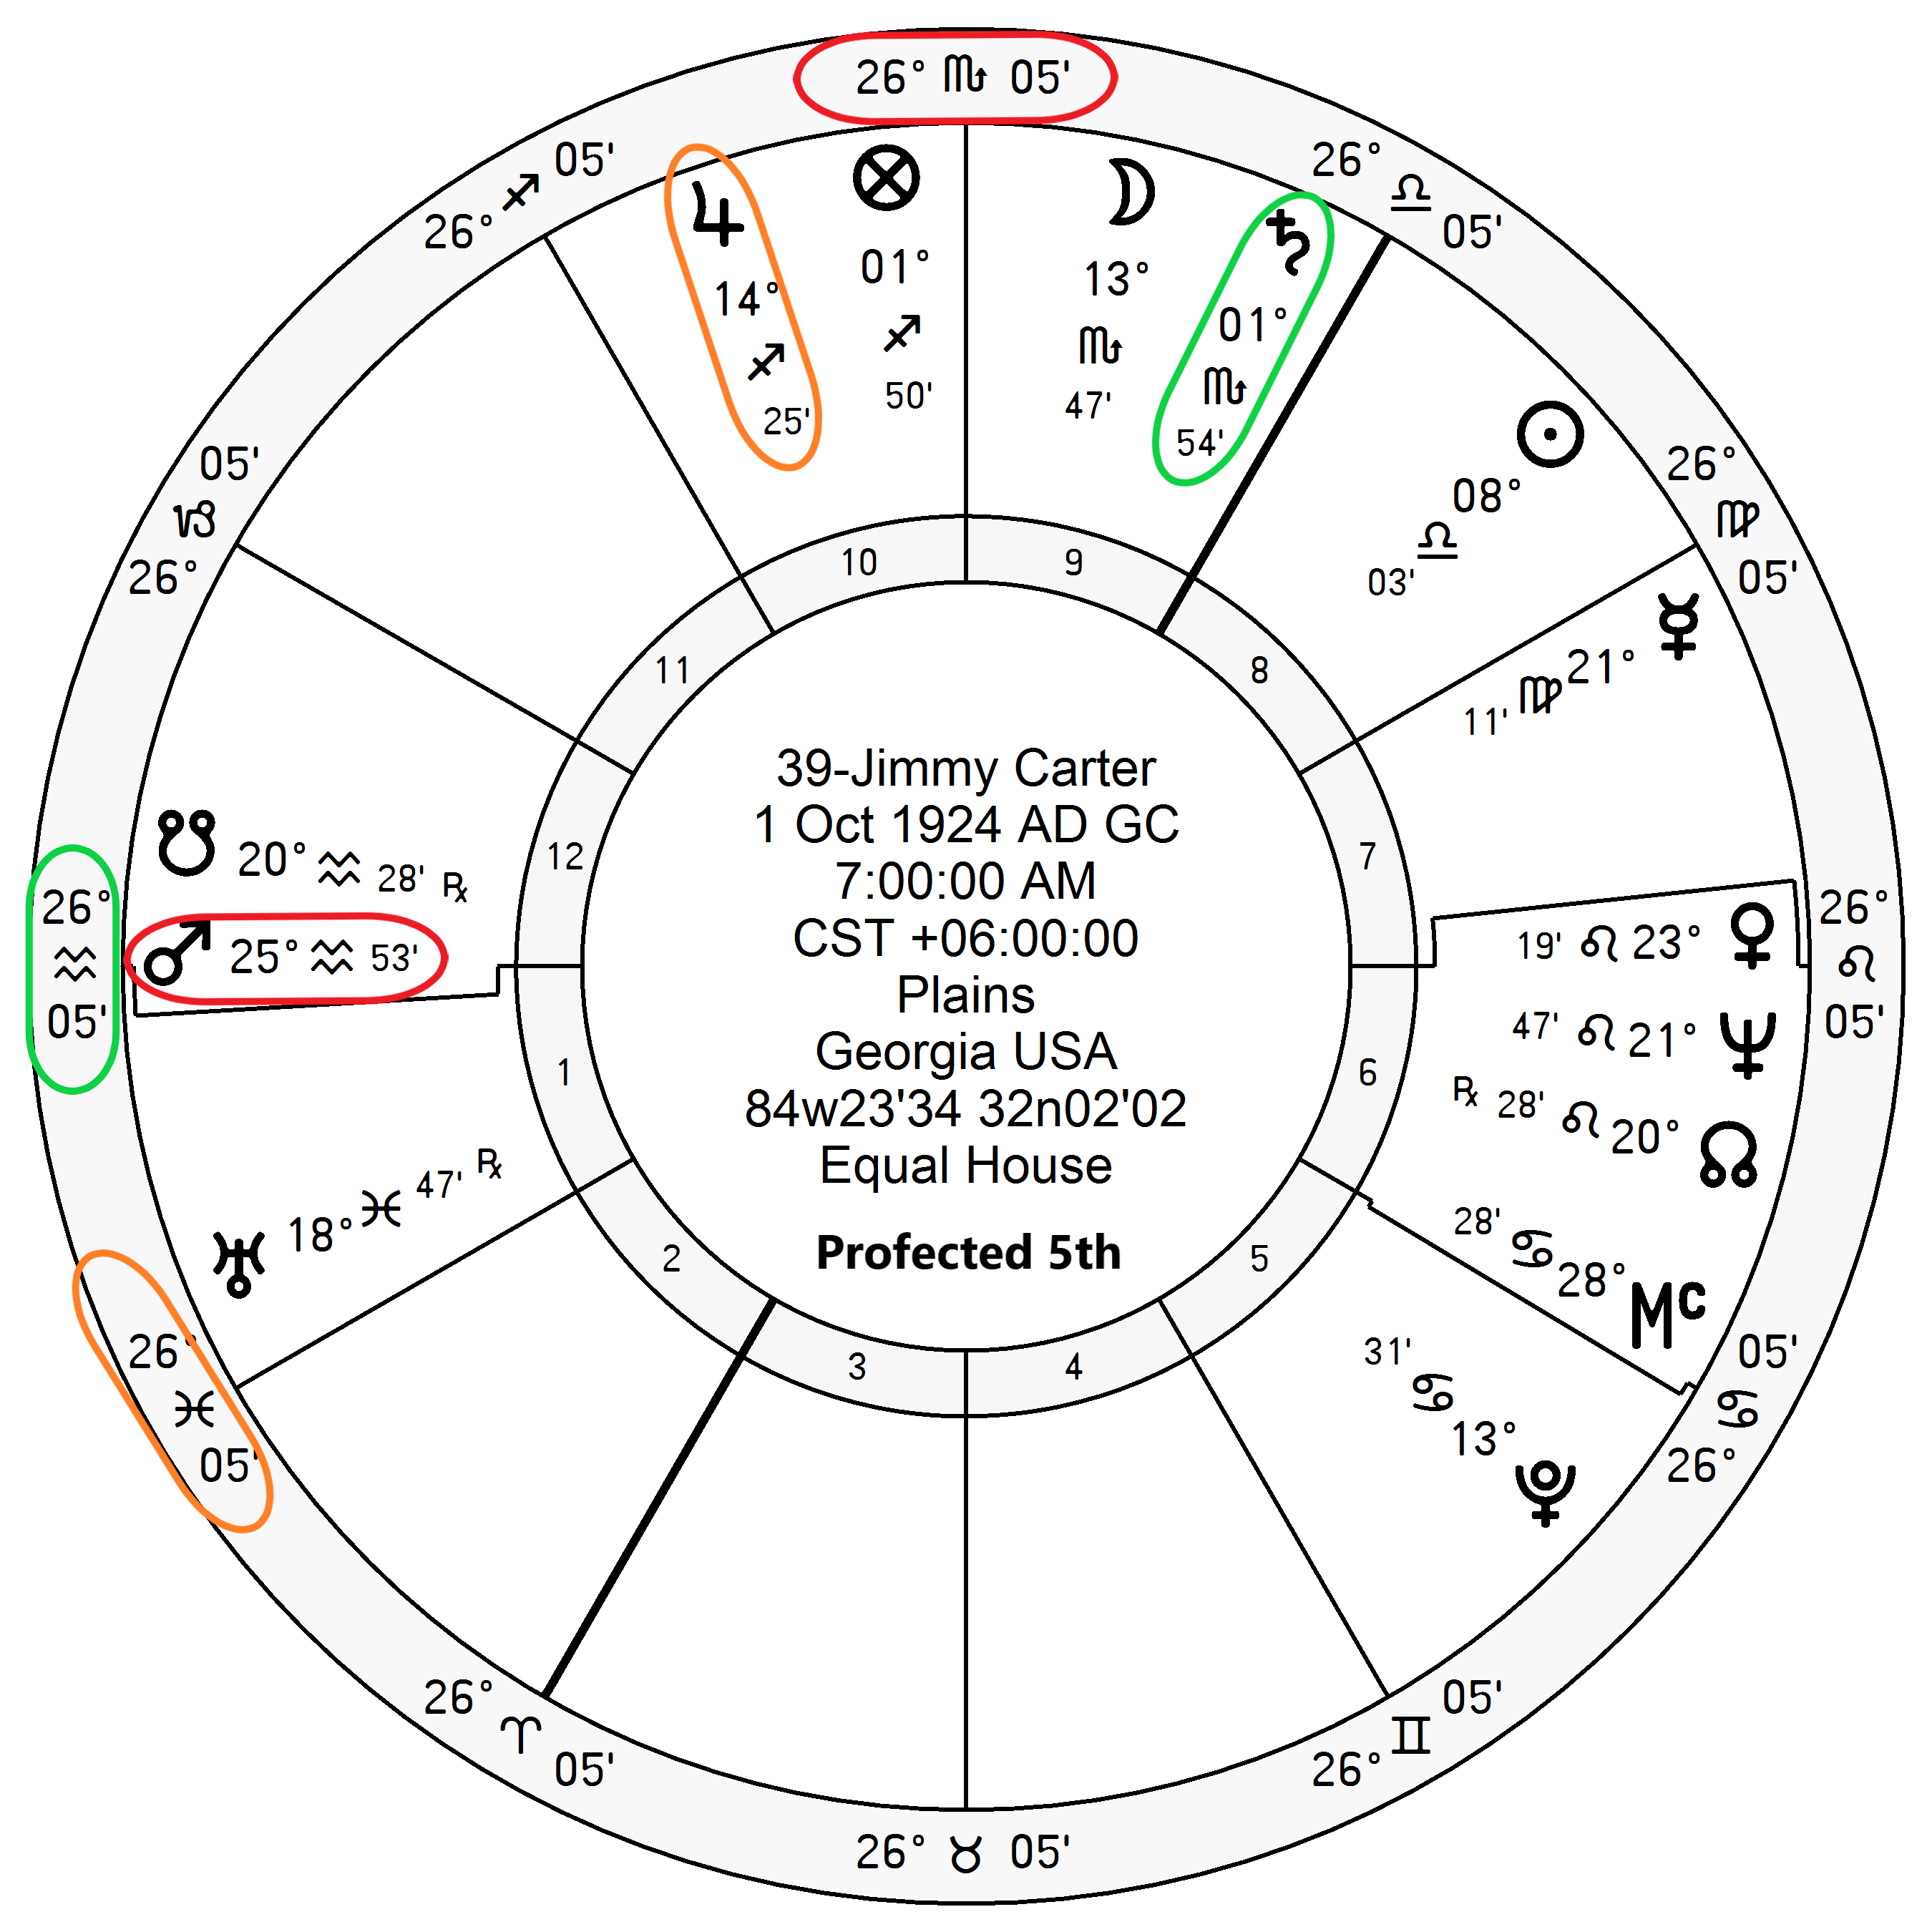
\includegraphics[width=0.9\textwidth]{charts/Carter-Prof-5th.png}}
\fontsize{8pt}{9pt}\selectfont

\textbf{\dgreen P1=N4} 
	$\Rightarrow$ \Saturn\, $\Rightarrow$ P9/\textbf{\dgreen N1}\\
\textbf{\red P10=N2}
	$\Rightarrow$ \Mars\, $\Rightarrow$ P12/\textbf{\dgreen N4}\\
PE=\textbf{\red P2}/N5
	 $\Rightarrow$ \Jupiter\, $\Rightarrow$ \textbf{\red P10/N2}


\end{columns}
\end{frame}

% ===================================================
\begin{frame}[t]{Election November 2, 1976: Gerald Ford}
\small
\begin{columns}[T, onlytextwidth]
\column{0.48\textwidth}
\vspace{-1em}
{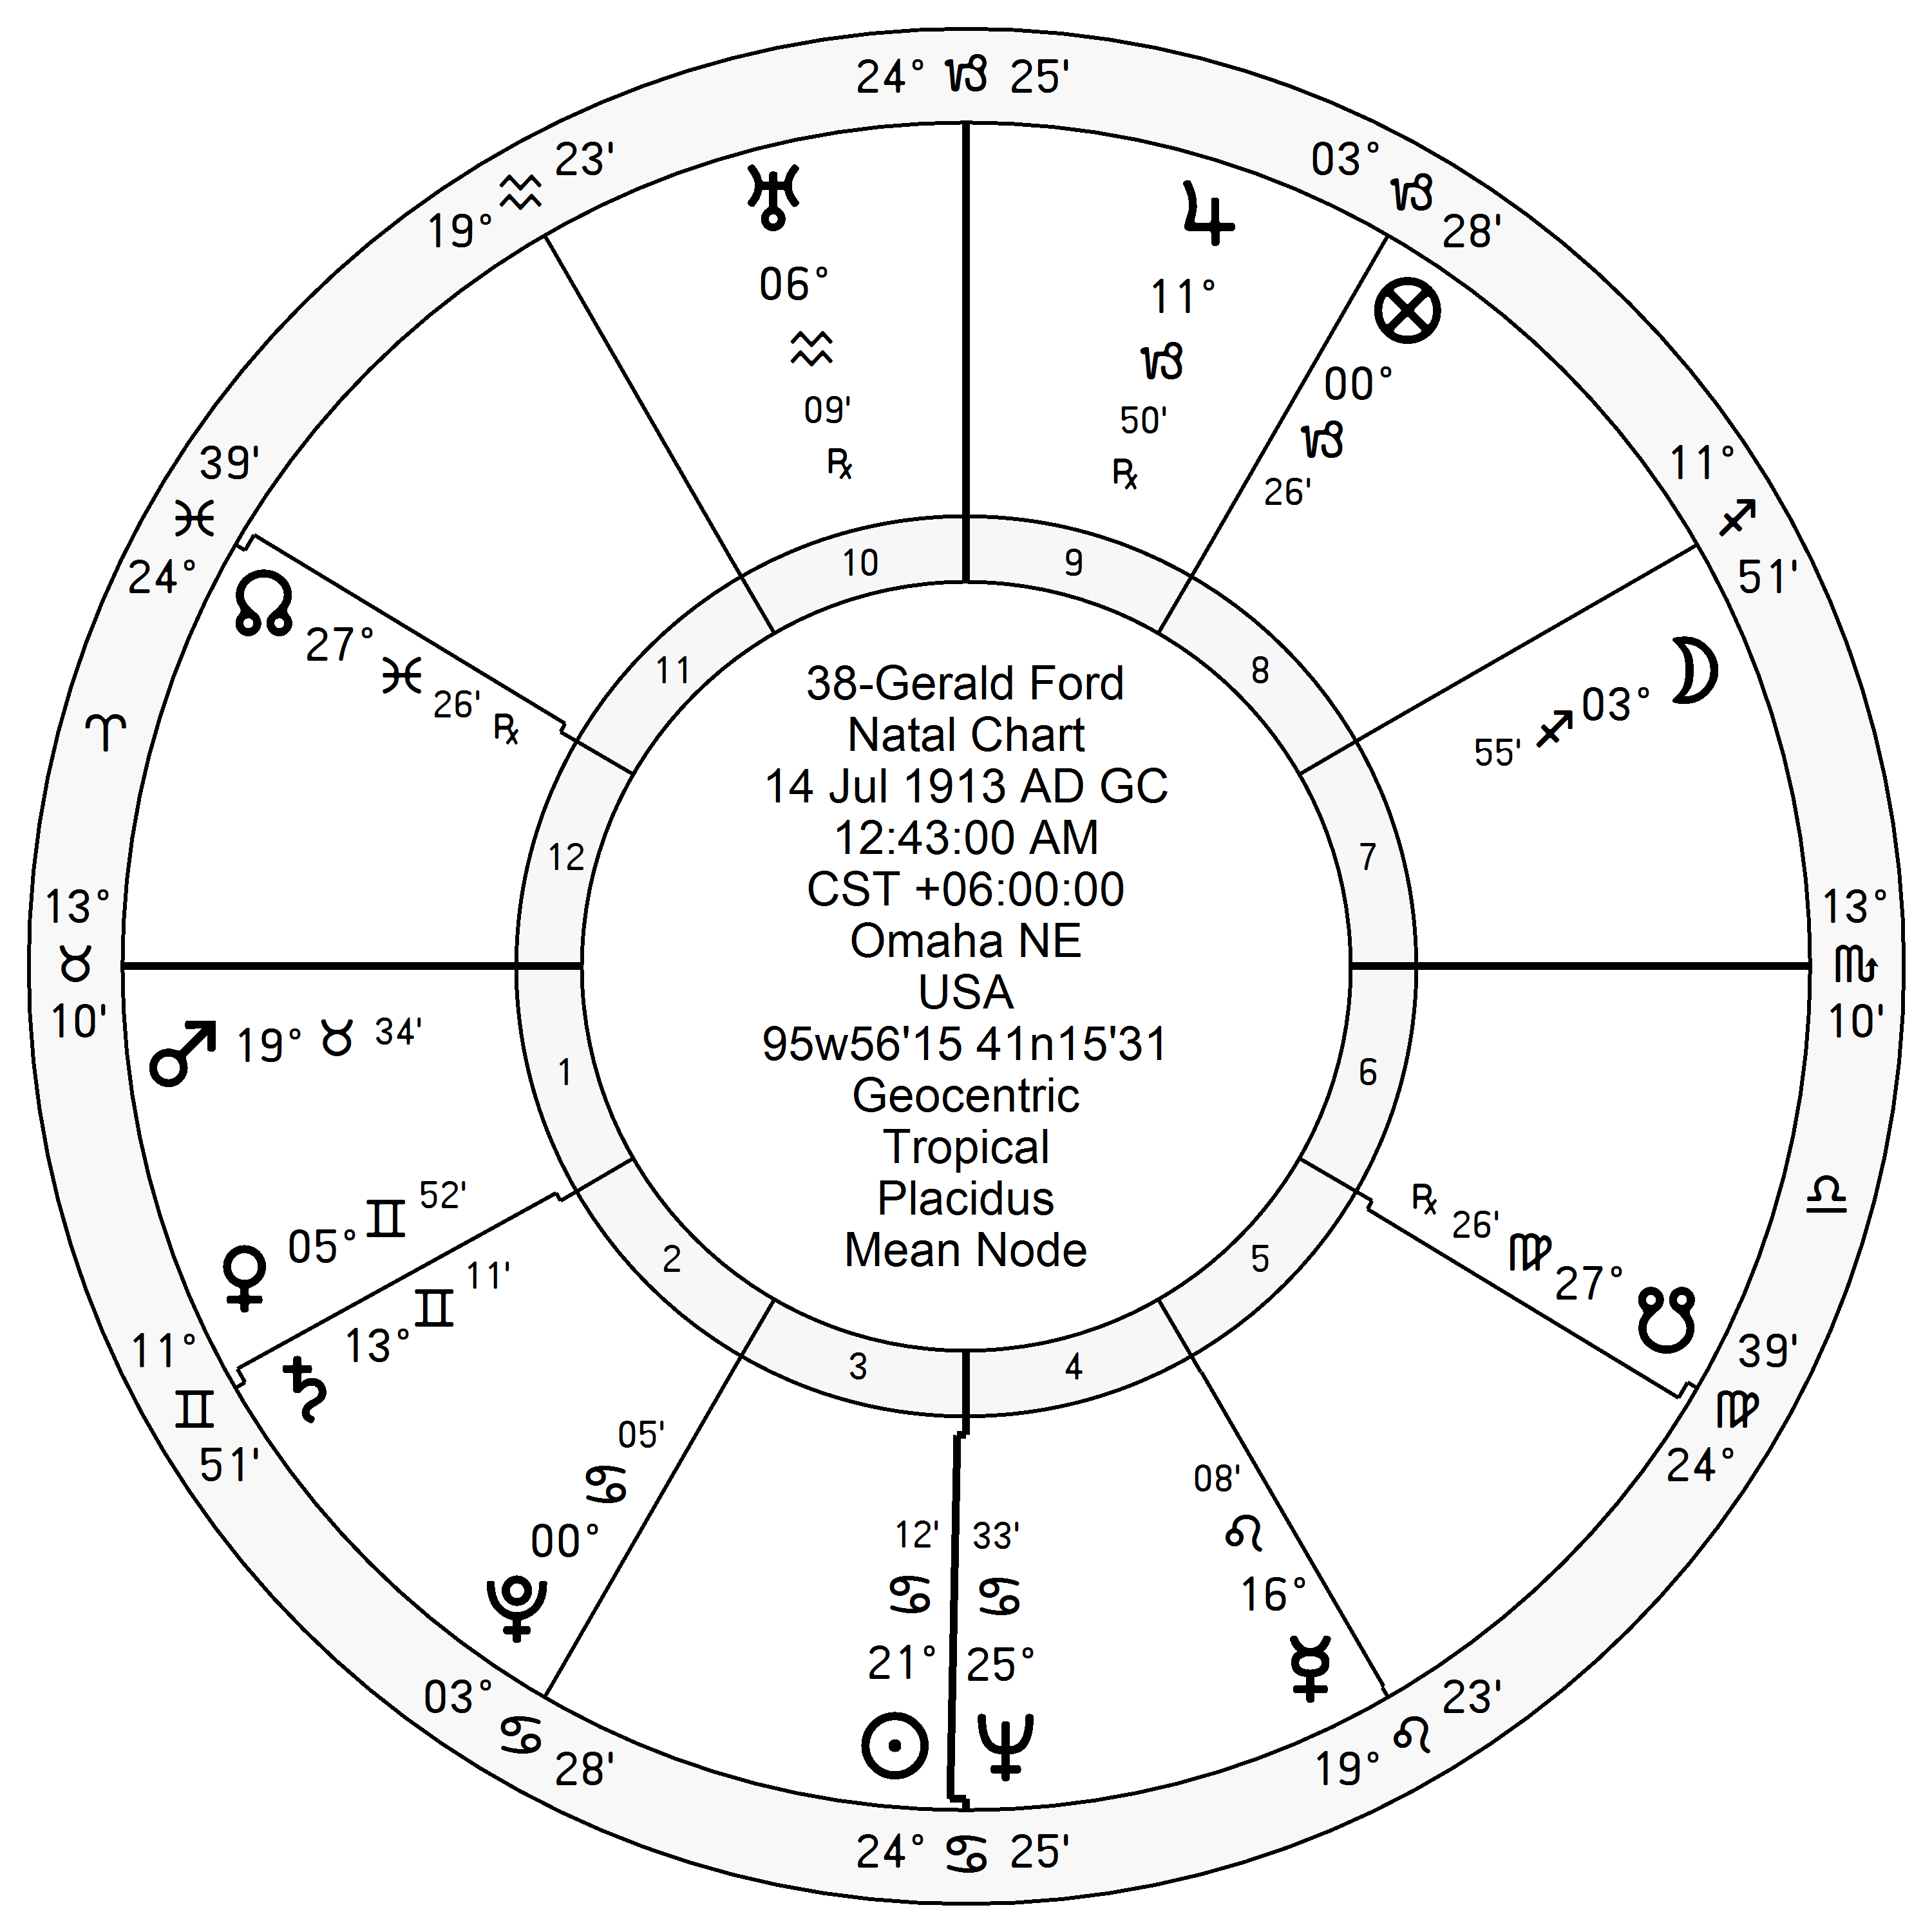
\includegraphics[width=0.9\textwidth]{charts/Ford.png}}
\fontsize{7pt}{8pt}\selectfont

\Sun\, \Sextile\, P10, \Sextile\, N1 \\
\Venus\, in P10, \Square\, P1; \Trine\, N10 \\
\Mars\, in detriment in P10, \Square\, P1; in N1 \Sextile\, N10 \\
\vspace{0.5em}
Carter won by a narrow margin; possibly on the strength of his \Jupiter\, in domicile vs Ford's \Mars\, detriment.

\column{0.48\textwidth}
\vspace{-1em}
{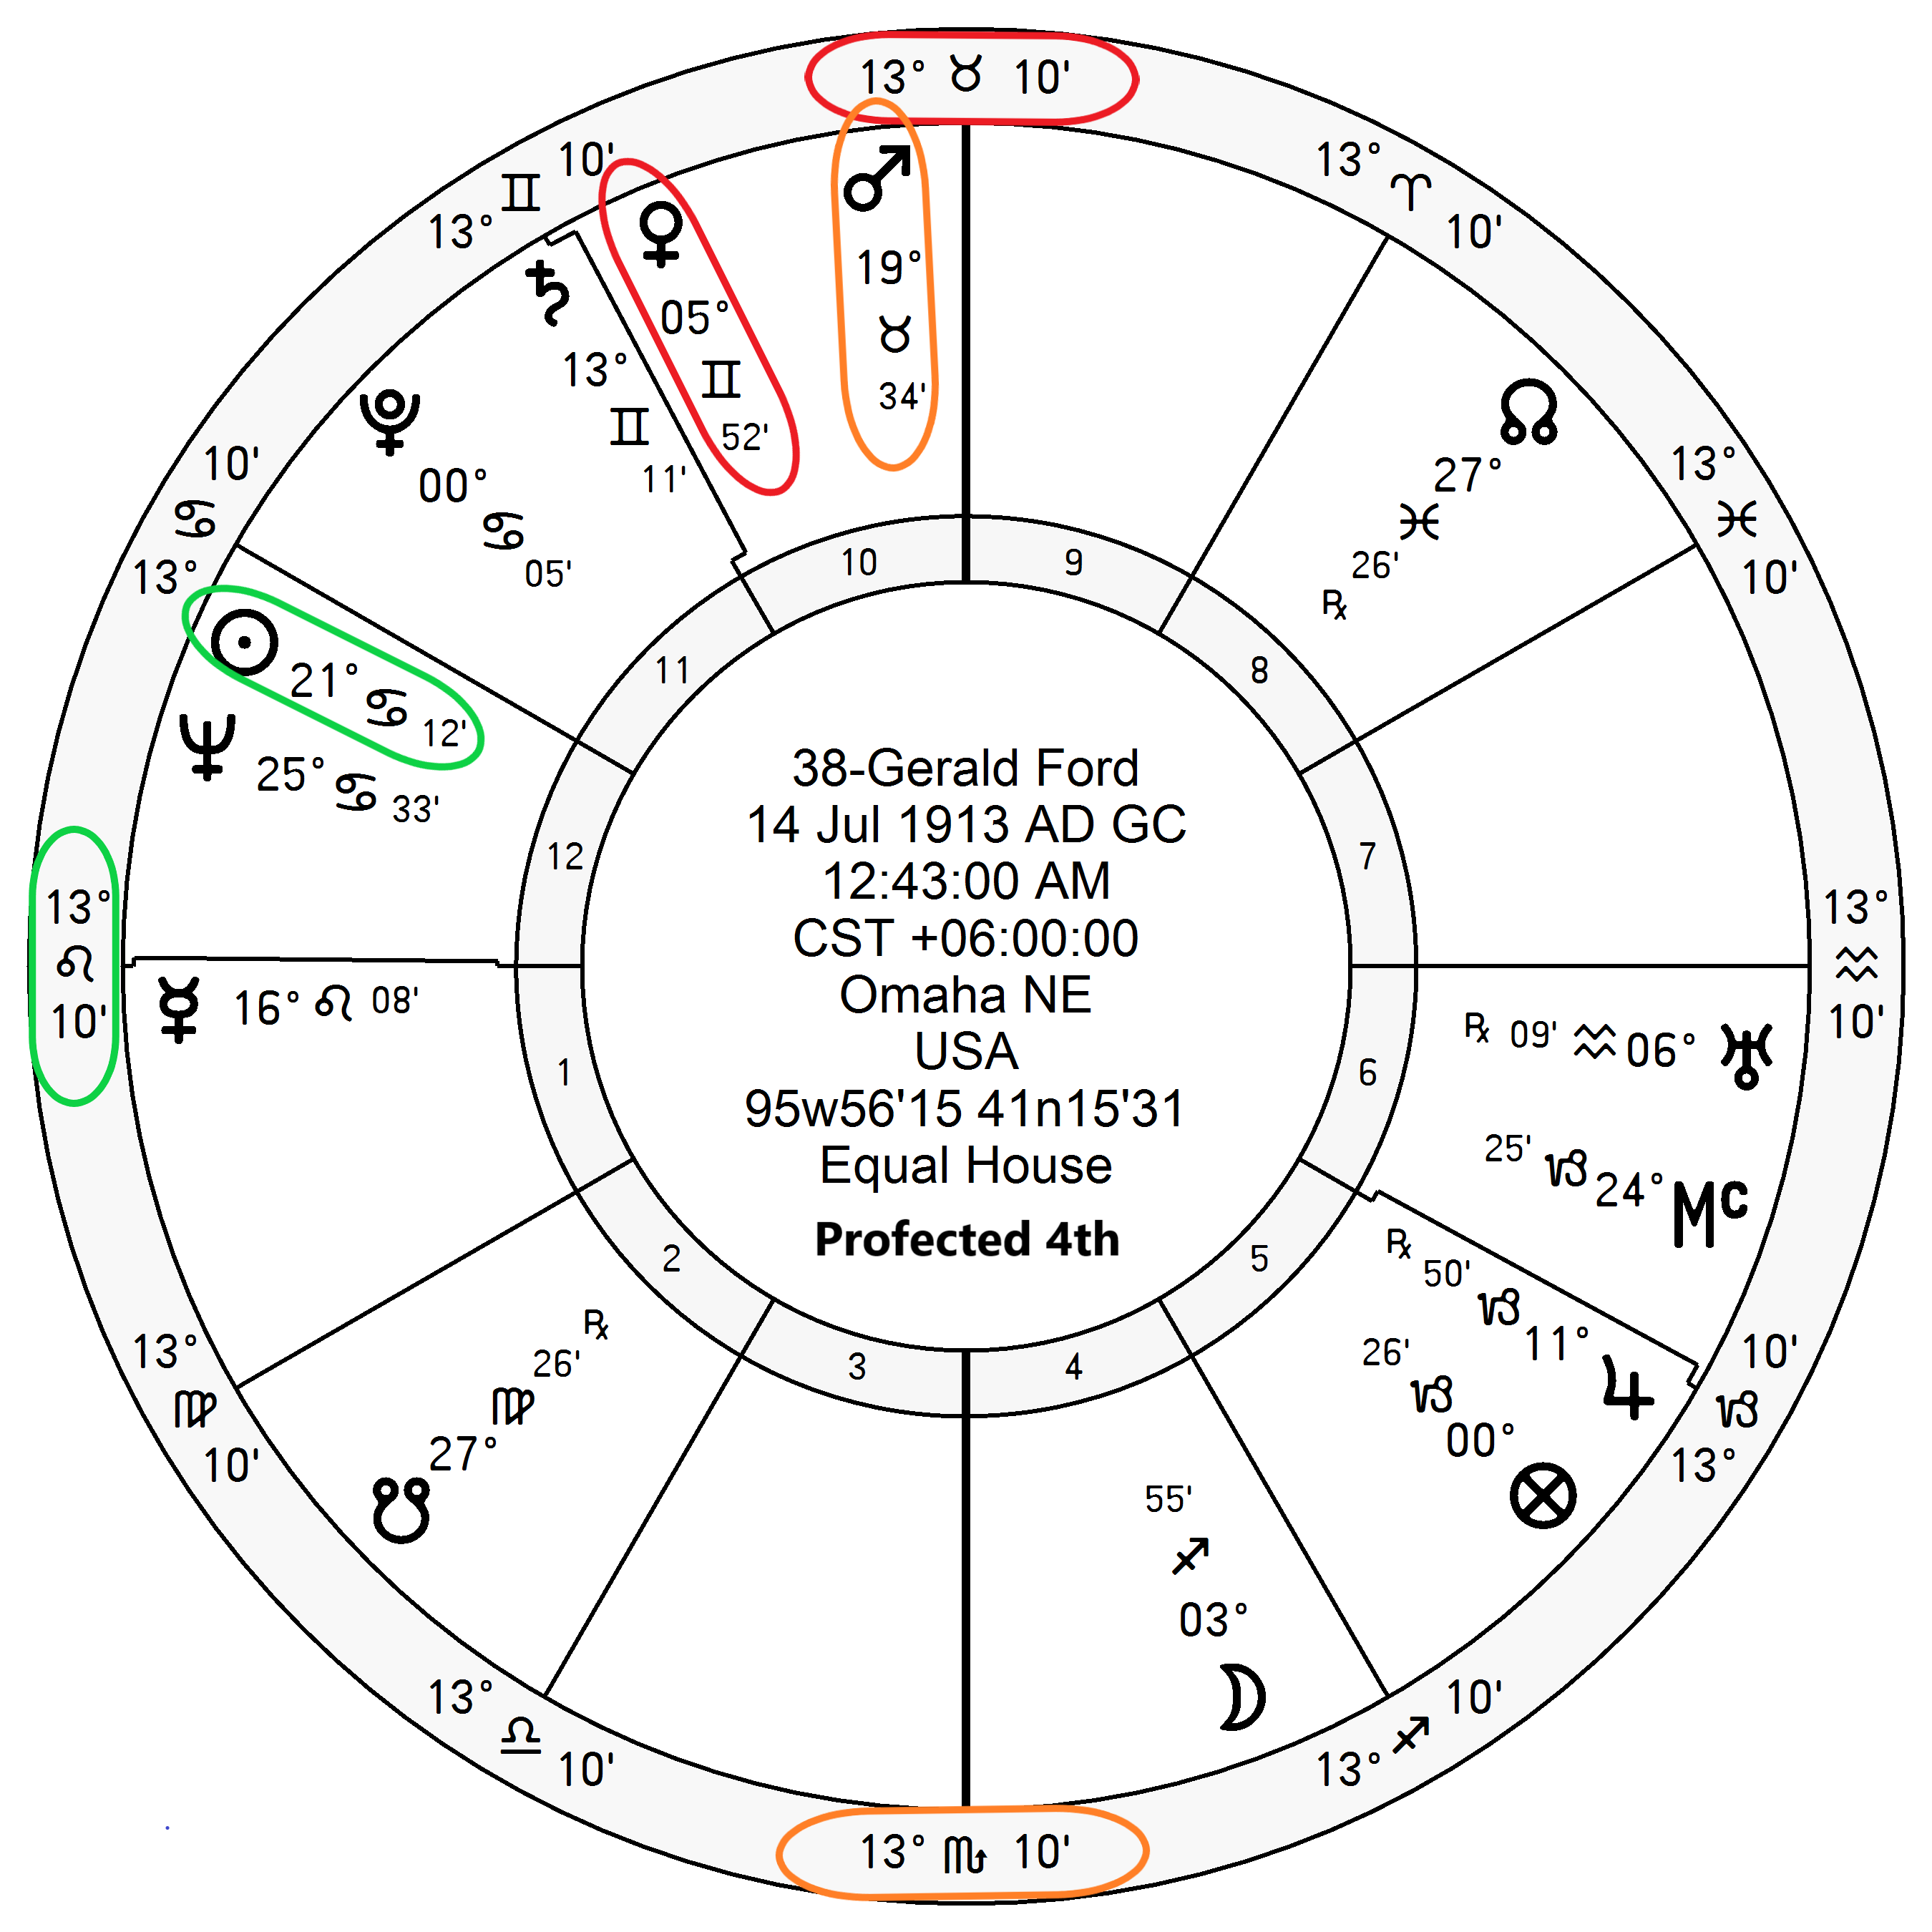
\includegraphics[width=0.9\textwidth]{charts/Ford-Prof-4th.png}}
\fontsize{8pt}{9pt}\selectfont
\textbf{\dgreen P1}=N5
	$\Rightarrow$ \Sun\, $\Rightarrow$ P12/N3\\
\textbf{\red P10=N1}
	$\Rightarrow$ \Venus\, $\Rightarrow$ \textbf{\red P10/N1}\\
PE=P4/N7
	 $\Rightarrow$ \Mars\, $\Rightarrow$ \textbf{\red P10/N1}

\end{columns}
\end{frame}

%\subsection{Election November 4, 1980: *Reagan vs Carter}
\begin{frame}[t]{Election November 4, 1980: *Ronald Reagan}
\small

\begin{columns}[T, onlytextwidth]
\column{0.48\textwidth}
\vspace{-1em}
{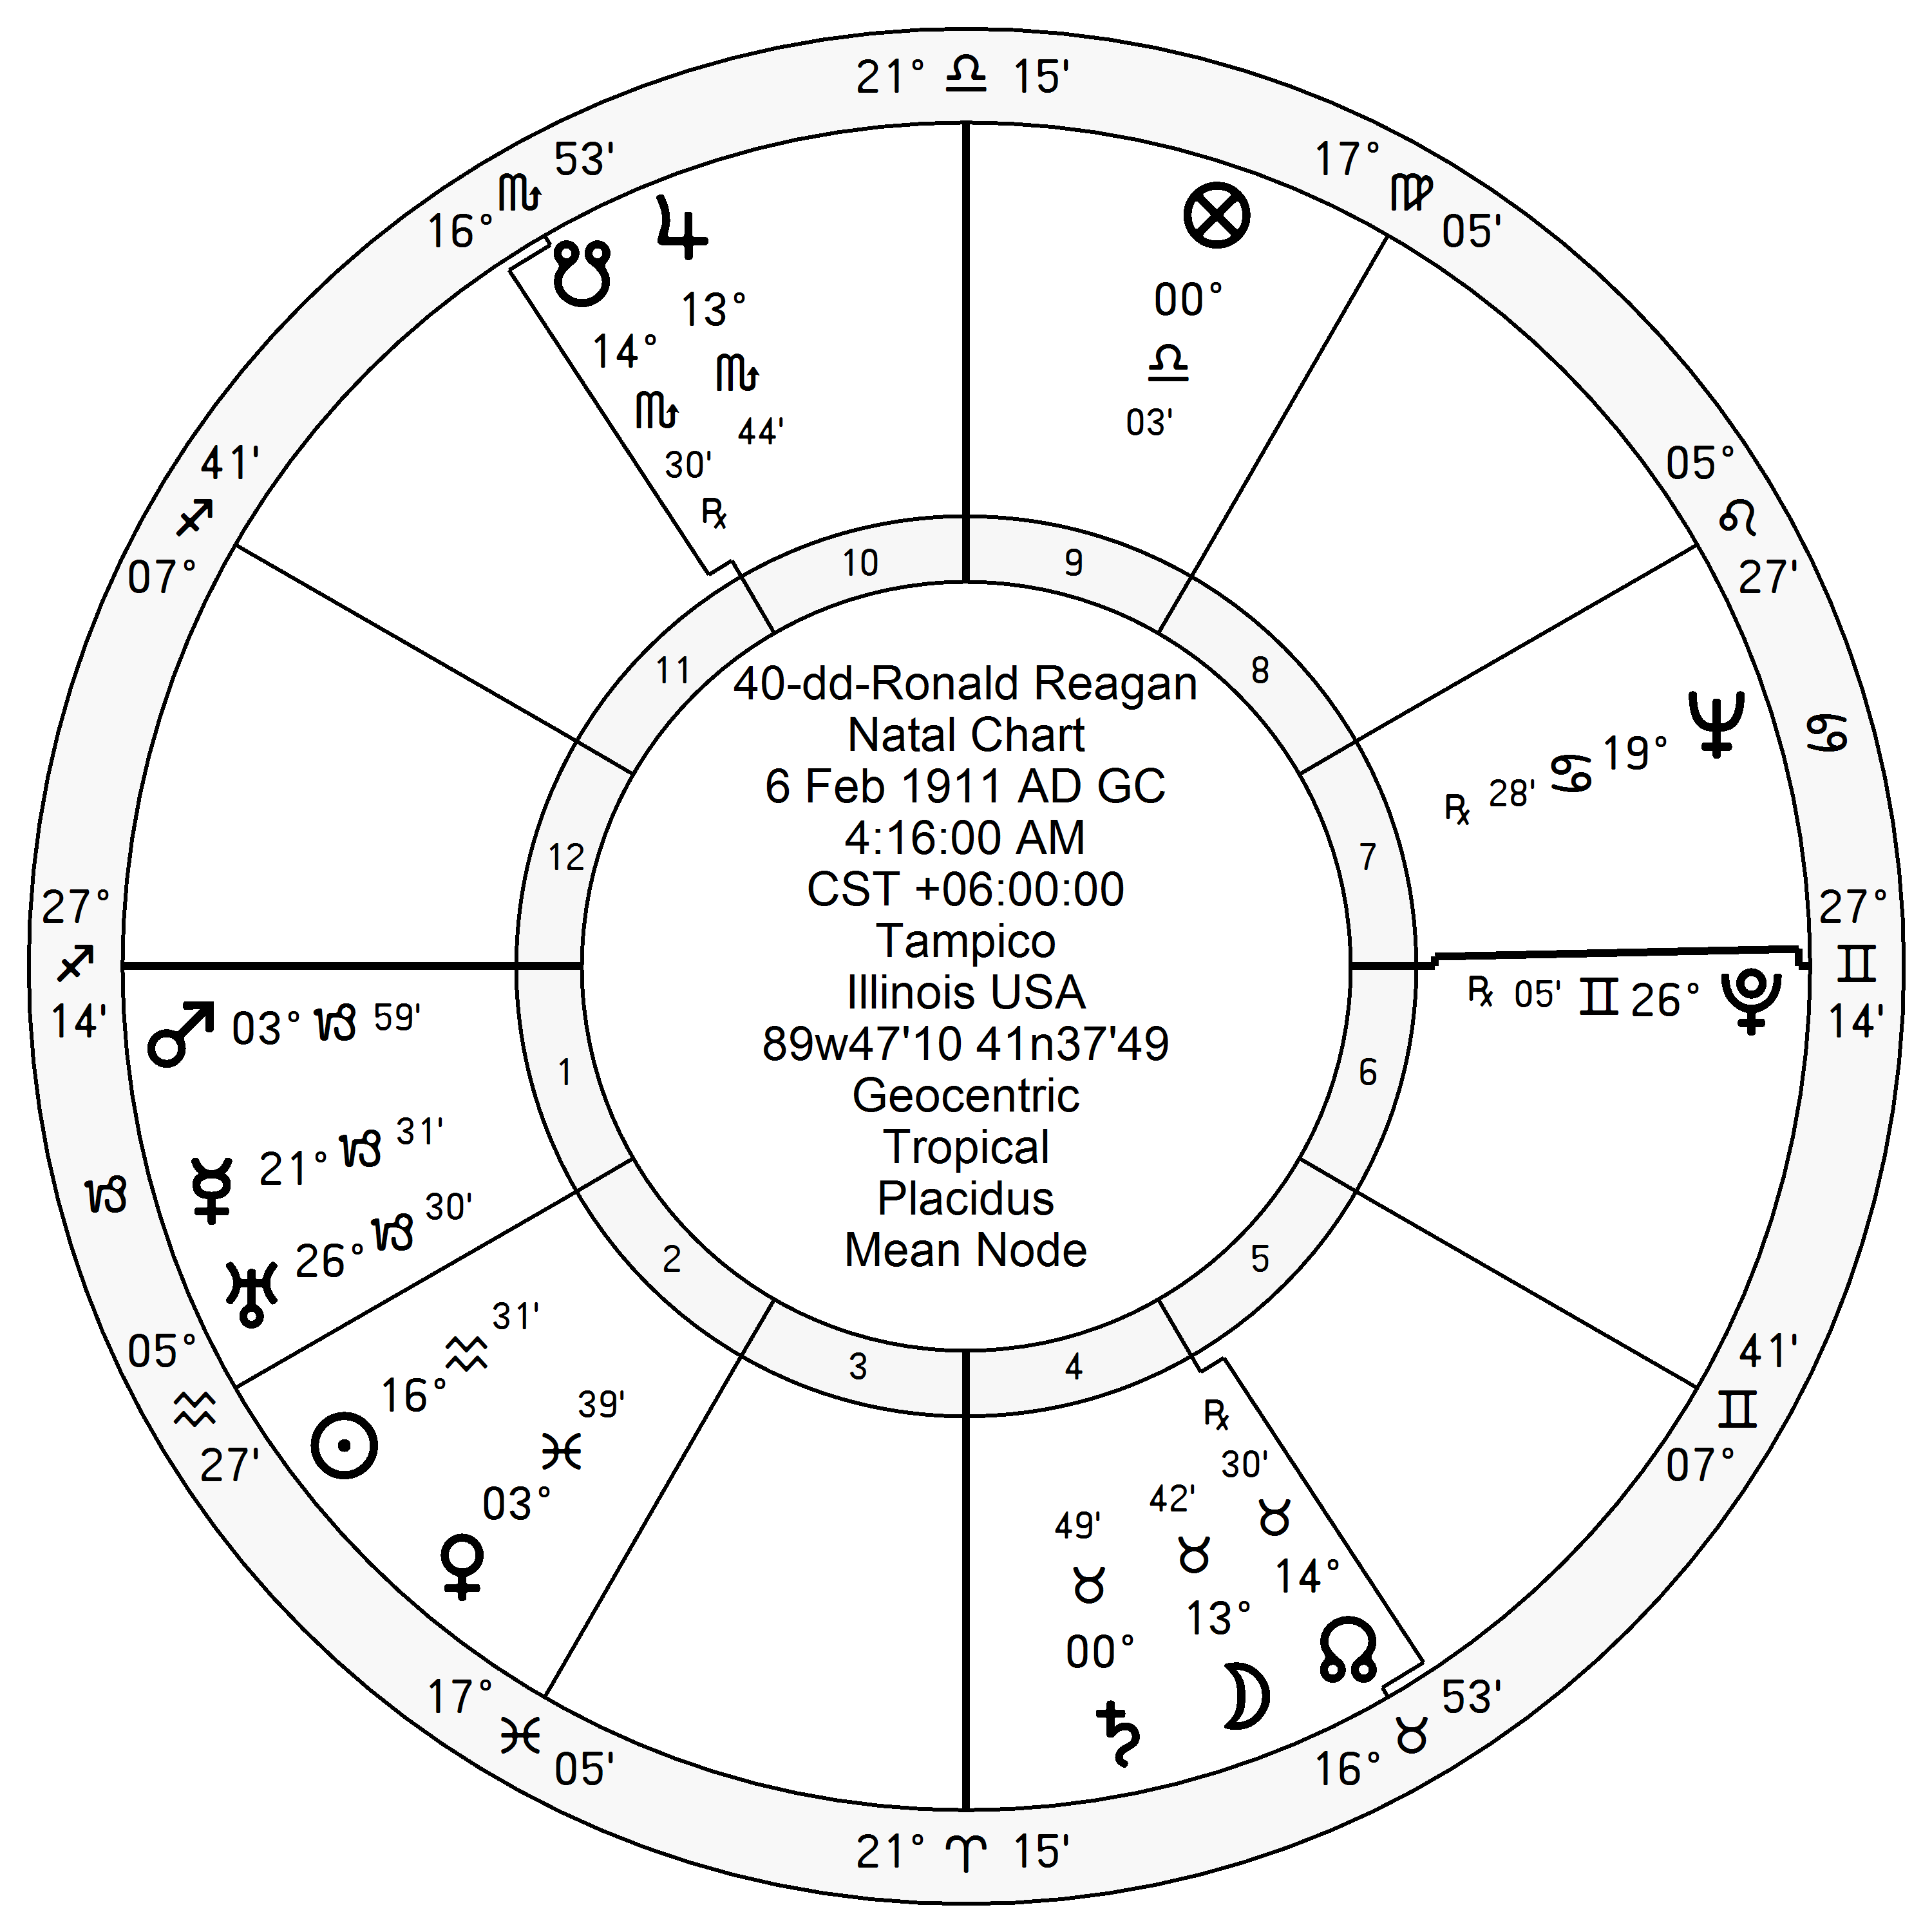
\includegraphics[width=0.9\textwidth]{charts/Reagan-dd.png}}
\fontsize{8pt}{9pt}\selectfont

\Mercury\, \Opposition\, P10, \Square\, P1; in N1 partile \Square\, MC \\
\Venus\, \Trine\, P10, \Trine\, N10

\column{0.48\textwidth}
\vspace{-1em}
{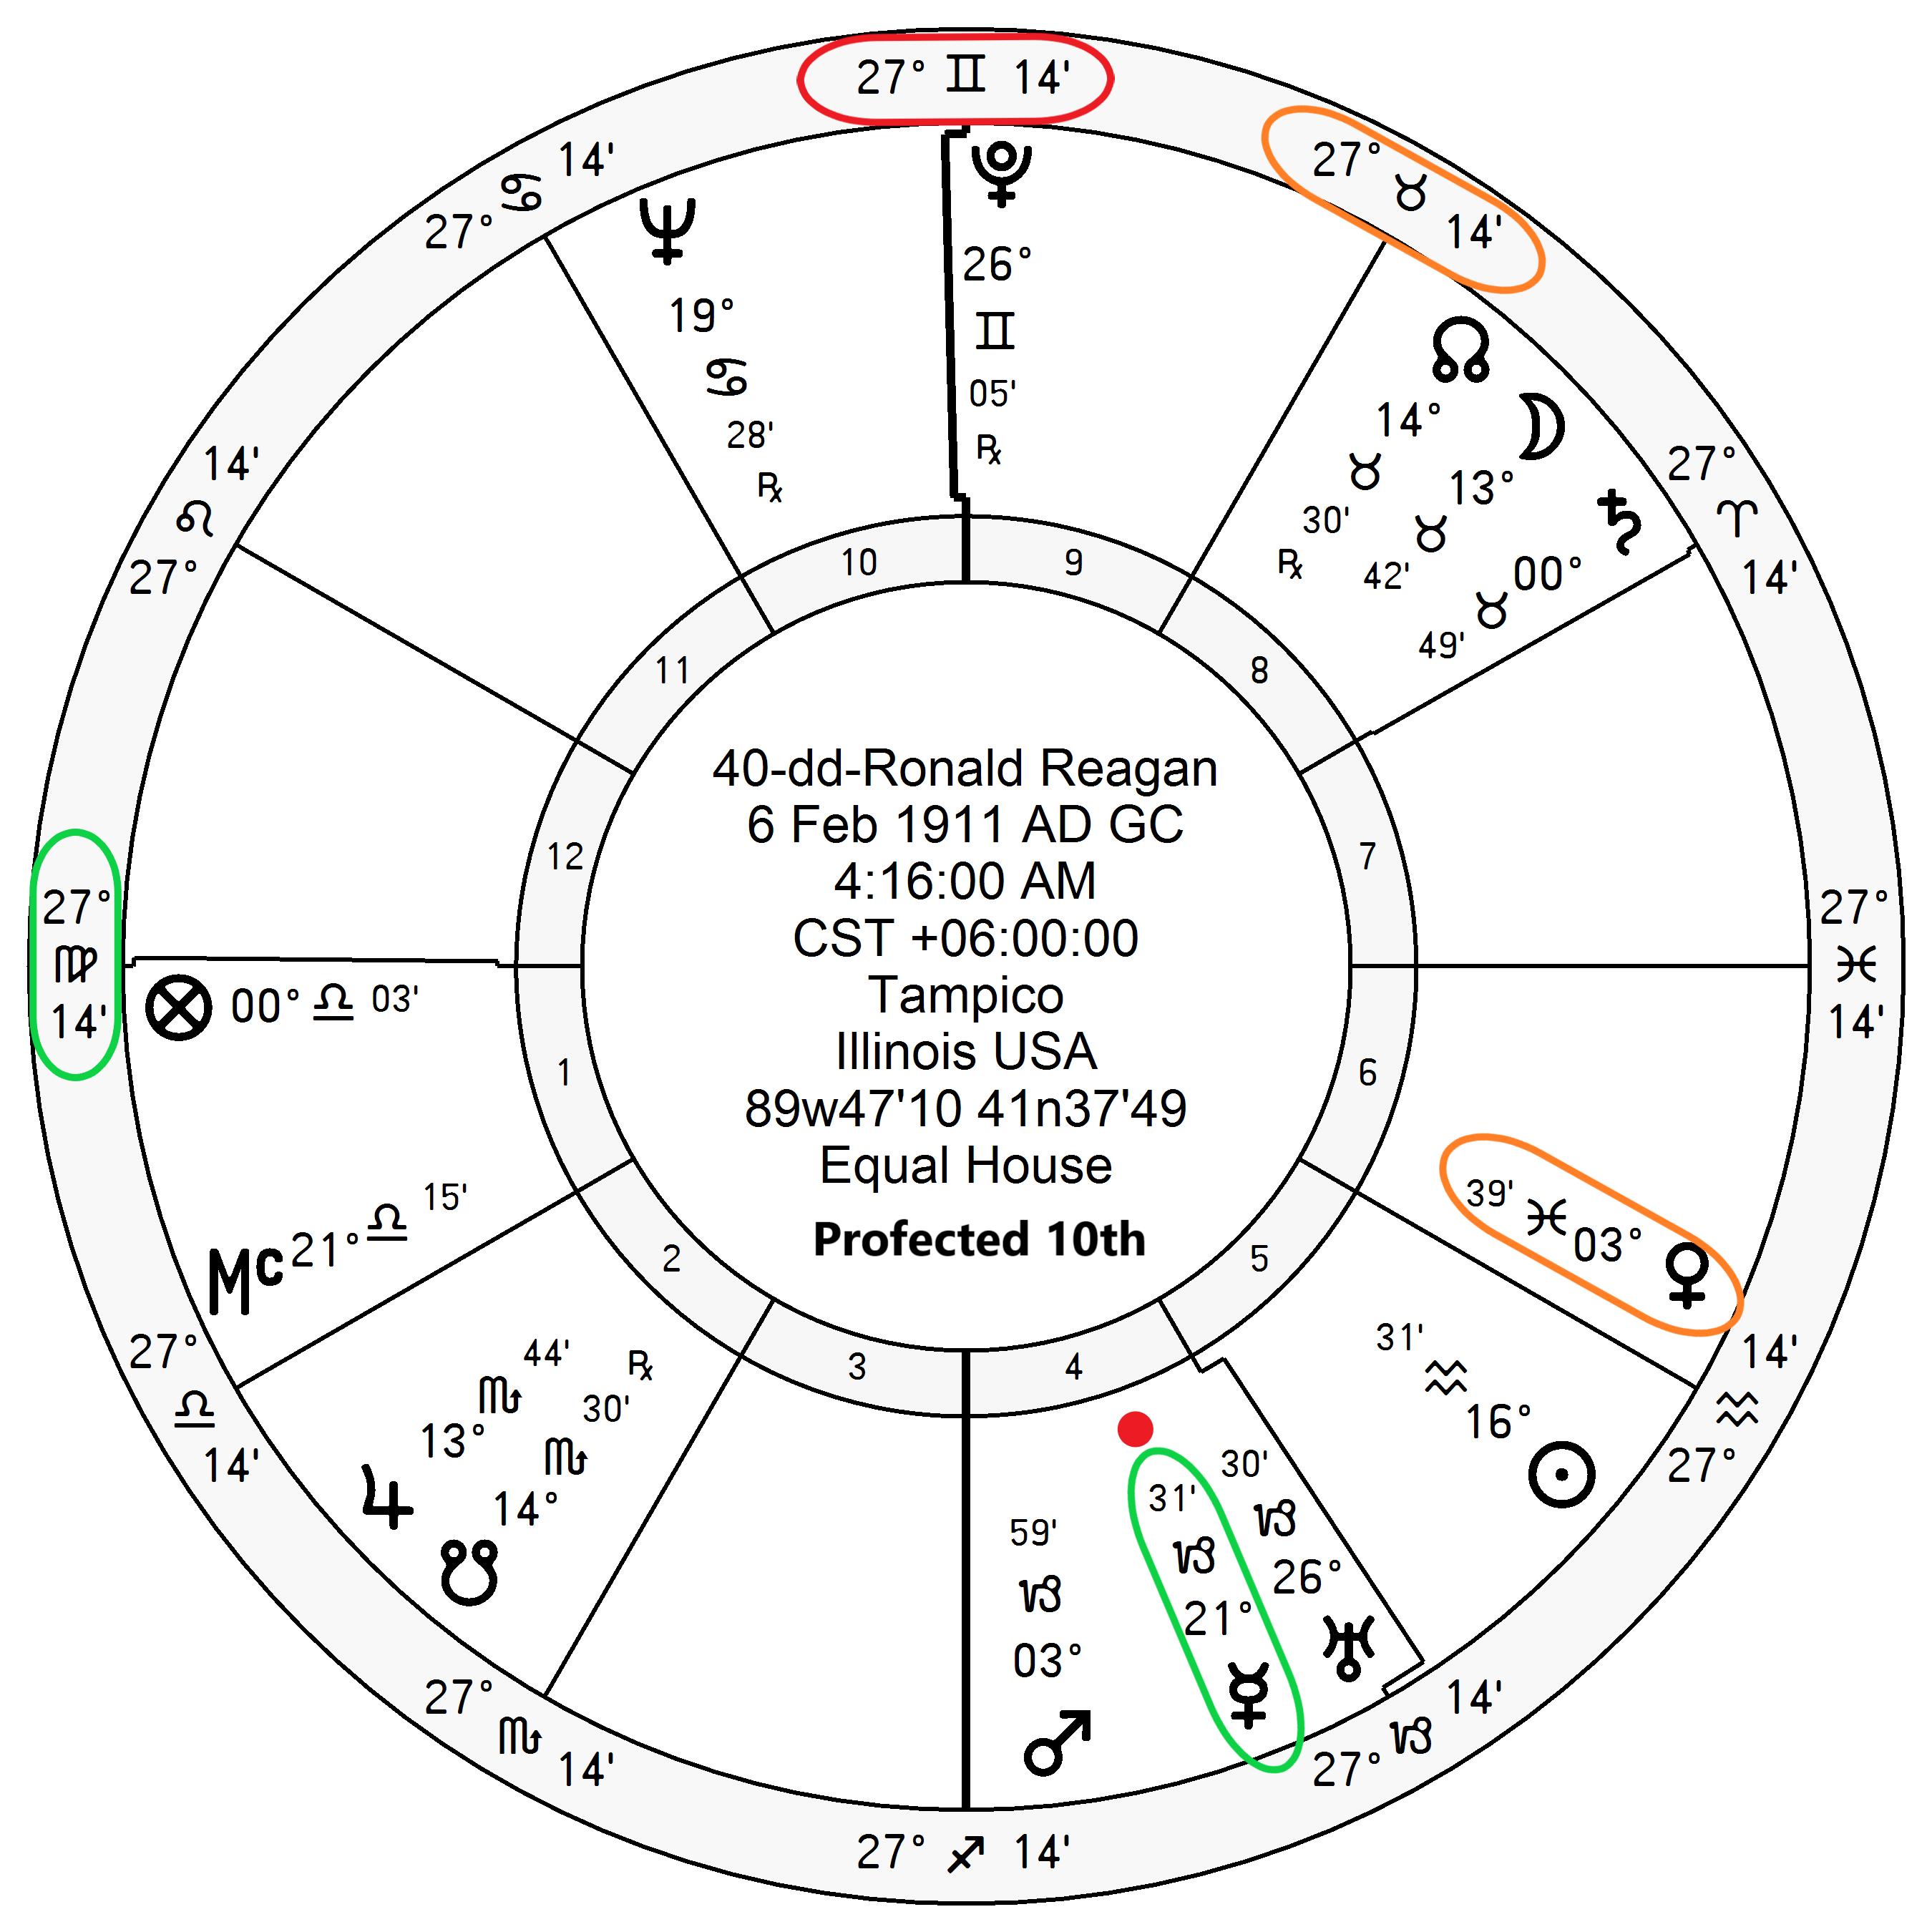
\includegraphics[width=0.9\textwidth]{charts/Reagan-dd-Prof-10th.png}}
\fontsize{8pt}{9pt}\selectfont

\textbf{\dgreen P1=N9} 
	$\Rightarrow$ \Mercury\, $\Rightarrow$ \textbf{\dgreen P4/N1}\\
\textbf{\red P10=N6}
	$\Rightarrow$ \Mercury\, $\Rightarrow$ \textbf{\dgreen P4/N1}\\
PE=\textbf{\dgreen P9}/N5
	 $\Rightarrow$ \Venus\, $\Rightarrow$ \textbf{\red P6}/N2

\end{columns}
\end{frame}

% ===================================================
\begin{frame}[t]{Election November 4, 1980: Jimmy Carter}
\small
\begin{columns}[T, onlytextwidth]
\column{0.48\textwidth}
\vspace{-1em}
{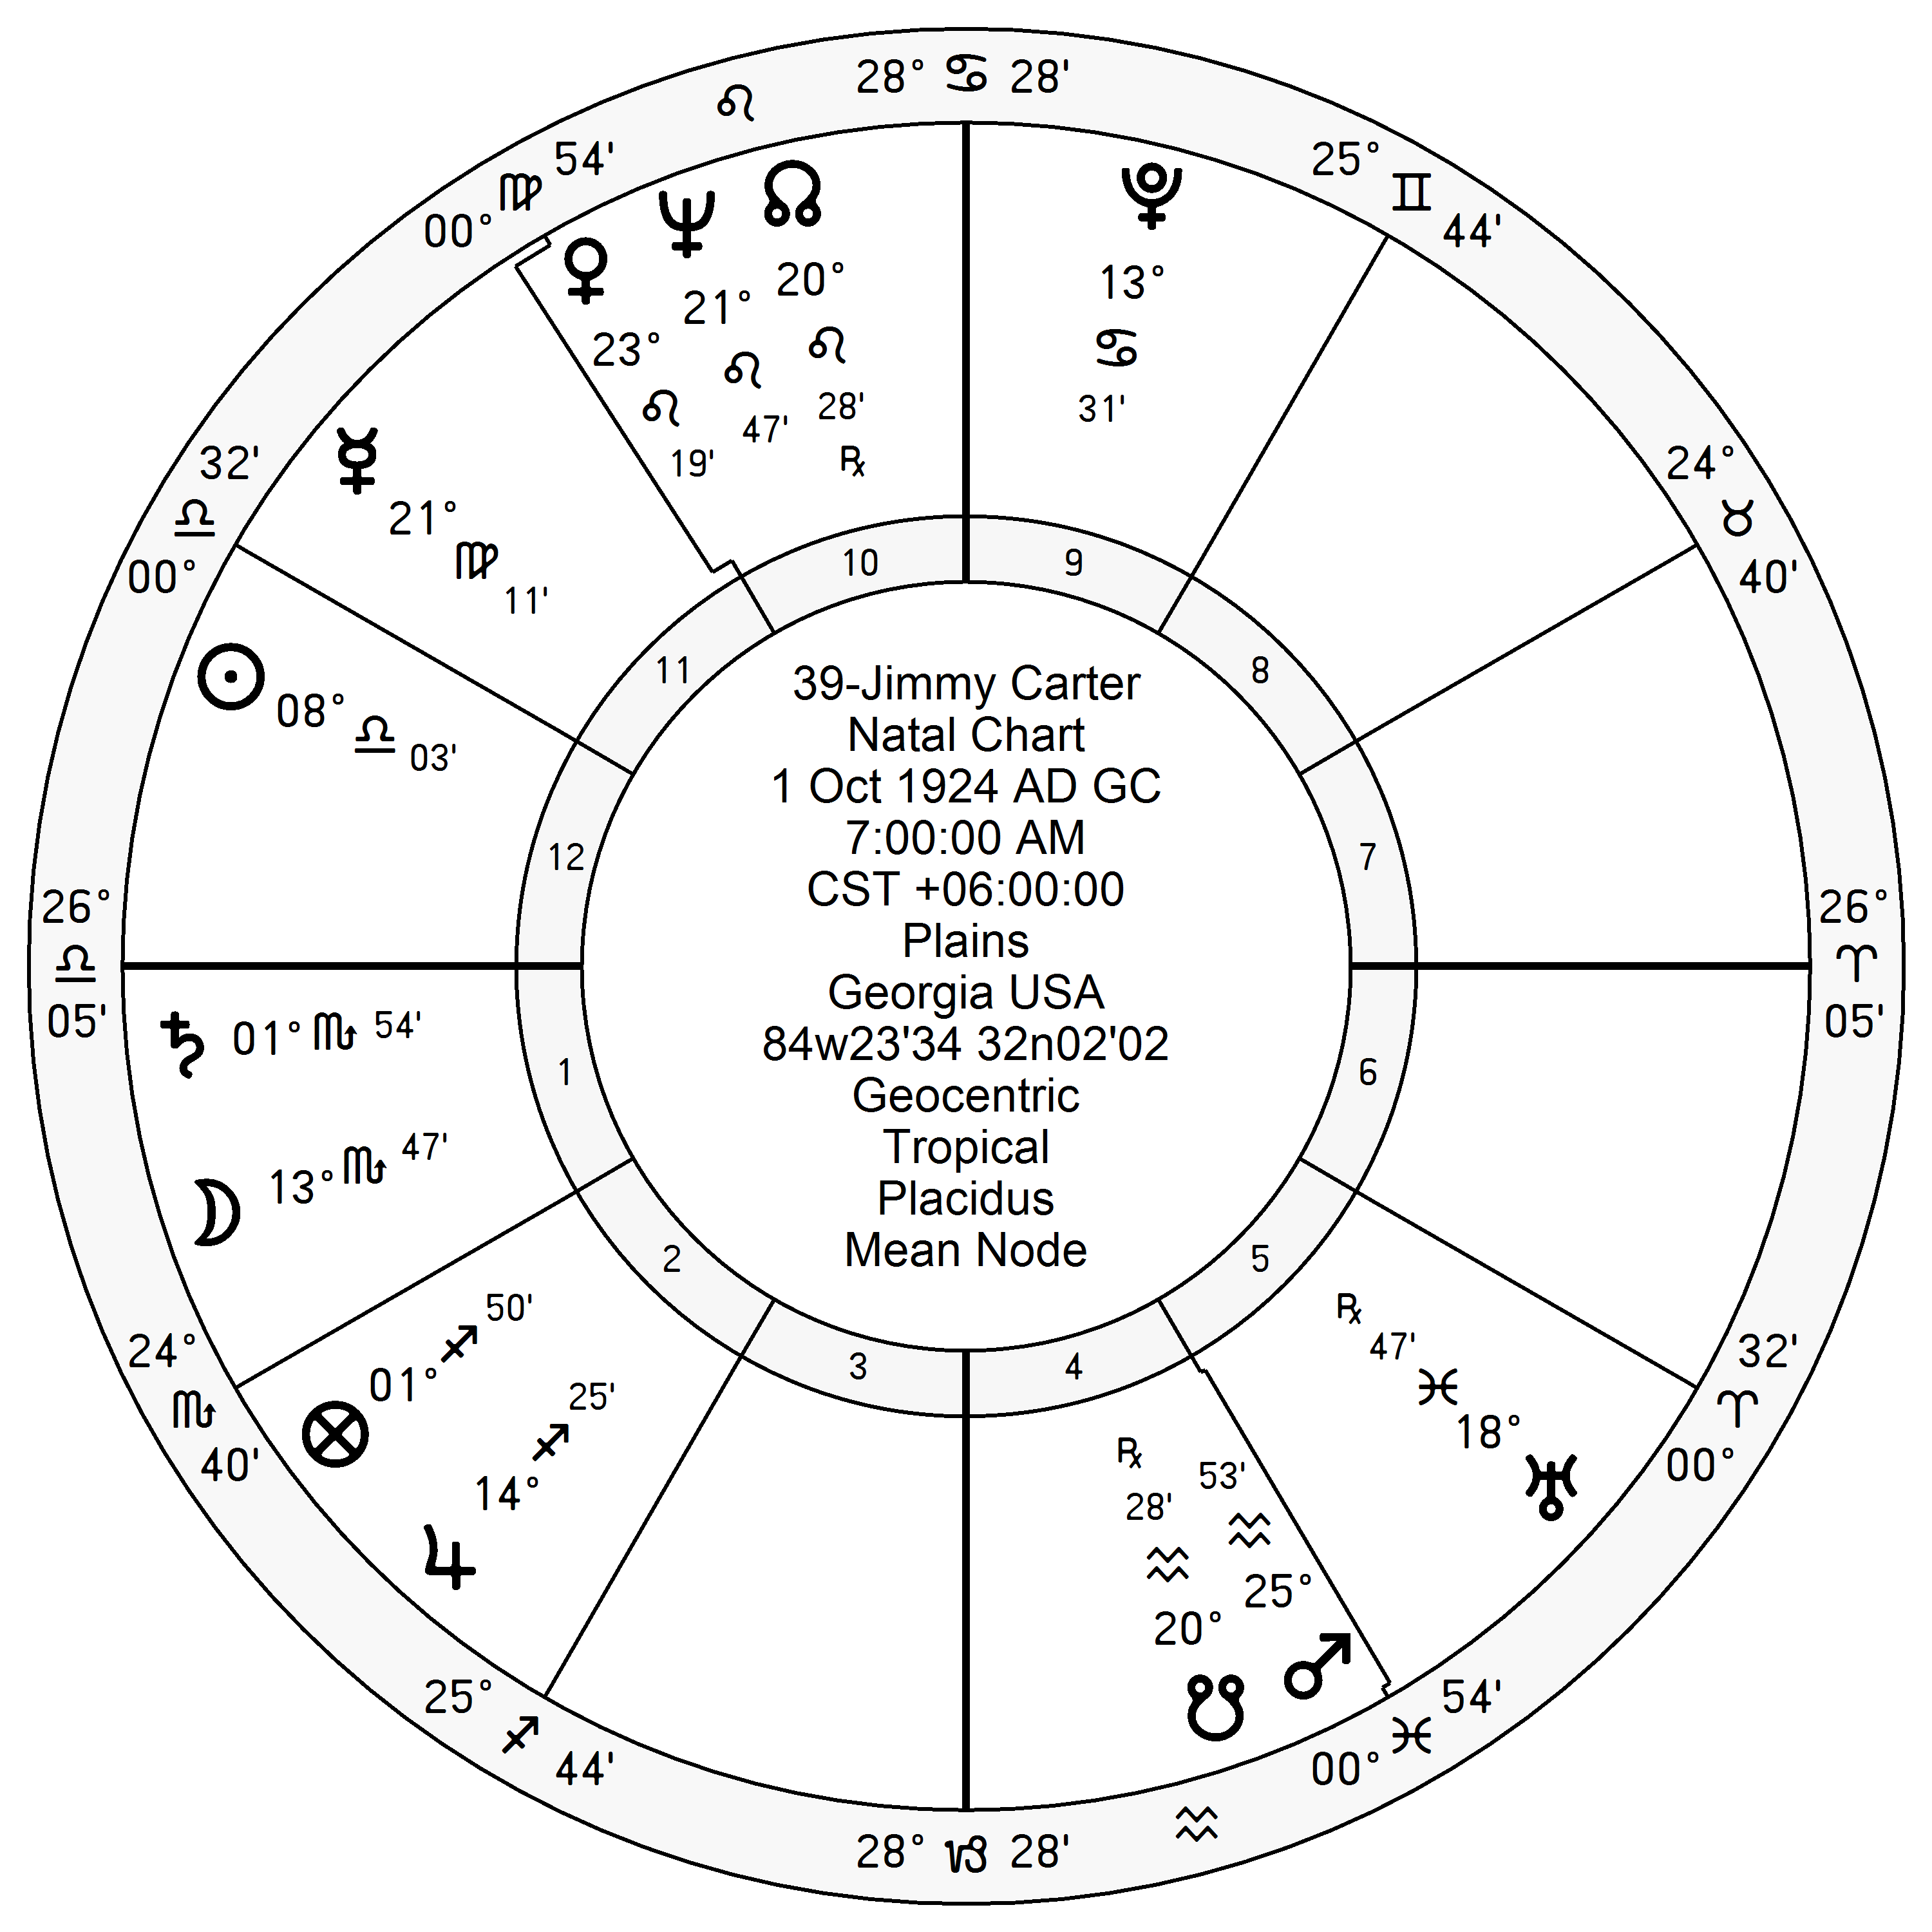
\includegraphics[width=0.9\textwidth]{charts/Carter.png}}
\fontsize{8pt}{9pt}\selectfont

\Mercury\, \Sextile\, P1; \Sextile\, N1 \\
\Jupiter\, \Trine\, P10, \Trine\, N10 \\
\Moon\, \Trine\, P1; in N1 \Square\, N10

\column{0.48\textwidth}
\vspace{-1em}
{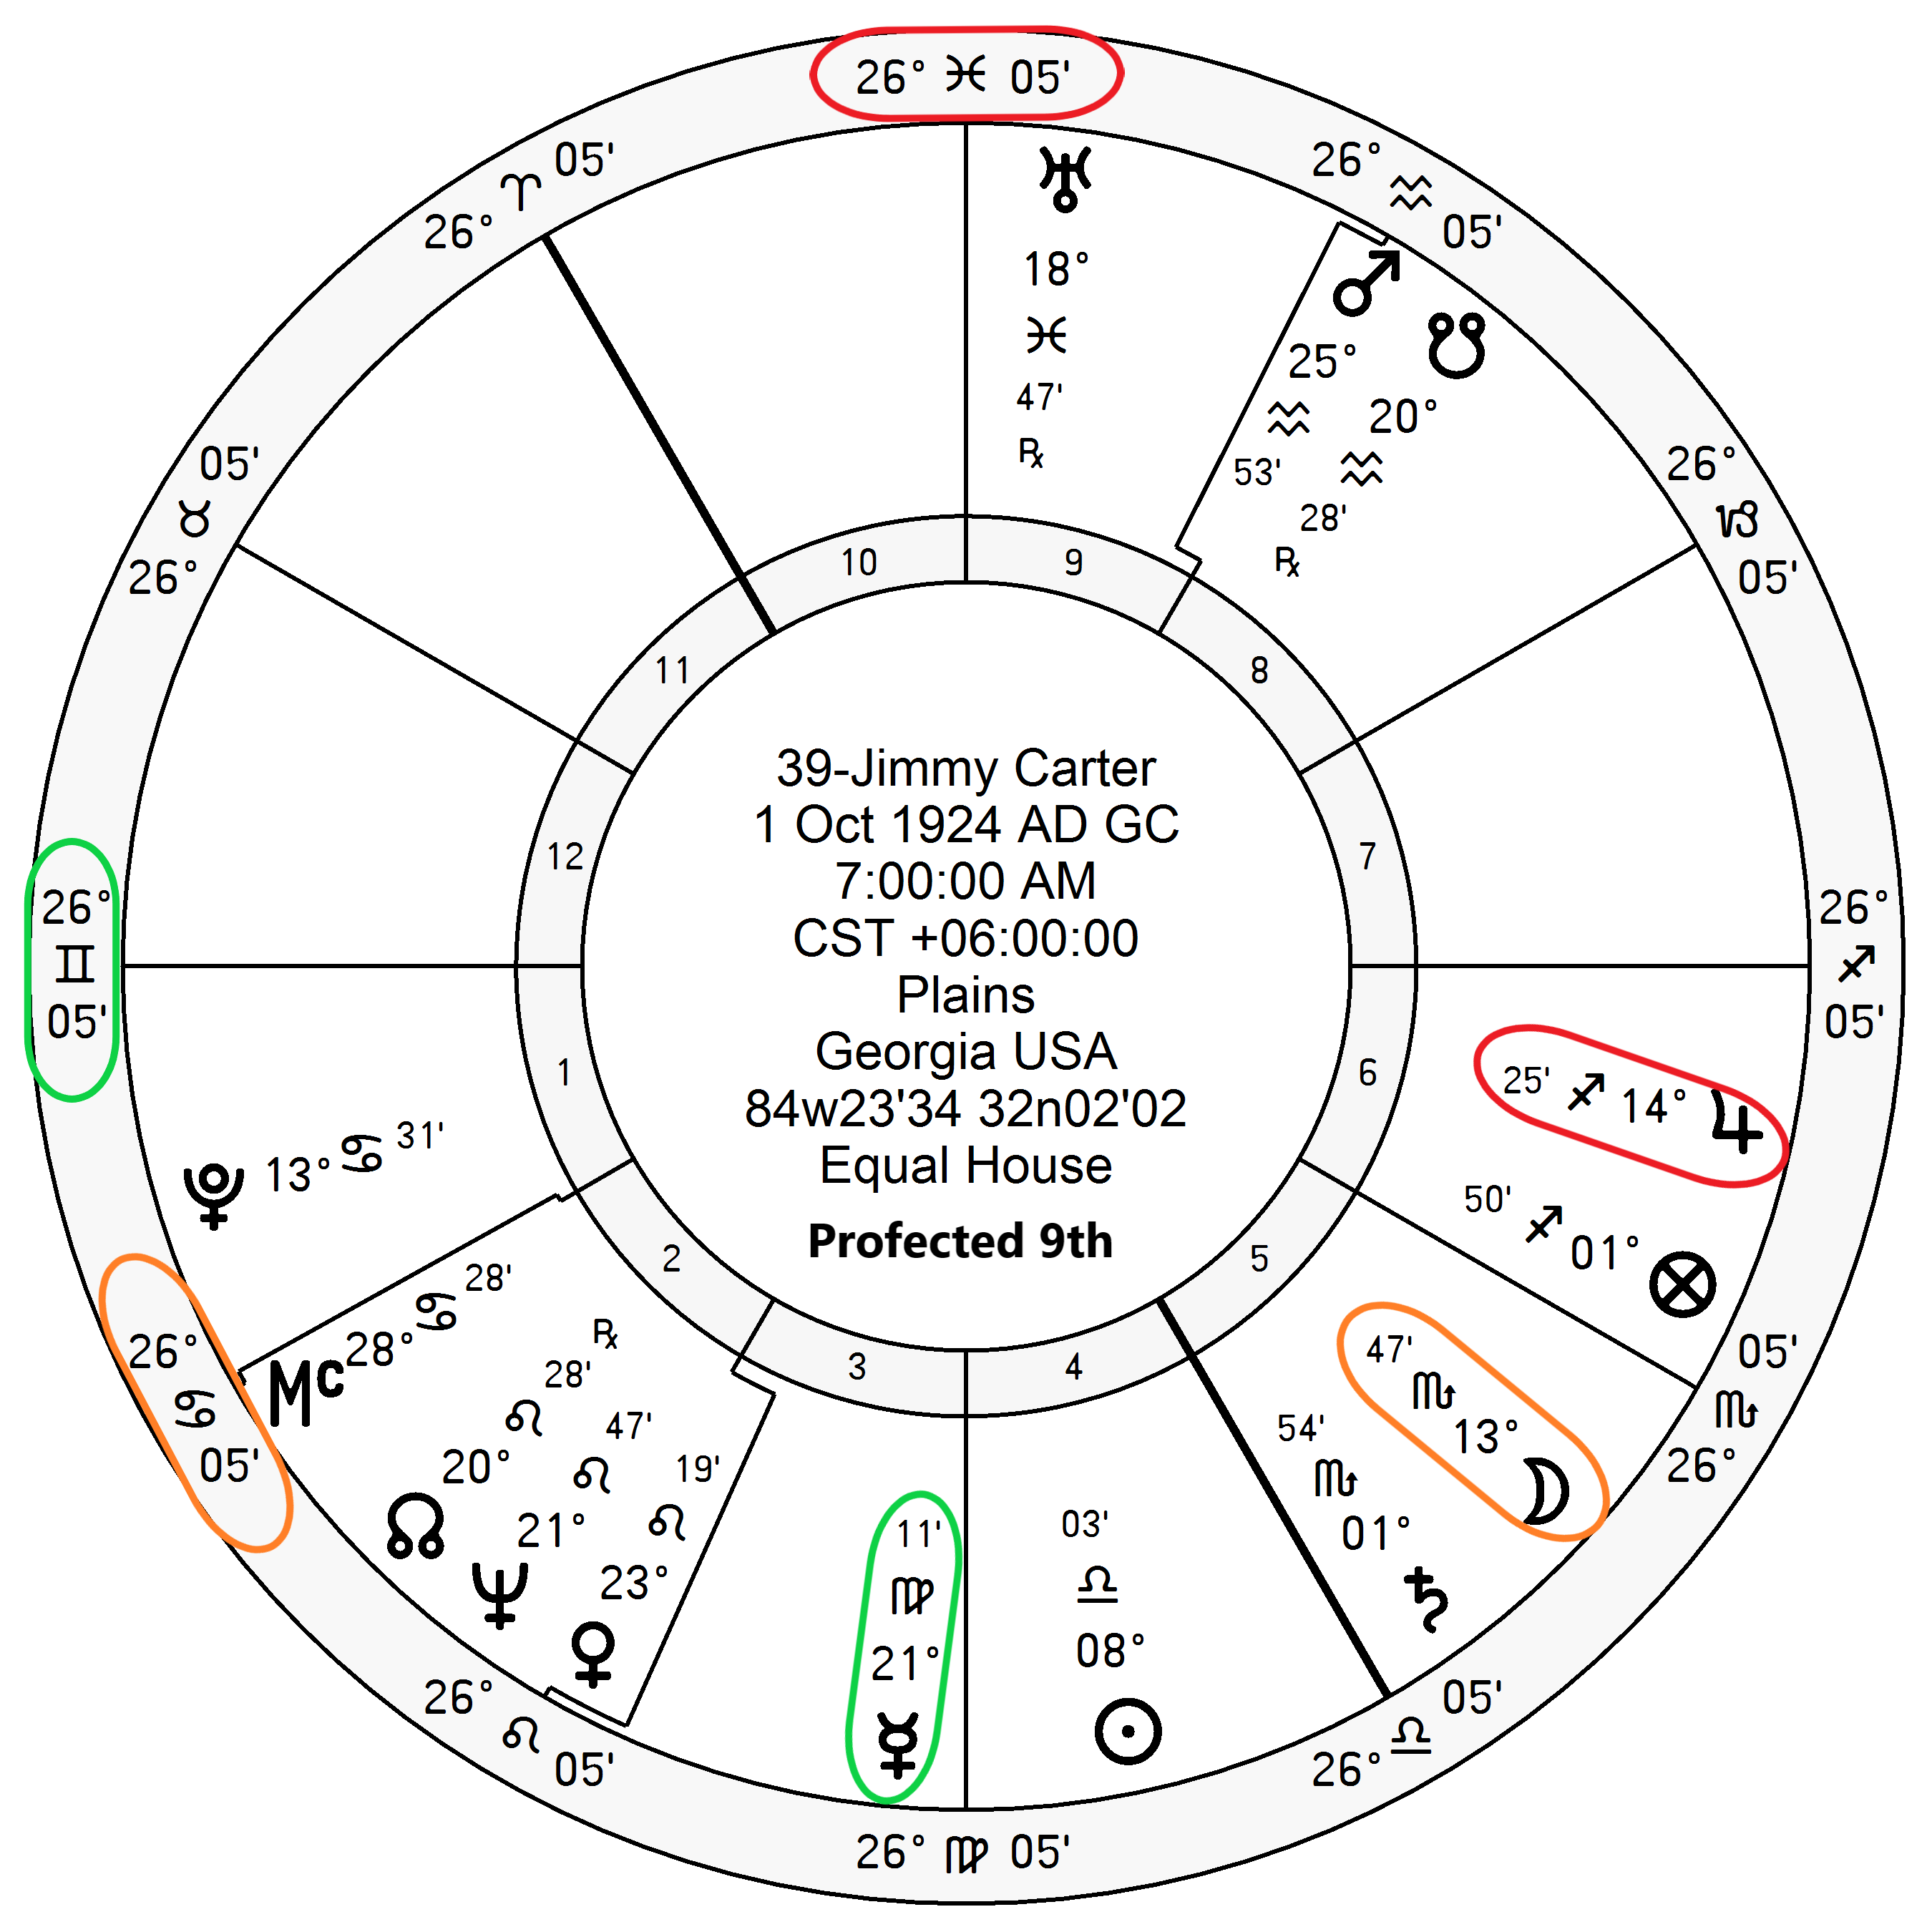
\includegraphics[width=0.9\textwidth]{charts/Carter-Prof-9th.png}}
\fontsize{8pt}{9pt}\selectfont
\textbf{\dgreen P1}=N9
	$\Rightarrow$ \Mercury\, $\Rightarrow$ P3/N11\\
\textbf{\red P10=N5}
	$\Rightarrow$ \Jupiter\, $\Rightarrow$ P6/N2\\
PE=P2/\textbf{\red N10}
	 $\Rightarrow$ \Moon\, $\Rightarrow$ \textbf{\red P5}/\textbf{\dgreen N1}

\end{columns}
\end{frame}

%\subsection{Election November 6, 1984: *Reagan vs Mondale}
\begin{frame}[t]{Election November 6, 1984: *Ronald Reagan}
\small

\begin{columns}[T, onlytextwidth]
\column{0.48\textwidth}
\vspace{-1em}
{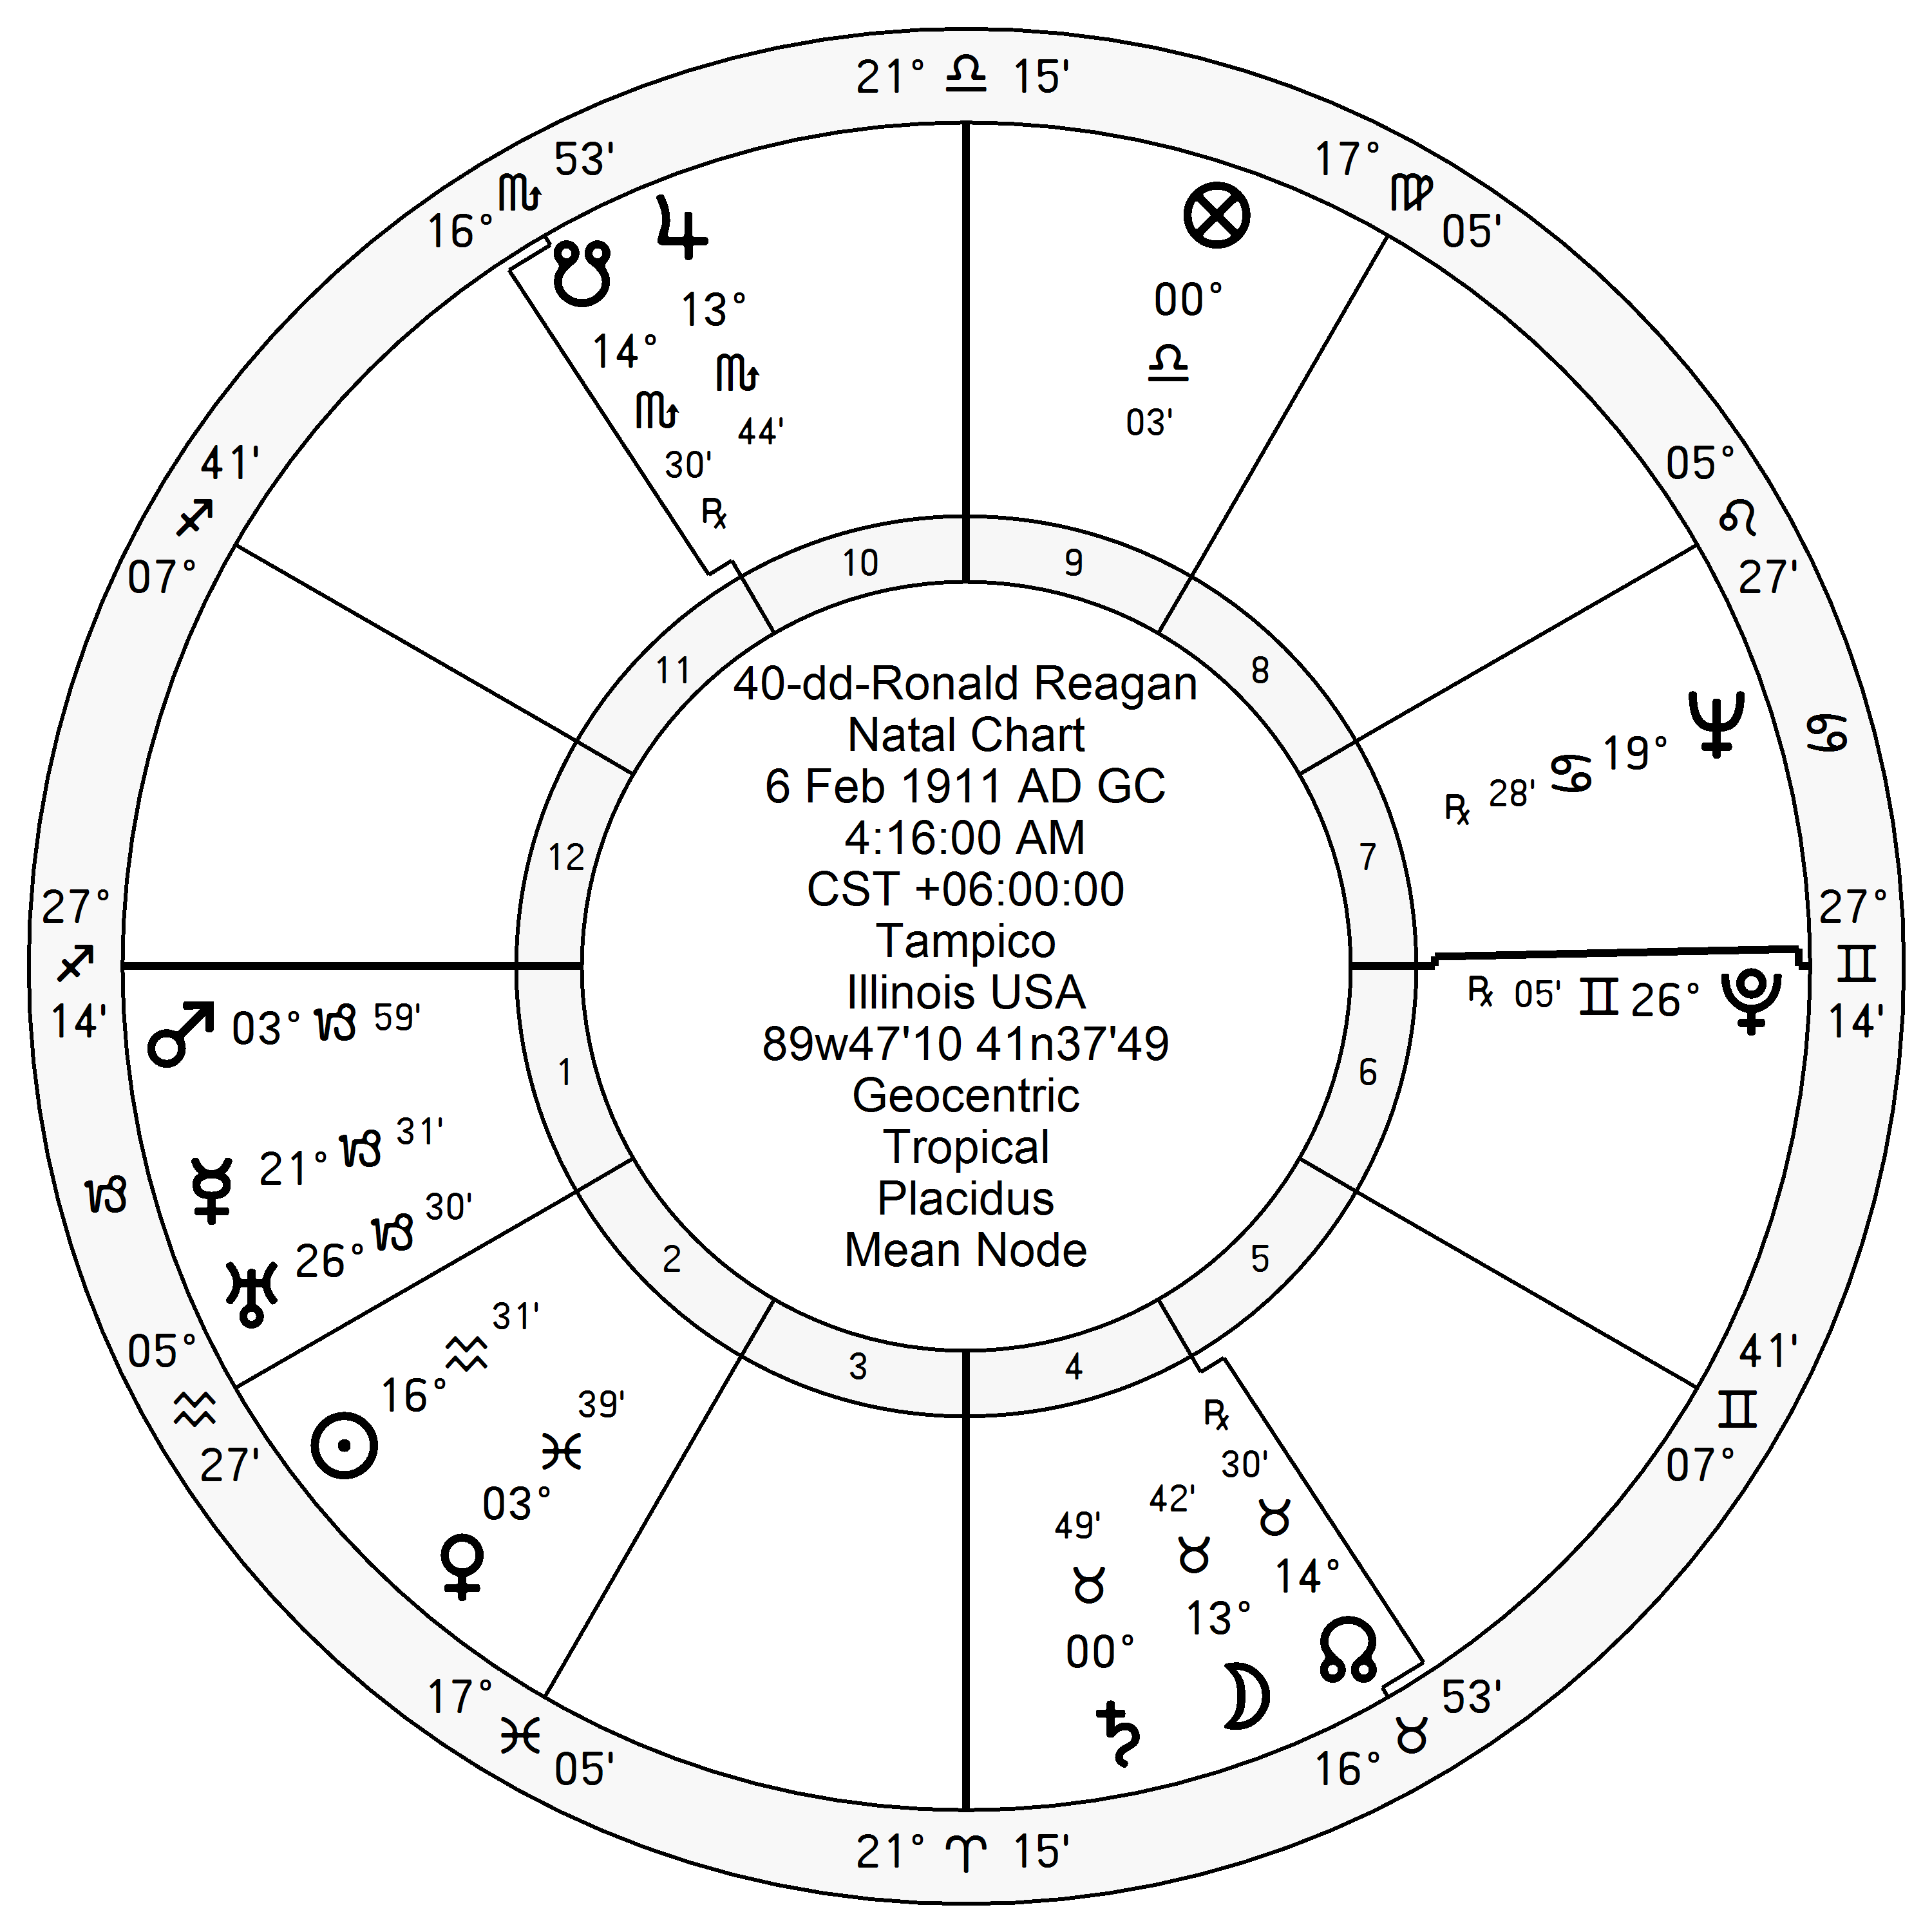
\includegraphics[width=0.9\textwidth]{charts/Reagan-dd.png}}
\fontsize{8pt}{9pt}\selectfont

\Saturn\, \Opposition\, P10, N10; \Square\, P1, N1 \\
\Venus\, \Trine\, P10, N10


\column{0.48\textwidth}
\vspace{-1em}
{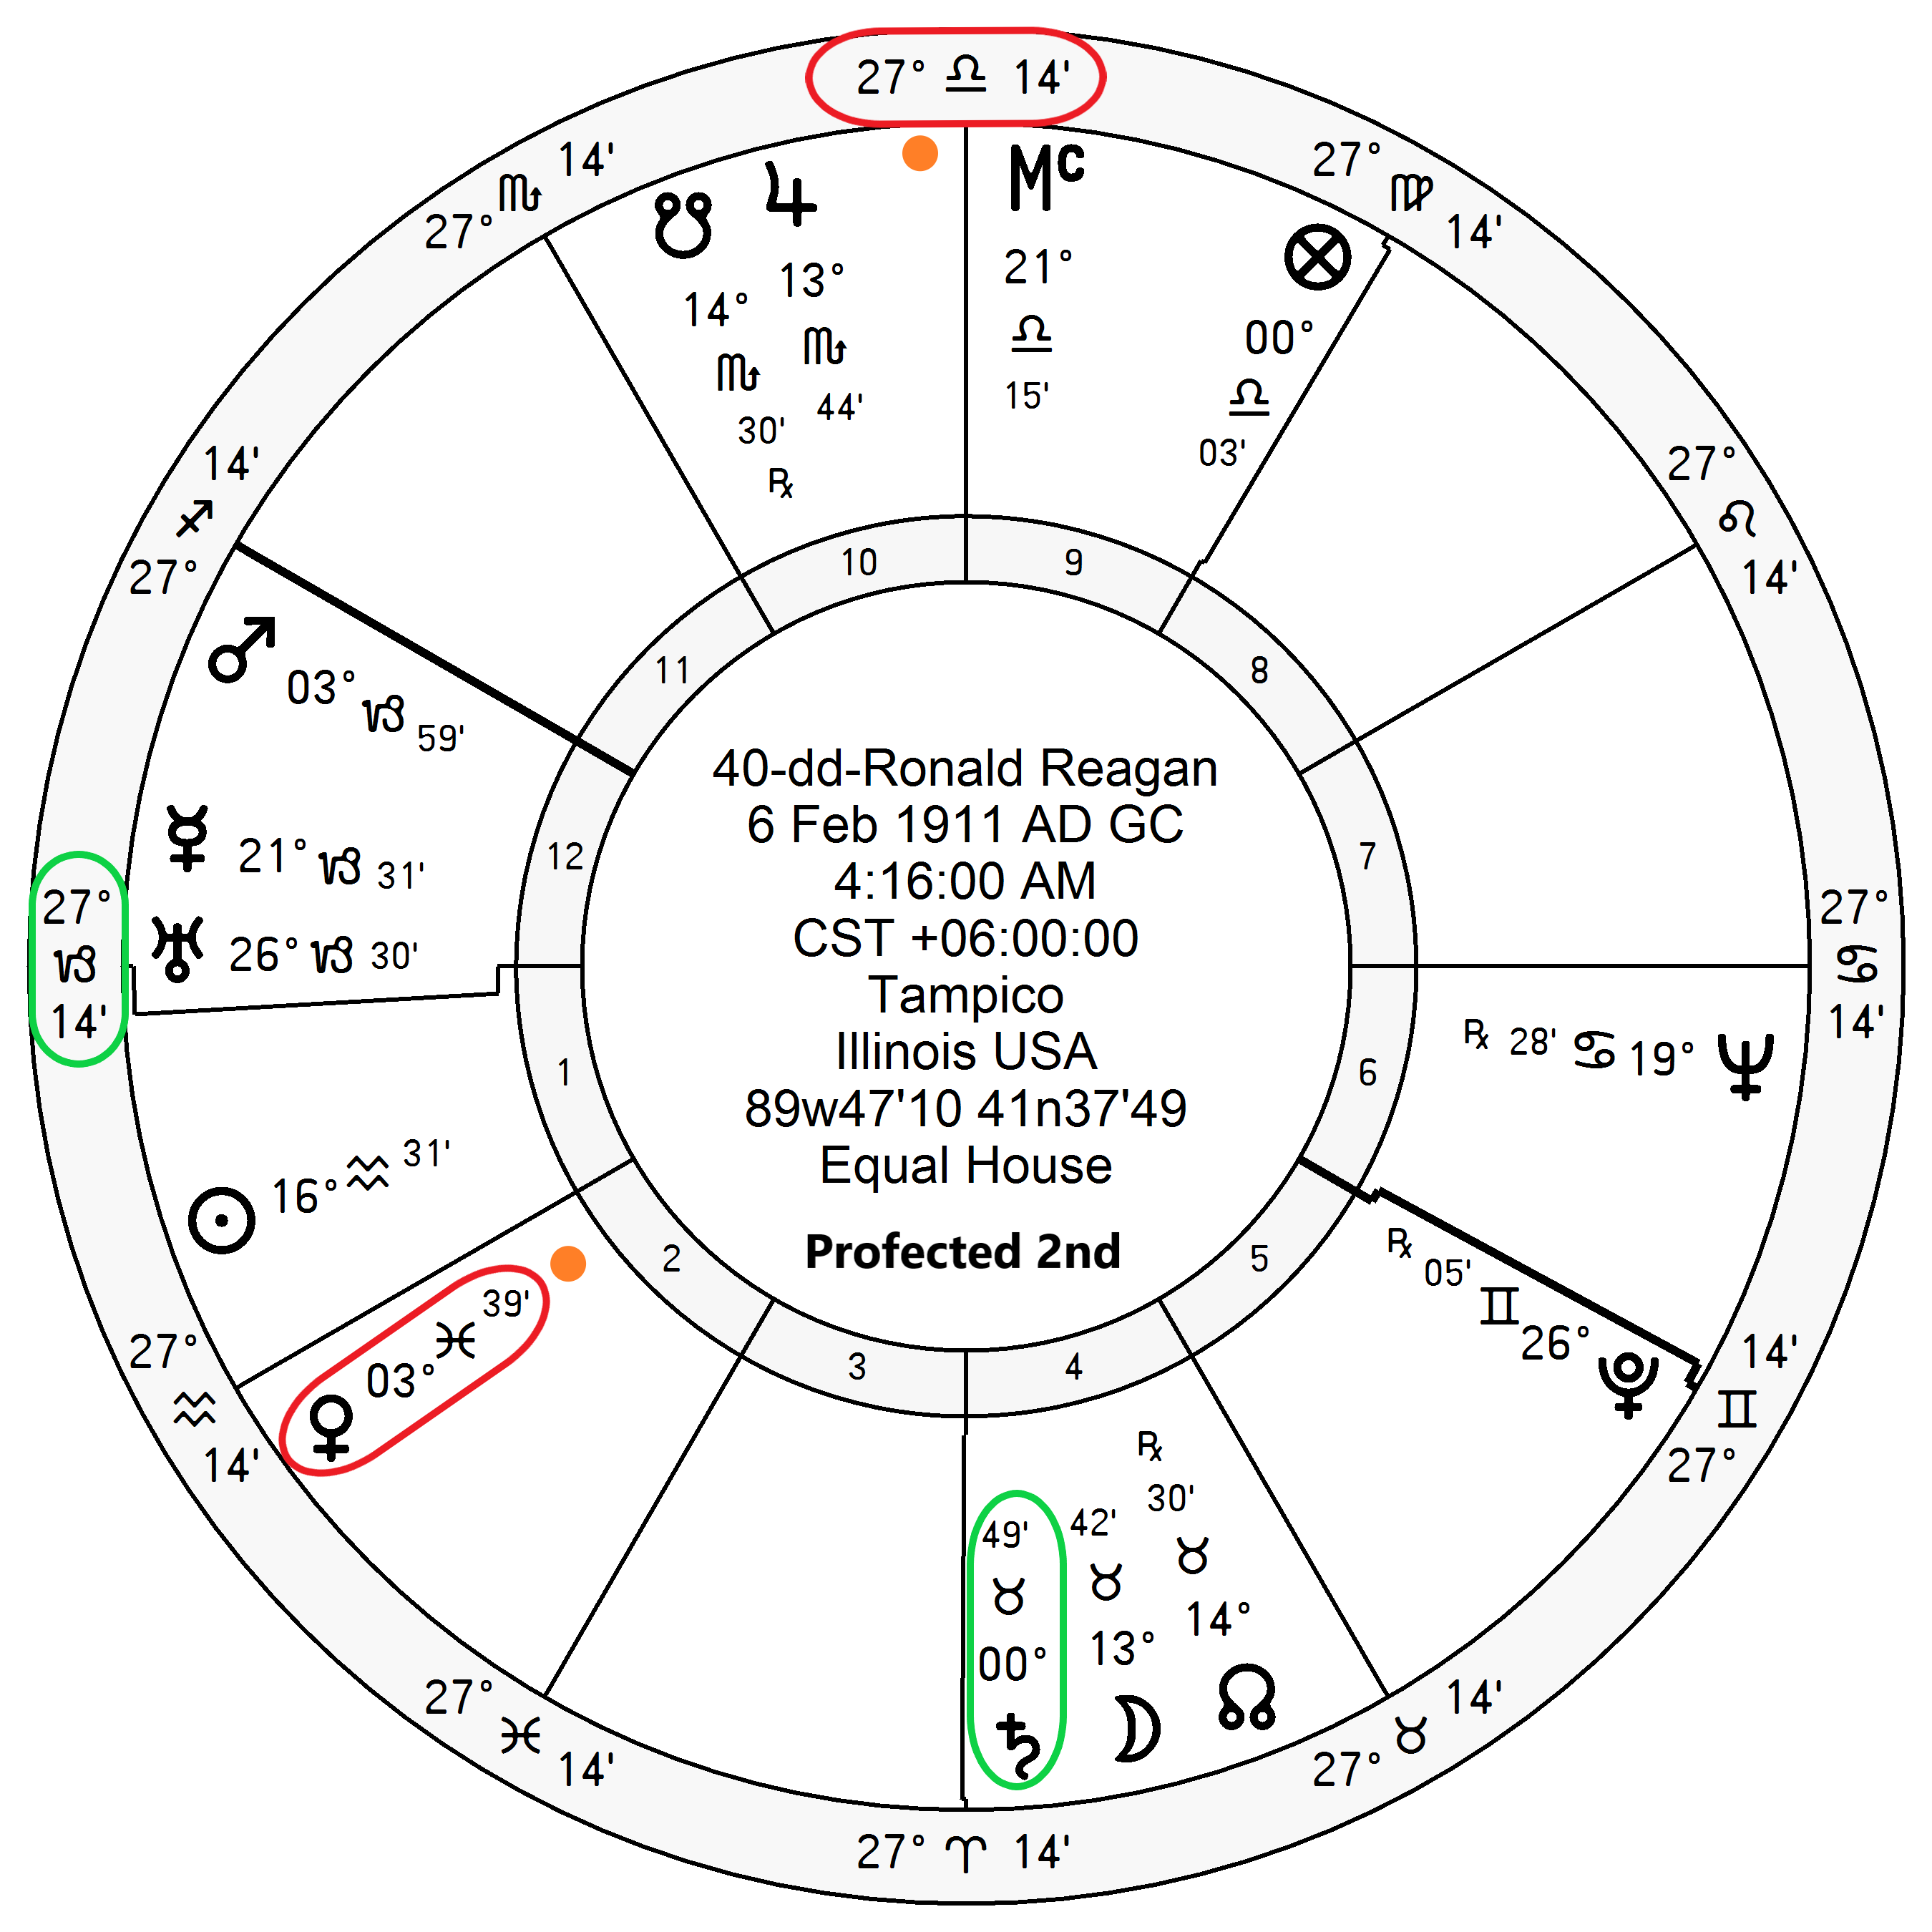
\includegraphics[width=0.9\textwidth]{charts/Reagan-dd-Prof-2nd.png}}
\fontsize{8pt}{9pt}\selectfont

\textbf{\dgreen P1=N1} 
	$\Rightarrow$ \Saturn\, $\Rightarrow$ P4/N4\\
\textbf{\red P10=N10}
	$\Rightarrow$ \Venus\, $\Rightarrow$ \textbf{\red P2/N2}\\
PE=\textbf{\red P10/N10}
	 $\Rightarrow$ \Venus\, $\Rightarrow$ \textbf{\red P2/N2}

\end{columns}
\end{frame}

% ===================================================
\begin{frame}[t]{Election November 6, 1984: Walter Mondale}
\small
\begin{columns}[T, onlytextwidth]
\column{0.48\textwidth}
\vspace{-1em}
{\includegraphics[width=0.9\textwidth]{charts/Mondale.png}}
\fontsize{8pt}{9pt}\selectfont

\Mars\, \Trine\, P10; in N10 \Square\, N1 \\
\Sun\, \Sextile\, P1 \\
\Mercury\, (burnt) \Sextile\, P1 

\column{0.48\textwidth}
\vspace{-1em}
{\includegraphics[width=0.9\textwidth]{charts/Mondale-Prof-9th.png}}
\fontsize{8pt}{9pt}\selectfont
\textbf{\dgreen P1}=N9
	$\Rightarrow$ \Mars\, $\Rightarrow$ P2/\textbf{\red N10}\\
\textbf{\red P10}=N6
	$\Rightarrow$ \Sun\, $\Rightarrow$ \textbf{\red P3/N11}\\
PE=\textbf{\red P11}/N7
	 $\Rightarrow$ \Mercury\, (burnt) $\Rightarrow$ \textbf{\red P3/N11}

\end{columns}
\end{frame}

%\subsection{Election November 8, 1988: *Bush vs Dukakis}
\begin{frame}[t]{Election November 8, 1988: *George H.W. Bush}
\small

\begin{columns}[T, onlytextwidth]
\column{0.48\textwidth}
\vspace{-1em}
{\includegraphics[width=0.9\textwidth]{charts/GHW-Bush.png}}
\fontsize{8pt}{9pt}\selectfont

\Jupiter\, \Sextile\, P10; \Opposition\, N10 \\
\Mercury\, \Trine\, P10 \\
\Mars\, partile \Trine\, \Saturn\, in P10; mitigated \Quincunx\, (\Opposition) N10 \\

\column{0.48\textwidth}
\vspace{-1em}
{\includegraphics[width=0.9\textwidth]{charts/GHW-Bush-Prof-5th.png}}
\fontsize{8pt}{9pt}\selectfont

\textbf{\dgreen P1=N5} 
	$\Rightarrow$ \Jupiter\, $\Rightarrow$ P12/N4\\
\textbf{\red P10=N2}
	$\Rightarrow$ \Mercury\, $\Rightarrow$ \textbf{\red P6/N10}\\
PE=\textbf{\dgreen P5}/N9
	 $\Rightarrow$ \Mars\, $\Rightarrow$ \textbf{\red P2/N6}

\end{columns}
\end{frame}

% ===================================================
\begin{frame}[t]{Election November 8, 1988: Michael Dukakis}
\small
\begin{columns}[T, onlytextwidth]
\column{0.48\textwidth}
\vspace{-1em}
{\includegraphics[width=0.9\textwidth]{charts/Dukakis.png}}
\fontsize{8pt}{9pt}\selectfont

\Saturn\, \Trine\, P10; \Trine\, N1 \\
\Venus\, \Sextile\, P10, \Sextile\, N10; \Opposition\, N1

\column{0.48\textwidth}
\vspace{-1em}
{\includegraphics[width=0.9\textwidth]{charts/Dukakis-Prof-8th.png}}
\fontsize{8pt}{9pt}\selectfont
\textbf{\dgreen P1=N9}
	$\Rightarrow$ \Saturn\, $\Rightarrow$ \textbf{\dgreen P2/N9}\\
\textbf{\red P10}=N6
	$\Rightarrow$ \Venus\, $\Rightarrow$ P12/N7\\
PE=\textbf{\dgreen P1/N9}
	 $\Rightarrow$ \Saturn\, $\Rightarrow$ \textbf{\dgreen P2/N9}

\end{columns}
\end{frame}

%\subsection{Election November 3, 1992: *Clinton vs Bush}
\begin{frame}[t]{Election November 3, 1992: *Bill Clinton}
\small

\begin{columns}[T, onlytextwidth]
\column{0.48\textwidth}
\vspace{-1em}
{\includegraphics[width=0.9\textwidth]{charts/Clinton.png}}
\fontsize{8pt}{9pt}\selectfont

\Sun\, in \Leo\, in P1 \Square\, P10; \Sextile\, N1 \\
\Venus\, \Sextile\, P1; in \Libra\, in N1 \Square\, N10

\column{0.48\textwidth}
\vspace{-1em}
{\includegraphics[width=0.9\textwidth]{charts/Clinton-Prof-11th.png}}
\fontsize{8pt}{9pt}\selectfont

\textbf{\dgreen P1=N11}
	$\Rightarrow$ \Sun\, $\Rightarrow$ \textbf{\dgreen P1/N11}\\
\textbf{\red P10}=N8
	$\Rightarrow$ \Venus\, $\Rightarrow$ \textbf{\red P3}/\textbf{\dgreen N1}\\
PE=\textbf{\red P3}\textbf{\dgreen /N1}
	 $\Rightarrow$ \Venus\, $\Rightarrow$ \textbf{\red P3}/\textbf{\dgreen N1}

\end{columns}
\end{frame}

% ===================================================
\begin{frame}[t]{Election November 3, 1992: George H.W. Bush}
\small
\begin{columns}[T, onlytextwidth]
\column{0.48\textwidth}
\vspace{-1em}
{\includegraphics[width=0.9\textwidth]{charts/GHW-Bush.png}}
\fontsize{8pt}{9pt}\selectfont

\Mars\, \Conjunction\, \SouthNode\, in P10; \Square\, N10 \\
\Saturn\, partile \Trine\, \Mars\, in P10; mitigated \Quincunx\, (\Opposition) N10 \\
\Sun\, \Trine\, P10; in N10, \Square\, N1 \\
\vspace{0.5em}
Another case of the \SouthNode\, weakening the candidate's chances?

\column{0.48\textwidth}
\vspace{-1em}
{\includegraphics[width=0.9\textwidth]{charts/GHW-Bush-Prof-9th.png}}
\fontsize{8pt}{9pt}\selectfont
\textbf{\dgreen P1}=N9
	$\Rightarrow$ \Mars\, (\Conjunction\, \SouthNode) 
	$\Rightarrow$ \textbf{\red P10/N6}\\
\textbf{\red P10=N6}
	$\Rightarrow$ \Saturn\, (partile \Trine\, \Mars) $\Rightarrow$ \textbf{\red P6}/N3\\
PE=P5/\textbf{\dgreen N1}
	 $\Rightarrow$ \Sun\, $\Rightarrow$P2/\textbf{\red N10}

\end{columns}
\end{frame}

%\subsection{Election November 5, 1996: *Clinton vs Dole}
\begin{frame}[t]{Election November 5, 1996: *Bill Clinton}
\small

\begin{columns}[T, onlytextwidth]
\column{0.48\textwidth}
\vspace{-1em}
{\includegraphics[width=0.9\textwidth]{charts/Clinton.png}}
\fontsize{8pt}{9pt}\selectfont

\Jupiter\, \Sextile\, P1; in N1 \Square\, N10 \\
\Mercury\, \Trine\, P1; in N10 \Sextile\, N1 \\
\Saturn\, in N10 \Sextile\, N1

\column{0.48\textwidth}
\vspace{-1em}
{\includegraphics[width=0.9\textwidth]{charts/Clinton-Prof-3rd.png}}
\fontsize{8pt}{9pt}\selectfont

\textbf{\dgreen P1=N3}
	$\Rightarrow$ \Jupiter\, $\Rightarrow$ P11/\textbf{\dgreen N1}\\
\textbf{\red P10}=N12
	$\Rightarrow$ \Mercury\, $\Rightarrow$ P9/\textbf{\red N10}\\
PE=\textbf{\dgreen P3}/N5
	 $\Rightarrow$ \Saturn\, $\Rightarrow$ P8/\textbf{\red N10}

\end{columns}
\end{frame}

% ===================================================
\begin{frame}[t]{Election November 5, 1996: Robert Dole}
\small
\begin{columns}[T, onlytextwidth]
\column{0.48\textwidth}
\vspace{-1em}
{\includegraphics[width=0.9\textwidth]{charts/Dole.png}}

\Mercury\, (burnt) \Trine\, P10; \Opposition\, N10 \\
\Jupiter\, \Trine\, P10; \Opposition\, N1 \\
\vspace{0.5em}
Dole has a burnt \Mercury\, and the \SouthNode\, in the 10th working against him.


\column{0.48\textwidth}
\vspace{-1em}
{\includegraphics[width=0.9\textwidth]{charts/Dole-Prof-2nd.png}}
\fontsize{8pt}{9pt}\selectfont
\textbf{\dgreen P1}=N3
	$\Rightarrow$ \Mercury\, (burnt) $\Rightarrow$ \textbf{\dgreen P2/N4}\\
\textbf{\red P10}=N12
	$\Rightarrow$ \Jupiter\, $\Rightarrow$ \textbf{\red P6}/N7\\
PE=P4/\textbf{\red N6}
	 $\Rightarrow$ \Mercury\, (burnt) $\Rightarrow$ \textbf{\dgreen P2/N4}

\end{columns}
\end{frame}

%\subsection{Election November 7, 2000: *Bush vs Gore}
\begin{frame}[t]{Election November 7, 2000: *George W Bush}
\small

\begin{columns}[T, onlytextwidth]
\column{0.48\textwidth}
\vspace{-1em}
{\includegraphics[width=0.9\textwidth]{charts/GW-Bush.png}}
\fontsize{7pt}{8pt}\selectfont

\Saturn\, \Trine\, P10; \Square\, N10 \\
\Mars\, \Sextile\, P10; \Trine\, N10 \\
\Mercury\, in N1 \Square\, N10, P10

\column{0.48\textwidth}
\vspace{-1em}
{\includegraphics[width=0.9\textwidth]{charts/GW-Bush-Prof-7th.png}}
\fontsize{8pt}{9pt}\selectfont

\textbf{\dgreen P1=N7}
	$\Rightarrow$ \Saturn\, $\Rightarrow$ P6/N12\\
\textbf{\red P10}=N4
	$\Rightarrow$ \Mars\, $\Rightarrow$ P8/N2\\
PE=P5/N11
	 $\Rightarrow$ \Mercury\, $\Rightarrow$ \textbf{\dgreen P7/N1}

\end{columns}
\end{frame}

% ===================================================
\begin{frame}[t]{Election November 7, 2000: Al Gore}
\small
\begin{columns}[T, onlytextwidth]
\column{0.48\textwidth}
\vspace{-1em}
{\includegraphics[width=0.9\textwidth]{charts/Gore.png}}
\fontsize{8pt}{9pt}\selectfont

\Jupiter\, in \Sagittarius\, in P1 \Square\, P10; \Trine\, N10, \Trine\, N1 \\
\Mercury\, \Opposition\, P10, \Square\, P1 \\
\Moon\, in \Capricorn\, in P1; \Square\, N10 \\
\vspace{0.5em}
There is not much between the two; Bush's radix connections to N10 are stronger.

\column{0.48\textwidth}
\vspace{-1em}
{\includegraphics[width=0.9\textwidth]{charts/Gore-Prof-5th.png}}
\fontsize{8pt}{9pt}\selectfont
\textbf{\dgreen P1=N5}
	$\Rightarrow$ \Jupiter\, $\Rightarrow$ \textbf{\dgreen P1/N5}\\
\textbf{\red P10}=N3
	$\Rightarrow$ \Mercury\, $\Rightarrow$ P4/\textbf{\red N8}\\
PE=\textbf{\red P8}/N12
	 $\Rightarrow$ \Moon\, $\Rightarrow$ \textbf{\dgreen P1/N5}

\end{columns}
\end{frame}

%\subsection{Election November 2, 2004: *Bush vs Kerry}
\begin{frame}[t]{Election November 2, 2004: *George W Bush}
\small

\begin{columns}[T, onlytextwidth]
\column{0.48\textwidth}
\vspace{-1em}
{\includegraphics[width=0.9\textwidth]{charts/GW-Bush.png}}
\fontsize{7pt}{8pt}\selectfont

\Mercury\, \Sextile\, P1; in N1 \Square\, N10 \\
\Jupiter\, \Trine\, P1; in mitigated \Quincunx\, (\Opposition) N10

\column{0.48\textwidth}
\vspace{-1em}
{\includegraphics[width=0.9\textwidth]{charts/GW-Bush-Prof-11th.png}}
\fontsize{8pt}{9pt}\selectfont

\textbf{\dgreen P1}=N11
	$\Rightarrow$ \Mercury\, $\Rightarrow$ \textbf{\dgreen P3/N1}\\
\textbf{\red P10}=N9
	$\Rightarrow$ \Jupiter\, $\Rightarrow$ P5/\textbf{\dgreen N3}\\
PE=P4/\textbf{\dgreen N3}
	 $\Rightarrow$ \Mercury\, $\Rightarrow$ \textbf{\dgreen P3/N1}

\end{columns}
\end{frame}

% ===================================================
\begin{frame}[t]{Election November 2, 2004: John Kerry}
\small
\begin{columns}[T, onlytextwidth]
\column{0.48\textwidth}
\vspace{-1em}
{\includegraphics[width=0.9\textwidth]{charts/Kerry.png}}
\fontsize{7pt}{8pt}\selectfont

Kerry's birth time is out of scope for the original study; the chart is based on Starkman's rectified time as given on Astrodatabank.\\
\vspace{0.5em}
\Jupiter\, \Trine\, P1, N1 \\
\Mercury\, \Trine\, P10, N10 \\
\Venus\, \Sextile\, P10

\column{0.48\textwidth}
\vspace{-1em}
{\includegraphics[width=0.9\textwidth]{charts/Kerry-Prof-1st.png}}
\fontsize{8pt}{9pt}\selectfont
\textbf{\dgreen P1}=N1
	$\Rightarrow$ \Jupiter\, $\Rightarrow$ P9/N9\\
\textbf{\red P10}=N10
	$\Rightarrow$ \Mercury\, $\Rightarrow$ P2/N2\\
PE=P11/N11
	 $\Rightarrow$ \Venus\, $\Rightarrow$ P12/N11

\end{columns}
\end{frame}

%\subsection{Election November 4, 2008: *Obama vs McCain}
\begin{frame}[t]{Election November 4, 2008: *Barack Obama}
\small

\begin{columns}[T, onlytextwidth]
\column{0.48\textwidth}
\vspace{-1em}
{\includegraphics[width=0.9\textwidth]{charts/Obama.png}}
\fontsize{7pt}{8pt}\selectfont

\Saturn\, in \Capricorn\, in P1 \Square\, P10; \Sextile\, N10 \\
\Venus\, \Trine\, P10; mit. \Quincunx\, (\Opposition) N10 \\
\Mars\, \Trine\, P1; \Square\, N10, \Opposition\, N1 

\column{0.48\textwidth}
\vspace{-1em}
{\includegraphics[width=0.9\textwidth]{charts/Obama-Prof-12th.png}}
\fontsize{8pt}{9pt}\selectfont

\textbf{\dgreen P1=N12}
	$\Rightarrow$ \Saturn\, $\Rightarrow$ \textbf{\dgreen P1/N12}\\
\textbf{\red P10}=N8
	$\Rightarrow$ \Venus\, $\Rightarrow$ P6/N5\\
PE=P4/N2
	 $\Rightarrow$ \Mars\, $\Rightarrow$ P9/N7

\end{columns}
\end{frame}

% ===================================================
\begin{frame}[t]{Election November 4, 2008: John McCain}
\small
\begin{columns}[T, onlytextwidth]
\column{0.48\textwidth}
\vspace{-1em}
{\includegraphics[width=0.9\textwidth]{charts/McCain.png}}
\fontsize{7pt}{8pt}\selectfont

\Jupiter\, in \Sagittarius\, in P1, N1; \Square\, P10, N10 \\
\Venus\, \Square\, P10, N10; \Opposition\, P1, N1 \\
\vspace{0.5em}
Looks stronger than Obama's charts; possibly \Saturn\, in P1 and N1 \Square\, \Jupiter\, and \Opposition\, \Venus\, denies what they promise in both times.

\column{0.48\textwidth}
\vspace{-1em}
{\includegraphics[width=0.9\textwidth]{charts/McCain-Prof-1st.png}}
\fontsize{8pt}{9pt}\selectfont
\textbf{\dgreen P1}=N1
	$\Rightarrow$ \Jupiter\, $\Rightarrow$ \textbf{\red P10/N10}\\
\textbf{\red P10=N10}
	$\Rightarrow$ \Jupiter\, $\Rightarrow$ \textbf{\red P10/N10}\\
PE=P3/N3
	 $\Rightarrow$ \Venus\, $\Rightarrow$ P7/N7

\end{columns}
\end{frame}

\subsection{Election November 6, 2012: *Obama vs Romney}
\begin{frame}[t]{Election November 6, 2012: *Barack Obama}
\small

\begin{columns}[T, onlytextwidth]
\column{0.48\textwidth}
\vspace{-1em}
{\includegraphics[width=0.9\textwidth]{charts/Obama.png}}
\fontsize{7pt}{8pt}\selectfont

\Venus\, \Trine\, N1; mit. \Quincunx\, (\Opposition) N10 \\
\Saturn\, \Trine\, P1, \Sextile\, N10 \\
\Moon\, in P1 \Square\, P10; \Opposition\, N10, \Square\, N1 \\
\vspace{0.5em}
\SouthNode\, in P10 appeared not to harm him; possibly because Romney had no aspects involving P10 or N10.

\column{0.48\textwidth}
\vspace{-1em}
{\includegraphics[width=0.9\textwidth]{charts/Obama-Prof-4th.png}}
\fontsize{8pt}{9pt}\selectfont

\textbf{\dgreen P1=N4}
	$\Rightarrow$ \Venus\, $\Rightarrow$ P2/N5\\
\textbf{\red P10}=\textbf{\dgreen N1}
	$\Rightarrow$ \Saturn\, $\Rightarrow$ P9/N12\\
PE=P3/N6
	 $\Rightarrow$ \Moon\, $\Rightarrow$ \textbf{\dgreen P1/N4}

\end{columns}
\end{frame}

% ===================================================
\begin{frame}[t]{Election November 6, 2012: Mitt Romney}
\small
\begin{columns}[T, onlytextwidth]
\column{0.48\textwidth}
\vspace{-1em}
{\includegraphics[width=0.9\textwidth]{charts/Romney.png}}
\fontsize{7pt}{8pt}\selectfont

\Mars\, \Trine\, P1; \Square\, N1 \\
\Sun\, \Trine\, P1; \Square\, N1 \\
\Mercury\, burnt \Trine\, P1; \Square\, N1


\column{0.48\textwidth}
\vspace{-1em}
{\includegraphics[width=0.9\textwidth]{charts/Romney-Prof-6th.png}}
\fontsize{8pt}{9pt}\selectfont
\textbf{\dgreen P1}=N6
	$\Rightarrow$ \Mars\, $\Rightarrow$ \textbf{\dgreen P5/N11}\\
\textbf{\red P10}=N4
	$\Rightarrow$ \Sun\, $\Rightarrow$ \textbf{\dgreen P5/N11}\\
PE=P8/N2
	 $\Rightarrow$ \Mercury\, $\Rightarrow$ \textbf{\dgreen P5/N11}

\end{columns}
\end{frame}

\subsection{Election November 8, 2016: *Trump vs Clinton}
\begin{frame}[t]{Election November 8, 2016: *Donald Trump}
\small

\begin{columns}[T, onlytextwidth]
\column{0.48\textwidth}
\vspace{-1em}
{\includegraphics[width=0.9\textwidth]{charts/Trump.png}}
\fontsize{7pt}{8pt}\selectfont

\Mercury\, in P1 \Square\, P10; \Sextile\, N1 \\
\Jupiter\, \Opposition\, P10, \Square\, P1; partile \Trine\, to \Uranus\, in N10 \\
\Venus\, in P1, \Square\, P10, \Sextile\, P1, N10

\column{0.48\textwidth}
\vspace{-1em}
{\includegraphics[width=0.9\textwidth]{charts/Trump-Prof-11th.png}}
\fontsize{8pt}{9pt}\selectfont

\textbf{\dgreen P1}=N11
	$\Rightarrow$ \Mercury\, $\Rightarrow$ \textbf{\dgreen P1/N11}\\
\textbf{\red P10}=N8
	$\Rightarrow$ \Jupiter\,\Retrograde $\Rightarrow$ P4/N2\\
PE=P5/N3
	 $\Rightarrow$ \Venus\, $\Rightarrow$ \textbf{\dgreen P1/N11}

\end{columns}
\end{frame}

% ===================================================
\begin{frame}[t]{Election November 8, 2016: Hilary Clinton}
\small
\begin{columns}[T, onlytextwidth]
\column{0.48\textwidth}
\vspace{-1em}
{\includegraphics[width=0.9\textwidth]{charts/Hillary.png}}
\fontsize{7pt}{8pt}\selectfont

\Jupiter\, \Trine\, P1; \Square\, N10 

\column{0.48\textwidth}
\vspace{-1em}
{\includegraphics[width=0.9\textwidth]{charts/Hillary-Prof-10th.png}}
\fontsize{8pt}{9pt}\selectfont
\textbf{\dgreen P1=N11}
	$\Rightarrow$ \Jupiter\, $\Rightarrow$ \textbf{\dgreen P9/N6}\\
\textbf{\red P10}=N7
	$\Rightarrow$ \Jupiter\, $\Rightarrow$ \textbf{\dgreen P9/N6}\\
PE=\textbf{\dgreen P1/N11}
	 $\Rightarrow$ \Jupiter\, $\Rightarrow$ \textbf{\dgreen P9/N6}

\end{columns}
\end{frame}

\subsection{Election November 3, 2020: *Biden vs Trump}
\begin{frame}[t]{Election November 3, 2020: *Joe Biden}
\small

\begin{columns}[T, onlytextwidth]
\column{0.48\textwidth}
\vspace{-1em}
{\includegraphics[width=0.9\textwidth]{charts/Biden.png}}
\fontsize{7pt}{8pt}\selectfont

\Venus\, burnt \Square\, P10, \Opposition\, P1; \Sextile\, N10 \\
\Saturn\, \Trine\, P10; \Opposition\, N1, \Square\, N10 \\
\Mars\, \Square\, P10, \Opposition\, P1; \Sextile\, N10

\column{0.48\textwidth}
\vspace{-1em}
{\includegraphics[width=0.9\textwidth]{charts/Biden-Prof-6th.png}}
\fontsize{8pt}{9pt}\selectfont

\textbf{\dgreen P1}=N6
	$\Rightarrow$ \Venus\, $\Rightarrow$ \textbf{\dgreen P7/N12}\\
\textbf{\red P10}=N3
	$\Rightarrow$ \Saturn\,\Retrograde\, $\Rightarrow$ P2/\textbf{\dgreen N7}\\
PE=\textbf{\dgreen P12}/N5
	 $\Rightarrow$ \Mars\, $\Rightarrow$ \textbf{\dgreen P7}/N11

\end{columns}
\end{frame}

% ===================================================
\begin{frame}[t]{Election November 3, 2020: Donald Trump}
\small
\begin{columns}[T, onlytextwidth]
\column{0.48\textwidth}
\vspace{-1em}
{\includegraphics[width=0.9\textwidth]{charts/Trump.png}}
\fontsize{8pt}{9pt}\selectfont

\Venus\, \Trine\, P1, \Sextile\, P10 \\
\Moon\, \Conjunction\, \SouthNode\,, \Trine\, P10; \Opposition\, N10, \Square\, N1 \\
\Saturn\, \Trine\, P1; \Sextile\, N1 \\
\vspace{0.5em}
Only one hard aspect involving the 10th and it's weakened by the conjunction with the \SouthNode\,

\column{0.48\textwidth}
\vspace{-1em}
{\includegraphics[width=0.9\textwidth]{charts/Trump-Prof-3rd.png}}
\fontsize{8pt}{9pt}\selectfont
\textbf{\dgreen P1}=N3
	$\Rightarrow$ \Venus\, $\Rightarrow$ \textbf{\red P9/N11}\\
\textbf{\red P10=N11}
	$\Rightarrow$ \Moon\, \Conjunction\, \SouthNode\, $\Rightarrow$ P2/N4\\
PE=\textbf{\dgreen P5/N6}
	 $\Rightarrow$ \Saturn\, $\Rightarrow$ \textbf{\red P9/N11}

\end{columns}
\end{frame}

\section{Initial Conclusions}
\begin{frame}[t]{Initial Conclusions}
\centering
\begin{minipage}{0.9\textwidth}
\begin{itemize}
\item Hard aspects from the planets managing the times, especially those involving P10 and N10, appear to win out over soft aspects with the possible exception of a partile trine involving a planet in or ruling the 10th in either time
\vspace{0.5em}

\item A burnt \Mercury\, as one of the planets managing the times appears to ensure a loss
\vspace{0.5em}

\item The \SouthNode\, in N10 appears to weaken chances (see Wilkie, McGovern); in P10 it gives mixed indications: Reagan, Obama, and Biden all had it in P10 and won while George H.W. Bush had it in P10 with the ruler of P1 and lot and Dole had it in P10 with Uranus and lost but he also had a burnt \Mercury\, ruling P1 \Trine\, P10
\end{itemize}
\end{minipage}
\end{frame}
\subsection{Election November 5, 2024: Biden vs Trump}
\begin{frame}[t]{Election November 5, 2024: Joe Biden}
\small

\begin{columns}[T, onlytextwidth]
\column{0.48\textwidth}
\vspace{-1em}
{\includegraphics[width=0.9\textwidth]{charts/Biden.png}}
\fontsize{7pt}{8pt}\selectfont

\Mercury\, burnt \Sextile\, P1, \Sextile\, N10 \\
\Sun\, \Sextile\, P10; \Sextile\, N10

\column{0.48\textwidth}
\vspace{-1em}
{\includegraphics[width=0.9\textwidth]{charts/Biden-Prof-10th.png}}
\fontsize{8pt}{9pt}\selectfont

\textbf{\dgreen P1}=N10
	$\Rightarrow$ \Mercury\, (burnt) $\Rightarrow$ \textbf{\dgreen P3/N12}\\
\textbf{\red P10}=N7
	$\Rightarrow$ \Mercury\, (burnt) $\Rightarrow$ \textbf{\dgreen P3/N12}\\
PE=\textbf{\dgreen P12}/N9
	 $\Rightarrow$ \Sun\, $\Rightarrow$ \textbf{\dgreen P3/N12}

\end{columns}
\end{frame}

% ===================================================
\begin{frame}[t]{Election November 5, 2024: Donald Trump}
\small
\begin{columns}[T, onlytextwidth]
\column{0.48\textwidth}
\vspace{-1em}
{\includegraphics[width=0.9\textwidth]{charts/Trump.png}}
\fontsize{6pt}{7pt}\selectfont

\Saturn\, mit. \Quincunx\, (\Opposition) P10, \Trine\, P1, partile \Sextile\, to N2 \\
\Mars\, \Trine\, P10; \Square\, N10 \\
\Mercury\, \Trine\, P1, mit. \Quincunx\, (\Opposition) P10; \Sextile\, N1 \\
\vspace{0.5em}
Trump looks like the winner (assuming both are candidates on election day). The \SouthNode\, \Conjunction\, \Moon\, in P10 could cause problems, possibly GOP won't do well overall, weakening his control over Congress or the Senate, or both (\Moon\, rules P6, N11).

\column{0.48\textwidth}
\vspace{-1em}
{\includegraphics[width=0.9\textwidth]{charts/Trump-Prof-7th.png}}
\fontsize{8pt}{9pt}\selectfont
\textbf{\dgreen P1}=N7
	$\Rightarrow$ \Saturn\, $\Rightarrow$ \textbf{\dgreen P5/N11}\\
\textbf{\red P10}=N4
	$\Rightarrow$ \Mars\, $\Rightarrow$ P6/N12\\
PE=\textbf{\dgreen P5/N11}
	 $\Rightarrow$ \Mercury\, $\Rightarrow$ \textbf{\dgreen P5/N11}

\end{columns}
\end{frame}
% ===================================================
\begin{frame}[t]{Election November 5, 2024: Kamala Harris}
\small
\begin{columns}[T, onlytextwidth]
\column{0.48\textwidth}
\vspace{-1em}
{\includegraphics[width=0.9\textwidth]{charts/Harris.png}}
\fontsize{6pt}{7pt}\selectfont

\Mercury\, in P5 (elections) with \Sun\, (out of sign \Conjunction) with both in out of sign \Opposition\, to \Moon\, (changed conditions bring opposition?) \Trine\, MC \\
\Jupiter\, \Conjunction\, 12th (enemies) \Sextile\, 10th \\
\vspace{0.5em}
Possible the administration will put her in place as the candidate; the \NorthNode\, on the Asc could indicate a change in her status (MC is at the nodal bending) but it may not go well for her person (Fortune with \SouthNode). Chart does not look strong enough to pull off a win.

\column{0.48\textwidth}
\vspace{-1em}
{\includegraphics[width=0.9\textwidth]{charts/Harris-Prof-1st.png}}
\fontsize{8pt}{9pt}\selectfont
\textbf{\dgreen P1=N1}
	$\Rightarrow$ \Mercury\, $\Rightarrow$ \textbf{\dgreen P5/N5}\\
\textbf{\red P10}=N10
	$\Rightarrow$ \Jupiter\, $\Rightarrow$ P11/N12\\
PE=\textbf{\dgreen P1/N1}
	 $\Rightarrow$ \Mercury\, $\Rightarrow$ \textbf{\dgreen P5/N5}

\end{columns}
\end{frame}
% ===================================================
\begin{frame}[t]{Election November 5, 2024: J.D. Vance}
\small
\begin{columns}[T, onlytextwidth]
\column{0.48\textwidth}
\vspace{-1em}
{\includegraphics[width=0.9\textwidth]{charts/Vance.png}}
\fontsize{6pt}{7pt}\selectfont

\Jupiter\ is retrograde separating from \Trine\ (3°) of \Mercury\ (L2,L11) and \Sextile\ of \Saturn\ (L6,L7) and applying to and out of sign \Conjunction\ (5°) with \Neptune\, and out of sign \Sextile\ (4°) of \Pluto.\\
\vspace{0.5em} \tiny
There are no hard aspects, the \Neptune, \Pluto\ contacts could indicate some nefarious and coercive tactics in connection with the election. The \Mercury, \Saturn\, contacts point to considerable (\Mercury\ L2 in domicile in 1st), long-standing (\Saturn\ stationary direct) financial support from powerful, behind the scenes men (\Trine\Sun\ in 12th). The out of sign might signify him taking power under changed conditions after the election.


\column{0.48\textwidth}
\vspace{-1em}
{\includegraphics[width=0.9\textwidth]{charts/Vance-Prof-5th.png}}
\fontsize{8pt}{9pt}\selectfont
\textbf{\dgreen P1=N5}
	$\Rightarrow$ \Jupiter\small\Retrograde, $\Rightarrow$ \textbf{\dgreen P1/N5}\\
\textbf{\red P10}=N2
	$\Rightarrow$ \Mercury\, $\Rightarrow$ P9/\dgreen{N1}\\
PE=\textbf{\dgreen P4/N8}
	 $\Rightarrow$ \Jupiter\small\Retrograde, $\Rightarrow$ \textbf{\dgreen P1/N5}

\end{columns}
\end{frame}




\end{document}